%MIT License
%
%Copyright (c) 2018 Chen Wang [https://chenwang.site]
%
%Permission is hereby granted, free of charge, to any person obtaining a copy
%of this software and associated documentation files (the "Software"), to deal
%in the Software without restriction, including without limitation the rights
%to use, copy, modify, merge, publish, distribute, sublicense, and/or sell
%copies of the Software, and to permit persons to whom the Software is
%furnished to do so, subject to the following conditions:
%
%The above copyright notice and this permission notice shall be included in all
%copies or substantial portions of the Software.
%
%THE SOFTWARE IS PROVIDED "AS IS", WITHOUT WARRANTY OF ANY KIND, EXPRESS OR
%IMPLIED, INCLUDING BUT NOT LIMITED TO THE WARRANTIES OF MERCHANTABILITY,
%FITNESS FOR A PARTICULAR PURPOSE AND NONINFRINGEMENT. IN NO EVENT SHALL THE
%AUTHORS OR COPYRIGHT HOLDERS BE LIABLE FOR ANY CLAIM, DAMAGES OR OTHER
%LIABILITY, WHETHER IN AN ACTION OF CONTRACT, TORT OR OTHERWISE, ARISING FROM,
%OUT OF OR IN CONNECTION WITH THE SOFTWARE OR THE USE OR OTHER DEALINGS IN THE
%SOFTWARE.
\documentclass[12pt,a4paper]{Thesis} % Paper size, default font size and one-sided paper

\graphicspath{%
	{./Pictures/}%
	{./Figures/}%
}
\DeclareMathOperator{\Tr}{Tr}
\let\savedegree\degree
\let\degree\relax
\let\savedegree\ref
\let\rem\relax
\usepackage{adjustbox}
\usepackage{amsmath}
\usepackage{siunitx}
\usepackage{amssymb}
\usepackage{multirow}
\usepackage{wrapfig}
\usepackage{enumitem}
\usepackage{subcaption}
\usepackage{mathtools}
\usepackage{lipsum}
\usepackage[ruled,vlined,noresetcount]{algorithm2e}
%\usepackage{algpseudocode}
\usepackage[square, numbers, comma, sort&compress]{natbib} % Use the natbib reference package - read up on this to edit the reference style; if you want text (e.g. Smith et al., 2012) for the in-text references (instead of numbers), remove 'numbers'

\title{\ttitle} % Defines the thesis title - don't touch this

%extra packages
\usepackage{float}
\usepackage{color,soul}
\usepackage{enumerate}
\usepackage{Styles/mydefs}
\usepackage{tabularx}
\usepackage{booktabs}
\usepackage{tikz}
\usepackage{tikzscale}
\usepackage{comment}
\usetikzlibrary{positioning, positioning,fit,decorations.pathreplacing,arrows.meta}
\DeclareMathOperator*{\argmin}{argmin}
\DeclareMathOperator*{\argmax}{argmax}

\begin{document}

\frontmatter % Use roman page numbering style (i, ii, iii, iv...) for the pre-content pages

\setstretch{1.3} % Line spacing of 1.3
% Define the page headers using the Fr package and set up for one-sided printing

\pagestyle{fancy} % Finally, use the "fancy" page style to implement the FancyHdr headers
\fancyhead{}   %clear all fields
\fancyhead[LO]{\sl{\leftmark}}
\fancyhead[RE]{\sl{\rightmark}}
\fancyhead[LE,RO]{\thepage}


%----------------------------------------------------------------------------------------
%	TITLE PAGE
%----------------------------------------------------------------------------------------

%%% Use \maketitleforreview instead of \maketitle, if you want a PLAIN TITLE PAGE

\maketitle
% \maketitleforreview


% ----------------------------------------------------------------------------------------
% 	DECLARATION PAGE
% ----------------------------------------------------------------------------------------

\thesisdeclareOriginality{I hereby certify that the work embodied in this thesis is the result of original research, is free of plagiarised materials, and has not been submitted for a higher degree to any other University or Institution.}{Aug. 2018}{Styles/signature.png}

\thesisdeclareSupervisor{I have reviewed the content and presentation style of this thesis and declare it is free of plagiarism and of sufficient grammatical clarity to be examined.  To the best of my knowledge, the research and writing are those of the candidate except as acknowledged in the Author Attribution Statement. I confirm that the investigations were conducted in accord with the ethics policies and integrity standards of Nanyang Technological University and that the research data are presented honestly and without prejudice.}{Mar. 2019}{Styles/signature.png}

\thesisdeclareAuthorship{Please select one of the following; *delete as appropriate:
\\
*(A) This thesis does not contain any materials from papers published in peer-reviewed journals or from papers accepted at conferences in which I am listed as an author.
\\
*(B) This thesis contains material from [x number] paper(s) published in the following peer-reviewed journal(s) / from papers accepted at conferences in which I am listed as an author.}
{Please amend the typical statements below to suit your circumstances if (B) is selected.

	Chapter 4 is published as {\color{blue}D.T. Murphy, S. Schmid, J.R. Hester, P.E.R. Blanchard, and W. Miiller.  Coordination site disorder in spinel-type LiMnTiO4.  Inorganic Chemistry 54, 4636-4643 (2015). DOI: 10.1021/ic502747p.}

	The contributions of the co-authors are as follows:
	\begin{itemize}[topsep=1pt,itemsep=1pt,partopsep=1pt, parsep=1pt]
		\item A/Prof Schmid provided the initial project direction and edited the manuscript drafts.
		\item I prepared the manuscript drafts.  The manuscript was revised by Dr Hester and Dr. Blanchard.
		\item I co-designed the study with A/Prof Siegbert Schmid and performed all the laboratory work at the School of Materials Science and Engineering and the Singapore Synchrotron Light Source.   I also analyzed the data.
		\item All microscopy, including sample preparation, was conducted by me in the Facility for Analysis, Characterization, Testing and Simulation.
		\item Dr James Hester assisted in the collection of the neutron powder diffraction data.
		\item Dr Peter Blanchard assisted in the interpretation of the X-ray absorption spectroscopy data and carried out the spectral interpretation.
		\item Dr Wojciech Miiller assisted in the collection and provide guidance in the interpretation of the magnetic measurement data.
	\end{itemize}

	Chapter 5 is published as {\color{blue}H. V Doan, B. Yao, Y. Fang, A. Sartbaeva, U. Hintermair, V. P Ting, Controlled Formation of Hierarchical Metal-Organic Frameworks using CO2 Expanded Solvent Systems. In press, ACS Sustainable Chemistry \& Engineering (2017). DOI: 10.1021/acssuschemeng.7b01429}

	The contributions of the co-authors are as follows:
	\begin{itemize}[topsep=1pt,itemsep=1pt,partopsep=1pt, parsep=1pt]
		\item Prof Ting suggested the materials area and edited the manuscript drafts.
		\item I wrote the drafts of the manuscript.  The manuscript was revised together with Dr. Sartbaeva and Dr. Yao.
		\item II performed all the materials synthesis, collected X-ray diffraction patterns and visible light spectra, carried transmission electron microscopy, and conducted data evaluation.
		\item IDr. Y. Fang conducted the Rietveld analysis of the powder X-ray diffraction data and single crystal structure determinations.
		\item IDr U. Hintermair conducted the molecular dynamics simulations.
		\item IMs. A. Sartbaeva prepared the samples for electron microscopy.
	\end{itemize}
}{Mar. 2019}{Styles/signature.png}

% ----------------------------------------------------------------------------------------
% 	ACKNOWLEDGEMENTS
% ----------------------------------------------------------------------------------------

\setstretch{1.3} % Reset the line-spacing to 1.3 for body text (if it has changed)

\acknowledgements{\addtocontents{toc}{\vspace{0.8em}} % Add a gap in the Contents, for aesthetics

I wish to express my greatest gratitude to my advisor, Assoc. Prof Xueyan Tang. Without his full support, it would be impossible for me to 

% \begin{flushright}
% \emph{Jinming Xu, December 2015}
% \end{flushright}
}

%----------------------------------------------------------------------------------------
%	QUOTATION PAGE
%----------------------------------------------------------------------------------------

\pagestyle{empty} % No headers or footers for the following pages
\emph{``If I had one hour to save the world, I would spend 55 minutes defining the problem and only five minutes finding the solution."}

\begin{flushright}
---Einstein, Albert
\end{flushright}
\null\vfill % Add some space to move the quote down the page a bit

\begin{center}
\large{To my dear family}
\end{center}
\vfill\vfill\null % Add some space at the bottom to position the quote just right
\cleardoublepage % Start a new page and make the next page a right-hand (odd-numbered) page, producing a blank page if necessary

\pagestyle{fancy} % Return the page headers back to the "fancy" style
\fancyhead{}   %clear all fields
\fancyhead[LO]{\sl{\leftmark}}
\fancyhead[RE]{\sl{\rightmark}}
\fancyhead[LE,RO]{\thepage}

%----------------------------------------------------------------------------------------
%	ABSTRACT PAGE
%----------------------------------------------------------------------------------------

\addtotoc{Abstract} % Add the "Abstract" page entry to the Contents

\abstract{\addtocontents{toc}{\vspace{0.8em}}}% Add a gap in the Contents, for aesthetics

% 1. The Problem 2. The Issues 3. The Approach 4. The Results 5. The Experiments 6. The Applications

The proliferation of computing-intensive workloads has firmly established geo-distributed architectures—spanning cloud platforms, interconnected data centers, and high-performance computing clusters—as the standard paradigm for modern large-scale data processing. To exploit data locality and minimize bandwidth consumption, these systems routinely distribute computing jobs into multiple localized tasks deployed across disparate geographical sites where the requisite input data reside. This framework has become highly prevalent across diverse application domains, including sensor networks, climate modeling, and large-scale machine learning. However, the heterogeneous nature of these environments introduces profound challenges in resource allocation and job scheduling. Due to the imbalanced distribution of workloads and varying site capacities, classical single-cluster scheduling mechanisms often precipitate resource bottlenecks, system inefficiencies, and severe job starvation. Furthermore, while geo-distributed sites are typically interconnected via well-provisioned networks, the strategic utilization of these network resources to transfer data and computational demands across sites remains a complex, NP-hard problem. More critically, a fundamental dichotomy exists between optimizing system efficiency (e.g., minimizing average job response time) and guaranteeing equitable resource allocation among competing jobs. Purely efficiency-driven algorithms often compromise fairness, while strict fairness-oriented policies inevitably degrade overall throughput. To address these multi-dimensional challenges, this dissertation systematically investigates resource allocation and job scheduling in geo-distributed systems, proposing a series of novel, network-aware scheduling frameworks that leverage inter-site bandwidth to synergistically optimize processing efficiency and rigorous fairness guarantees. 

The first phase of this research focuses on redefining equitable resource allocation in distributed execution environments by integrating network transmission capabilities. Existing studies on fair resource allocation, such as Max-min Fairness and Dominant Resource Fairness, predominantly operate under single-site assumptions where all systemic resources are homogeneously accessible. In geo-distributed systems, however, evaluating fairness solely at the localized level is inherently flawed; a resource-intensive job constrained to a low-capacity site may suffer from highly unfair allocations despite monopolizing local resources. To resolve this, this dissertation proposes Dynamic Aggregate Max-min Fairness (DAMF), a pioneering resource allocation policy that leverages spare inter-site network bandwidth to dynamically transfer data and computation demands. DAMF mandates that the aggregate resource allocation for each job across all computational sites achieves max-min fairness over the entirety of the system's demand transmission and allocation solution space. Theoretically, this research rigorously proves that the DAMF policy satisfies three critical axiomatic properties of fair division: Pareto efficiency, envy-freeness, and strategy-proofness. From a practical standpoint, the study develops comprehensive algorithms and a fast approximation tailored to compute optimal demand transmissions and precise DAMF resource allocations subject to dynamic demand distributions and strict network capacity constraints. Extensive experimental evaluations demonstrate that DAMF significantly outperforms conventional baseline policies, successfully achieving superior fairness metrics among competing jobs while simultaneously enhancing the aggregate utility of the distributed system. 

Building upon the integration of network resources, the second phase of this dissertation pivots to the optimization of system efficiency, specifically targeting the minimization of average job response time in distributed environments. In geo-distributed architectures, a job's completion time is strictly dictated by the completion of its terminal task across all executing sites. Consequently, traditional efficiency-centric strategies like Shortest Remaining Processing Time (SRPT), which are optimal for single-site clusters, yield deeply suboptimal results in distributed settings. The problem is exacerbated by the intricate interdependencies between the local execution order of jobs and the cross-site transmission of tasks: transferring a single task can fundamentally alter the global optimal execution sequence, while a newly proposed execution order may necessitate a divergent transmission strategy. To disentangle this complexity, this research introduces Workload-Aware Selection with Transmission (WAST), an integrated job scheduling algorithm designed to concurrently compute the global execution order and optimal inter-site task transmissions. WAST systematically formulates the response-time minimization objective into a sequence of optimization problems, which are elegantly transformed into multiple minimum-cost flow problems solvable by advanced operational research solvers (e.g., OR-Tools, Cplex, GUROBI). To mitigate the substantial computational overhead inherent to the massive solution space, a highly efficient heuristic approximation algorithm is further proposed without significantly compromising scheduling fidelity. Driven by real-world production cluster traces from Alibaba, the empirical validation confirms that both WAST and its heuristic counterpart compute near-optimal execution sequences and transmission strategies, drastically reducing average job response times, particularly under highly skewed spatial workload distributions.

The final phase of the dissertation unifies the dual objectives by establishing a robust framework that successfully reconciles the inherent trade-off between scheduling efficiency and long-term fairness. Recognizing that instantaneous fairness can cripple system throughput and pure efficiency can induce prolonged job starvation, this research introduces a stringent long-term fairness criterion inspired by the concept of "protective scheduling." Under this criterion, a scheduling policy must guarantee that no job experiences a completion time later than it would under a baseline distributed Processor Sharing (PS) protocol, which theoretically guarantees equitable capacity sharing among all active jobs. To operationalize this, the dissertation formulates the distributed protective scheduling problem by constructing a mathematically rigorous slack system characterized by dual perspectives: a global view and an independent view. Crucially, mathematical proofs presented in this study reveal that, owing to the volatile nature of dynamic job arrivals and shifting load distributions, no purely globally order-based scheduling policy can maintain strict protectiveness. To transcend this theoretical limitation, a novel heuristic algorithmic framework, denoted as PFSP\_x, is developed. PFSP\_x acts as a hybrid scheduling engine that strictly enforces the protective fairness boundaries while aggressively optimizing the internal processing sequences to maximize efficiency. Trace-driven comparative analyses unequivocally demonstrate that PFSP\_x effectively eliminates the violations observed in globally order-based extensions and highly aggressive efficiency algorithms (such as SRPT and SWAG). Ultimately, PFSP\_x achieves the highest job processing efficiency among all rigorously protective policies, providing a low-cost, resilient scheduling paradigm for modern, large-scale geo-distributed computing systems.



%----------------------------------------------------------------------------------------
%	LIST OF CONTENTS/FIGURES/TABLES PAGES
%----------------------------------------------------------------------------------------

\pagestyle{fancy} % The page style headers have been "empty" all this time, now use the "fancy" headers as defined before to bring them back

\tableofcontents % Write out the Table of Contents

\listoffigures % Write out the List of Figures

\listoftables % Write out the List of Tables


%----------------------------------------------------------------------------------------
%	ABBREVIATIONS
%----------------------------------------------------------------------------------------

%\clearpage % Start a new page
%
%\setstretch{1.5} % Set the line spacing to 1.5, this makes the following tables easier to read
%
%\lhead{\emph{Abbreviations}} % Set the left side page header to "Abbreviations"
%\listofsymbols{ll} % Include a list of Abbreviations (a table of two columns)
%{
%\textbf{LAH} & \textbf{L}ist \textbf{A}bbreviations \textbf{H}ere \\
%%\textbf{Acronym} & \textbf{W}hat (it) \textbf{S}tands \textbf{F}or \\
%}

%----------------------------------------------------------------------------------------
%	PHYSICAL CONSTANTS/OTHER DEFINITIONS
%----------------------------------------------------------------------------------------

%\clearpage % Start a new page
%
%\lhead{\emph{Physical Constants}} % Set the left side page header to "Physical Constants"
%
%\listofconstants{lrcl} % Include a list of Physical Constants (a four column table)
%{
%Speed of Light & $c$ & $=$ & $2.997\ 924\ 58\times10^{8}\ \mbox{ms}^{-\mbox{s}}$ (exact)\\
%% Constant Name & Symbol & = & Constant Value (with units) \\
%}

%----------------------------------------------------------------------------------------
%	SYMBOLS
%----------------------------------------------------------------------------------------

\cleardoublepage  % Start a new page (no need if the previous page is list of figures)

\listofnomenclature{ll} % Include a list of Symbols (a three column table)
{
\multicolumn{2}{l}{\LARGE{\textbf{Symbols}}}\\[0.618cm]
$\mathcal{R}^n$                    &the $n$-dimensional Euclidean space\\
$\mathcal{H}$                      &the Euclidean  space\\
$\norm{\cdot}$                     &the 2-norm of a vector or matrix in Euclidean space\\
$\norm{\cdot}_G$                   &the induced norm of a vector in G-space\\
$\norm{\cdot}_E$                   &the induced norm of a vector or matrix in probabilistic space\\


$\odot$                            &the Hadamard (component-wise) product\\
$\otimes$                          &the Kronecker product\\
$\innprod{\cdot}{\cdot}$           &the inner product of two vectors\\
$\circ$                            &the composition of functions\\ [0.618cm]


$\nabla f$                    &the gradient vector\\
$\mathcal{C}^k$               &the function with continuous partial derivatives up to $k$ orders\\
% $T_x\mathcal{M}$              &the tangent space of the set $\mathcal{M}$\\
% $x_i$                         &the $i$-th component of a vector $x$\\
$x_{i,k}$                     &the $i$-th component of a vector $x$ at time $k$\\
$\bar{x}$                     &the vector with the average of all components of $x$ as each element\\
$\ones$                       &all-ones column vector with proper dimension\\
$\mathcal{C}$                 &the average space, i.e., $span\{{\bf 1}\}$ \\
$\mathcal{C}^\perp$           &the disagreement space, i.e., $span^\perp\{{\bf 1}\}$ \\
% W                             &the weight matrix\\
% L                             &the Laplacian matrix\\
$\Pi_\parallel$               &the projection matrix to the average space $\mathcal{C}$\\
$\Pi_\perp$                   &the projection matrix to the disagreement space $\mathcal{C}^\perp$ \\
$O(\cdot)$                    &order of magnitude or ergodic convergence rate (running average)\\
$o(\cdot)$                    &non-ergodic convergence rate\\
% $O(\cdot)$                    &the ergodic convergence rate stated in terms of the running average\\
% $o(\cdot)$                    &the non-ergodic convergence rate stated in terms of $x_k$\\



$\mathcal{N}_i$               &the index set of the neighbors of agent $i$ \\ [1cm]

\multicolumn{2}{l}{\LARGE{\textbf{Acronyms}}}\\[0.618cm]
DOP                      & Distributed Optimization Problem\\
EDOP                     & Equivalent Distributed Optimization Problem\\
SDOP                     & Stochastic Distributed Optimization Problem\\
OEP                      & Optimal Exchange Problem\\
OCP                      & Optimal Consensus Problem\\
DOCP                     & Dynamic Optimal Consensus Problem\\[0.618cm]
AugDGM           & Augmented Distributed Gradient Methods\\
AsynDGM          & Asynchronous Distributed Gradient Methods\\
D-ESC            & Distributed Extremum Seeking Control\\
D-SPA            & Distributed Simultaneous Perturbation Approach\\
% D-PDSPA & Distributed Primal-Dual Simultaneous Perturbation Approach\\
D-FBBS           & Distributed Forward-Backward Bregman Splitting\\
ADMM             & Alternating Direction Method of Multipliers\\
DSM              & Distributed (Sub)gradient Method\\[0.618cm]

GAS                      & Globally Asymptotically Stable \\
UGAS                     & Uniformly Globally Asymptotically Stable \\
SPAS                     & Semi-globally Practically Asymptotically Stable\\
USPAS                    & Uniformly Semi-globally Practically Asymptotically Stable\\[0.618cm]
HoS                      & Heterogeneity of Stepsize\\
FPR                      & Fixed Point Residual\\
OBE                      & Objective Error\\[0.618cm]
i.i.d.           & independent and identically distributed\\
$a.s.$           & almost sure convergence of a random sequence\\
}

%----------------------------------------------------------------------------------------
%	THESIS CONTENT - CHAPTERS
%----------------------------------------------------------------------------------------

\mainmatter       % Begin numeric (1,2,3...) page numbering
\pagenumbering{arabic}
\setstretch{1.3}  % Return the line spacing back to 1.3

% define the headings for the body of the thesis
\fancyhead{}   %clear all fields
\fancyhead[LO]{\sl{\leftmark}}
\fancyhead[RE]{\sl{\rightmark}}
\fancyhead[LE,RO]{\thepage}


% Include the chapters of the thesis as separate files from the Chapters folder
% Uncomment the lines as you write the chapters

%!TEX root=../mythesis.tex
% Chapter 1

\chapter{Introduction} % Main chapter title
\chaptermark{Introduction}
\label{ch:introduction} % For referencing the chapter elsewhere, use \ref{Chapter1} 


%----------------------------------------------------------------------------------------
%	SECTION 1
%----------------------------------------------------------------------------------------

In the era of data-driven computing, geo-distributed service systems have emerged as a prevalent architecture for both large-scale technology enterprises and research institutions. To optimize data locality, these systems typically retain and process data at its generation site, which inherently requires dispatching the tasks of computation jobs across multiple geographically separated locations, depending on the spatial distribution of the requisite data chunks. By bridging compute and storage across wide-area networks (WANs), this architectural paradigm significantly enhances overall fault tolerance, reduces data access latency and minimizes cross-site bandwidth consumption \cite{hogade2022survey, bergui2021survey}. Consequently, this paradigm has expanded from big data analytics \cite{wu2017towards} and global cloud infrastructures (e.g., Google Cloud, Amazon Web Services) to a broader spectrum of applications, most notably machine learning \cite{hsieh2017gaia} and large-scale neural network model training \cite{tang2024fusionllm, wang2025spantrain}.

Despite these architectural advantages, operating job execution frameworks across geographically distributed sites inherently introduces a suite of new challenges, particularly for improving job processing efficiency and providing fair resource allocation. On one hand, from the user's perspective, tasks should be processed as expeditiously as possible to achieve the minimum job response time (the time span from the job arrival to the job completion). On the other hand, from the system's perspective, favoring certain jobs with extra resources naturally inflicts a performance penalty on others. This dichotomy creates an inherent conflict between efficiency and fairness. Furthermore, fairness in instantaneous resource allocation does not necessarily translate to long-term fairness in job response times, highlighting that the appropriate notion of fairness varies depending on the specific problem context. Additionally, finding the most efficient scheduling order in geo-distributed systems is known to be NP-hard, and the problem of ensuring fair allocation in such scenarios has not yet been widely studied. More importantly, the available bandwidth between different sites can be utilized to transfer tasks with required data chunks to improve either efficiency or fairness. However, how to properly schedule these network resources to achieve both objectives simultaneously introduces significant complexity to the problem. 

%We study the following three problems under the distributed job execution case:
This dissertation focuses on tackling the following three problems within the context of distributed job execution:
\begin{itemize}[nosep, leftmargin=*]
    \item \textbf{Problem 1: [Achieving fair instantaneous resource allocation with task transmission].} 
    How do we achieve fair, instantaneous resource allocation across jobs running concurrently in the system, given that the processing time of each task is unknown and only a limited number of tasks can be transferred based on the network bandwidth constraint in the system?
    
    \item \textbf{Problem 2: [Achieving efficient job execution with task transmission].} 
    How do we co-optimize the job scheduling and task transmission to maximize job processing efficiency, in scenarios where we are aware of the processing time of each task and a limited number of tasks can be transferred based on the network bandwidth constraint in the system?
    
    \item \textbf{Problem 3: [Achieving long-term fairness and efficiency trade-off].} 
    How do we schedule jobs so that the job processing efficiency is enhanced, while simultaneously providing a fair performance bound (i.e., completion deadlines) guaranteed for every job?
\end{itemize}

%We shall study and solve these problems in this thesis.
%This thesis studies and addresses the problems listed above.


\section{Research Scope}
\label{sec:scope}
In this thesis, we focus on the fairness and efficiency of distributed job execution with network resources and study three particular problems: \textit{max-min fair resource allocation with task transmission}, \textit{efficient job scheduling with task transmission}, and \textit{protective scheduling for balancing the long-term fairness and efficiency trade-off}.

The first part of the thesis is concerned with fairness in distributed job execution case that tasks (i.e., job resource demands) can be transferred across sites with limited network resources. Providing fair resource allocation can prevent starvation and fulfill Quality of Service (QoS) requirements for all jobs, but it is a non-trivial problem in distributed job execution. In addition, transferring tasks across the distributed system can potentially improve fairness since it enables starving jobs to access resources from other sites. However, effectively leveraging this requires sophisticated mechanism design to determine optimal job selection, source site origination, and target site placement decisions. In this part, we focus on achieving max-min fair single resource allocation with task transmission in distributed job execution, where the network resource is modeled by an upper bound on the transmission demand at each site. The problem consists of two critical hurdles: determining the distributed resource allocation for each job at each site with varying resource demand distributions, and utilizing the limited network resources to transfer the demands of certain jobs across sites to achieve more fair allocation and better overall utility. We aim to present a novel fairness notion and examine whether the notion satisfies widely-accepted fairness properties. We also aim to present algorithms of computing the resource allocation and task transmissions satisfying the fairness. %We present a resource allocation policy named Dynamic Aggregate Max-min Fairness (DAMF), which requires the aggregate resource allocation (i.e., the sum of resource allocation across all sites for each job) to be max-min fair among all possible allocations under all possible demand transmissions. Furthermore, we prove that DAMF satisfies widely-accepted fairness properties, including Pareto Efficiency, envy-freeness and strategy-proofness. We further present an algorithm to compute the exact DAMF resource allocation and a fast heuristic approximation to it. Experimental results show that DAMF outperforms the baseline policies in balancing resource allocation and enhancing job processing efficiency.

The second part of this thesis focuses on developing job scheduling algorithms which utilize network resources to improve job processing efficiency in geo-distributed job execution. In such scenarios, the completion time of each job is determined by the completion time of its last task across all sites. Therefore, the scheduling of jobs within individual sites presents significant optimization opportunities, especially when the task distributions of jobs among different sites are imbalanced. How to achieve optimal job scheduling in distributed job execution remains an NP-hard problem. Furthermore, transferring tasks (along with their requisite data) to other sites can potentially accelerate the execution of tasks and thereby improve the job's response time. However, there exists complex interdependency between the execution order of jobs and the transmission of tasks. Even the transmission of a single task may change the optimal execution order of jobs, while different job execution orders may, in turn, require different task transmissions to minimize the average job response time. We present a novel job scheduling strategy, called Workload-Aware Selection with Transmission (WAST), designed to optimize average job response time. WAST computes the global execution order of jobs and a set of task transmissions between different sites in an integrated manner, and iteratively schedules the job with the minimum response time until all jobs are scheduled. We also present a heuristic approximation algorithm that reduces the computational complexity without significantly compromising scheduling quality. Experimental results show that both algorithms can efficiently compute near-optimal job execution order and task transmissions, thereby significantly reducing job response times, especially in scenarios where the initial computation load distributions of jobs are highly skewed across sites. %Different from the existing work, we systematically analyze the synergistic impact of job scheduling and task transmission on job response time. We first focus on optimizing the response time of a single job, formulating the problem as a sequence of Integer Linear Programming (ILP) problems. Since solving ILPs is known to be NP-hard in the worst case, we further reduce the problem to a Minimum-cost Flow Problem that can be solved with polynomial-time complexity.

The third topic of this thesis is concerned with the long-term fairness and efficiency trade-off in the context of distributed job execution. In this topic, we aim to provide a performance guarantee—specifically, a completion time deadline for each job—and design scheduling policies that improve the job processing efficiency based on it. Inspired by the notion of protective scheduling in the single site case, our long-term fairness criterion dictates that no job should complete later than it would under a distributed Processor Sharing (PS) protocol, which evenly shares the site capacity among all active jobs at each site. Building on this foundation, we formulate the protective scheduling problem under the distributed job execution by establishing the slack system with two types of views, a global view and an independent view. Based on these two views, we present a set of algorithms extended from the single site scenario. We prove that although violations can be rare, no globally order-based scheduling policy is protective due to dynamic job arrivals and load distribution. To further enhance the efficiency, we propose a novel heuristic algorithm framework PFSP\_x, which not only guarantees protectiveness but also improves job processing efficiency compared to extension algorithms. We validate the proposed algorithms through real-world traces-driven evaluations. The results show that PFSP using the global slack scheme can effectively decrease the number of deadline violations while maintaining performance comparable to efficiency-targeted policies in terms of average job response time, and PFSP\_x achieves the highest job processing efficiency among all protective policies.
%we develop a job scheduling algorithm framework PFSP\_x that tackles the dual challenges of enhancing processing efficiency while strictly adhering to this fairness criterion. The main contributions of this work are summarized as follows:

\section{Thesis Contributions}
The remainder of this thesis is organized as follows:

In Chapter \ref{ch:literature_review}, we review the related work of fair resource allocation and efficient job scheduling in single-site and distributed job execution.

In Chapter \ref{ch:DAMF}, we study achieving max-min fair resource allocation with task (demand) transmission for distributed job execution. We present a fairness notion named Dynamic Aggregate Max-min Fairness (DAMF), which requires the aggregate resource allocation of each job to be max-min fair under all possible allocations and demand transmissions. We prove that DAMF satisfies important fairness properties, including Pareto Efficiency, envy-freeness and strategy-proofness. We further present an algorithm to search for DAMF allocation and a fast approximation method. The experiments using real-world job traces demonstrate that DAMF can effectively reduce the imbalance of the resource allocation among jobs while improving the average job response time.

In Chapter \ref{ch:WAST}, we study improving the job processing efficiency by job scheduling and task transmission in the distributed job execution case. We start from optimizing the response time of a single job and model it as solving multiple Integer Linear Programming (ILP) problems. We then transform the ILP into a minimum-cost flow problem which can be efficiently solved in polynomial time. Next, we present the policy Workload-Aware Selection with Transmission (WAST), which computes the global execution order of jobs and a set of task transmissions across sites in an integrated manner. Specifically, WAST iteratively schedules the job with the minimum response time, updates its workload and task transmission to the system, repeats this process until all jobs are scheduled. We also present a fast approximation to WAST with lower complexity. Our experiments using real-world job traces show that WAST and its approximation significantly outperform the baseline policies in terms of average job response time.

In Chapter \ref{ch:PFSP}, we study the long-term fairness and efficiency trade-off in distributed job execution. We dictate that no job should complete later than it would under a distributed Processor Sharing (PS) protocol as the criterion of long-term fairness, and develop job scheduling policies that improve efficiency with respect to this deadline. We construct two types of slack systems—a global view and an independent view—that help identify whether any job violates its PS deadline. We also extend algorithms presented in the single site case based on the two types of slacks. We prove that no globally order-based scheduling policy can maintain this guarantee because of unpredictable job arrival and load distribution. To solve this dilemma, we present an algorithm framework named PFSP\_x, which both guarantees protectiveness and improves job processing efficiency. Experimental results demonstrate that PFSP\_x achieves the lowest average job response time among all protective policies.

In Chapter \ref{ch:Con}, we conclude this thesis and outline possible future research directions.


%\part{Part Name: Use it when there are many chapters}
%!TEX root=../mythesis.tex
% Chapter Template

\chapter{Literature Review} % Main chapter title
\chaptermark{Literature Review}  % replace the chapter name with its abbreviated form
\label{ch:literature_review} % Change X to a consecutive number; for referencing this chapter elsewhere, use \ref{ChapterX}
In this chapter, we provide an overview of the related works on resource allocation and job scheduling in single-cluster and distributed environments. In this dissertation, we focus on developing algorithms that achieve better performance in fairness and efficiency with the utilization of the network resource and trade-off between these two objectives without the network. Therefore, we review some literature based on different fairness and efficiency objectives as well as different problem scenarios.


\section{Fairness}
% To be modified further.
In modern computing-intensive systems, fairness is a critical performance metric that ensures equitable resource allocation among users or jobs. Fairness can be defined in various ways, depending on the specific context and objectives of the system. In this section, we review the existing literature on fairness in both single-cluster and distributed job execution scenarios.

\subsection{Fairness in Single-cluster System}
A multitude of notions exist for different types of fair resource allocation. The most widely used resource allocation policy in the single-cluster system is the Proportional Sharing (PS) policy, which allocates resources (i.e., system processing capacities) evenly to jobs pending for processing. If the system is not aware of the specific workload but only knows the resource demand of each job, the PS policy degenerates to the Max-min  Fairness (MMF) allocation. Radunovic \textit{et al.} \cite{radunovic2007unified} proves that the max-min fair allocation exists uniquely at any compact and convex set and presents general algorithms for computing the MMF resource allocation in the single-cluster system, which aims to maximize the most unsatisfied job using a water-filling approach. 

In addition, there are other notions of fairness such as the proportional fairness (allocating resources proportionally to the jobs' demands) and weighted max-min fairness. Mo \textit{et al.} \cite{mo2000fair} presented $\alpha$-Fairness to unify various existing notions of fairness. Suppose the resource allocation is a vector $\mathbf{x} = (x_1, x_2, \dots, x_n)$ where each element $x_i$ represents the resource allocation to the $i$-th user, $\alpha$-Fairness defines the utility function as $U_\alpha (\mathbf{x}) = \frac{\mathbf{x}^{1-\alpha}}{1-\alpha}$ if $\alpha \ne 1$ and $U_\alpha (\mathbf{x}) = \ln \mathbf{x}$ if $\alpha = 1$. If $\alpha=0$, the $\alpha$-Fairness becomes efficiency-targeted which tries to maximize the total system utility; when $\alpha=1$, it becomes the proportional fairness; when $\alpha \rightarrow \infty$, it becomes the max-min fairness. In addition, Ghodsi \textit{et al.} \cite{choosy} addressed task placement constraints (i.e., each task can only be assigned to one of the certain subset of all machines in the system) and presented Constrained Max-min Fairness (CMMF), which tries to meet the fairness target by recursively satisfying the users based on the order of dissatisfaction. 



\subsection{Fairness for Multiple Types of Resources}
There are also studies working on the multi-resource allocation case. Cobb Ghodsi \textit{et al.} \cite{DRF} proposed Dominant Resource Fairness (DRF) which decides a user's resource allocation by its dominant share, i.e., the maximum proportional share that the user demands among all resource types. Zahedi and Lee \cite{REF} solved the multi-resource allocation problem by proportionally allocating different resources based on the re-scaled Cobb-Douglas Utility and named it Resource Elasticity Fairness (REF). REF defines each user's utility as $u_i(x_i) = \alpha_{i0} \prod_{r=1}^Rx_{ir}^{a_{ir}}$, where $x_{ir}$ denotes the allocation of resource type $r$ to $i$-th user and $\alpha_{ir}$ denotes the preference of the $i$-th user to resource type $r$ ($\alpha_{i0}$ represents the overall preference). Gutman and Nisan \cite{gutman2012GDF} further summarized that DRF actually uses $L_{\inf}$ norms (i.e., the dominant share) to measure the utility of each user and presented Generalized Resource Fairness (GRF) which allows measuring the fairness of multi-resource allocation with a wider range of norms. Fossati \textit{et al.} \cite{fossati2022distributed} presents a distributed slice multi-resource allocation algorithm specialized for centralized 5G systems. Li \textit{et al.} \cite{li2025fair} studies the fair resource allocation based on various SLAs of users while improve the execution efficiency. Guo \textit{et al.} \cite{guo2024dynamic} presents a fair multi-resource allocation mechanism in cloud computing system with elastic user demands. Multi-resource allocation holds wide applications in cloud servers \cite{wang2014dominant}, heterogeneous GPU clusters \cite{mahajan2020themis}, 5G networks \cite{fossati2020multi} and LLM inference \cite{sheng2024fairness}. In particular, Friedman \textit{et al.} \cite{friedman2003fairness, friedman2003protective} presents the notion of protective scheduling, which sets the criterion of fairness to be that no job would finish later than its completion time under the PS policy. Under this fairness guarantee, they present a series of algorithms to further improve the job processing efficiency. %Our work also considers multiple types of resources, but we focus on utilizing network resources to enhance the fairness of compute resource allocation.
%Existing studies on fair resource allocation, such as Dominant Resource Fairness \cite{DRF} and Aggregate Max-min Fairness \cite{AMF}, either predominantly operate under single-site assumptions where all systemic resources are accessible to all jobs, or do not consider the potential of task transmission. Naive extension of single-site fairness at the localized level (i.e., applying the fairness principle at each site independently) is inherently flawed in distributed job execution case; for example, a resource-intensive job constrained to a low-capacity site may suffer from highly unfair allocations despite monopolizing local resources. In addition, transferring tasks (resource demands) in distributed job execution case can potentially improve fairness by allowing starving jobs to access resources from other sites, but it requires sophisticated mechanisms design to avoid excessive transmissions.



\section{Fairness and Efficiency in Distributed Job Execution Cases}
The task (job) scheduling problem in geo-distributed environments has been widely studied from a variety of system scenarios and performance objectives \cite{gautam2015survey, ghomi2017load, hedayati2023mapreduce, wu2025task}. Since the job load and the system capacity are distributed (mostly unevenly) across multiple sites, the problem becomes significantly more complex due to the additional dimension of site-specific resource constraints and inter-site communication overheads. Although the SRPT policy can be extended to such distributed job execution cases, it admits multiple algorithmic variations and they all no longer guarantees optimality. Hung \textit{et al.} \cite{hung2015scheduling} presents SWAG, a workload-aware strategy which schedules jobs based on their estimated completion times under given task placements, but it is efficiency-targeted and neglects to utilize network resources to move tasks. Guan \textit{et al.} \cite{guan2022task}, Zhao \textit{et al.} \cite{zhao2025data} study the task assignment problem given that the input data of each task can be replicated across multiple geo-distributed data centers, and they do not consider using network resources either. Hu \textit{et al.} \cite{hu2016flutter} and Pu \textit{et al.} \cite{pu2015low} study algorithms considering task transmissions, but they focus on improving the efficiency of a single job and do not study the scheduling strategy across jobs. Hung \textit{et al.} \cite{hung2018wide} proposes Tetrium, an entire system that incorporates both compute and network resources to improve the efficiency of map-reduce job execution, but it focuses on the task assignment of each single job and simply applies SRPT to schedule multiple jobs. Convolbo \textit{et al.} \cite{GEODIS} and Li \textit{et al.} \cite{li2020load} coordinates scheduling with transmission but focuses on minimizing the makespan of the entire system instead of the average response time of jobs. Li \textit{et al.} \cite{li2021mapreduce} improves the MapReduce task scheduling efficiency by monitoring the idle containers in the geo-distributed system and solving the task assignment problem using the classical Hungarian algorithm. Some research focuses on utilizing the game theory to minimize the system entity cost by assuming that users in the system have different interests, and thus they form a game model \cite{chen2014decentralized, hogade2022energy}. Recent studies have also adopted deep reinforcement learning to search for effective resource allocation strategies in fields like wireless networks \cite{wang2021incorporating}, edge computing \cite{li2022drl, mohajer2024dynamic}, satellite networks \cite{liao2020distributed, li2022multi} as well as conventional distributed data centers \cite{wei2022multi}. However, learning-based approaches have mainly focused on improving the efficiency of resource allocation (such as system utility, revenue and profit) or achieving load balancing instead of achieving the fairness of resource allocation.

Many efforts aim to minimize the bandwidth usage or the transmission time/cost in the system. For example, Hsieh \textit{et al.} \cite{hsieh2017gaia} presents Gaia to minimize the transmission cost between machine learning clusters while maintaining the model's performance, Chen \textit{et al.} \cite{chen2021optimizing} focuses on optimizing the transmission time of data along the given paths, and Shi \textit{et al.} \cite{shi2024adaptive} aims to save the network bandwidth usage on both intra-DC and inter-DC links while ensuring the QoS of microservices. In addition, Zhao \textit{et al.} \cite{zhao2019optimizing} models the scheduling problem in geo-distributed systems as an extension to Hypergraph Partition-based Scheduling which aims to save the WAN data transmission amount and improves system makespan, namely HPS+.  

In the context of fairness, Guan \textit{et al.} \cite{AMF} introduces a task assignment algorithm aimed at achieving max-min fairness in aggregate resource allocation among jobs in the distributed job execution. Similarly, Chen \textit{et al.} \cite{chen2018scheduling} investigates achieving max-min fairness in terms of the job response times in geo-distributed systems by task transmission, but imposes strict constraints that the number of tasks is no more than the number of computing slots in the system. Meskar \textit{et al.} \cite{meskar2022fair} presents a fair multi-resource allocation policy specialized for heterogenous servers in edge computing. Li \textit{et al.} studies the similar problem with access constraint on each user to the servers \cite{li2024fair}. In addition, there have also been researches investigating the job trace properties to design specialized scheduling or resource allocation algorithms \cite{tian2019characterizing, luo2021characterizing}.

\section{Efficiency}

\subsection{Shortest Remaining Processing Time (SRPT) and Others}
In the single-cluster scenario, the Shortest Remaining Processing Time (SRPT) policy is universally recognized as the optimal policy for maximizing job processing efficiency.
%Different from the works above, we focus on the dual objective of efficiency and long-term fairness in geo-distributed job execution without transmission.

%In geo-distributed systems, a job may have tasks spread over different sites. Hung \textit{et al.} \cite{hung2015scheduling} presented a scheduling algorithm for distributed job execution, which selects the job with the least overall demand to run first in order to minimize the average response time of jobs. This allocation policy is straightforward but apparently unfair, and could cause starvation for large-demand jobs. Different from the above work, we aim to achieve max-min fairness in the instantaneous resource allocation among jobs across geo-distributed sites given the availability of network resources. 
\chapter[Achieving Max-min Fairness in Distributed Job Execution with Task Transmissions]{Achieving Max-min Fairness in Distributed Job Execution with Task Transmissions}
\label{ch:DAMF}

In this chapter, we study the problem of achieving max-min fair resource allocation in distributed job execution with task transmissions. The problem includes both computing the resource allocation and assigning the demand transmission across the system, so that the aggregate resource allocation is fair among jobs. We focus on the online setting where jobs arrive dynamically for execution. Our goal is to achieve better fairness of resource allocation among jobs, while improving the system utilization.

%We first present a system model and then define the problem of Dynamic Aggregate Max-min Fairness (DAMF). We prove that DAMF is achievable and satisfies the properties of Pareto efficiency, envy-freeness and strategy-proofness. We then propose an algorithm to achieve DAMF and analyze its time complexity. Finally, we discuss how to apply DAMF to online scenarios where jobs arrive dynamically.

%%%%%%%%%%%%%%%%%
\section{System Model}
\label{sec:model_1}
Consider a geo-distributed system composed of $m$ separate sites: $S_1, S_2, ..., S_m$. Each site $S_j$ holds compute resources with a capacity $u_j$. The capacity can be interpreted as the volume of computing slots that are available.

We would like to conduct fair resource allocations among jobs in an online environment where jobs arrive dynamically for execution. To do so, we start by studying a static problem of defining and deriving a fair instantaneous resource allocation among active jobs at a certain snapshot of the system. Suppose $n$ jobs $J_1, J_2, ..., J_n$ are running in the system. Each job $J_i$ consists of tasks that process distinct data partitions and could run in parallel. Due to the data locality consideration, initially each task is restricted to be served at a certain site where the input data is available. Therefore, a job's resource demand on a site $S_j$ can be defined as the total demand of its tasks that can only run on $S_j$. For instance, if each task needs one computing slot for execution, the resource demand on site $S_j$ is given by the number of tasks to run on $S_j$. We model the resource demands of all jobs as an $n*m$ demand matrix $D_{n*m}$, where each element $d_{ij}$ denotes job $J_i$'s demand on site $S_j$. Similarly, the instantaneous resource allocations to all jobs on all sites can be represented by an $n*m$ allocation matrix $A_{n*m}$, where each element $a_{ij}$ denotes how much resource job $J_i$ is allocated on site $S_j$. Throughout this dissertation, we shall use capital letters to stand for matrices and corresponding small letters to stand for the elements therein. For simplicity, we use $[x]$ to represent the set $\{1, 2, \dots, x\}$ for a positive integer $x$. 

Some basic constraints should be met to ensure that $A_{n*m}$ is a sensible allocation. First, the summation of allocated resources on any site should not exceed that site's capacity:
\begin{equation}
    \forall j\in [m], \quad \sum_{i=1}^n a_{ij} \leq u_j.
\label{eq:allocfeas}
\end{equation}
Allocations satisfying (\ref{eq:allocfeas}) are said {\em feasible}. 

Second, any job's allocation on any site should not exceed its demand on that site so that no resources are wasted:
\begin{equation}
    \forall i\in[n], j\in[m], \quad 0\leq a_{ij}\leq d_{ij}.
\label{eq:allocrati}
\end{equation}
Allocations satisfying (\ref{eq:allocrati}) are said {\em rational}. 

Suppose there are networks connecting the sites so that they can be used to transfer data and hence demand for compute resources from one site to another. We use an $n*m$ transmission matrix $\Delta D_{n*m}$ to represent the demand transmissions. Each element $\Delta d_{ij}$ can be positive or negative: A positive $\Delta d_{ij}$ describes how much demand of job $J_i$ is transferred into site $S_j$, while a negative $\Delta d_{ij}$ means some demand is transferred out of (removed from) site $S_j$, and $\Delta d_{ij} = 0$ represents no transmission. Apparently, we cannot transfer more demand out of a site than what a given job has at that site:
\begin{equation}
    \forall i\in[n], j\in[m], \quad d_{ij} + \Delta d_{ij} \geq 0,
\label{eq:trx1}
\end{equation}
and the overall demand of each job $J_i$ should be kept unchanged after the transmissions:
\begin{equation}
    \forall i\in[n], \quad \sum_{j=1}^m \Delta d_{ij}=0.
\label{eq:trx2}
\end{equation}
We assume that the primary bandwidth bottleneck of the system lies in the link through which each site connects to the backbone network. Thus, to model the available network capacity, we use a count limit $c_j$ for each site $S_j$ to describe an upper bound on the total demand that can be transferred into and out of site $S_j$ within a predefined short period of time $T$: (note that the data partition required by tasks of different jobs can be different, we add a weight $w_i$ to each job denoting the relative data partition ratio between tasks of different jobs):
\begin{equation}
    \forall j\in[m], \quad \sum_{i=1}^n |w_i \Delta d_{ij}| \leq c_j. %
\label{eq:trx3}
\end{equation}
More specifically, suppose the average data partition size is $0.5$ GB, the system time threshold $T=10$ and the link bandwidth is $0.2$ GB/s, then the count limit $c_j$ at a site $S_j$ is $0.2*10/0.5 = 4$. Furthermore, suppose three jobs $J_1$, $J_2$ and $J_3$ has data partition size $0.25$ GB, $0.5$ GB and $1$ GB, respectively; Then, the data partition weight for each job is $w_1 = 0.25/0.5 = 0.5$, $w_2 = 0.5/0.5=1$, $w_3 = 1/0.5=2$, and the constraint is $0.5 d_{1j} + d_{2j} + 2 d_{3j} < 4$.

In big data processing frameworks, each task typically processes a data partition/split of the same size \cite{copart}. The transmission count limit $c_j$ can be computed based on the data partition size, the amount of bandwidth currently available, and $T$. 

Upon the transmissions, each job $J_i$'s demand on site $S_j$ becomes $d_{ij} + \Delta d_{ij}$, i.e., the demand matrix becomes $D + \Delta D$. Hence, constraint (\ref{eq:allocrati}) is rewritten as:
\begin{equation}
    \forall i\in[n], j\in[m], \quad 0\leq a_{ij}\leq d_{ij}+\Delta d_{ij}.
\label{eq:new_rational}
\end{equation}

We shall start with defining and deriving a fair resource allocation $A_{n*m}$ among jobs satisfying constraints (\ref{eq:allocfeas}), (\ref{eq:trx1}), (\ref{eq:trx2}), (\ref{eq:trx3}) and (\ref{eq:new_rational}), given the demands $D_{n*m}$, site capacities $u_j$'s and transfer limits $c_j$'s. Later, we shall discuss how to apply the solution to this static problem to online scenarios where jobs arrive dynamically. The key notations used in this paper are summarized in Table \ref{tab:Notation_1}. 

\begin{table}[htb]
\centering 
\caption{Notation Table}
\label{tab:Notation_1}
\begin{tabular}{l l} 
 \hline
 Notation & Definition \\
 \hline
 $\mathcal M = \{S_1, S_2, ..., S_m\}$ & Set of sites \\ 
 $\mathcal J = \{J_1, J_2, ..., J_n\}$ & Set of jobs\\ 
 $w_i$ & Job $J_i$'s data partition weight \\
 $u_j$ & Site $S_j$'s compute resource capacity\\
 $c_j$ & Site $S_j$'s transmission count limit\\
 $D_{n*m}$ & Demand matrix\\
 $\Delta D_{n*m}$ & Transmission matrix \\
 $A_{n*m}$ & Allocation matrix \\
 $\mathcal X$ & Set of all allocation matrices \\
 $X$ & Set of all aggregate allocation vectors \\
 \hline
\end{tabular}
\end{table}

\begin{figure}[htbp]
  \centering
  \begin{subfigure}[t]{0.32\textwidth}
    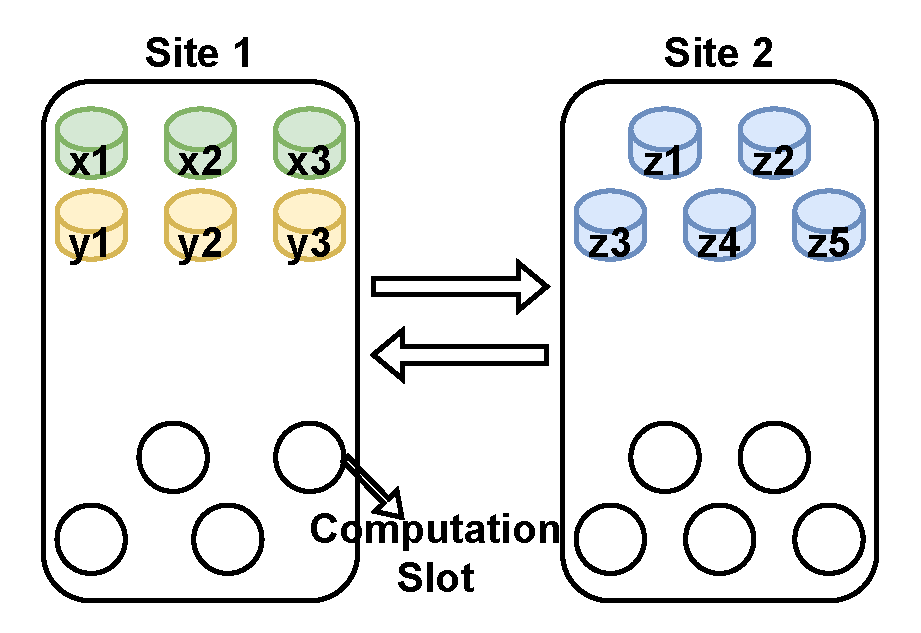
\includegraphics[width=\textwidth]{Image/Eg1.drawio.pdf}
    \caption{Initial system state}
    \label{Fg:eg1}
  \end{subfigure}
  \hfill
  \begin{subfigure}[t]{0.32\textwidth}
    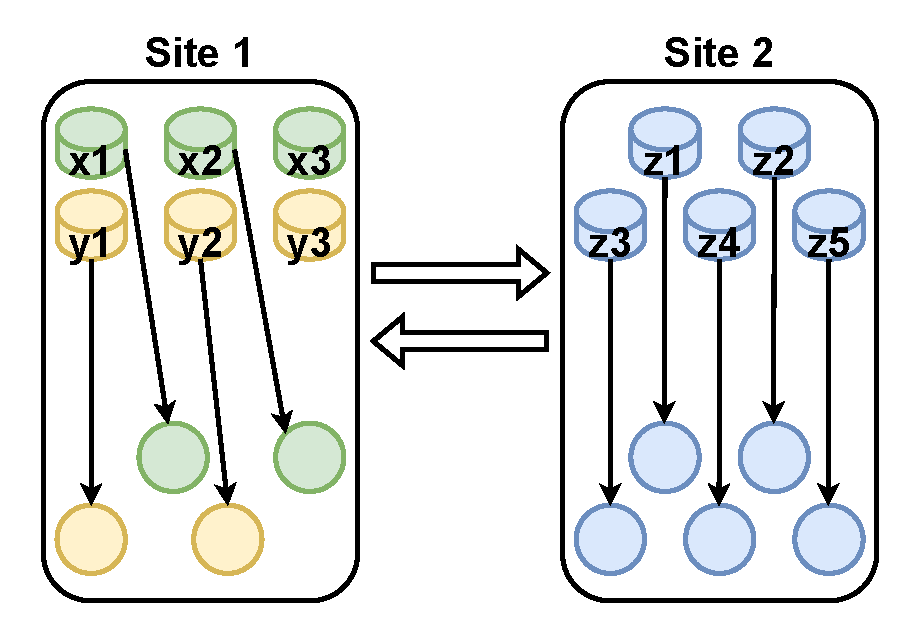
\includegraphics[width=\textwidth]{Image/Eg2.drawio.pdf}
    \caption{Fair allocation without transmission}
    \label{Fg:eg2}
  \end{subfigure}
  \hfill
  \begin{subfigure}[t]{0.32\textwidth}
    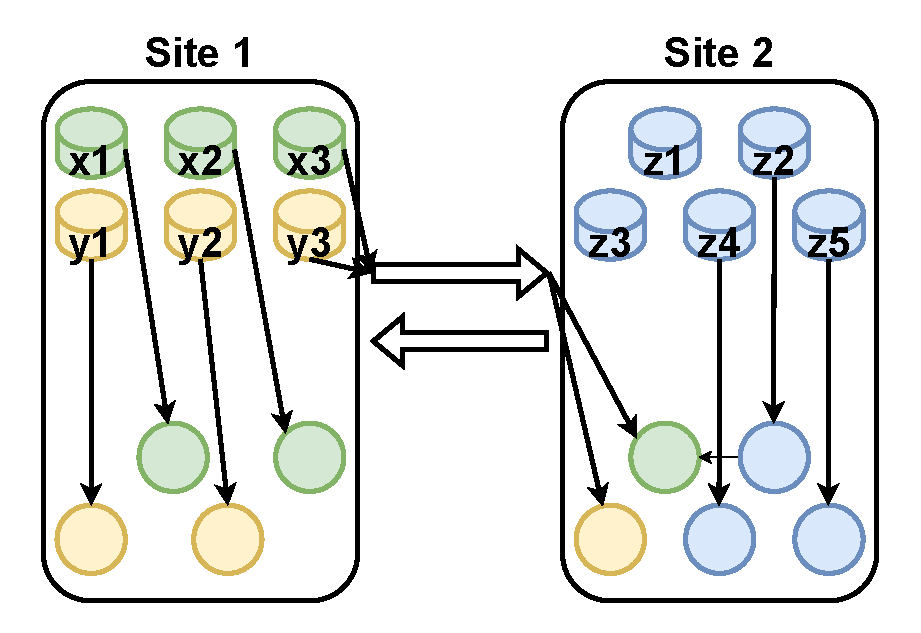
\includegraphics[width=\textwidth]{Image/Eg3.drawio.pdf}
    \caption{Fair allocation utilizing network resources}
    \label{Fg:eg3}
  \end{subfigure}
  \caption{An intuitive example}
  \label{fig:Motivation_eg}
\end{figure}

Figure \ref{fig:Motivation_eg} provides an example of the static problem to illustrate that transferring job demands can help improve the fairness of resource allocation. Suppose a geo-distributed system has 2 sites $S_1$ and $S_2$ with capacities of $4$ and $5$ computing slots respectively. There are three active jobs $x$, $y$ and $z$ in the system. As shown in Figure \ref{Fg:eg1}, jobs $x$ and $y$ have $3$ tasks each, where the input data is available on site $S_1$; job $z$ has $5$ tasks, where the input data is available on site $S_2$. If no demand can be transferred between sites, the most balanced resource allocation among jobs $x$, $y$ and $z$ is $2$, $2$ and $5$ computing slots as illustrated in Figure \ref{Fg:eg2}, because jobs $x$ and $y$ do not have demands on site $S_2$. With a transfer limit of $2$, we can transfer one task of job $x$ and one task of job $y$ from $S_1$ to $S_2$, and allocate them with computing slots on $S_2$. As a result, all jobs $x$, $y$ and $z$ are allocated $3$ computing slots each as shown in Figure \ref{Fg:eg3}, which is more balanced (fair) from the global perspective.


\section{Preliminaries}
\label{sec3:prelim}
\subsection{Max-min Fairness}
Max-Min Fairness (MMF) is one of the most common resource allocation strategies, which takes ``serving the most unsatisfied user'' as priority. Considering the resource allocation among $n$ jobs as an $n$-dimensional vector, MMF can be defined as follows \cite{radunovic2007unified}:

\begin{definition}
    \label{def:MMF}
    Consider a set $V$ of n-dimensional vectors. A vector $\vec x \in V$ is max-min fair on set $V$, if and only if for any $\vec y \in V$, if $y_s > x_s$ for an index $s \in \{1, 2, ..., n\}$, there must exist another index $t \in \{1, 2, ..., n\}$ such that $y_t < x_t \leq x_s$.
\end{definition}

Based on the above definition, if we want to increase a component $x_s$ in a max-min fair vector $\vec x$ while keeping the new vector staying in the vector set $V$, we must decrease another component $x_t$ in $\vec x$ whose original value is less than or equal to that of $x_s$. The max-min fair vector is unique if it exists, because if there are multiple max-min fair vectors within a given vector set $V$, we can derive contradiction simply by applying the definition of MMF to them. Clearly, the max-min fair vector does not exist in every vector set. Previous work has proved sufficient conditions for the existence of the max-min fair vector \cite{radunovic2007unified}. 
\begin{theorem}
    If a set $V$ is compact and convex, then it is max-min achievable.
\label{the:achievable}
\end{theorem}

\subsection{Aggregate Max-min Fairness}
A naive idea of applying MMF to distributed job execution is to consider each site independently and find the MMF resource allocation among jobs on each site based on their local demands. This policy is known as Independent Max-min Fairness (IMF) \cite{AMF}. However, IMF can be far away from providing fair services to jobs from the global perspective due to the possibly unbalanced distribution of job demands and compute capacities among sites.

Guan \textit{et al.} \cite{AMF} defined Aggregate Max-min Fairness (AMF) for distributed job execution and presented an algorithm to achieve AMF. AMF treats the distributed system as a united resource pool and constructs an aggregate allocation vector to represent each job's total resource allocation across all distributed sites: 
$$\vec{A} = \langle \sum_{j=1}^m a_{1j},  \sum_{j=1}^m a_{2j}, ..., \sum_{j=1}^m a_{nj} \rangle.$$
AMF requires this vector to be max-min fair among all possible aggregation vectors. While the AMF vector is unique if it exists, there may be multiple ways of resource allocation by sites to jobs producing this AMF vector since the vector only specifies each job's aggregate allocation across all sites. 

AMF does not consider utilizing network resources to transfer job demands between sites. Transferring job demands has the potential to improve the fairness of compute resource allocation for jobs as well as the system utility.

\section{Dynamic Aggregate Max-min Fairness}
\label{sec:DAMF}
We propose a new resource allocation policy called Dynamic Aggregate Max-min Fairness (DAMF) to improve the fairness of resource allocation by making use of network resources. Given the demand matrix, site capacities and transfer limits, there are a variety of possible transmission matrices and each would give rise to a number of feasible and rational allocations. Under this circumstance, DAMF requires the aggregate allocation vector to be max-min fair among all the vectors derived from the allocation matrices resulting from all possible transmission matrices. Let $\mathcal{X}$ be the set of all feasible and rational allocation matrices under all possible transmission matrices, and $X$ be the set of all aggregate allocation vectors drawn from $\mathcal{X}$. DAMF can be formally defined as follows:

\begin{definition}
    An allocation $A_{n*m}$ satisfies Dynamic Aggregate Max-min Fairness, if and only if its aggregate allocation vector $\vec A$ is max-min fair over the set $X$.
\end{definition}

We prove that DAMF exists by showing the compactness and convexity of set $X$. 
\begin{lemma}
    The set $X$ is compact.
\label{lem:compact}
\end{lemma}

\begin{proof}
Consider any aggregate allocation vector $\vec{A} = \langle\sum_{j=1}^m a_{1j}, \allowbreak $ $\sum_{j=1}^m a_{2j},\allowbreak \dots, \allowbreak \sum_{j=1}^m a_{nj}\rangle$ derived from some allocation matrix $A$ under some demand matrix $D + \Delta D$ after transmission. According to constraints (\ref{eq:allocfeas}), (\ref{eq:new_rational}) and (\ref{eq:trx2}), for the \textit{i}-th component $\sum_{j=1}^m a_{ij}$, we have $0 \leq \sum_{j=1}^m a_{ij} \leq \sum_{j=1}^m \min\{u_j, d_{ij} +\Delta d_{ij}\} \leq \sum_{j=1}^m \min\{u_j, d_{ij} +c_j\}$. Thus, the set $X$ is closed and bounded. Hence, it is compact.
\end{proof}

\begin{lemma}
    The set $X$ is convex.
\label{lem:convex}
\end{lemma}

\begin{proof}
Based on the definition of convexity, we need to prove that for any two vectors $\vec A, \vec B \in X$ and any $0 \leq \lambda \leq 1$, it holds that $\lambda \vec A + (1-\lambda) \vec B \in X$.

Let $\mathcal{T}$ be the set of all possible transmission matrices satisfying (\ref{eq:trx1}), (\ref{eq:trx2}) and (\ref{eq:trx3}). We first prove that $\mathcal{T}$ is convex. i.e., for any two transmission matrices $\Delta D,\Delta D' \in \mathcal{T}$ and any $0 \leq \lambda \leq 1$, $\lambda \cdot \Delta D + (1-\lambda) \cdot \Delta D' \in \mathcal{T}$.

Firstly, $\lambda \cdot \Delta D + (1-\lambda) \cdot \Delta D'$ satisfies constraint (\ref{eq:trx1}): since $\Delta D,\Delta D' \in \mathcal{T}$, for each job $J_i$ and each site $S_j$, we have $d_{ij} + \Delta d_{ij} \geq 0$ and $d_{ij} + \Delta d_{ij}' \geq 0$, and hence, 
\begin{align}
    \nonumber &d_{ij} + \lambda \cdot \Delta d_{ij} + (1-\lambda) \cdot \Delta d_{ij}'\\
    \nonumber &= \lambda \cdot (d_{ij} + \Delta d_{ij}) + (1-\lambda) \cdot (d_{ij} + \Delta d_{ij}')\\
    \nonumber &\geq \lambda\cdot 0+(1-\lambda)\cdot 0 =0. 
\end{align}

Similarly, it can be shown that $\lambda \cdot \Delta D + (1-\lambda) \cdot \Delta D'$ satisfies constraints (\ref{eq:trx2}) and (\ref{eq:trx3}). As a result, $\lambda \cdot \Delta D + (1-\lambda) \cdot \Delta D' \in \mathcal{T}$ and thus, $\mathcal{T}$ is a convex set.

Next, suppose the original demand matrix is $D$, and vector $\vec A$ and $\vec B$'s corresponding allocation and transmission matrices are $\{A, \Delta D^A\}$ and $\{B, \Delta D^B\}$, respectively. Since the set $\mathcal{T}$ is convex, we have $\lambda \cdot \Delta D^A + (1-\lambda) \cdot \Delta D^B \in \mathcal{T}$. By definition, $\lambda \vec A + (1-\lambda) \vec B$ is the aggregate allocation vector for the allocation matrix $\lambda A + (1-\lambda) B$. We prove that $\lambda A + (1-\lambda) B$ is a rational and feasible allocation matrix for the demand matrix $D + \lambda \cdot \Delta D^A + (1-\lambda) \cdot \Delta D^B$.

Since $A$ and $B$ are feasible, by constraint (\ref{eq:allocfeas}) we have
\begin{align}
    \forall j \in [m], \quad \nonumber\sum_{i=1}^n a_{ij} \leq u_j, \quad \nonumber\sum_{i=1}^n b_{ij} \leq u_j.
\end{align}
Thus,
\begin{align}
    \nonumber \sum_{i=1}^n\left(\lambda a_{ij} + (1-\lambda)b_{ij}\right) &\leq \lambda u_j+ (1-\lambda) u_j =u_j.
\end{align}
Hence, $\lambda A + (1-\lambda)B$ is feasible. Similarly, it can be shown that $\lambda A + (1-\lambda)B$ is rational. Therefore, $\lambda A + (1-\lambda)B \in \mathcal{X}$. As a result, $\lambda \vec A + (1-\lambda) \vec B \in X$, and $X$ is a convex set.
\end{proof}
Lemmas \ref{lem:compact} and \ref{lem:convex} together with Theorem \ref{the:achievable} give rise to the following conclusion:
\begin{theorem}
    Dynamic Aggregate Max-min Fairness is achievable.
\label{the:DAMFachievable}
\end{theorem}

\section{Properties of DAMF}
\label{sec:property}
In this section, we study whether DAMF satisfies the properties of Pareto efficiency, envy-freeness and strategy-proofness, which are well-accepted characteristics of fairness. %\sout{ and sharing incentive}.
\subsection{Pareto Efficiency}
Pareto efficiency means that no further improvement can be achieved which makes at least one individual better off without making any other individual worse off \cite{DRF}. This includes two aspects \cite{gutman2012GDF}: first, no resource required by any consumer is left idle; second, no consumer is allocated any resource that it does not need.

In our distributed job execution context, suppose the DAMF vector and its corresponding allocation matrix are $\vec A$ and $A_{n*m}$ respectively. Pareto efficiency means that for any other feasible and rational allocation matrix $A'_{n*m}$ and its corresponding aggregate allocation vector $\vec A'$, if there is an index $i$ such that the $i$-th component of $\vec A$ is larger than the $i$-th component of $\vec A'$, i.e., $\sum_{j=1}^m a'_{ij} > \sum_{j=1}^m a_{ij}$, there must be another index $k$ such that the $k$-th component of $\vec A$ is smaller than the $k$-th component of $\vec A'$, i.e., $\sum_{j=1}^m a'_{kj} < \sum_{j=1}^m a_{kj}$.

\begin{theorem}
    DAMF is Pareto efficient.
\end{theorem}
\begin{proof}
    By definition, the DAMF vector is the max-min fair vector among all possible aggregate allocation vectors under all possible transmission matrices. For any other feasible and rational allocation matrix $A'_{n*m}$ and its corresponding aggregate allocation vector $\vec A'$, if $\sum_{j=1}^m a'_{ij} > \sum_{j=1}^m a_{ij}$ for some job $J_i$, then based on Definition \ref{def:MMF}, there exists another job $J_k$ such that $\sum_{j=1}^m a'_{kj} < \sum_{j=1}^m a_{kj} \leq \sum_{j=1}^m a_{ij}$. Hence, the theorem is proven. 
\end{proof}

\subsection{Envy-freeness}
Envy-freeness means that no individual would envy another individual's allocation. More specifically, in our distributed job execution context, envy-freeness means that for any job $J_l$, its usable allocation will not increase if it is given any other job $J_k$'s transmission and allocation.

\begin{theorem}
    DAMF is envy-free.
\end{theorem}

\begin{proof}
Let $\vec A$ be the DAMF vector, and $A_{n*m}$, $\Delta D_{n*m}$ be its corresponding allocation and transmission matrices respectively.
Assume on the contrary that they are not envy-free, that is, a job $J_l$ will have its usable allocation increased if it is given another job $J_k$'s transmission $\Delta d_{kj}$'s and allocation $a_{kj}$'s. Note that the transmission refers to the network bandwidth allocated, and $J_l$ does not have to fully utilize the allocated bandwidth in order to optimize its usable allocation. Let $r_{lj}$'s be the actual transmission used by $J_l$, where for each site $S_j$, $|r_{lj}| \leq |\Delta d_{kj}|$ (transmission is within the allocated bandwidth), $d_{lj} + r_{lj} \geq 0$ (transmission is feasible), and $\sum_{j=1}^m r_{lj} = 0$ (the overall demand of $J_l$ is unchanged after transmission). Then, the demands of $J_l$ on all sites would become $d_{lj} + r_{lj}$'s. Thus, $J_l$'s usable allocation on each site $S_j$ is $\min\{d_{lj}+r_{lj}, a_{kj}\}$. If $J_l$'s total usable allocation over all sites increases, it means that
$$
\sum_{j=1}^m \min\{d_{lj}+r_{lj}, a_{kj}\} > \sum_{j=1}^m a_{lj}.
$$
This implies two facts:

(i) By eliminating the $\min$ operator, we have
$$
\sum_{j=1}^m a_{kj} > \sum_{j=1}^m a_{lj},
$$
which means job $J_k$'s aggregate allocation is larger than $J_l$'s aggregate allocation in the DAMF vector.

(ii) There must be at least one site $S_{j'}$ such that $\min\{d_{lj'}+r_{lj'}, a_{kj'}\} > a_{lj'}$, which indicates $d_{lj'}+r_{lj'} > a_{lj'}$ and $a_{kj'} > a_{lj'}$. The former inequality means that $J_l$'s demand on site $S_{j'}$ is not completely satisfied, and the latter inequality means that $J_k$'s allocation on site $S_{j'}$ is larger than $J_l$'s allocation on $S_{j'}$. 

By (ii), from the DAMF allocation matrix $A_{n*m}$, we could increase $a_{lj'}$ by decreasing $a_{kj'}$ on site $S_{j'}$. Accordingly, $J_l$'s aggregate allocation increases while $J_k$'s aggregate allocation decreases. Note that by (i), $J_k$'s aggregate allocation is larger than $J_l$'s aggregate allocation in $A_{n*m}$. This implies that we can increase the $l$-th component of the DAMF vector $\vec A$ by decreasing its $k$-th component which is larger, and this contradicts the fact that $\vec A$ is the max-min fair vector among all possible aggregate allocation vectors.
\end{proof}

\subsection{Strategy-proofness}
Strategy-proofness means that no individual could achieve better allocation by lying about its demand. In our distributed job execution context, strategy-proofness requires that no job could get higher usable allocation by lying about its demand $d_{ij}$'s, even if this would cause the recomputation of the transmission matrix $\Delta D$ and the allocation matrix $A$.

\begin{theorem}
    DAMF is strategy-proof.
\end{theorem}

\begin{proof}
Let $\vec A$ be the DAMF vector, and $A_{n*m}$, $\Delta D_{n*m}$ be its corresponding allocation and transmission matrices derived from the true demand matrix $D_{n*m}$ (i.e., when all jobs are honest). Let $D'_{n*m}$ be the misclaimed demand matrix when a job $J_l$ lies about its demand, and $A'_{n*m}$ and $\Delta D'_{n*m}$ be the resultant allocation matrix and transmission matrix respectively. Note that the transmission refers to the network bandwidth allocated. $J_l$ does not have to fully utilize the allocated bandwidth in order to optimize its usable allocation. Let $r_{lj}$'s be the actual transmission used by $J_l$, where for each site $S_j$, $|r_{lj}| \leq |\Delta d'_{lj}|$ (transmission is within the allocated bandwidth), $d_{lj} + r_{lj} \geq 0$ (transmission is feasible for $J_l$'s true demand), and $\sum_{j=1}^m r_{lj} = 0$ (the overall demand of $J_l$ is unchanged after transmission). For notational convenience, we define $R$ as the transmission matrix actually used by all jobs, i.e., $R$ replaces $\Delta d'_{lj}$'s with $r_{lj}$'s for job $J_l$ and keeps all other elements unchanged in $\Delta D'$. Then, the real demand matrix after transmission is given by $D + R$. In particular, the real demands of $J_l$ at all sites are $d_{lj} + r_{lj}$'s. Thus, $J_l$'s usable allocation on each site $S_j$ is $\min\{d_{lj}+r_{lj}, a'_{lj}\}$. We prove that $J_l$'s total usable allocation over all sites cannot increase, i.e.,
$$
\sum_{j=1}^m \min\{d_{lj}+r_{lj}, a'_{lj}\} \leq \sum_{j=1}^m a_{lj}. 
$$

We prove it by contradiction. Assume on the contrary that $J_l$'s total usable allocation over all sites increases: 
\begin{equation}
\sum_{j=1}^m \min\{d_{lj}+r_{lj}, a'_{lj}\} > \sum_{j=1}^m a_{lj}.
\label{eq:strategy1}
\end{equation}
It follows that 
\begin{equation}
\sum_{j=1}^m a'_{lj} >\sum_{j=1}^m a_{lj}.
\label{eq:strategy4}
\end{equation}

Since $J_l$ lies, it is possible that it gets excessive allocation than its real demand on some sites. Next, we construct a rational allocation matrix $B'$ by shrinking $J_l$'s excessive allocation (if any) in $A'$ to its real demand:

(i) For each job $J_i \neq J_l$, let $b'_{ij} = a'_{ij}$. Since these jobs are honest about their demands, their allocations must be rational: 
$$\forall j \in [m], \quad b'_{ij} = a'_{ij} \leq d_{ij}+\Delta d'_{ij} = d_{ij}+ r_{ij}.$$

(ii) For job $J_l$, if its allocation $a'_{lj}$ on site $S_j$ does not exceed its real demand $d_{lj} + r_{lj}$, it is kept the same in $B'$:
$$\forall j \in[m] \text{~where~} a'_{lj} \leq d_{lj} + r_{lj}, \quad b'_{lj} = a'_{lj}.$$
    
(iii) For job $J_l$, if its allocation $a'_{lj}$ on site $S_j$ exceeds its real demand $d_{lj} + r_{lj}$, we shrink it to be the real demand in $B'$:
$$\forall j \in [m] \text{~where~} a'_{lj} > d_{lj} + r_{lj}, \quad b'_{lj} = d_{lj} + r_{lj}.$$

In short, $B'$ records the allocations in $A'$ that can be actually used by all jobs. It is clear that $B'$ is a feasible and rational allocation matrix given the real demand matrix $D + R$.
For simplicity, $B'$ can be uniformly written as follows:
$$
\forall i \in [n], j \in [m], \; b'_{ij} = \min\{d_{ij}+r_{ij}, a'_{ij}\}.
$$

It then follows from (\ref{eq:strategy1}) that
\begin{equation}
\sum_{j=1}^m b'_{lj} >\sum_{j=1}^m a_{lj},
\label{eq:strategy2}
\end{equation}
which means that $J_l$'s aggregate allocation increases from $A$ to $B'$.

By definition, $A$'s aggregate allocation vector $\vec A$ is the max-min fair vector over all possible allocation matrices including those under the real demand matrix $D + R$. Based on the definition of max-min fairness and (\ref{eq:strategy2}), there must be another job $J_{i_1}$ whose aggregate allocation in $A$ is no larger than $J_l$ and whose aggregate allocation decreases from $A$ to $B'$:
$$
\sum_{j=1}^m a_{lj} \geq \sum_{j=1}^m a_{i_1j} > \sum_{j=1}^m b'_{i_1j}.
$$

Clearly, $J_{i_1}$ is different from $J_l$. Thus, by the above construction, $J_{i_1}$'s allocations in $B'$ and $A'$ are the same. Hence, the inequality above can be rewritten as:
\begin{equation}
\sum_{j=1}^m a_{lj} \geq \sum_{j=1}^m a_{i_1j} > \sum_{j=1}^m a'_{i_1j}.
\label{eq:strategy3}
\end{equation}

Next, we construct another allocation matrix $B$ based on $A$ assuming that the demand matrix is $D'+R$ (which is the demand matrix used to derive $A'$): 

(i) For each job $J_i \neq J_l$, let $b_{ij} = a_{ij}$.

(ii) For job $J_l$, if its allocation $a_{ij}$ on site $S_j$ does not exceed the demand $d'_{lj}+r_{lj}$, it is kept the same in $B$: $b_{lj} = a_{lj}$.

(iii) For job $J_l$, if its allocation $a_{ij}$ on site $S_j$ exceeds the demand $d'_{lj} +r_{lj}$, we shrink it to be the latter demand in $B$: $b_{lj} = d'_{ij} +r_{ij}$.

In short, $B$ is built by shrinking $J_l$'s allocation in $A$ exceeding the demand in $D'+R$ to the latter:
$$
\forall i \in [n], j \in [m], \; b_{ij} = \min\{d'_{ij}+r_{ij}, a_{ij}\}.
$$

Since $J_{i_1}$ is different from $J_l$,  $J_{i_1}$'s allocations in $B$ and $A$ are the same: $\sum_{j=1}^m a_{i_1j} =\sum_{j=1}^m b_{i_1j}$. Together with (\ref{eq:strategy3}), it can be inferred that $J_{i_1}$'s aggregate allocation increases from $A'$ to $B$, \textit{i.e.}, 
\begin{equation}
\sum_{j=1}^m b_{i_1j} > \sum_{j=1}^m a'_{i_1j}.
\label{eq:strategy8}
\end{equation}

Note that both $A'$ and $B$ are based on the demand matrix $D' + R$ and are feasible and rational. By definition, the aggregate allocation vector of $A'$ is the max-min fair vector over all possible allocation matrices including those under the demand matrix $D' + R$. Since $J_{i_1}$'s aggregate allocation increases from $A'$ to $B$, based on the definition of max-min fairness, there must be another job $J_{i_2}$ whose aggregate allocation in $A'$ is no larger than $J_{i_1}$ and whose aggregate allocation decreases from $A'$ to $B$:
\begin{equation}
\sum_{j=1}^m a'_{i_1 j} \geq \sum_{j=1}^m a'_{i_2 j} > \sum_{j=1}^m b_{i_2 j}.
\label{eq:strategy5}
\end{equation}

Clearly, $J_{i_2}$ is different from $J_{i_1}$. In addition, by (\ref{eq:strategy4}), (\ref{eq:strategy3}) and (\ref{eq:strategy5}), we have
\begin{equation}
\sum_{j=1}^m a'_{l j} > \sum_{j=1}^m a'_{i_1 j} \geq \sum_{j=1}^m a'_{i_2 j}.
\label{eq:strategy0}
\end{equation}
Thus, $J_{i_2}$ is also different from $J_l$. Hence, $J_l$, $J_{i_1}$ and $J_{i_2}$ are three distinct jobs.

By the construction of $B$, $J_{i_2}$'s allocations in $B$ and $A$ are the same. Moreover, by the construction of $B'$, $J_{i_2}$'s allocations in $B'$ and $A'$ are also the same. Therefore, (\ref{eq:strategy5}) implies that:
\begin{equation}
\sum_{j=1}^m b'_{i_2 j} > \sum_{j=1}^m a_{i_2 j},
\label{eq:strategy6}
\end{equation}
which means that $J_{i_2}$'s aggregate allocation increases from $A$ to $B'$. 

Now we can repeat the above analysis. Similar to the argument following (\ref{eq:strategy2}), based on the definition of max-min fairness for $A$ and (\ref{eq:strategy6}), there must be another job $J_{i_3}$ whose aggregate allocation in $A$ is no larger than $J_{i_2}$ and whose aggregate allocation decreases from $A$ to $B'$:
$$
\sum_{j=1}^m a_{i_2j} \geq \sum_{j=1}^m a_{i_3j} > \sum_{j=1}^m b'_{i_3j}.
$$

Similarly, it can be shown that $J_{i_3}$ is different from any of the jobs $J_l$, $J_{i_1}$ and $J_{i_2}$. Since $J_{i_3}$ is different from $J_l$, its allocations keep the same from $A$ to $B$ and from $A'$ to $B'$. Therefore, $J_{i_3}$'s aggregate allocation increases from $A'$ to $B$:
\begin{equation}
\sum_{j=1}^m b_{i_3j} > \sum_{j=1}^m a'_{i_3j}.
\label{eq:strategy7}
\end{equation}

Then, similar to the argument following (\ref{eq:strategy8}), 
based on the definition of max-min fairness for $A'$ and (\ref{eq:strategy7}), there must be another job $J_{i_4}$ whose aggregate allocation in $A'$ is no larger than $J_{i_3}$ and whose aggregate allocation decreases from $A'$ to $B$:
$$
\sum_{j=1}^m a'_{i_3j} \geq \sum_{j=1}^m a'_{i_4j} > \sum_{j=1}^m b_{i_4j}.
$$

Similar to (\ref{eq:strategy0}), it can be shown that $J_{i_4}$ is different from any of the jobs $J_l$, $J_{i_1}$, $J_{i_2}$, $J_{i_3}$, and 
\begin{equation}
\sum_{j=1}^m a'_{l j} > \sum_{j=1}^m a'_{i_1 j} \geq \sum_{j=1}^m a'_{i_2 j} > \sum_{j=1}^m a'_{i_3 j} \geq \sum_{j=1}^m a'_{i_4 j}.
\label{eq:strategy9}
\end{equation}
Since $J_{i_4}$ is different from $J_l$, its allocations keep the same from $A$ to $B$ and from $A'$ to $B'$. Therefore, $J_{i_4}$'s aggregate allocation increases from $A$ to $B'$:
$$
\sum_{j=1}^m b'_{i_4j} > \sum_{j=1}^m a_{i_4j}.
$$

By repeating the above process continuously, we can obtain an infinite sequence of jobs $J_{i_1}, J_{i_2}, J_{i_3}, J_{i_4}, J_{i_5}, J_{i_6}, \dots$ with non-increasing aggregate allocations in $A'$ like (\ref{eq:strategy9}), which contradicts that there are a finite number of jobs. Hence, the theorem is proven.
\end{proof}

% 请确保在 LaTeX 文件的导言区（Preamble）引入了该宏包：
% \usepackage[linesnumbered,ruled,vlined]{algorithm2e}

\begin{algorithm}[htbp]
\caption{Computing DAMF Allocation}\label{alg:basic}

    % 1. 输入输出与初始化 (不再使用 \STATE)
    \KwIn{A set of sites $\{S_1, S_2, ..., S_m\}$ with capacities $\{u_1, u_2, \dots, u_m\}$ and transfer limits $\{c_1, c_2, \dots, c_m\}$; a set of jobs $\{J_1, J_2, \dots, J_n\}$ with data partition weights $\{w_1, w_2, \dots, w_n\}$ and demand matrix $D$}
    \KwOut{A DAMF allocation matrix $A$; a transmission matrix $\Delta D$}
    
    \BlankLine % 插入一个空行隔开初始化
    $A \leftarrow \textbf{0}$\;
    $\Delta D \leftarrow \textbf{0}$\;
    $\mathcal{J} \leftarrow \{J_1, J_2, ..., J_n\}$\;
    \BlankLine

    % 2. 主循环结构 (花括号包裹，删除了 \ENDWHILE)
    \While{$\mathcal{J} \neq \emptyset$}{
        Solve the following linear program:\;
        \quad Maximize $T$, subject to:\;
        \quad\quad $\forall J_i \in \mathcal{J} : \sum^m_{j=1}a_{ij} \geq T$\;
        \quad\quad $\forall J_i \notin \mathcal{J} : \sum^m_{j=1}a_{ij} = t_i$\;
        \quad\quad $\forall j \in [m]: \sum^n_{i=1}a_{ij} \leq u_j$\;
        \quad\quad $\forall i \in [n], j \in [m]: 0 \leq a_{ij} \leq d_{ij}+\Delta d_{ij}$\;
        \quad\quad $\forall j \in [m]: \sum_{i=1}^n |w_i\Delta d_{ij}| \leq c_j$\;
        \quad\quad $\forall i \in [n]: \space \sum_{j=1}^m \Delta d_{ij}=0$\;
        
        Let $T_{max}$ be the outcome of the above linear program\;
        \BlankLine
        
        % For 循环 (删除了 \ENDFOR)
        \For{each $J_l \in \mathcal{J}$}{
            % If - Else If 结构 (\Eclif) 
            \eIf{$\sum^m_{j=1} d_{lj} = T_{max}$}{
                $t_l \leftarrow T_{max}$\;
                $\mathcal{J} \leftarrow \mathcal{J} \setminus\{J_l\}$\;
            }{
                \If{$\sum^m_{j=1} a_{lj}= T_{max} \text{ and } (\forall j \in [m], a_{lj} = d_{lj} \lor \sum^n_{i=1}a_{ij}=u_j)$}{
                    Check the feasibility of the following program:\;
                    \quad $\sum_{j=1}^n a_{lj} > T_{max}$\;
                    \quad $\forall J_i \in \mathcal{J} \land i \neq l: \sum^m_{j=1}a_{ij}=T_{max}$\;
                    \quad $\forall J_i \notin \mathcal{J} : \sum^m_{j=1}a_{ij}=t_i$\;
                    \quad $\forall j \in [m]: \sum^n_{i=1}a_{ij} \leq u_j$\;
                    \quad $\forall i \in [n], j \in [m]: 0 \leq a_{ij} \leq d_{ij}+\Delta d_{ij}$\;
                    \quad $\forall j \in [m]: \sum_{i=1}^n |w_i\Delta d_{ij}| \leq c_j$\;
                    \quad $\forall i \in [n]: \space \sum_{j=1}^m \Delta d_{ij}=0$\;
                    \BlankLine
                    
                    \If{the above program is infeasible}{
                        $t_l \leftarrow T_{max}$\;
                        $\mathcal{J} \leftarrow \mathcal{J} \setminus\{J_l\}$\;
                    }
                }
            }
        }
    }
    \BlankLine
    \Return $A_{n \times m}, \Delta D_{n \times m}$\;
\end{algorithm}

% \section{Achieving DAMF}
% \label{sec:algo}
% \subsection{Algorithm for Computing DAMF Allocation}

% \begin{algorithm}[htbp]
% \caption{Computing DAMF Allocation}\label{alg:basic}
% \begin{algorithmic}[1]

% \STATE \textbf{Input}: A set of sites $\{S_1, S_2, ..., S_m\}$ with capacities and transfer limits $\{c_1, c_2, \dots, c_j\}$; a set of jobs $\{J_1, J_2, ..., J_n\}$ with demand matrix $D$; 
% \STATE \textbf{Output}: A DAMF allocation matrix $A$; a transmission matrix $\Delta D$;
% \STATE \textbf{Initialization}: $A \leftarrow \textbf{0}$; $\Delta D \leftarrow \textbf{0}$; $\mathcal{J} \leftarrow \{J_1, J_2, ..., J_n\}$;

% \WHILE{$\mathcal{J} \neq \emptyset$}
%     \STATE Solve the following linear program:
%     \STATE \quad Maximize $T$, subject to: 
%     \STATE \quad $\forall J_i \in \mathcal{J} : \sum^m_{j=1}a_{ij} \geq T$;
%     \STATE \quad $\forall J_i \notin \mathcal{J} : \sum^m_{j=1}a_{ij} = t_i$;
%     \STATE \quad $\forall j \in [m]: \sum^n_{i=1}a_{ij} \leq u_j$;
%     \STATE \quad $\forall i \in [n], j \in [m]: 0 \leq a_{ij} \leq d_{ij}+\Delta d_{ij}$;
%     \STATE \quad $\forall j \in [m]: \sum_{i=1}^n |\Delta d_{ij}| \leq c_j$;
%     \STATE \quad $\forall i \in [n]: \space \sum_{j=1}^m \Delta d_{ij}=0$;
%     \STATE Let $T_{max}$ be the outcome of the above linear program;
    
%     \FOR{each $J_l \in \mathcal{J} $}
%         \IF{$\sum^m_{j=1} d_{lj} = T_{max}$}
%             \STATE $t_l \leftarrow T_{max}$;
%             \STATE $\mathcal{J} \leftarrow \mathcal{J} \setminus\{J_l\}$; 
%         \ELSIF{$\sum^m_{j=1} a_{lj}= T_{max} \text{ and } (\forall j \in [m], a_{lj} = d_{lj} \lor \sum^n_{i=1}a_{ij}=u_j)$}
%             \STATE Check the feasibility of the following program:
%             \STATE \quad $\sum_{j=1}^n a_{lj} > T_{max}$;
%             \STATE \quad $\forall J_i \in \mathcal{J} \land i \neq l: \sum^m_{j=1}a_{ij}=T_{max}$;
%             \STATE \quad $\forall J_i \notin \mathcal{J} : \sum^m_{j=1}a_{ij}=t_i$;
%             \STATE \quad $\forall j \in [m]: \sum^n_{i=1}a_{ij} \leq u_j$;
%             \STATE \quad $\forall i \in [n], j \in [m]: 0 \leq a_{ij} \leq d_{ij}+\Delta d_{ij}$;
%             \STATE \quad $\forall j \in [m]: \sum_{i=1}^n |\Delta d_{ij}| \leq c_j$;
%             \STATE \quad $\forall i \in [n]: \space \sum_{j=1}^m \Delta d_{ij}=0$;
            
%             \IF{the above program is infeasible}
%                 \STATE $t_l \leftarrow T_{max}$;
%                 \STATE $\mathcal{J} \leftarrow \mathcal{J} \setminus\{J_l\}$;
%             \ENDIF
%         \ENDIF
%     \ENDFOR
% \ENDWHILE

% \STATE \textbf{return} $A_{n \times m}, \Delta D_{n \times m}$;
% \end{algorithmic}
% \end{algorithm}

We now design an iterative algorithm (Algorithm \ref{alg:basic}) to compute the DAMF allocation, inspired by the max-min programming method from \cite{radunovic2007unified} which can find the max-min fair allocation vector for any max-min achievable set. The basic idea is to simultaneously increase the allocations of all jobs. Once a job's demand is completely satisfied, the algorithm fixes its allocation and continues to increase the allocations of other jobs. The algorithm terminates when all job demands are satisfied or all available resources are used up.

Each iteration of our algorithm consists of two stages. In stage 1, we define a unified lower bound $T$ and maximize it by increasing the aggregate allocations of all jobs in set $\mathcal{J}$ simultaneously, where $\mathcal{J}$ is the set of jobs whose aggregate allocations have not been fixed yet. Initially, $\mathcal{J}$ contains all jobs (line 3). The maximum $T$ value is derived by solving a linear program which models the constraints of resource allocation introduced in Section \ref{sec:model_1} (lines 5-12), where $t_i$ is the aggregate allocation of a job $J_i$ that has been fixed. 

Let $T_{max}$ denote the maximum $T$ value obtained in stage~1. In stage 2, we identify jobs whose aggregate allocations are to be fixed. If a job $J_l$'s total demand is equal to $T_{max}$ amount of resources, it is fully satisfied. Thus, the algorithm fixes its aggregate allocation to be $T_{max}$ and removes it from $\mathcal{J}$ (lines 15-17). Otherwise, the algorithm checks whether it is possible to increase $J_l$'s aggregate allocation beyond $T_{max}$ without violating other jobs' allocations. If $J_l$'s aggregate allocation from stage 1 is already larger than $T_{max}$, or there exists a site on which $J_l$'s demand is not fully satisfied and the site has spare capacity (i.e., the condition in line 18 is not satisfied), clearly $J_l$'s aggregate allocation can be further increased. Otherwise, we change the aggregate allocation constraints for $J_l$ and other jobs by replacing "$\geq$" with "$>$" (line 20) and "$=$" (line 21) respectively, and then check whether the new linear program has any feasible solution (lines 19-26). If so, it implies that $J_l$'s allocation can be increased and $J_l$ will be kept in set $\mathcal{J}$. Otherwise, $J_l$'s aggregate allocation is fixed at $T_{max}$ and $J_l$ is removed from set $\mathcal{J}$ (lines 27-29). Note that this $T_{max}$ value is the aggregate resource amount, which means that $J_l$'s allocations on individual sites could vary in subsequent iterations as long as the aggregate amount is kept. The algorithm terminates when $\mathcal{J}$ becomes empty (line 4).

The linear program in Algorithm \ref{alg:basic} has $2mn$ variables and $2m+2n+mn$ constraints, where $m$ and $n$ are the numbers of sites and jobs respectively. Since there can be up to $n$ iterations and each iteration needs to solve up to $n$ linear programs in stage 2, the worst-case time complexity of Algorithm \ref{alg:basic} is $O(n^2*LP(2mn,2m+2n+mn))$, where $LP(2mn,2m+2n+mn)$ is the complexity for solving a linear program with $2mn$ variables and $2m+2n+mn$ constraints. 

\subsection{A Fast Approximation}
Algorithm 1 computes an exact DAMF allocation. However, its complexity could raise concern since solving large-scale linear programs can
be computationally expensive \cite{complexity_lip}. In this section, we propose a heuristic algorithm to derive a near-DAMF allocation with significantly reduced time complexity to enhance the practicality.

% 请确保在 LaTeX 文件的导言区（Preamble）引入了该宏包：
% \usepackage[linesnumbered,ruled,vlined]{algorithm2e}

\begin{algorithm}[htbp]
\caption{Heuristic to Approximate DAMF Allocation}\label{alg:approx}

    % 1. 输入输出与初始化
    \KwIn{A set of sites $\{S_1, S_2, ..., S_m\}$ with capacities $\{u_1, u_2, \dots, u_m\}$ and transfer limits $\{c_1, c_2, \dots, c_m\}$; a set of jobs $\{J_1, J_2, \dots, J_n\}$ with data partition weights $\{w_1, w_2, \dots, w_n\}$ and demand matrix $D$;}
    \KwOut{An allocation matrix $A$; a transmission matrix $\Delta D$;}
    
    \BlankLine
    $A = \textbf{0}$\;
    $\Delta D = \textbf{0}$\;
    $\vec{p} = \textbf{0}$\;
    Sort all sites in increasing order of the number of jobs with demands on each site (i.e., the cardinality of $\{J_i: a_{ij} > 0\}$)\; 
    \BlankLine

    % 2. 第一层嵌套 For 循环
    \For{each site $S_j$ in the sorted order}{
        Compute max-min fair allocation $\langle a_{1j}, a_{2j}, ..., a_{nj}\rangle$ on $S_j$ based on job demands $\{d_{1j}, d_{2j}, ..., d_{nj}\}$, capacity $u_j$ of $S_j$, and current aggregate allocation vector $\vec{p} = \langle p_{1}, p_{2}, ..., p_{n}\rangle$ as described in the main text\;
        
        \For{$i \in [n]$}{
            $p_i = p_i + a_{ij}$\;
        }
    }
    \BlankLine
    
    % 3. 集合赋值
    $\mathcal{S}_{spare} = \{ S_j~|~ \sum_{i=1}^n a_{ij} < u_j\}$\;
    $\mathcal{S}_{full} = \{ S_j~|~ \sum_{i=1}^n d_{ij} > u_j\}$\;
    $\mathcal{J} = \{ J_i~|~ \sum_{j=1}^m d_{ij} > \sum_{j=1}^m a_{ij}\}$\;
    \BlankLine

    % 4. 双层嵌套 While 循环
    \While{$\mathcal{S}_{spare} \neq \emptyset \land \mathcal{S}_{full} \neq \emptyset \land \mathcal{J} \neq \emptyset$}{
        Remove all $S_l$'s from $\mathcal{S}_{spare}$ and $\mathcal{S}_{full}$ that $c_l \le \min_{1\le i \le n}{w_i}$ or $\sum_{i=1}^n (d_{il} + \Delta d_{il}) = u_l$\;
        
        \While{$\mathcal{J} \neq \emptyset$}{
            Select job $J_x \in \mathcal{J}$ with the least aggregate allocation\;
            
            \eIf{$\forall S_j \in \mathcal{S}_{full}, d_{xj} + \Delta d_{xj} \leq a_{xj}$}{
                Remove $J_x$ from $\mathcal{J}$\;
            }{
                Select a site $S_y \in \mathcal{S}_{full}$ where $d_{xy} + \Delta d_{xy}> a_{xy}$\; 
                Select a site $S_z \in \mathcal{S}_{spare}$\;
                $\Delta d_{xy} = \Delta d_{xy} - 1$\;
                $\Delta d_{xz} = \Delta d_{xz} + 1$\;
                $a_{xz} = a_{xz} + 1$\;
                $c_y = c_y - w_x$\;
                $c_z = c_z - w_x$\;
                \break
            }
        }
    }
    \BlankLine
    \Return $A_{n*m}, \Delta D_{n*m}$\;
\end{algorithm}

% \begin{algorithm}[htbp]
% \caption{Heuristic to Approximate DAMF Allocation}\label{alg:approx}
% \begin{algorithmic}[1]

% \STATE \textbf{Input}: A set of sites $\{S_1, S_2, ..., S_m\}$ with capacities and transfer limits; a set of jobs $\{J_1, J_2, ..., J_n\}$ with demand matrix $D$;
% \STATE \textbf{Output}: An allocation matrix $A$; a transmission matrix $\Delta D$;
% \STATE \textbf{Initialization}: $A = \textbf{0}$; $\Delta D = \textbf{0}$; $\vec{p} = \textbf{0}$; sort all sites in increasing order of the number of jobs with demands on each site (i.e., the cardinality of $\{J_i: a_{ij} > 0\}$); 
% \FOR{each site $S_j$ in the sorted order}
% \STATE Compute max-min fair allocation $\langle a_{1j}, a_{2j}, ..., a_{nj}\rangle$
% on $S_j$ based on job demands $\{d_{1j}, d_{2j}, ..., d_{nj}\}$, capacity $u_j$ of $S_j$, and current aggregate allocation vector $\vec{p} = \langle p_{1}, p_{2}, ..., p_{n}\rangle$ as described in the main text;
% \FOR {$i \in [n]$}
% \STATE $p_i = p_i + a_{ij}$;
% \ENDFOR
% \ENDFOR
% \STATE $\mathcal{S}_{spare} = \{ S_j~|~ \sum_{i=1}^n a_{ij} < u_j\}$;
% \STATE $\mathcal{S}_{full} = \{ S_j~|~ \sum_{i=1}^n d_{ij} > u_j\}$;
% \STATE $\mathcal{J} = \{ J_i~|~ \sum_{j=1}^m d_{ij} > \sum_{j=1}^m a_{ij}\}$;
% \WHILE{$\mathcal{S}_{spare} \neq \emptyset \land \mathcal{S}_{full} \neq \emptyset \land \mathcal{J} \neq \emptyset$}
%     \STATE Remove all $S_l$'s from $\mathcal{S}_{spare}$ and $\mathcal{S}_{full}$ that $c_l = 0$ or $\sum_{i=1}^n (d_{il} + \Delta d_{il}) = u_l$;
% \WHILE{$\mathcal{J} \neq \emptyset$}
% \STATE Select job $J_x \in \mathcal{J}$ with the least aggregate allocation;
% \IF{$\forall S_j \in \mathcal{S}_{full}, d_{xj} + \Delta d_{xj} \leq a_{xj}$}
% \STATE Remove $J_x$ from $\mathcal{J}$;
% \ELSE
% \STATE Select a site $S_y \in \mathcal{S}_{full}$ where $d_{xy} + \Delta d_{xy}> a_{xy}$; 
% \STATE Select a site $S_z \in \mathcal{S}_{spare}$;
% \STATE $\Delta d_{xy} = \Delta d_{xy} - 1$;
% \STATE $\Delta d_{xz} = \Delta d_{xz} + 1$;
% \STATE $a_{xz} = a_{xz} + 1$;
% \STATE $c_y = c_y - 1$;
% \STATE $c_z = c_z - 1$;
% \STATE Break;
% \ENDIF
% \ENDWHILE
% \ENDWHILE
% \STATE \textbf{return} $A_{n*m}, \Delta D_{n*m}$
% \end{algorithmic}
% \end{algorithm}

The heuristic algorithm (Algorithm \ref{alg:approx}) proceeds in two steps. In step 1 (lines 4-9), we find a fast approximation to AMF (i.e., without transferring job demands between sites) in an iterative manner. Each iteration calculates the compute resource allocation for one site $S_j$, given the job demands and compute capacity on this site as well as the aggregate allocation vector $\vec p$ over the sites that have been processed in previous iterations (line 5). Suppose there are $n$ jobs running in the system. Let $\vec p = \langle p_{1}, p_{2}, ..., p_{n}\rangle$ be the current aggregate allocation vector and $\langle d_{1j}, d_{2j}, ..., d_{nj}\rangle$ be the job demands on site $S_j$. We would like to compute an allocation $\langle a_{1j}, a_{2j}, ..., a_{nj}\rangle$ on $S_j$ so that $\langle p_{1}+a_{1j}, p_{2}+a_{2j}, ..., p_{n}+a_{nj}\rangle$ is max-min fair among all possible allocations for the given $\vec p$. If the total demand of all jobs on site $S_j$ is no larger than its capacity, i.e., $\sum_{i=1}^n d_{ij} \leq u_j$, we can simply satisfy the demands of all jobs by setting $a_{ij} = d_{ij}$ for all $i$'s. Otherwise, we sort the jobs in increasing order of $p_{i}$, i.e., $p_{1} \leq p_{2} \leq ... \leq p_{n}$, and the resources on site $S_j$ will be allocated to a prefix of this job sequence by the definition of max-min fairness. If resources are allocated to the first $k$ jobs, the total resources allocated must be no more than 
\begin{equation}
\sum_{i=1}^k \left(\min\{p_{k+1}, p_i+d_{ij}\} - p_i\right),
\label{eq:waterfill}
\end{equation}
because the aggregate resource allocation of each job cannot exceed the given allocation $p_{k+1}$ of the next job ($(k+1)$-th job). Since (\ref{eq:waterfill}) is non-decreasing with $k$, we can use a binary search to find out which jobs will receive resource allocations on $S_j$ to make full use of its capacity $u_j$. After deciding $k$, we solve the equation $\sum_{i=1}^k \left(\min\{C, p_i+d_{ij}\} - p_i\right) = u_j$ to find out the maximum aggregate resource allocation $C$ among these jobs to achieve max-min fairness. Then, the $i$-th job will be allocated $a_{ij} = \min\{C, p_i+d_{ij}\} - p_i$ amount of resources. Apparently, the iterating order of sites has an impact on the final allocation result. Our idea is to sort all sites in increasing order of the number of jobs with demands on the site (line 3). A site demanded by more jobs is considered to have higher potential in balancing the final aggregate allocation, so we process it in a later iteration.

In step 2 (lines 10-30), we utilize the network resources to improve the allocation derived in step 1. It is not difficult to see that there exists a DAMF allocation (represented by a pair of transmission and allocation matrices) such that for every demand unit (one task) transferred, (i) the task involved is allocated compute resources at the destination site; and (ii) the compute resources at the source site are fully allocated. In fact, if a demand unit transferred does not satisfy (i), the transfer can be canceled without affecting the allocation matrix. Similarly, the transfer of a demand unit that violates (ii) can also be canceled and the task can be satisfied by compute resources at the source site. This would increase the compute resource allocation of the job involved without affecting the compute resource allocation of any other job, thereby contradicting that the original allocation is max-min fair.

Based on the observation above, we define two sets $\mathcal{S}_{spare}$ and $\mathcal{S}_{full}$ to record sites with spare capacities and with more job demands than capacities (lines 10-11), and a set $\mathcal{J}$ to record jobs whose demands are not fully satisfied (line 12). Then, we start a loop to transfer job demands from $\mathcal{S}_{full}$ sites to $\mathcal{S}_{spare}$ sites until either $\mathcal{S}_{spare}$, $\mathcal{S}_{full}$ or $\mathcal{J}$ becomes empty (which implies that no further improvement to the allocation can be made). To make effective use of network resources, we would like all job demands transferred to get compute resource allocations at destination sites. Intuitively, a site will not need to participate in transmissions if its bandwidth is used up or its updated local demand equals its capacity. Thus, within the loop, we first remove all such sites from $\mathcal{S}_{spare}$ and $\mathcal{S}_{full}$ (line 14). As a heuristic to approximate max-min fairness, among all jobs whose demands are not completely satisfied, we pick the job $J_x$ with the least aggregate allocation currently (line 16). If $J_x$'s demands are satisfied on all sites in $\mathcal{S}_{full}$ (implying that $J_x$'s unsatisfied demands locates at the sites that have been removed because no more bandwidth is available), we discard $J_x$ and examine the next job with the least aggregate allocation for demand transmission (lines 17-18). Otherwise, we select the source site and destination site for a transfer of $J_x$: the source site can be any site in $\mathcal{S}_{full}$ where $J_x$'s demand is not fully satisfied (line 20), and the destination site can be any site in $\mathcal{S}_{spare}$ (line 21). After deciding a transmission, we update the related matrices and remaining transfer limits (lines 22-26).

The heuristic algorithm does not require solving linear programs and has much lower time complexity. In step 1, it solves $m$ allocation problems separately (where $m$ is the number of sites). In the water-filling-like strategy, sorting takes $O(n \log n)$ time (where $n$ is the number of jobs), and the binary search takes $O(n \log n)$ time as computing (\ref{eq:waterfill}) takes $O(n)$ time. So, the time complexity of each iteration is $O(n \log n)$, and the total time complexity of step 1 is $O(m n \log n)$. In step 2, the algorithm transfers at most $cm/2 = O(m)$ units of job demand (assuming the transfer limits of all sites are a constant $c$). Updating $\mathcal{S}_{spare}$ and $\mathcal{S}_{full}$ takes $O(m)$ time. If we arrange all unsatisfied jobs in $\mathcal{J}$ as a min-heap based on their aggregate allocations, selecting the unsatisfied job with the least aggregate allocation takes $O(1)$ time. Selecting the source and destination sites takes $O(m)$ time. After the demand transfer, updating the min-heap of $\mathcal{J}$ takes $O(\log n)$ time.
Thus, each unit of demand transfer takes $O(m+\log n)$ time. If a source site for the selected job can always be found, the time complexity of step 2 is $O(m(m+\log n))$. If the selected job fails to find a source site for transmission, the job is discarded and updating the min-heap of $\mathcal{J}$ takes $O(\log n)$ time. In the worst case, discarding all such jobs incur a time complexity of $O(n (m + \log n))$. Therefore, the worst-case time complexity of step 2 is $O((m+n) (m+\log n))$. Hence, the overall complexity of the algorithm is $O(m n \log n + m^2)$. In the experiments, we shall empirically evaluate and compare the computation times of Algorithms \ref{alg:basic} and \ref{alg:approx}.

\subsection{Optimizing Job Completion Times}
In addition to providing fair resource allocation from the global perspective, we can further optimize the job completion times. The key idea is that DAMF fixes only the aggregate resource allocation for each job, while the particular allocations at individual sites can still be adjusted. In this case, the completion time of a job can be optimized by assigning the allocation proportionally to its demand at each site. For example, if a job has $2$ and $4$ tasks at two sites respectively and its aggregate allocation by DAMF is $3$ computing slots, then its allocations at the two sites can be set to $1$ and $2$ computing slots, so that the two sites can finish processing their tasks at the same time (to minimize job completion time) if all tasks have the same processing time. Meanwhile, we need to ensure that other jobs can also achieve their DAMF aggregate allocations. The details of our algorithm are shown in Algorithm \ref{alg:qos}.

% 请确保在 LaTeX 文件的导言区（Preamble）引入了该宏包：
% \usepackage[linesnumbered,ruled,vlined]{algorithm2e}

\begin{algorithm}[htbp]
\caption{Optimizing Job Completion Times}\label{alg:qos}

    % 1. 输入输出
    \KwIn{A set of sites $\{S_1, S_2, ..., S_m\}$ with capacities; a set of jobs $\{J_1, J_2, ..., J_n\}$ with demand matrix $D$; the aggregate allocation $e_i$ of each job $J_i$ in a DAMF allocation with corresponding transmission matrix $\Delta D$}
    \KwOut{An optimized allocation matrix $A'$}
    \BlankLine

    % 2. 外层 For 循环
    \For{$k = 1, 2, \dots, n$}{
        Solve the following linear program:\;
        Maximize $y_k$, subject to:\;
        \quad $\forall j \in [m], \sum_{i=1}^n a_{ij} \leq u_j$\;
        \quad $\forall i < k, j \in [m]: a_{ij} = a'_{ij}$\;
        \quad $\forall i \ge k, j \in [m]: 0 \le a_{ij} \le d_{ij}+\Delta d_{ij}$\;
        \quad $\forall i\ge k: \sum_{j=1}^m a_{ij} = e_i$\;
        \quad $\forall j \in [m]: a_{kj} = d_{kj}*y_k+z_{kj}$, $y_k \ge 0$, $z_{kj} \ge 0$\;
        \BlankLine
        
        % 3. 内层 For 循环
        \For{each $j\in[m]$}{
            $a'_{kj} \leftarrow a_{kj}$\;
        }
    }
    \BlankLine
    \Return $A'_{n*m}$\;
\end{algorithm}

% \begin{algorithm}[htbp]
% \caption{Optimizing Job Completion Times}
% \label{alg:qos}
% \begin{algorithmic}[1]

% \STATE \textbf{Input}: A set of sites $\{S_1, S_2, ..., S_m\}$ with capacities; a set of jobs $\{J_1, J_2, ..., J_n\}$ with demand matrix $D$; the aggregate allocation $e_i$ of each job $J_i$ in a DAMF allocation with corresponding transmission matrix $\Delta D$;
% \STATE \textbf{Output}: An optimized allocation matrix $A'$;

% \FOR{$k = 1, 2, \dots, n$}
% \STATE Solve the following linear program:
% \STATE Maximize $y_k$, subject to:
% \STATE \quad $\forall j \in [m], \sum_{i=1}^n a_{ij} \leq u_j$;
% \STATE \quad $\forall i < k, j \in [m]: a_{ij} = a'_{ij}$;
% \STATE \quad $\forall i \ge k, j \in [m]: 0 \le a_{ij} \le d_{ij}+\Delta d_{ij}$;
% \STATE \quad $\forall i\ge k: \sum_{j=1}^m a_{ij} = e_i$;
% \STATE \quad $\forall j \in [m]: a_{kj} = d_{kj}*y_k+z_{kj}$, \;$ y_k \ge 0$, $z_{kj} \ge 0$;
% \FOR{each $j\in[m]$}
% \STATE $a'_{kj} \leftarrow a_{kj}$;
% \ENDFOR
% \ENDFOR
% \STATE \textbf{return} $A'_{n*m}$.
% \end{algorithmic}
% \end{algorithm}

Algorithm \ref{alg:qos} optimizes the completion times of jobs iteratively from $J_1$ to $J_n$. In each iteration, the algorithm solves a linear program (lines 4-10) to optimize the completion time of a job $J_k$. The first constraint of the linear program (line 6) ensures that the allocations are feasible. The second constraint (line 7) retains the allocations of jobs already optimized. The third constraint (line 8) ensures that the allocations of remaining jobs are rational given the input transmission matrix. The fourth constraint (line 9) guarantees that the aggregate allocations of these jobs comply with DAMF. The last constraint (line 10) expresses $J_k$'s allocation $a_{kj}$ at each site $S_j$ as a linear combination $d_{kj}*y_k +z_{kj}$, where $y_k$ is a shared proportional coefficient for all sites and $z_{kj}$ is an auxiliary variable. Thus, by maximizing $y_k$, the resource allocation $a_{kj}$ across sites can be made as close to proportional as possible to the resource demand $d_{kj} + \Delta d_{kj}$ at each site, thereby minimizing job $J_k$'s completion time. After solving the linear program, $J_k$'s allocation at each site is decided and recorded in $A'$ (lines 11-13). Finally, the algorithm returns the optimized allocation $A'$ after all iterations. The set of jobs $\{J_1, J_2, ..., J_n\}$ input to the algorithm can be arranged in different orders based on job arrival times, job priorities, job demands, etc. In this paper, we sort the jobs based on their total demands from low to high so that jobs with smaller numbers of tasks are optimized earlier.

\subsection{Deployment}
\begin{figure}[t]
    \centering
    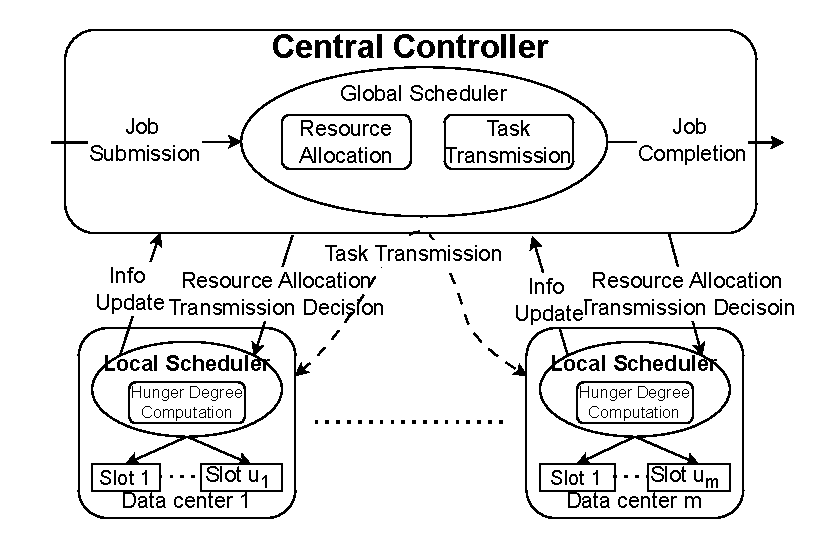
\includegraphics[width=0.7\linewidth]{Image/DAMF.drawio.pdf}
    \caption{System Architecture}
    \label{fig:Architecture}
\end{figure}

Algorithms \ref{alg:basic} and \ref{alg:approx} in the above sections derive a DAMF or near-DAMF resource allocation among active jobs at a snapshot of the system. In this section, we discuss how to apply them to online scenarios where jobs arrive dynamically for execution. As shown in Figure \ref{fig:Architecture}, the algorithm for computing the DAMF allocation can be deployed at a central scheduler of the distributed job execution system. The scheduler tracks the real-time resource capacities of the sites and the distributed demands of each job on all sites. Once an allocation is derived, the scheduler propagates the transmission matrix $\Delta D$ and the allocation matrix $A$ to relevant sites, where job demands (task input data) would be transferred based on $\Delta D$. The compute resource allocation at each site would follow the allocation matrix $A$. If the demand of a job on a site is larger than its allocation on the site, some of its tasks will have to wait. When a computing slot becomes available on a site, the site computes the "Hunger Degree" for jobs with pending tasks locally and selects the job with the lowest Hunger Degree to launch its task in the available slot. More specifically, the Hunger Degree of a job on a site is the ratio between the number of its tasks that are currently running (the number of computing slots occupied by this job now) and its DAMF allocation on this site (the number of computing slots that this job is supposed to occupy). A lower Hunger Degree indicates that the job is taking up less slots than expected and deserves more slot allocation. In particular, if a job's DAMF allocation at a site is zero, its Hunger Degree is set to infinity.



In distributed job execution, the demands of jobs change continuously because of job arrivals and task completions. In general, the completion of a single task would not significantly change the relative distribution of job demands and hence the resultant resource allocation \cite{AMF}. Therefore, to reduce the computational overhead, allocations can be recomputed only when a new job arrives or all tasks of an existing job are completed on some site. Recall that in our model, there is a time threshold $T$ which determines the limit $c_j$ on the total demand that can be transferred into and out of each site $S_j$. This parameter $T$ can be dynamically adjusted according to the job arrival rate. When new jobs arrive frequently, $T$ can be shortened to align with the reduced time between recomputations; conversely, $T$ can be lengthened if the job arrival rate decreases.


\section{Experiments}
\label{sec3:experiment}
Simulation experiments are conducted to compare the fairness and efficiency between various allocation policies. 

\begin{figure}[t]
    \centering
    \subfloat[Alibaba Trace]
    {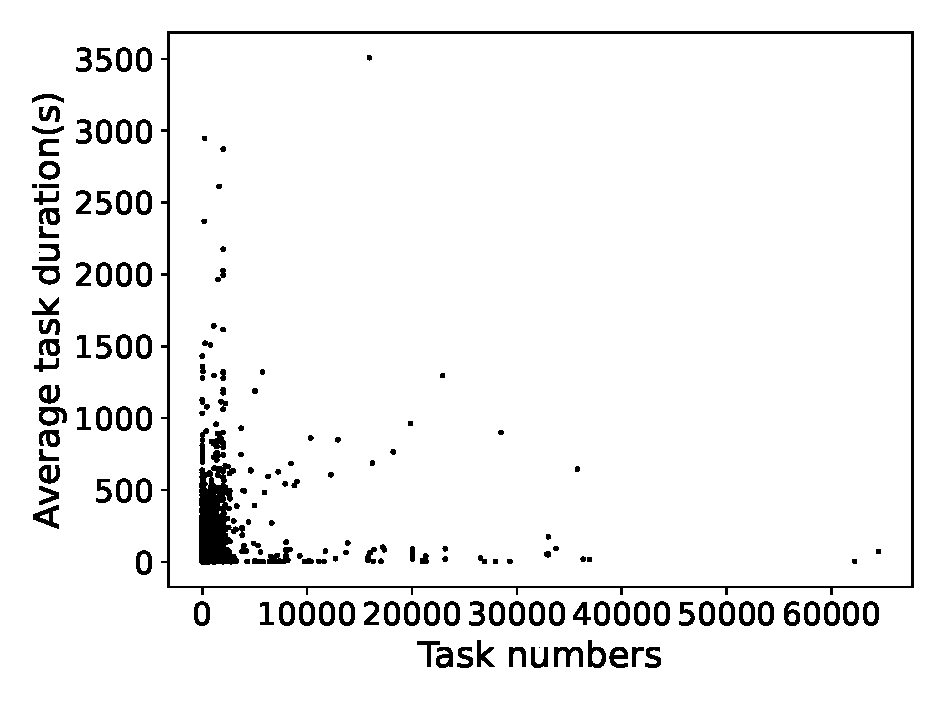
\includegraphics[width=0.48\linewidth]{Image/JobDistribution_Ali2017test2D.eps}%
    }
    \hfil
    \subfloat[Google Trace]
    {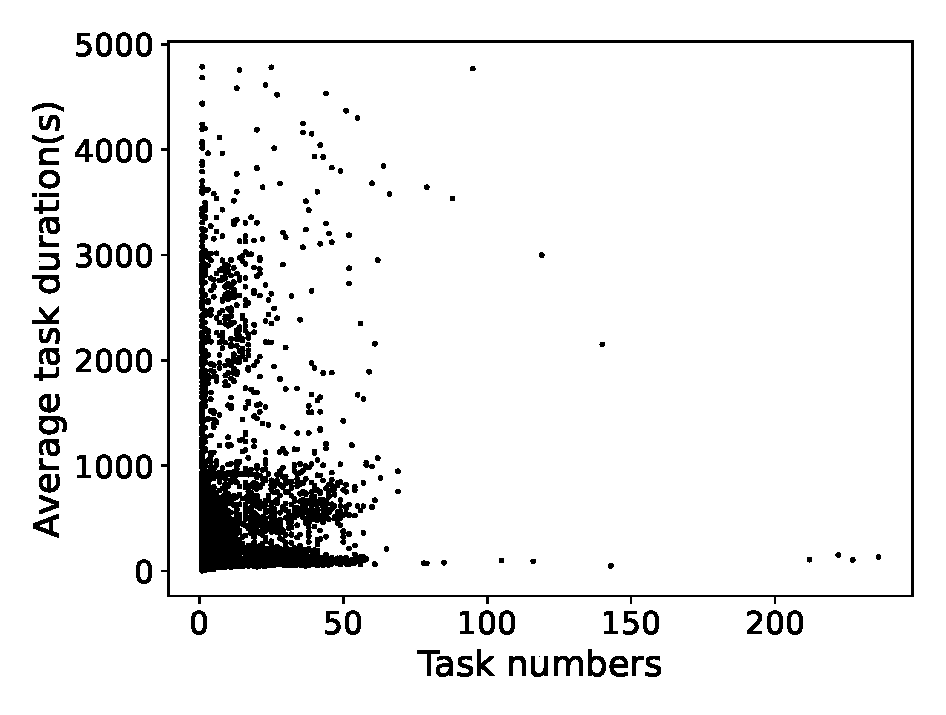
\includegraphics[width=0.48\linewidth]{Image/JobDistribution_Gg2019_112D.eps}%
    }
    \caption{Task characteristics of two datasets}
    \label{fig3:distribution}
\end{figure}

\begin{table}[tb]
\caption{Dataset characteristics}
    \centering
    \begin{tabular}{c c c}
     \toprule
     Dataset & Average task duration & Average task count per job \\
     \midrule
     Alibaba & $155.68$ seconds & $273.5$ tasks \\ 
     
     Google  & $512.25$ seconds & $4.5$ tasks\\ 
     \bottomrule
    \end{tabular}
    \label{tab3:data_characteristics}
\end{table}

\subsection{Datasets}
We use job traces from Alibaba \cite{Ali2017} and Google \cite{Gg2019}. The Alibaba trace contains information on approximately 16 million tasks collected from 1300 machines over a period of 12 hours in August 2017. The Google trace records events (e.g., a task is scheduled, completed or aborted) from Google's eight Borg cells over the month of May 2019. We pre-process the raw traces to extract key information, including the arrival time, task count and task durations of each job. From each trace, a continuous sequence of 15,000 jobs is randomly selected to serve as the dataset driving our simulations.

Figure \ref{fig3:distribution} and Table \ref{tab3:data_characteristics} illustrate the task characteristics of both datasets, including the task number and mean task duration of each job, and the average task duration and task count of all jobs. It can be seen that the jobs in the Alibaba dataset generally have larger numbers of tasks and shorter average task durations, whereas the jobs in the Google dataset tend to have longer average task durations and significantly fewer tasks.

\subsection{System Configuration}
We simulate a distributed system of $m$ sites, each with 32 computing slots. Each task is assumed to take up one computing slot to run and release it after completion. Due to the switching overhead consideration, we assume that there is no preemption during the execution of a task. For each job, the distribution of its tasks among the sites is generated by a Zipf distribution: the numbers of tasks placed on the sites are proportional to $1, \frac{1}{2^\alpha}, \frac{1}{3^\alpha}, ..., \frac{1}{m^\alpha}$, where $\alpha$ is a Zipf parameter. A higher $\alpha$ implies a more skewed distribution (a higher proportion of tasks are concentrated at one site), whereas $\alpha$ = $0.0$ indicates a uniform distribution. In the experiments, we test four Zipf distributions with $\alpha$ set to $0.0$, $0.5$, $1.0$ and $2.0$ to simulate different workload situations. We shuffle the order of the sites when deploying each job's task distribution, so that the overall workload distribution of all jobs is roughly balanced among sites. We scale the job arrival times to simulate different levels of overall system workloads. We experiment with different numbers of sites and different workload levels, and observe similar performance trends. We implement the algorithms and run the experiments on a server with AMD EPYC 7H12 2.6GHz processor and 1024GB memory.

\subsection{Resource Allocation Policies}
\label{resource_policy}
Besides Algorithms \ref{alg:basic} and \ref{alg:approx} (called DAMF and DAMF\_a for short), we also implement three baseline policies: IMF, AMF (both introduced in Section \ref{sec3:prelim}) and Dynamic Independent Max-min Fairness (DIMF). DIMF utilizes network resources on top of IMF: it first applies the IMF policy for resource allocation on each site, then transfers unsatisfied job demands to the sites with spare compute capacities to maximize the system utility (subject to the transfer limits), where jobs with lower aggregate allocations in the first step are assigned higher transmission priority in order to promote fairness. All the policies recompute the allocation matrix only when a new job arrives or an existing job completes all of its tasks on some site. We use CPLEX \cite{Cplex} as the program solver in the experiments. Since a task cannot be transferred fractionally, the transmission matrix $\Delta D$ derived to achieve the DAMF allocation may not be workable. To make DAMF applicable in practice, we enforce the elements of the transmission matrix $\Delta D$ in Algorithm \ref{alg:basic} to be integers, i.e., replacing the linear program with a mixed-integer program. This would incur extra but acceptable computation time. We shall demonstrate the computation times of DAMF and DAMF\_a later. Note that DAMF\_a does not need to apply a similar modification because the transmission matrix $\Delta D$ derived from its heuristic is always integral.

As introduced in Section \ref{sec:model_1}, transmission count limit $c$ is computed based on the average data partition size $S$, available bandwidth $B$ and time threshold $T$: $c = BT/S$. In the experiments, we set $T$ = 50 seconds (which is small compared to the average task duration shown in Table \ref{tab3:data_characteristics}), $S$ = 1GB and $B$ = 160Mbps or 480Mbps for all sites, thus $c = (160\; \text{or}\;480)*50/(1*1024*8) \approx 1\; \text{or}\; 3$. Under these settings, a task transmission generally takes $50/ (1\;\text{or}\;3)=50\;\text{or}\;16.67$ seconds to arrive at its destination. To emulate the bandwidth bottleneck being the connection between each site and the backbone network, task transmissions (potentially originating from different source sites) are received sequentially at each destination site. In recomputing the allocation and transmission matrices, the scheduler discards all pending transmissions (but retains the ongoing one) to release more bandwidth for the reallocation. For example, suppose $c=3$ for all sites and a recomputation is triggered $30$ seconds after the previous one. Suppose in the previous computation, it was decided that a site $S_j$ would receive $3$ tasks. In this case, the first task transmission would have arrived at site $S_j$ $16.67$ seconds after the previous computation, while the second task transmission is ongoing and the third one is pending. Then, in the recomputation, the third task transmission will be rescinded and the transmission count limit $c_j$ available for $S_j$ will be set to $2$.

\subsection{Performance Metrics}
In Sections \ref{sec:DAMF} and \ref{sec:property}, we have proved that DAMF achieves several important fairness properties. Our experiments aim to further evaluate DAMF and DAMF\_a's empirical performance from different perspectives. We study the following  performance metrics: the deviation of the instantaneous resource allocation from ideal DAMF, the standard deviation of the instantaneous resource allocation among jobs, the average Jain's Index of instantaneous resource allocation, and the average job response time. 

The deviation of the instantaneous resource allocation measures the instantaneous difference between the ideal DAMF allocation and the actual allocation of a policy. We continuously trace the number of computing slots actually occupied by each job throughout the simulation of different policies and compare it with the ideal DAMF allocation. More specifically, we first conduct the simulation using DAMF, and at each recomputation within simulation, we record the output transmission and allocation matrices as well as the resultant aggregate allocation vector with timestamp, which is taken as the ideal DAMF allocation. We also track the actual aggregate allocation of DAMF by updating the actual aggregate allocation vector with timestamp when a computing slot is allocated to a job (to run a task) or released by a job (when a task is completed). Note that available computing slots are assigned by the Hunger Degree mechanism and there is no preemption. Thus, the actual instantaneous allocations (resp. aggregate allocations) may differ from the allocation matrices (resp. aggregate allocation vectors) output by recomputations. Next, we perform simulations of other policies and record their actual allocations as well. Finally, we compute and trace the allocation deviation between an actual allocation and the ideal DAMF allocation over the simulated time span. Given two aggregate allocation vectors $\vec{A} = \langle a_1, a_2, ..., a_n \rangle.$ and $\vec{B} = \langle b_1, b_2, ..., b_n \rangle$, the allocation deviation is computed as $\sum_{i=1}^n |a_i - b_i|$. The allocations of completed jobs are treated as 0. A lower deviation indicates a closer instantaneous allocation to the ideal DAMF allocation. We plot the cumulative distribution of the deviation over the simulated time span. If the distribution curve is closer to the upper left corner, the allocation policy is considered to have better instantaneous fairness, because it has a lower deviation for a higher percentage of time. 

The standard deviation of the instantaneous resource allocation among jobs is computed from the records of the actual aggregate allocation vectors of jobs. We exclude jobs that have completed or not yet arrived from the computation of standard deviation. A lower standard deviation naturally indicates a more balanced resource allocation among jobs. We plot the cumulative distribution of the standard deviation over the simulated time span for comparison. Again, allocation policies whose distribution curves are closer to the upper left corner are considered superior in terms of instantaneous fairness. 

The Jain's Index is a quantitative measure used to assess the fairness or equity of resource allocation among $n$ competing users or entities. The range of Jain's Index is $[\frac{1}{n},1]$, and a higher index indicates a more balanced allocation. Suppose each user $i$ gets $x_i$ resources, then Jain's Index can be computed as follows:
\begin{equation*}
    f(x_1, x_2, \dots, x_n) = \frac{(\sum_{i=1}^nx_i)^2}{n*\sum_{i=1}^nx_i^2}.
\end{equation*}
We compute the Jain's Index from the records of the actual aggregate allocation vectors of jobs, and calculate the average Jain's Index over the simulated time span for comparison.

% \begin{figure*}[t]
% \centering
% \subfloat[Alibaba, workload = 40\%]
% {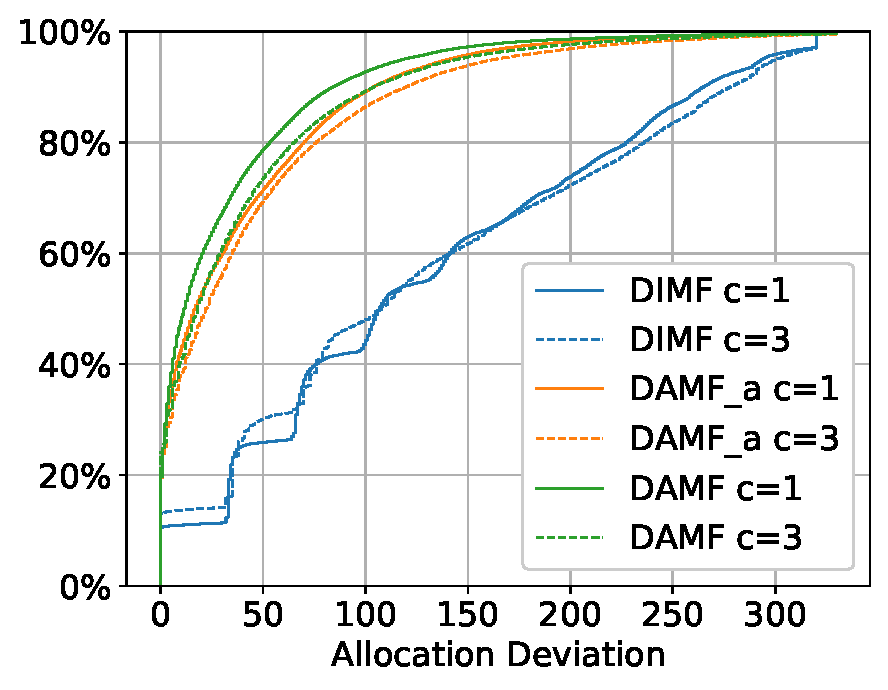
\includegraphics[width=0.24\textwidth]{Image/AD_Ali2017test_Alpha=2.0_40.eps}%
% %\label{fig_second_case}
% \label{Fg:AD_Ali_40}
% }
% \hfil
% \subfloat[Alibaba, workload = 60\%]
% %
% {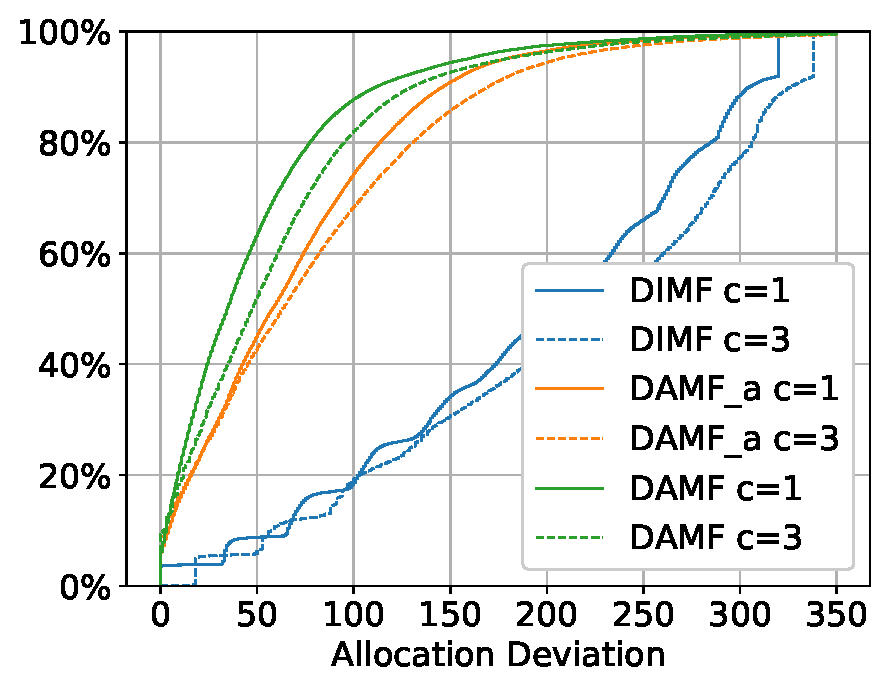
\includegraphics[width=0.24\textwidth]{Image/AD_Ali2017test_Alpha=2.0_60.eps}%
% \label{Fg:AD_Ali_60}
% }
% \hfil
% \subfloat[Google, workload = 40\%]
% %\label{Fg:eg3}
% {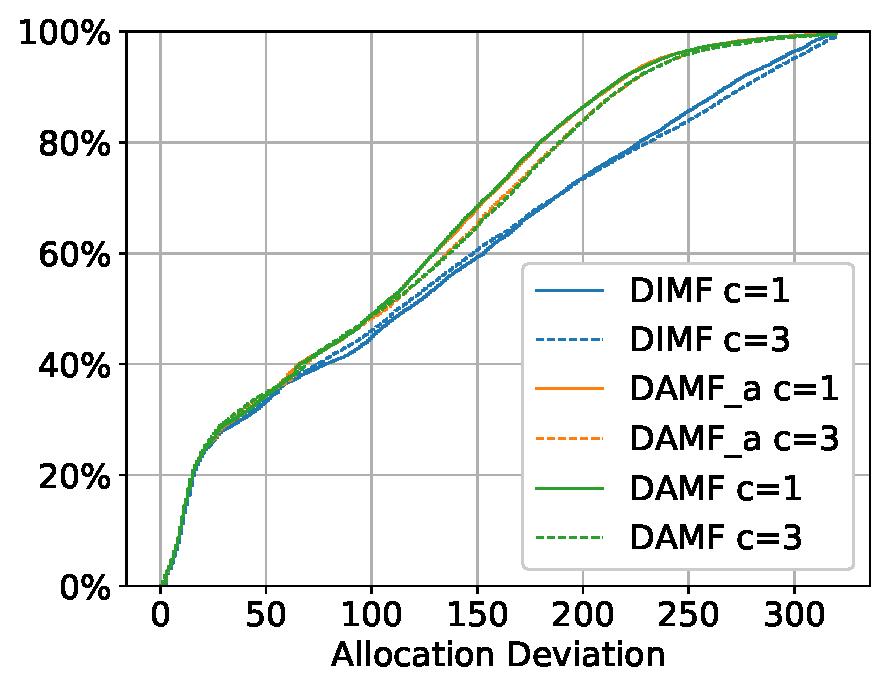
\includegraphics[width=0.24\textwidth]{Image/AD_Gg2019_11_Alpha=2.0_40.eps}%
% \label{Fg:AD_Gg_40}
% }
% \hfil
% \subfloat[Google, workload = 60\%]
% %\label{Fg:eg3}
% {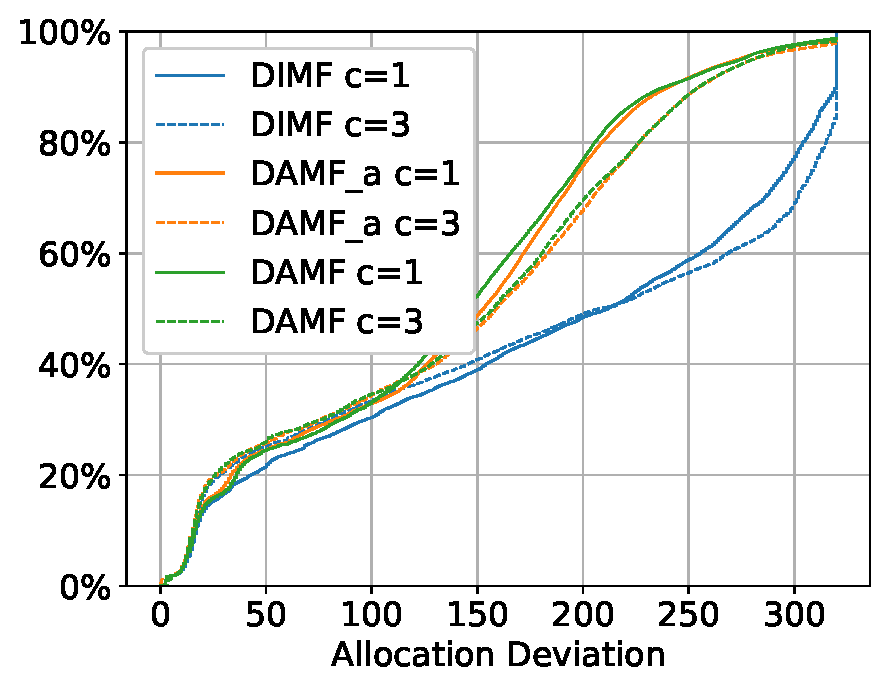
\includegraphics[width=0.24\textwidth]{Image/AD_Gg2019_11_Alpha=2.0_60.eps}%
% \label{Fg:AD_Gg_60}
% }
% \caption{Cumulative distribution of allocation deviation, Zipf parameter $\alpha = 2$}
% \label{fig:AD_instant}
% \end{figure*}

\begin{figure*}[t]
\centering
\subfloat[Alibaba, workload = 40\%]{
    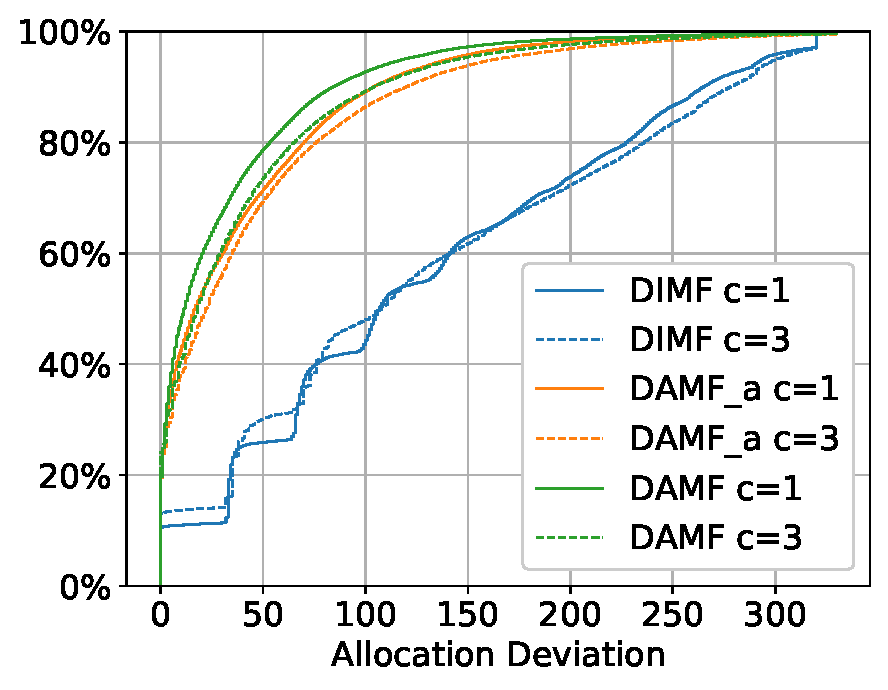
\includegraphics[width=0.47\textwidth]{Image/AD_Ali2017test_Alpha=2.0_40.eps}
    \label{Fg:AD_Ali_40}
}
\hfill
\subfloat[Alibaba, workload = 60\%]{
    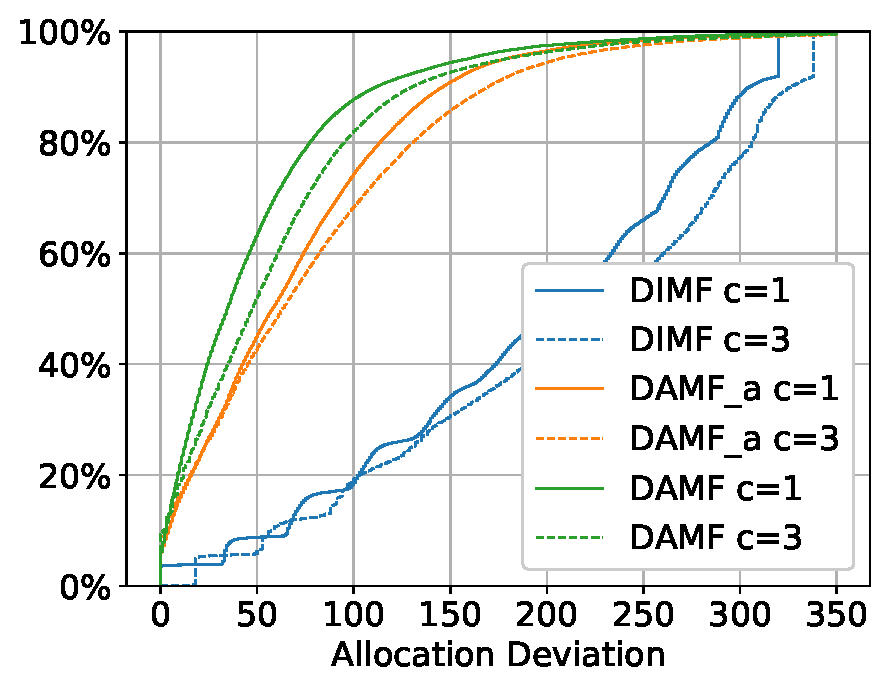
\includegraphics[width=0.47\textwidth]{Image/AD_Ali2017test_Alpha=2.0_60.eps}
    \label{Fg:AD_Ali_60}
}
\vspace{0.8em}
\subfloat[Google, workload = 40\%]{
    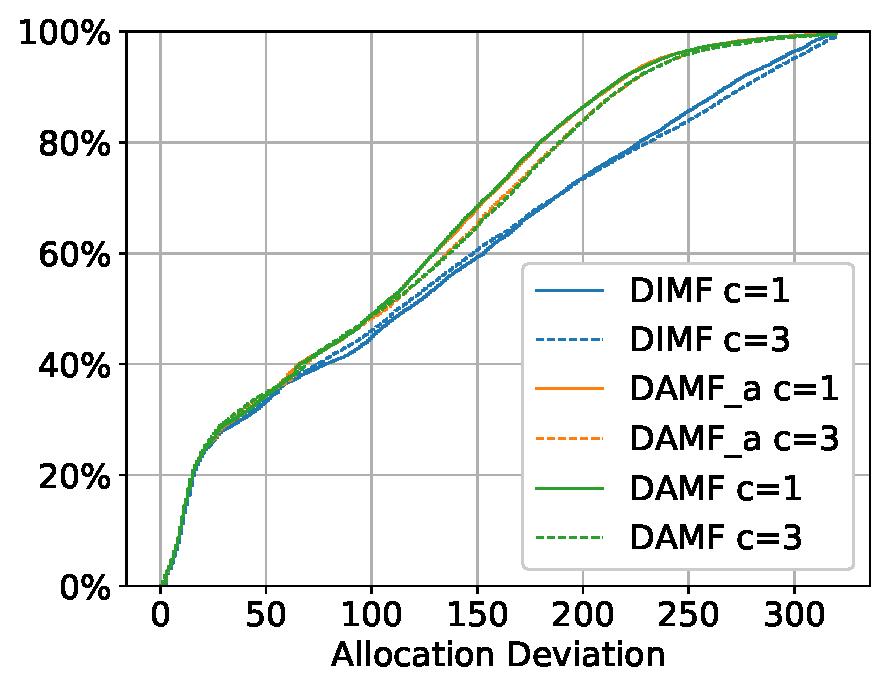
\includegraphics[width=0.47\textwidth]{Image/AD_Gg2019_11_Alpha=2.0_40.eps}
    \label{Fg:AD_Gg_40}
}
\hfill
\subfloat[Google, workload = 60\%]{
    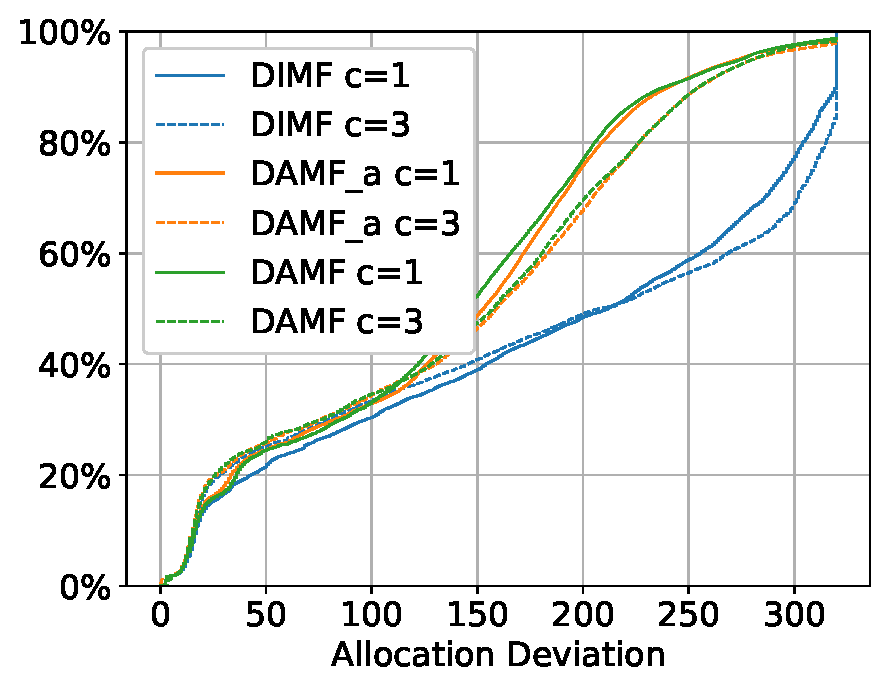
\includegraphics[width=0.47\textwidth]{Image/AD_Gg2019_11_Alpha=2.0_60.eps}
    \label{Fg:AD_Gg_60}
}
\caption{Cumulative distribution of allocation deviation, Zipf parameter $\alpha = 2$.}
\label{fig:AD_instant}
\end{figure*}


\begin{figure*}[t]
\centering
\subfloat[Alibaba, workload = 40\%]
{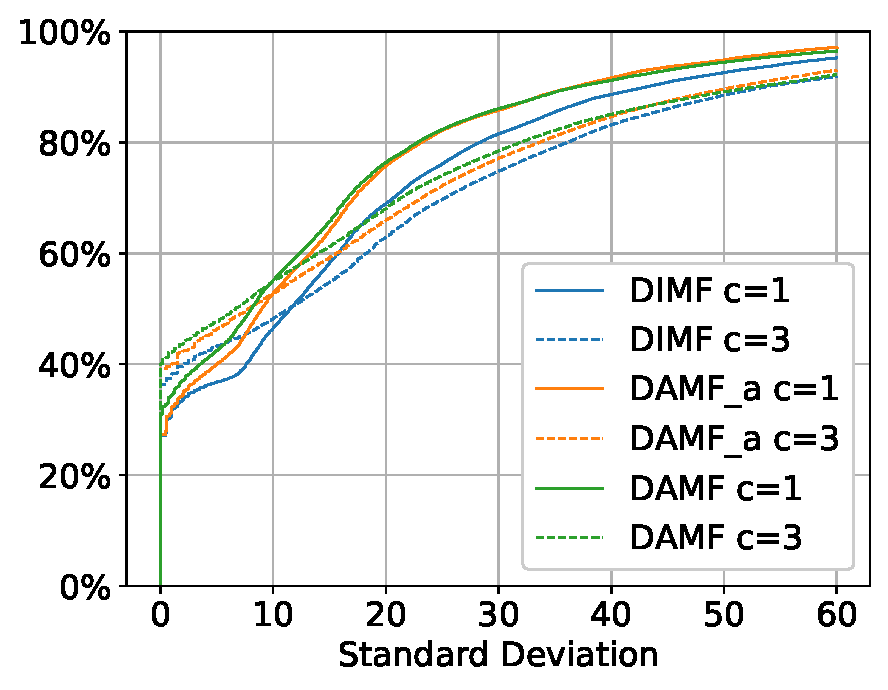
\includegraphics[width=0.48\textwidth]{Image/SD_Ali2017test_Alpha=2.0_40.eps}%
%\label{fig_second_case}
\label{Fg:SD_Ali_40}
}
\vspace{0.8em}
\subfloat[Alibaba, workload = 60\%]
%
{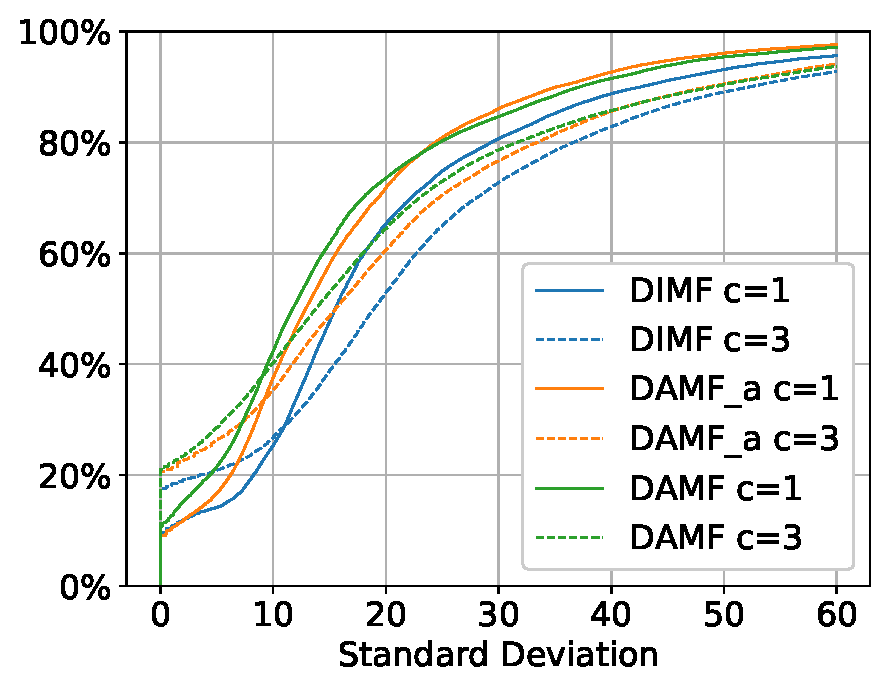
\includegraphics[width=0.48\textwidth]{Image/SD_Ali2017test_Alpha=2.0_60.eps}%
\label{Fg:SD_Ali_60}
}
\hfil
\subfloat[Google, workload = 40\%]
%\label{Fg:eg3}
{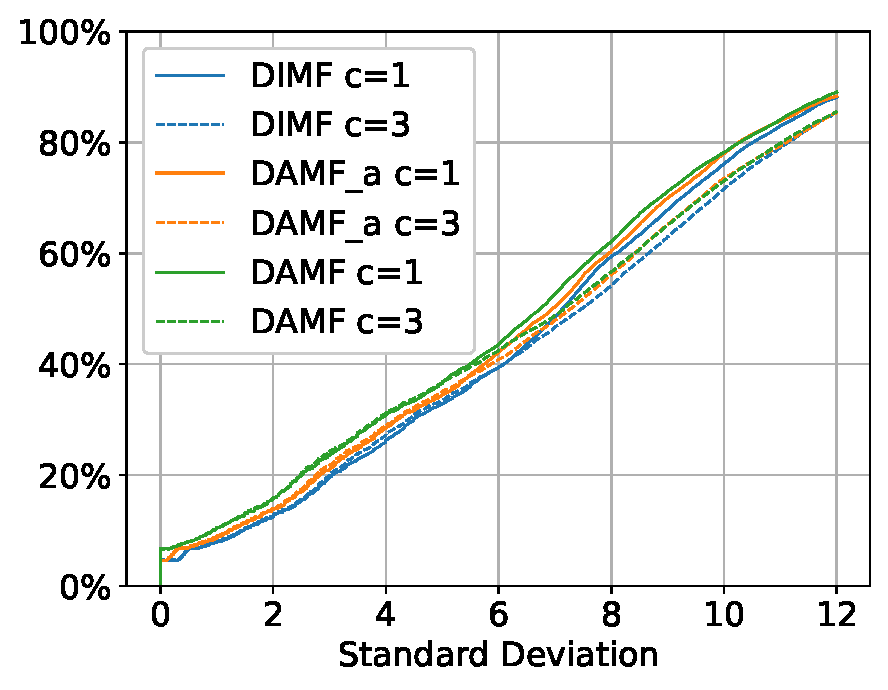
\includegraphics[width=0.48\textwidth]{Image/SD_Gg2019_11_Alpha=2.0_40.eps}%
\label{Fg:SD_Gg_40}
}
\hfil
\subfloat[Google, workload = 60\%]
%\label{Fg:eg3}
{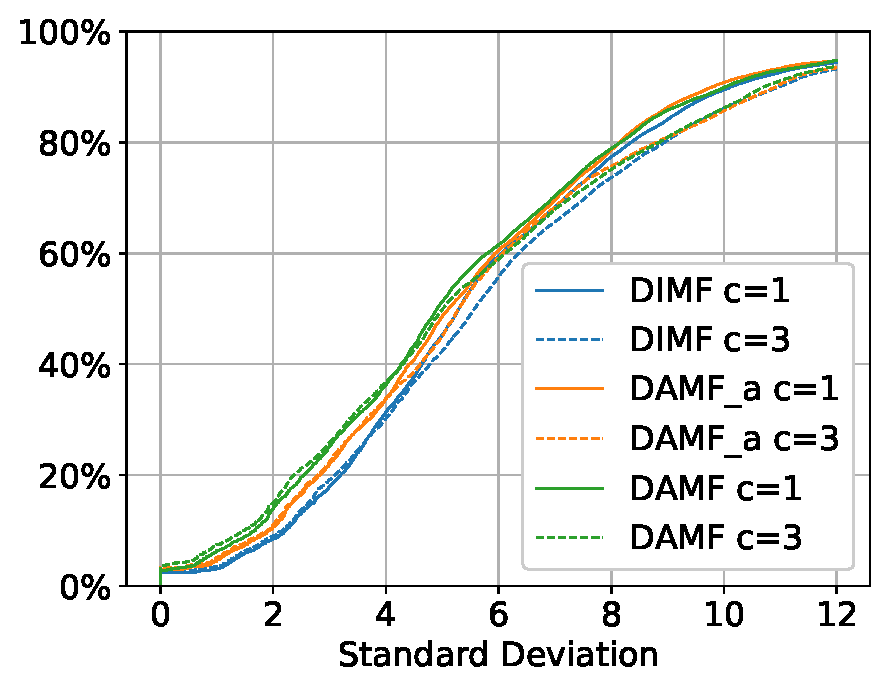
\includegraphics[width=0.48\textwidth]{Image/SD_Gg2019_11_Alpha=2.0_60.eps}%
\label{Fg:SD_Gg_60}
}
\caption{Cumulative distribution of standard deviation, Zipf parameter $\alpha = 2$}
\label{fig:SD_instant}
\end{figure*}

\begin{figure*}[htbp]
\centering
\subfloat[Alibaba, workload = 40\%]
{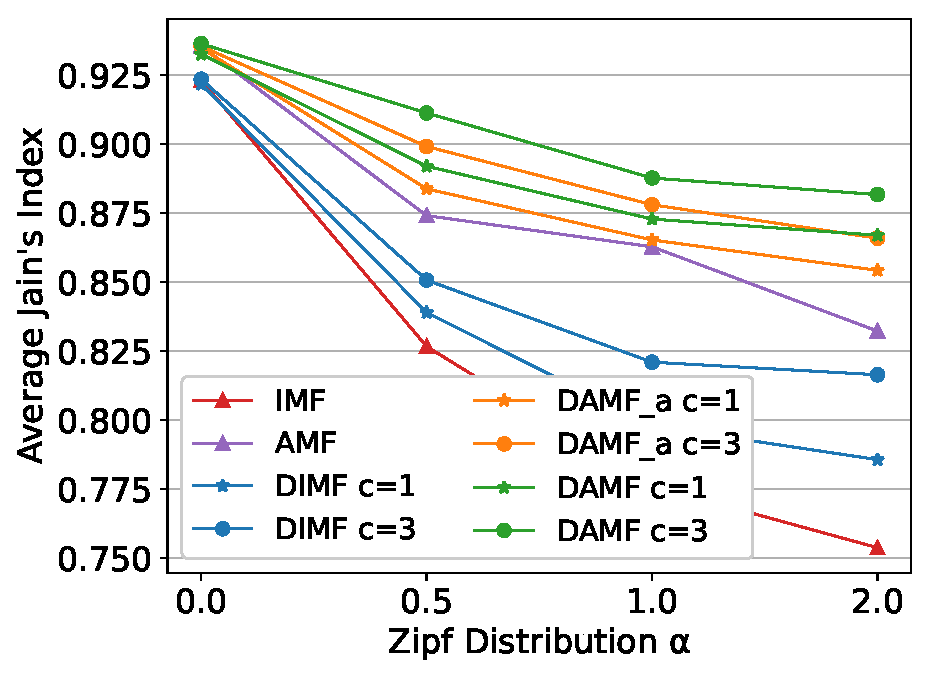
\includegraphics[width=0.48\textwidth]{Image/Jains_Ali2017test_40.eps}%
%\label{fig_second_case}
\label{Fg:Jains_Ali_40}
}
\hfil
\subfloat[Alibaba, workload = 60\%]
%
{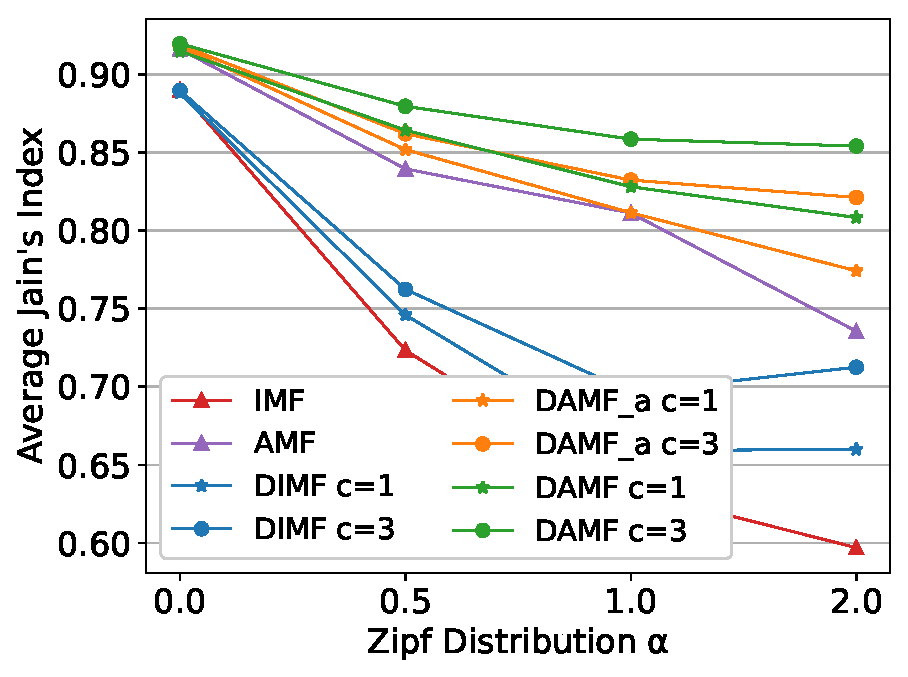
\includegraphics[width=0.48\textwidth]{Image/Jains_Ali2017test_60.eps}%
\label{Fg:Jains_Ali_60}
}
\vspace{0.8em}
\subfloat[Google, workload = 40\%]
%\label{Fg:eg3}
{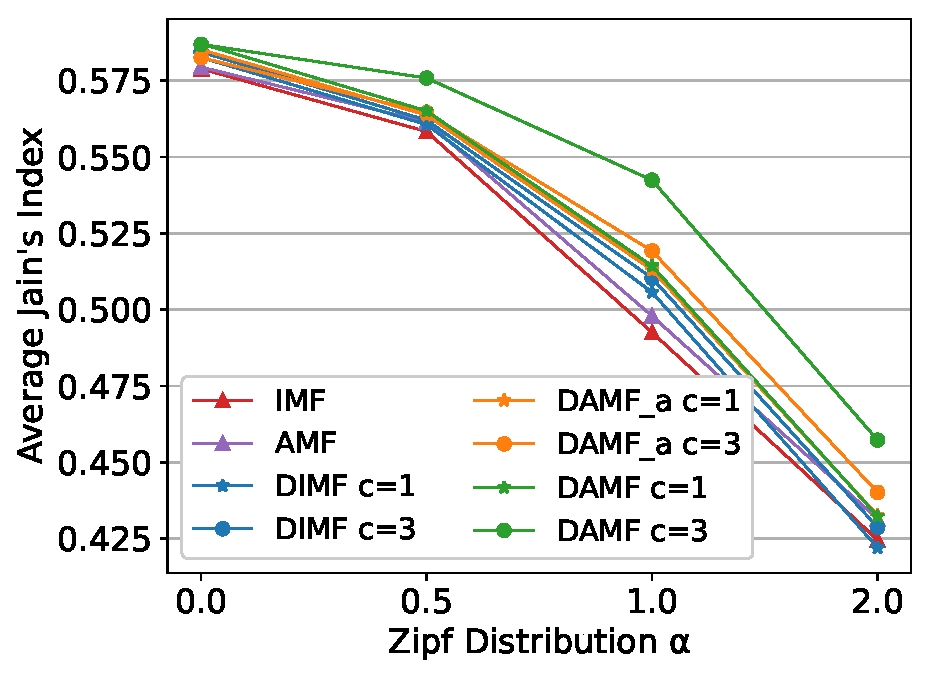
\includegraphics[width=0.48\textwidth]{Image/Jains_Gg2019_11_40.eps}%
\label{Fg:Jains_Gg_40}
}
\hfil
\subfloat[Google, workload = 60\%]
%\label{Fg:eg3}
{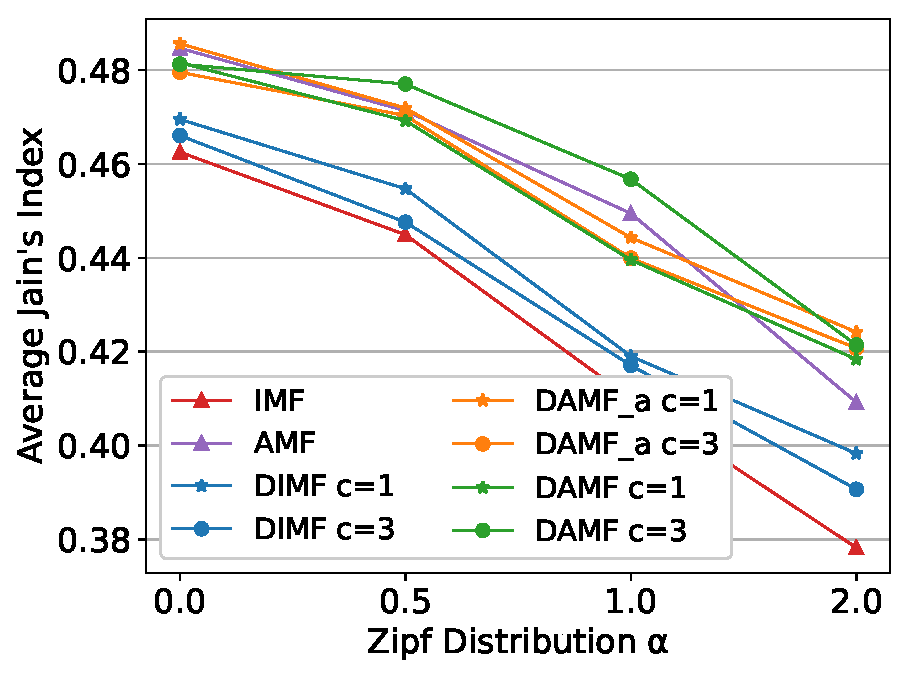
\includegraphics[width=0.48\textwidth]{Image/Jains_Gg2019_11_60.eps}%
\label{Fg:Jains_Gg_60}
}
\caption{Average Jain's Index}
\label{fig:Average Jain's Index}
\end{figure*}

\begin{figure*}[t]
\centering
\subfloat[Alibaba, workload = 40\%]
{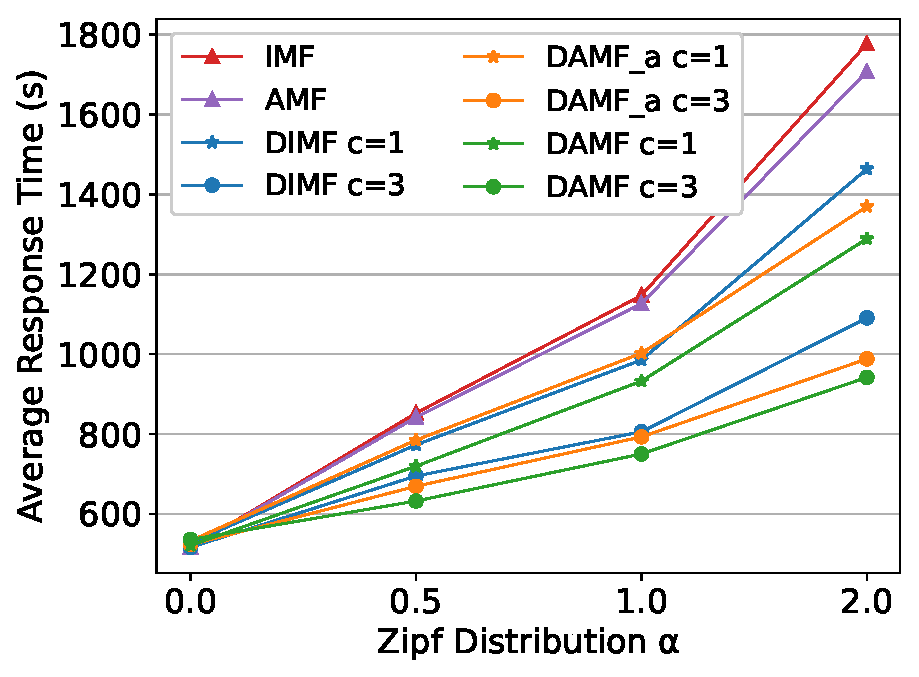
\includegraphics[width=0.48\textwidth]{Image/Workload_Ali2017test_40.eps}%
%\label{fig_second_case}
\label{Fg:JRT_Ali_40}
}
\hfil
\subfloat[Alibaba, workload = 60\%]
%
{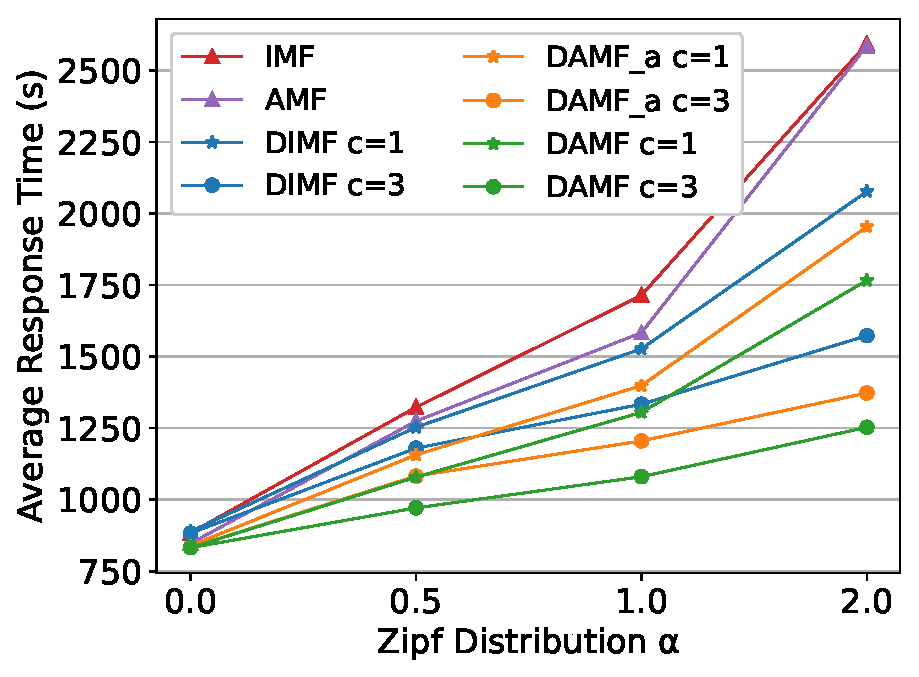
\includegraphics[width=0.48\textwidth]{Image/Workload_Ali2017test_60.eps}%
\label{Fg:JRT_Ali_60}
}
\vspace{0.8em}
\subfloat[Google, workload = 40\%]
%\label{Fg:eg3}
{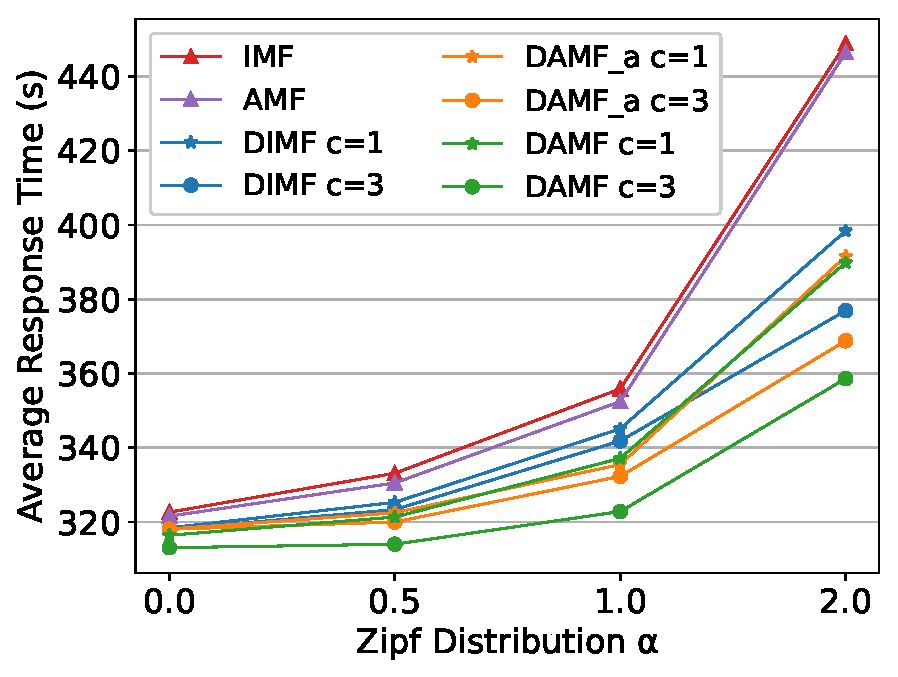
\includegraphics[width=0.48\textwidth]{Image/Workload_Gg2019_11_40.eps}%
\label{Fg:JRT_Gg_40}
}
\hfil
\subfloat[Google, workload = 60\%]
%\label{Fg:eg3}
{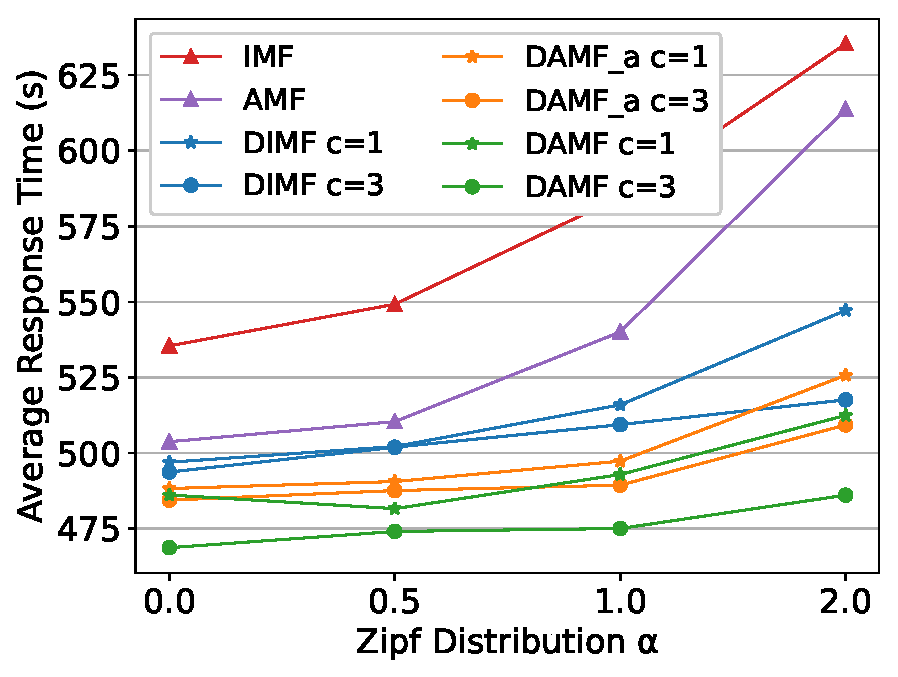
\includegraphics[width=0.48\textwidth]{Image/Workload_Gg2019_11_60.eps}%
\label{Fg:JRT_Gg_60}
}
\caption{Average job response time}
\label{fig:Average Response Time}
\end{figure*}

The response time of a job is the time duration from its arrival to its completion. We use the average job response time to evaluate the long-term impact of allocation policies. A lower average job response time suggests a higher system efficiency. 

\subsection{Experimental Results}

\begin{table}[t]
  \caption{Average computation time (s), Alibaba}
  \label{tab:computation_time_ali}
  \centering
    \begin{tabularx}{0.65\textwidth}{cccccc}
      \toprule
      & & \multicolumn{2}{c}{workload = 40\%} & \multicolumn{2}{c}{workload = 60\%} \\
      \midrule
      $c$ & $\alpha$ & DAMF & DAMF\_a & DAMF & DAMF\_a \\
      \midrule
      \multirow{4}{*}{1} 
      & 0.0 & $0.0747$ & $1.005*10^{-5}$ &  $0.1287$ & $1.402*10^{-5}$\\
      & 0.5 & $0.0792$ & $9.223*10^{-6}$&  $0.1661$ & $1.440*10^{-5}$\\
      & 1.0 & $0.0793$ & $9.409*10^{-6}$&  $0.1764$ & $1.453*10^{-5}$\\
      & 2.0 & $0.0841$ & $8.205*10^{-6}$&  $0.1709$ & $1.401*10^{-5}$\\
      \midrule
      \multirow{4}{*}{3} 
      & 0.0 & $0.0709$ & $8.749*10^{-6}$&  $0.1497$ & $1.690*10^{-5}$ \\
      & 0.5 & $0.0765$ & $8.395*10^{-6}$& $0.1571$ & $1.351*10^{-5}$ \\
      & 1.0 & $0.0761$ & $8.853*10^{-6}$& $0.1551$ & $1.424*10^{-5}$ \\
      & 2.0 & $0.0837$ & $1.051*10^{-5}$& $0.1733$ & $1.316*10^{-5}$ \\
      \bottomrule
    \end{tabularx}
\end{table}

\begin{table}[t]
  \caption{Average computation time (s), Google}
  \label{tab:computation_time_gg}
  \centering
    \begin{tabularx}{0.65\textwidth}{cccccc}
      \toprule
      & & \multicolumn{2}{c}{workload = 40\%} & \multicolumn{2}{c}{workload = 60\%}\\
      \midrule
      $c$ & $\alpha$ & DAMF & DAMF\_a & DAMF & DAMF\_a\\
      \midrule
      \multirow{4}{*}{1} 
      & 0.0 & $0.1029$ & $1.710*10^{-5}$ &$0.3783$ & $6.346*10^{-5}$ \\
      & 0.5 & $0.1247$ & $1.836*10^{-5}$ &$0.3771$ & $6.084*10^{-5}$ \\
      & 1.0 & $0.1298$ & $1.610*10^{-5}$&$0.3952$ & $5.071*10^{-5}$ \\
      & 2.0 & $0.1164$ & $1.686*10^{-5}$&$0.3708$ & $3.817*10^{-5}$ \\
      \midrule
      \multirow{4}{*}{3} 
      & 0.0 & $0.1180$ & $1.508*10^{-5}$&$0.4670$ & $7.205*10^{-5}$ \\
      & 0.5 & $0.1400$ & $1.583*10^{-5}$& $0.5175$ & $5.482*10^{-5}$ \\
      & 1.0 & $0.1489$ & $1.496*10^{-5}$& $0.5289$ & $5.178*10^{-5}$ \\
      & 2.0 &  $0.1796$ & $1.798*10^{-5}$ & $0.5465$ & $3.670*10^{-5}$ \\
      \bottomrule
    \end{tabularx}
\end{table}

Figure \ref{fig:AD_instant} shows the cumulative distribution of the allocation deviation from the ideal DAMF. Due to space limitations, we only present the results for the Zipf distribution of $\alpha = 2$. The results for other Zipf distributions show similar trends. Comparing DAMF and the baseline DIMF under the same transfer limit, it can be seen that DAMF's distribution curves are closer to the upper left corner, which indicates that DAMF achieves better instantaneous fairness than DIMF. In addition, the distribution curves of DAMF and DAMF\_a are rather close to each other under the same transfer limit, demonstrating that DAMF\_a is a close approximation of DAMF. We also record and compare the average computation time for recomputing allocation matrices during simulations. As shown in Table \ref{tab:computation_time_ali} and \ref{tab:computation_time_gg}, DAMF\_a reduces the average computation time by four orders of magnitude compared to DAMF (from the order of $10^{-1}$ seconds down to $10^{-5}$ seconds).

Comparing the results for the Alibaba and Google datasets under the same transfer limit, it can be seen that the Google dataset has much higher allocation deviations than the Alibaba dataset. This is mainly due to task durations: the Google dataset has much longer task durations than the Alibaba dataset as shown in Table \ref{tab3:data_characteristics}. Since there is no preemption, an updated allocation matrix after recomputation starts to take effect only after the computing slots are released (when the currently running tasks are completed) and reallocated to the intended jobs. Longer task durations make it slower for the actual allocation to converge to the allocation matrix computed.

Figure \ref{fig:SD_instant} shows the cumulative distribution of the standard deviation of the instantaneous resource allocation among jobs. Due to space limitations, we again only present the results for the Zipf distribution of $\alpha = 2$. Similar to the results in Figure \ref{fig:AD_instant}, it can be seen that DAMF’s distribution curves are closer to the upper left corner, which indicates that DAMF achieves more balanced instantaneous resource allocations than DIMF. Comparing DAMF and DAMF\_a under the same transfer limit, we can see that their distribution curves are quite close to each other, which again shows that DAMF\_a is a close approximation of DAMF. It can also be observed from Figure \ref{fig:SD_instant} that the standard deviation tends to increase with the transfer limit. This is because in DAMF, small-demand jobs are prioritized to have their demands fully satisfied at their original sites, while large-demand jobs are more likely to have unsatisfied demands and tend to exploit idle compute resources at other sites by leveraging network resources. Therefore, transmissions often help large-demand jobs to obtain more resources while keeping the resources allocated to small-demand jobs unchanged, which leads to the rise of the standard deviation of the instantaneous resource allocation with increasing transfer limit.

Figure \ref{fig:Average Jain's Index} shows the average Jain's Index. It can be seen that allocation policies that allow task transmissions (DAMF, DAMF\_a, DIMF) have higher Jain's Indexes compared with their counterparts which do not (AMF, IMF). More importantly, DAMF achieves the highest index while DAMF\_a is close to it, demonstrating that they effectively reduce the imbalance of resource allocation among jobs.

Figure \ref{fig:Average Response Time} shows the average job response time for different datasets, system workloads and Zipf distributions. It can be seen that policies utilizing network resources achieve lower average job response time, compared with IMF and AMF. The improvement typically increases with the transfer limit. Furthermore, since DAMF views the whole distributed system as a united resource pool and requires the aggregate allocation vector to be max-min fair among all possible transmissions and allocations, it outperforms DIMF and other allocation policies in most cases. The improvement is substantial even with only one bandwidth unit available, and it becomes more significant when the system workload is higher or the task distribution of jobs is more skewed among sites. In addition, DAMF\_a has similar performance of average job response time to DAMF, demonstrating that it closely approximates the original DAMF.

\subsection{Evaluation on Robustness and Scalability}

\begin{figure*}[t]
\centering
\subfloat[Alibaba, workload = 40\%]
{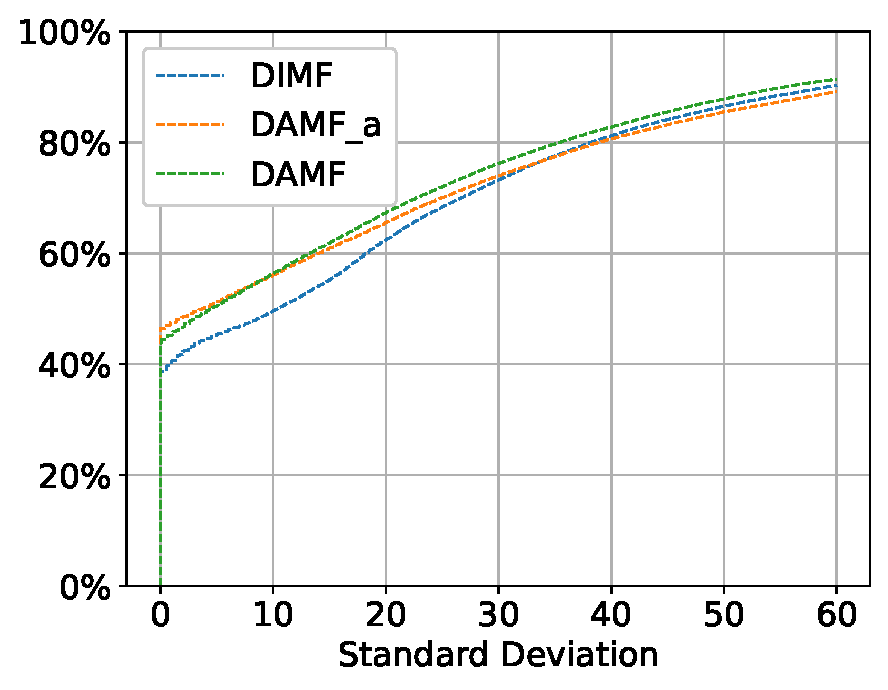
\includegraphics[width=0.48\textwidth]{Image/SD_Ali2017test_Alpha=2.0_40f.eps}
\label{Fg:SD_Ali_40f}
}
\hfil
\subfloat[Alibaba, workload = 60\%]
%
{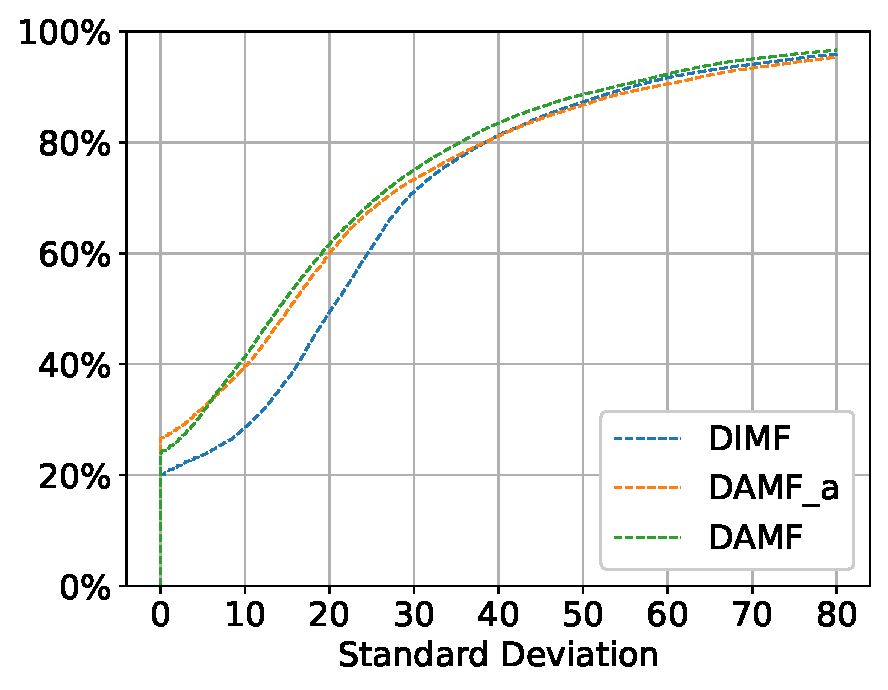
\includegraphics[width=0.48\textwidth]{Image/SD_Ali2017test_Alpha=2.0_60f.eps}%
\label{Fg:SD_Ali_60f}
}
\vspace{0.8em}
\subfloat[Google, workload = 40\%]
%
{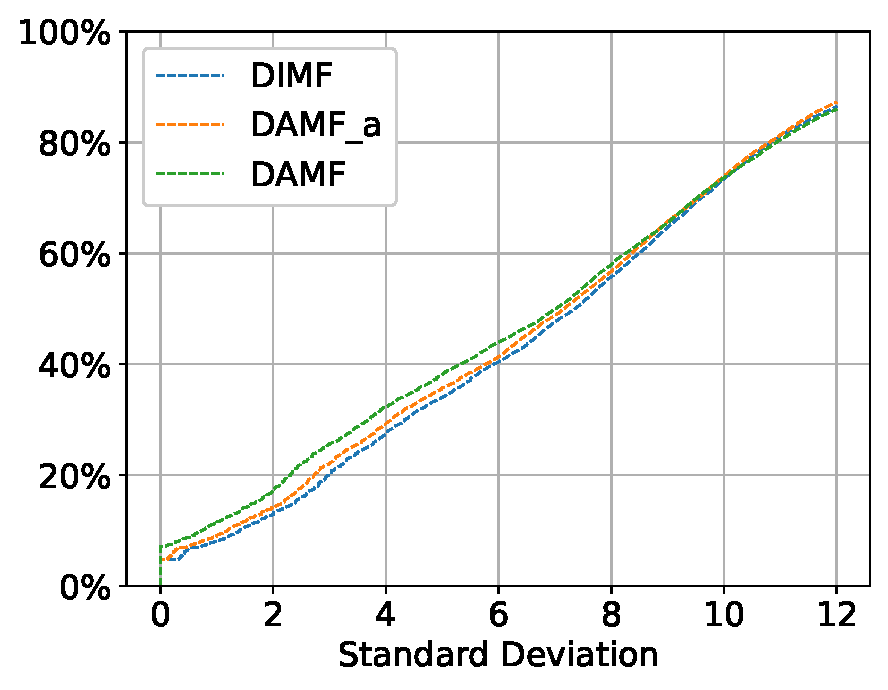
\includegraphics[width=0.48\textwidth]{Image/SD_Gg2019_11_Alpha=2.0_40f.eps}%
\label{Fg:SD_Gg_40f}
}
\hfil
\subfloat[Google, workload = 60\%]
%
{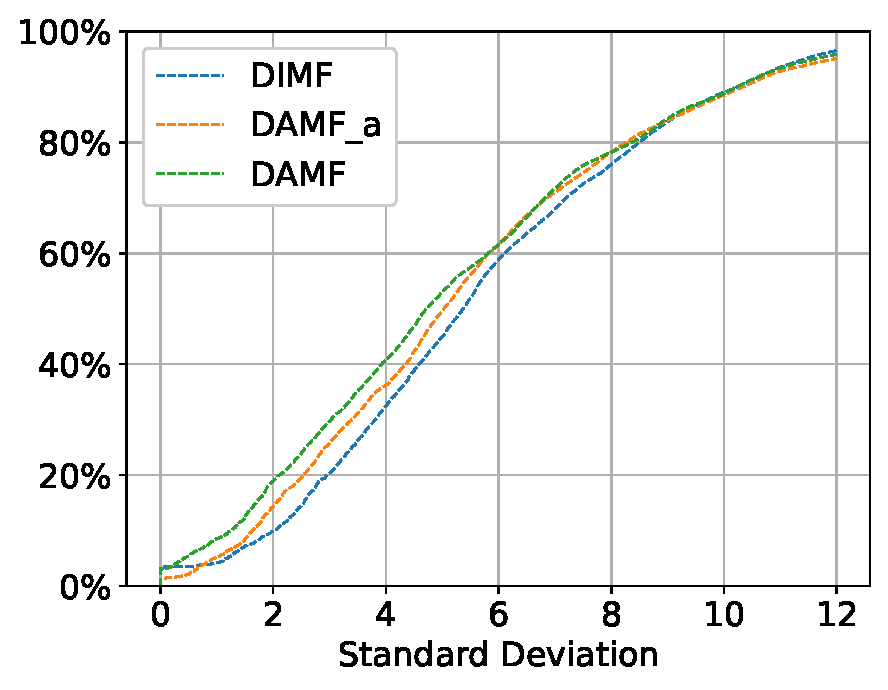
\includegraphics[width=0.48\textwidth]{Image/SD_Gg2019_11_Alpha=2.0_60f.eps}%
\label{Fg:SD_Gg_60f}
}
\caption{Cumulative distribution of standard deviation under fluctuating bandwidth, Zipf parameter $\alpha = 2$}
\label{fig:SD_f}
\end{figure*}

\begin{figure*}[t]
\centering
\subfloat[Alibaba, workload = 40\%]
{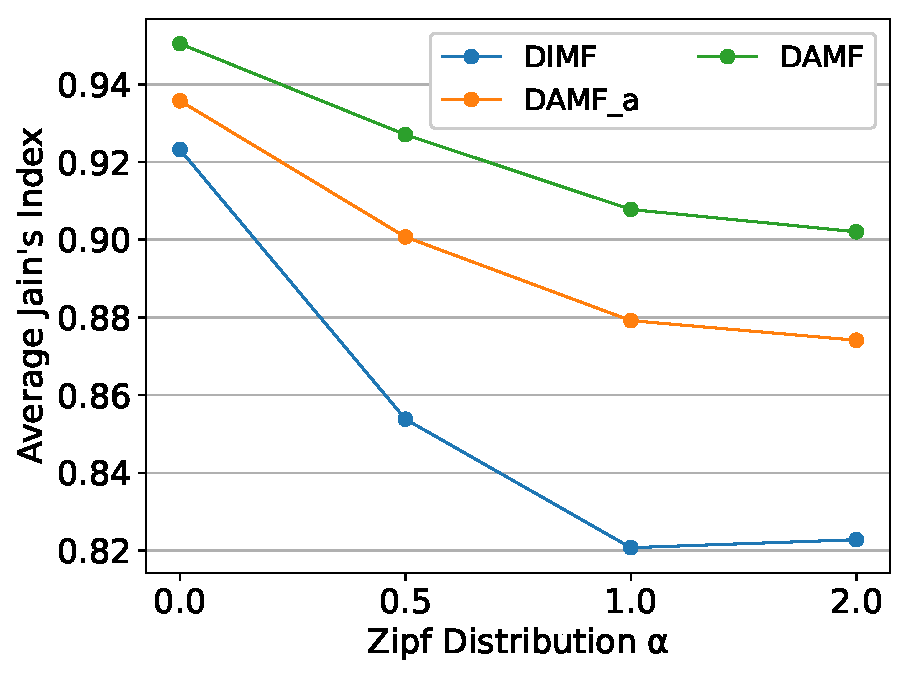
\includegraphics[width=0.48\textwidth]{Image/Jains_Ali2017test_40f.eps}%
\label{Fg:Jains_Ali_40f}
}
\hfil
\subfloat[Alibaba, workload = 60\%]
%
{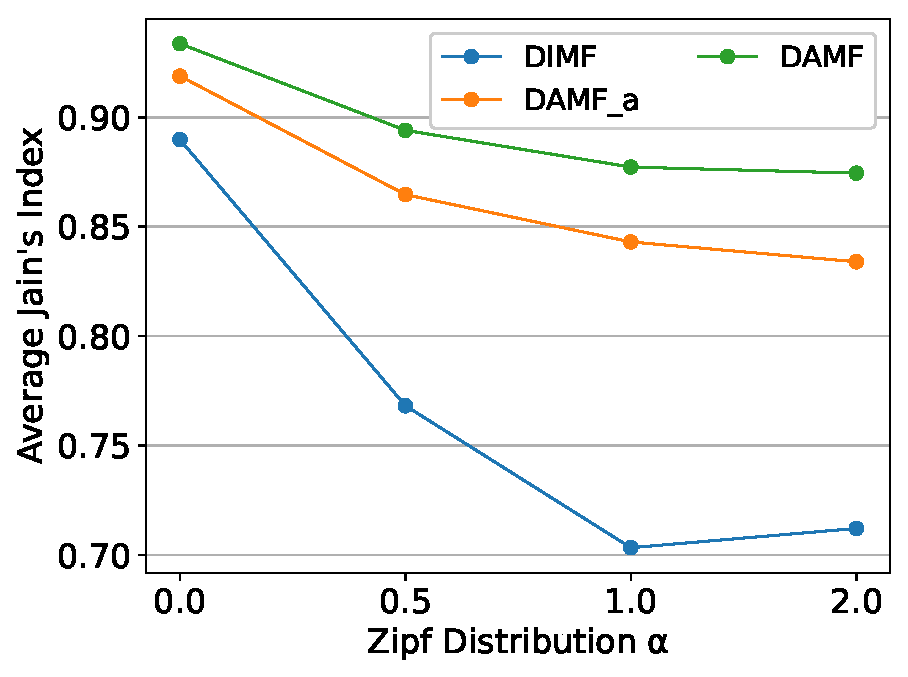
\includegraphics[width=0.48\textwidth]{Image/Jains_Ali2017test_60f.eps}%
\label{Fg:Jains_Ali_60f}
}
\vspace{0.8em}
\subfloat[Google, workload = 40\%]
%
{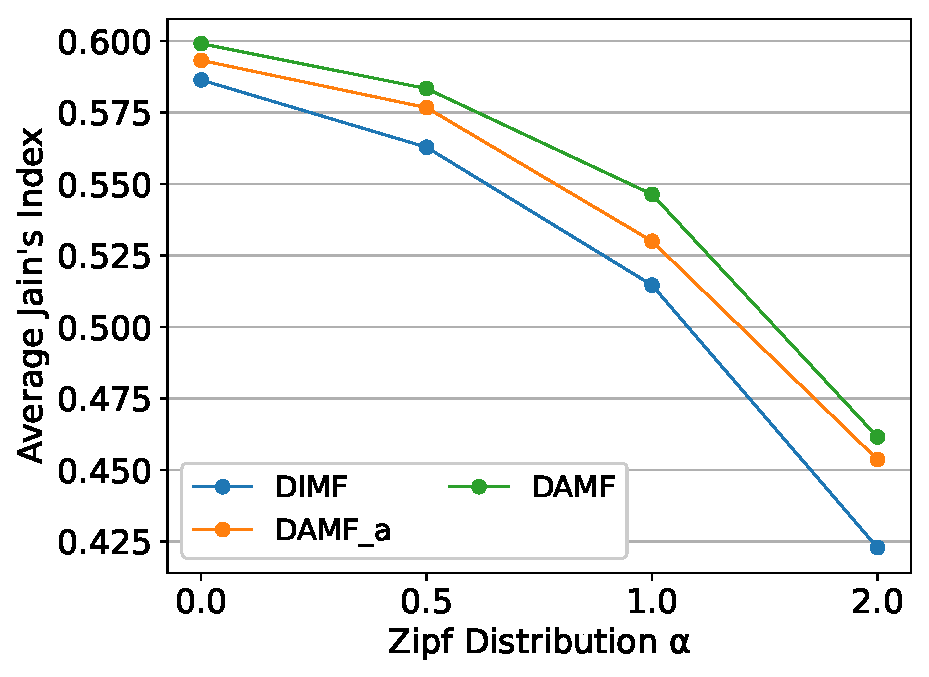
\includegraphics[width=0.48\textwidth]{Image/Jains_Gg2019_11_40f.eps}%
\label{Fg:Jains_Gg_40f}
}
\hfil
\subfloat[Google, workload = 60\%]
%
{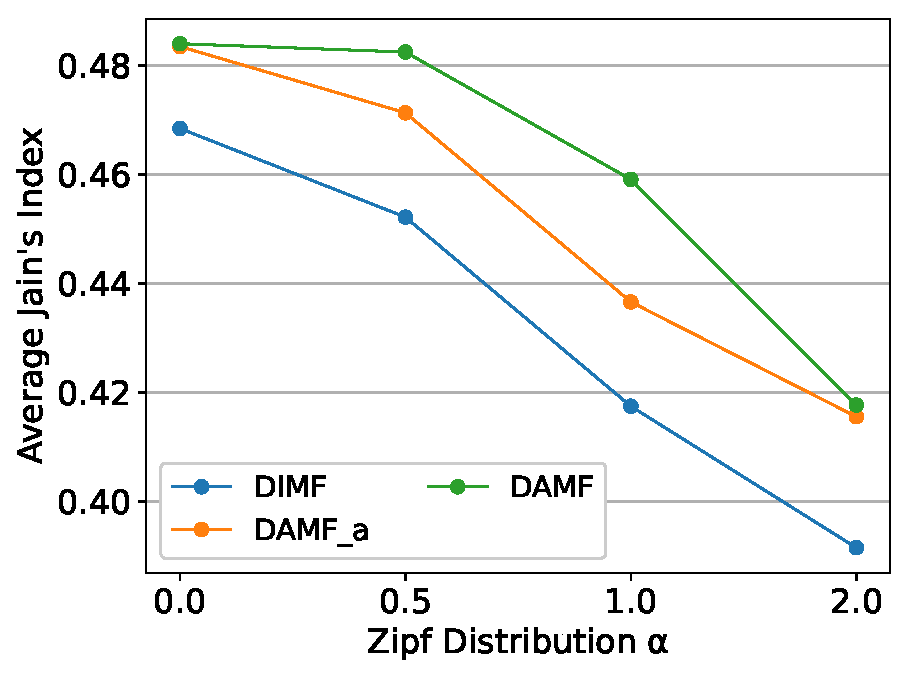
\includegraphics[width=0.48\textwidth]{Image/Jains_Gg2019_11_60f.eps}%
\label{Fg:Jains_Gg_60f}
}
\caption{Average Jain's Index under fluctuating bandwidth}
\label{fig:Average Jain's_f}
\end{figure*}

\begin{figure*}[t]
\centering
\subfloat[Alibaba, workload = 40\%]
{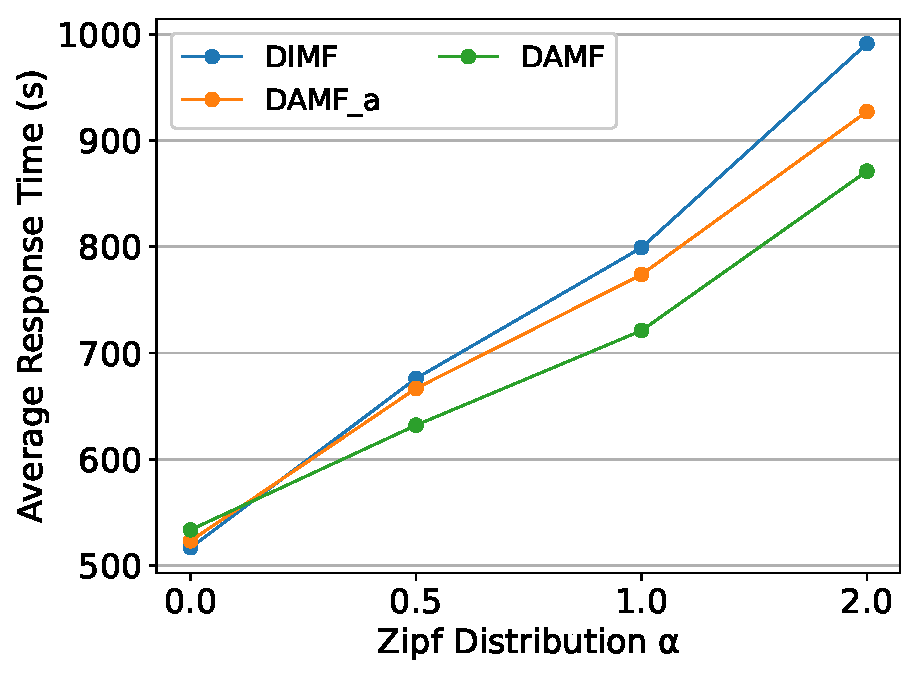
\includegraphics[width=0.48\textwidth]{Image/Workload_Ali2017test_40f.eps}%
\label{Fg:JRT_Ali_40f}
}
\hfil
\subfloat[Alibaba, workload = 60\%]
%
{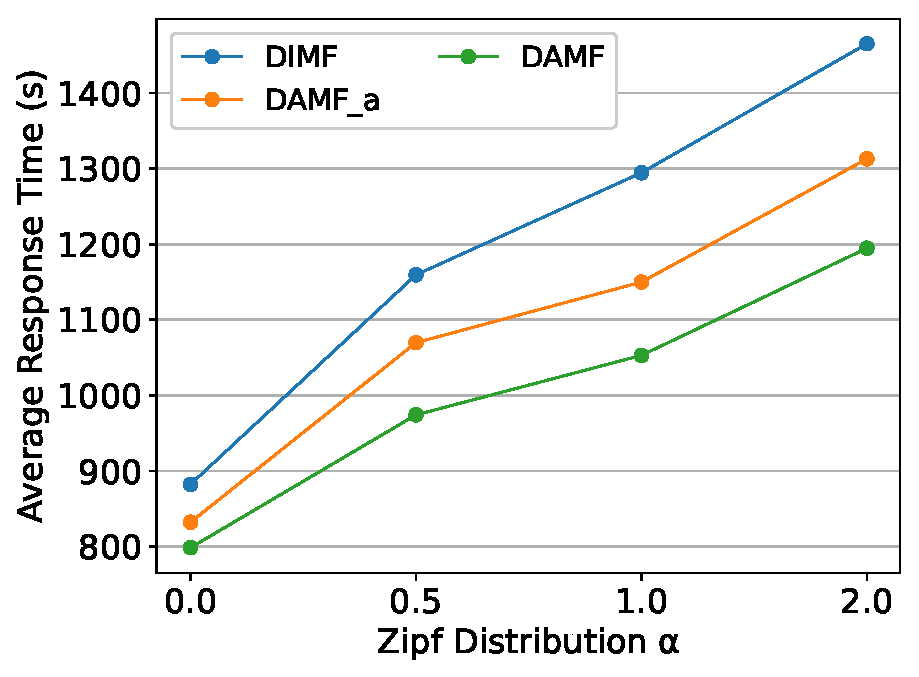
\includegraphics[width=0.48\textwidth]{Image/Workload_Ali2017test_60f.eps}%
\label{Fg:JRT_Ali_60f}
}
\vspace{0.8em}
\subfloat[Google, workload = 40\%]
%
{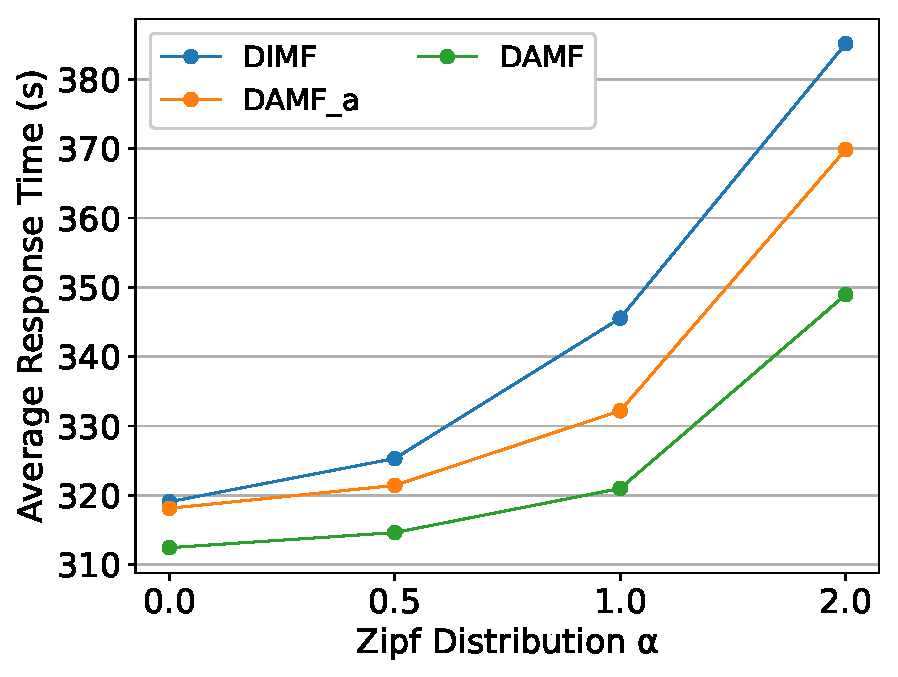
\includegraphics[width=0.48\textwidth]{Image/Workload_Gg2019_11_40f.eps}%
\label{Fg:JRT_Gg_40f}
}
\hfil
\subfloat[Google, workload = 60\%]
%
{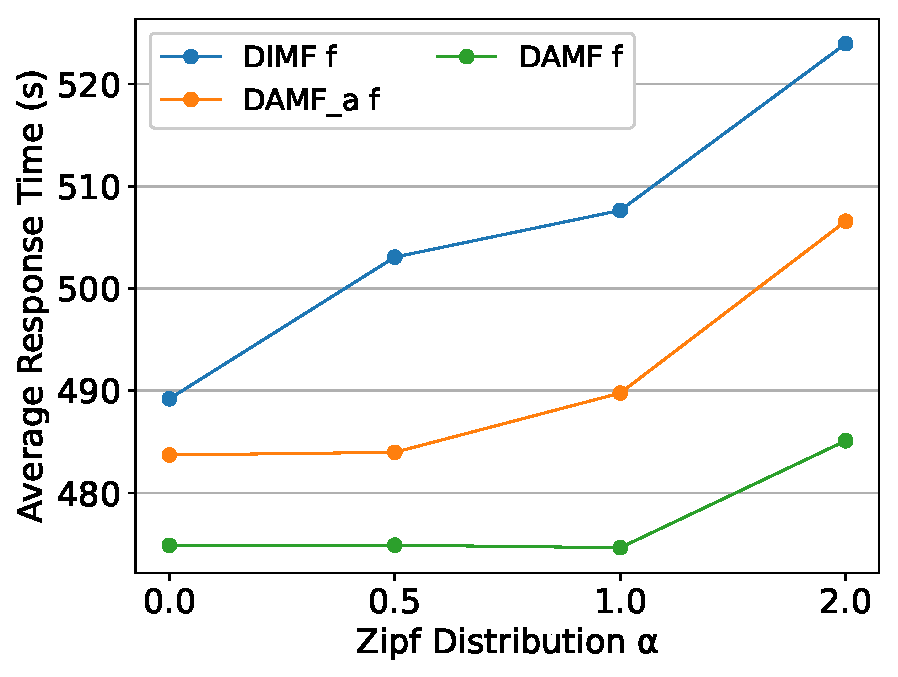
\includegraphics[width=0.48\textwidth]{Image/Workload_Gg2019_11_60f.eps}%
\label{Fg:JRT_Gg_60f}
}
\caption{Average job response time under fluctuating bandwidth}
\label{fig:Average Response Time_f}
\end{figure*}


We also conduct experiments to evaluate the allocation policies under fluctuating bandwidth conditions. Specifically, we initialize an integer sequence randomly generated from a uniform distribution between 1 and 5 to simulate the changes of the transfer count limit $c$ (which reflects the available bandwidth) over time. In the experiments, once the $i$-th job arrives, the value of $c$ for all sites is changed to the $i$-th element in the sequence for recomputation. For fair comparison, the same sequence is used for evaluating all allocation policies. As shown in Figures \ref{fig:SD_f}, \ref{fig:Average Jain's_f} and \ref{fig:Average Response Time_f}, the performance trends of different policies (that utilize network resources) remain similar to previous experiments. DAMF and DAMF\_a again significantly outperform the baseline policy DIMF.

In addition, we evaluate the scalability of DAMF\_a under larger numbers of sites $m$. We set $m=20$, $50$ and $100$ and conduct experiments for DAMF\_a and DIMF. Since the average task count per job of the Google dataset is low (4.5 tasks per job), it is not suitable for evaluation with a large number of sites. Thus, we test with the Alibaba dataset only. Due to space limitations, for performance metrics other than the average computation time, we present only the results for the Zipf distribution of $\alpha=1$ in Figures \ref{fig:SD_sites1}, \ref{fig:SD_sites2}, \ref{fig:Average_Response_Time_sites} and \ref{fig:Jains_sites} (those for other $\alpha$ values show similar trends). These results again demonstrate that DAMF\_a outperforms the baseline DIMF in terms of both resource allocation fairness and system utility. Table \ref{tab:computation_time_m} shows the average computation times for different site numbers and Zipf distributions. These results demonstrate that DAMF\_a maintains low computational overhead, thereby validating its potential for large-scale geo-distributed systems.

\begin{figure*}[t]
\centering
% 子图 1
\begin{subfigure}[b]{0.31\linewidth}
  \centering
  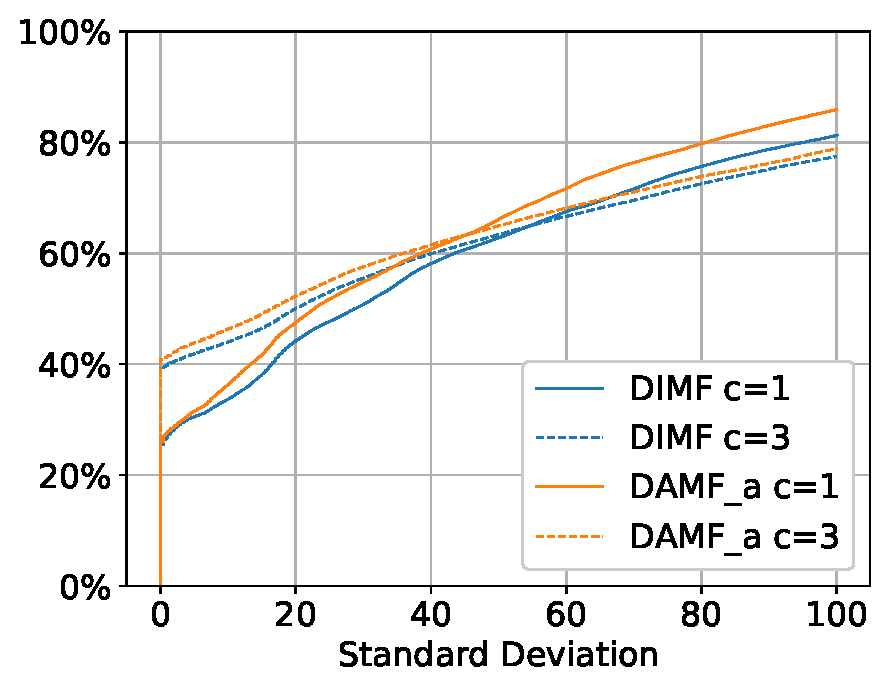
\includegraphics[width=\linewidth]{Image/SD_Ali2017test_Alpha=1.0_40_sites=20.eps}
  \caption{$m=20$}
  \label{Fg:SD_Ali_40_20m}
\end{subfigure}
\hfill % 用 \hfill 代替 \hfil，自动拉开完美的间距
% 子图 2
\begin{subfigure}[b]{0.31\linewidth}
  \centering
  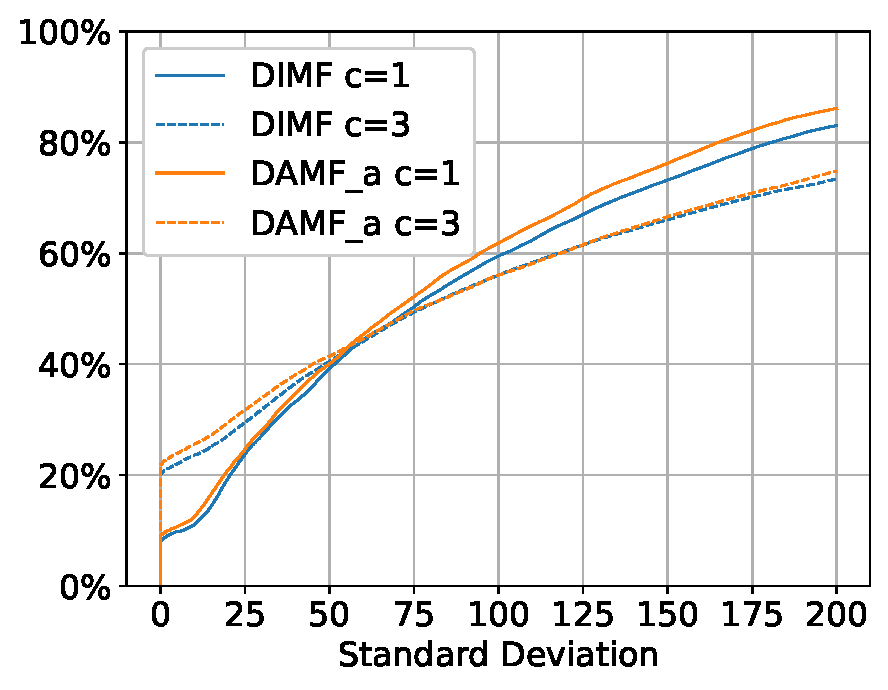
\includegraphics[width=\linewidth]{Image/SD_Ali2017test_Alpha=1.0_40_sites=50.eps}
  \caption{$m=50$}
  \label{Fg:SD_Ali_40_50m}
\end{subfigure}
\hfill
% 子图 3
\begin{subfigure}[b]{0.31\linewidth}
  \centering
  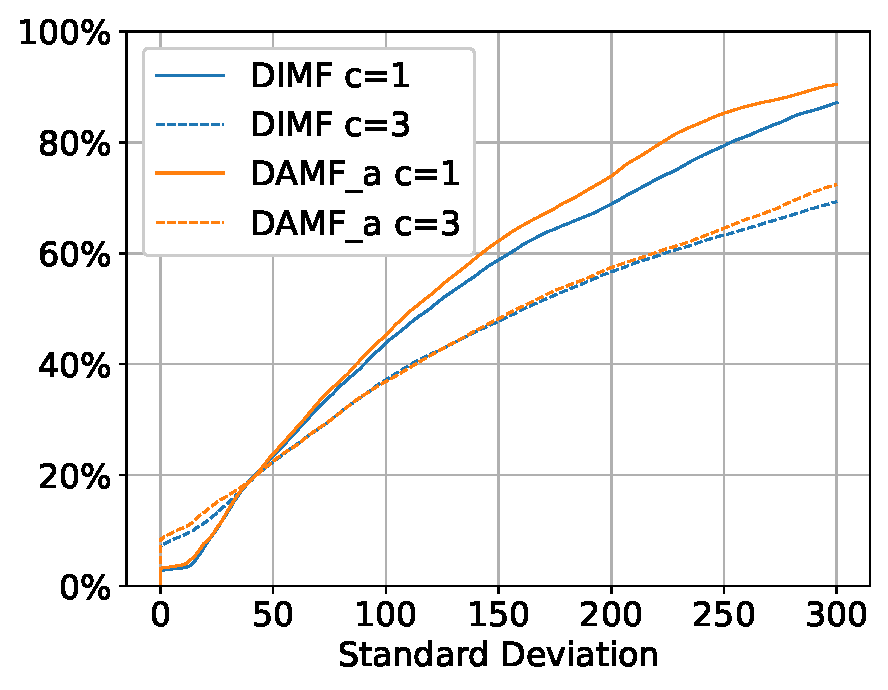
\includegraphics[width=\linewidth]{Image/SD_Ali2017test_Alpha=1.0_40_sites=100.eps}
  \caption{$m=100$}
  \label{Fg:SD_Ali_40_100m}
\end{subfigure}
\caption{Cumulative distribution of standard deviation, Alibaba, workload = 40\%, Zipf parameter $\alpha = 1$}
\label{fig:SD_sites1}
\end{figure*}

\begin{figure*}[t]
\centering
% 子图 1
\begin{subfigure}[b]{0.31\linewidth}
  \centering
  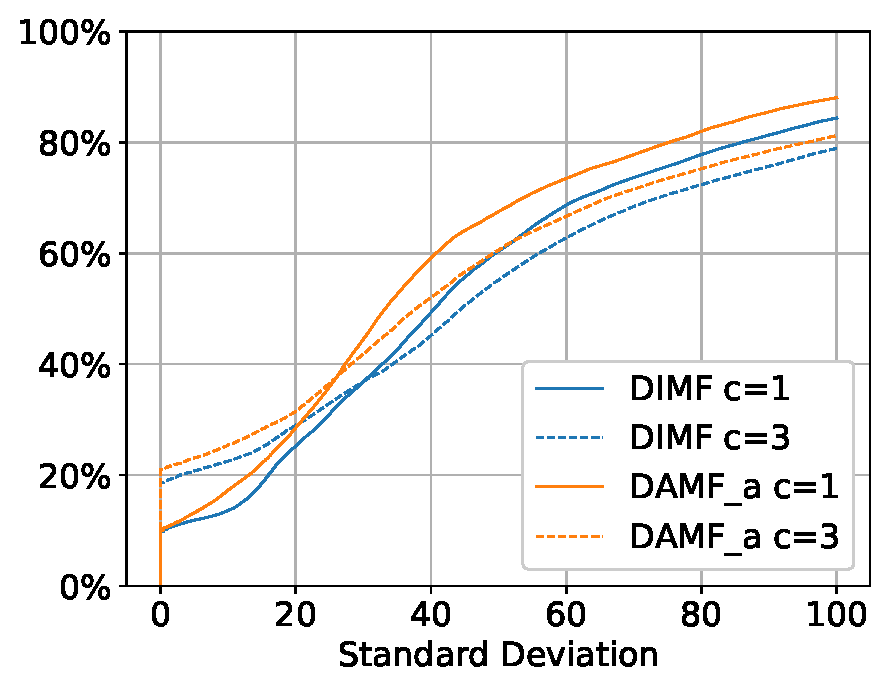
\includegraphics[width=\linewidth]{Image/SD_Ali2017test_Alpha=1.0_60_sites=20.eps}
  \caption{$m=20$}
  \label{Fg:SD_Ali_60_20m}
\end{subfigure}
\hfill % 用 \hfill 代替 \hfil，自动拉开完美的间距
% 子图 2
\begin{subfigure}[b]{0.31\linewidth}
  \centering
  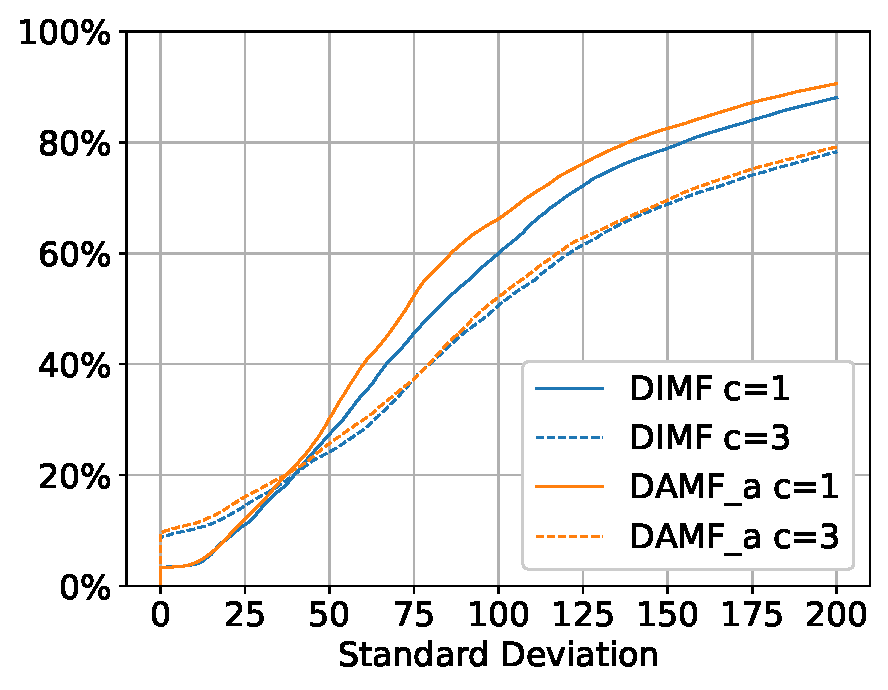
\includegraphics[width=\linewidth]{Image/SD_Ali2017test_Alpha=1.0_60_sites=50.eps}
  \caption{$m=50$}
  \label{Fg:SD_Ali_60_50m}
\end{subfigure}
\hfill
% 子图 3
\begin{subfigure}[b]{0.31\linewidth}
  \centering
  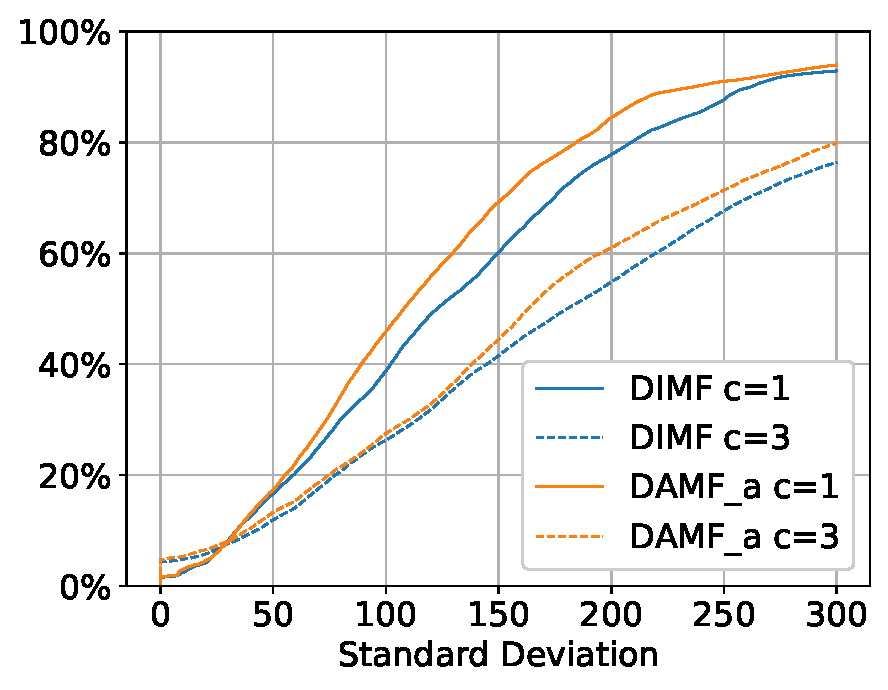
\includegraphics[width=\linewidth]{Image/SD_Ali2017test_Alpha=1.0_60_sites=100.eps}
  \caption{$m=100$}
  \label{Fg:SD_Ali_60_100m}
\end{subfigure}

\caption{Cumulative distribution of standard deviation, Alibaba, workload = 60\%, Zipf parameter $\alpha = 1$}
\label{fig:SD_sites2}
\end{figure*}

% \begin{figure}[t]
%   \centering
%   \begin{minipage}[b]{0.48\textwidth}
%     \centering
%     \subfloat[Alibaba, workload = 40\%]
%     {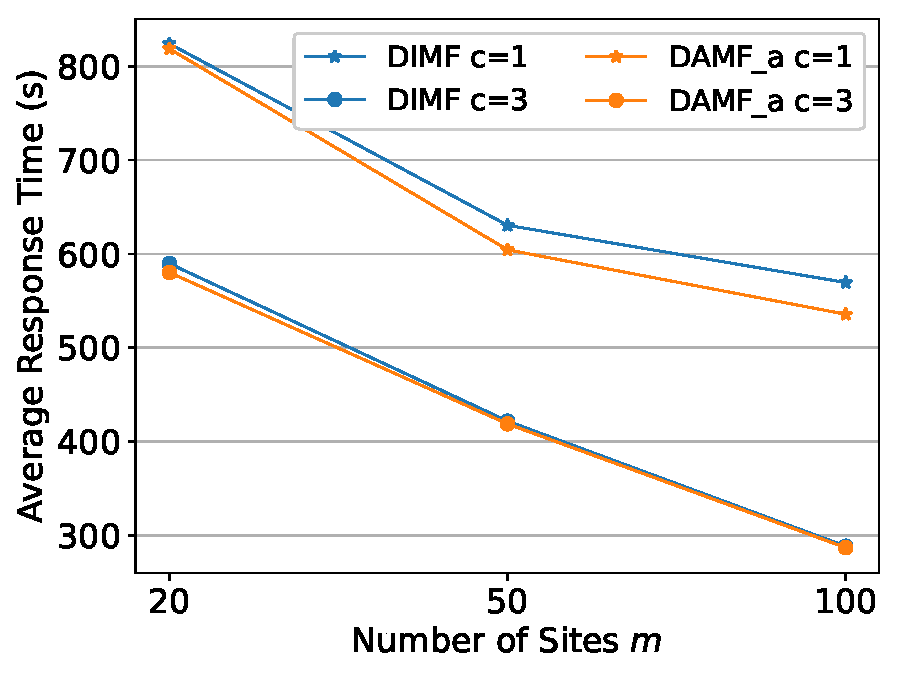
\includegraphics[width=0.48\linewidth]{Image/Workload_Ali2017test_40_site.eps}%
%     \label{Fg:JRT_Ali_40_m}
%     }
%     \hfil
%     \subfloat[Alibaba, workload = 60\%]
%     {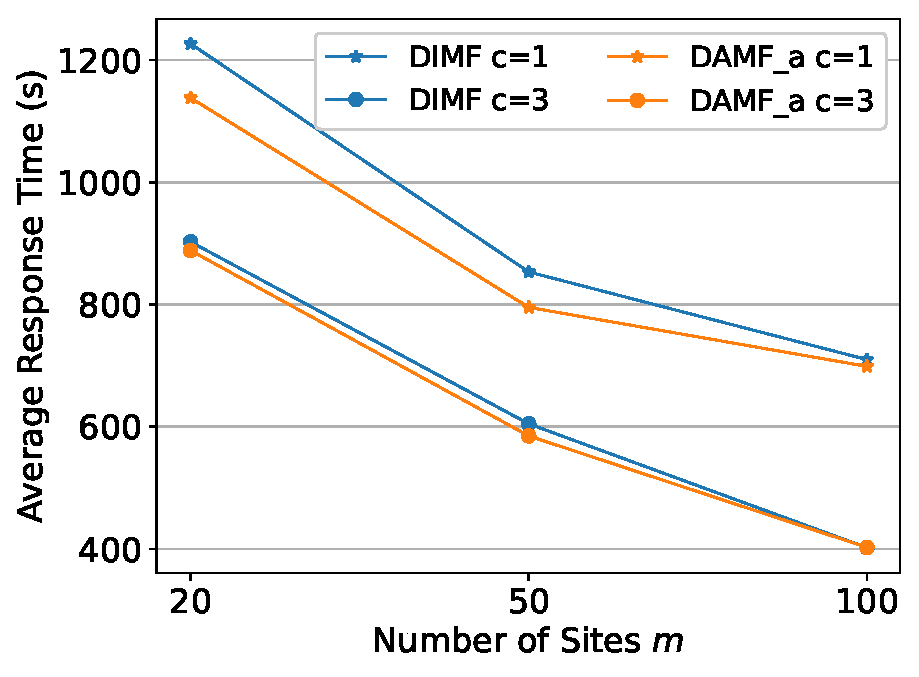
\includegraphics[width=0.48\linewidth]{Image/Workload_Ali2017test_60_site.eps}%
%     \label{Fg:JRT_Ali_60_m}
%     }
%     \caption{Average job response time, Zipf parameter $\alpha=1$}
%     \label{fig:Average Response Time_sites}
%   \end{minipage}
%   \hfill 
%   \begin{minipage}[b]{0.48\textwidth}
%     \centering
%     \subfloat[Alibaba, workload = 40\%]
%     {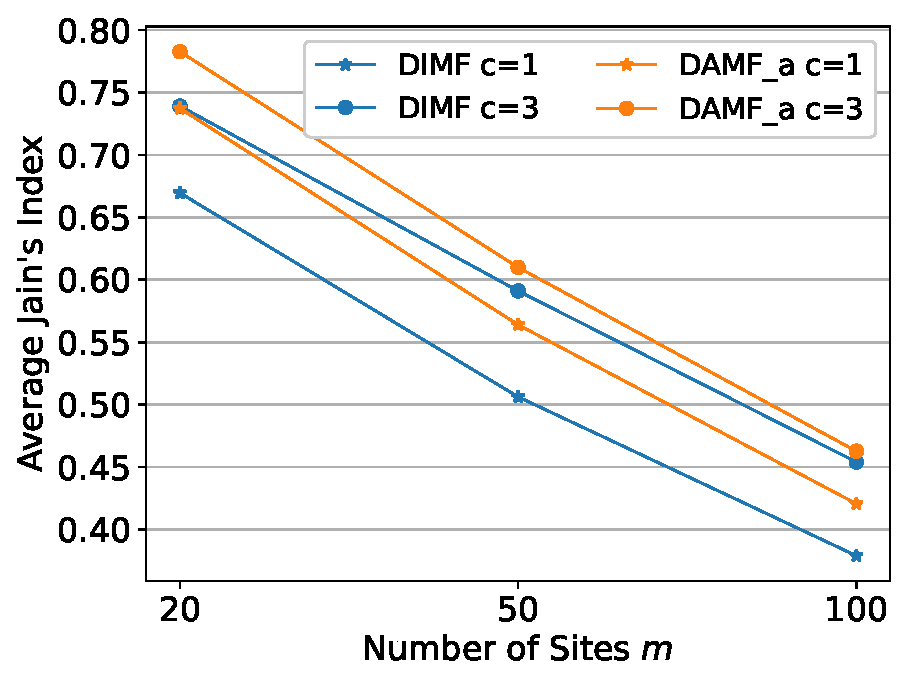
\includegraphics[width=0.48\linewidth]{Image/Jains_Ali2017test_40_site.eps}%
%     \label{Fg:Jains_Ali_40_m} % 
%     }
%     \hfil
%     \subfloat[Alibaba, workload = 60\%]
%     {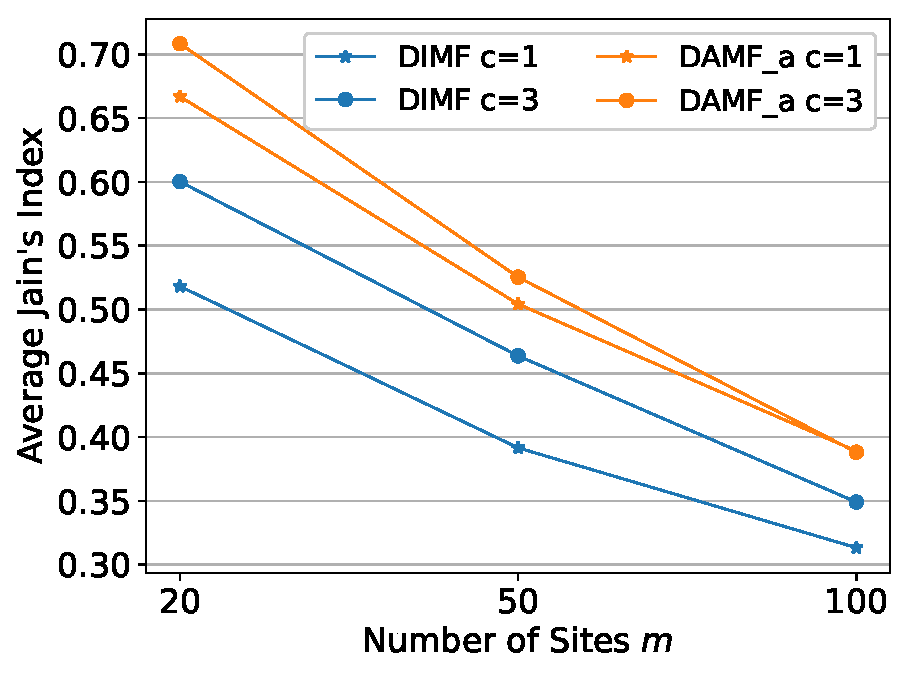
\includegraphics[width=0.48\linewidth]{Image/Jains_Ali2017test_60_site.eps}%
%     \label{Fg:Jains_Ali_60_m} % 
%     }
%     \caption{Average Jain's Index, Zipf parameter $\alpha=1$}
%     \label{fig:Jains_sites}
%   \end{minipage}
% \end{figure}

\begin{figure}[t]
    \centering
    \subfloat[Alibaba, workload = 40\%]
    {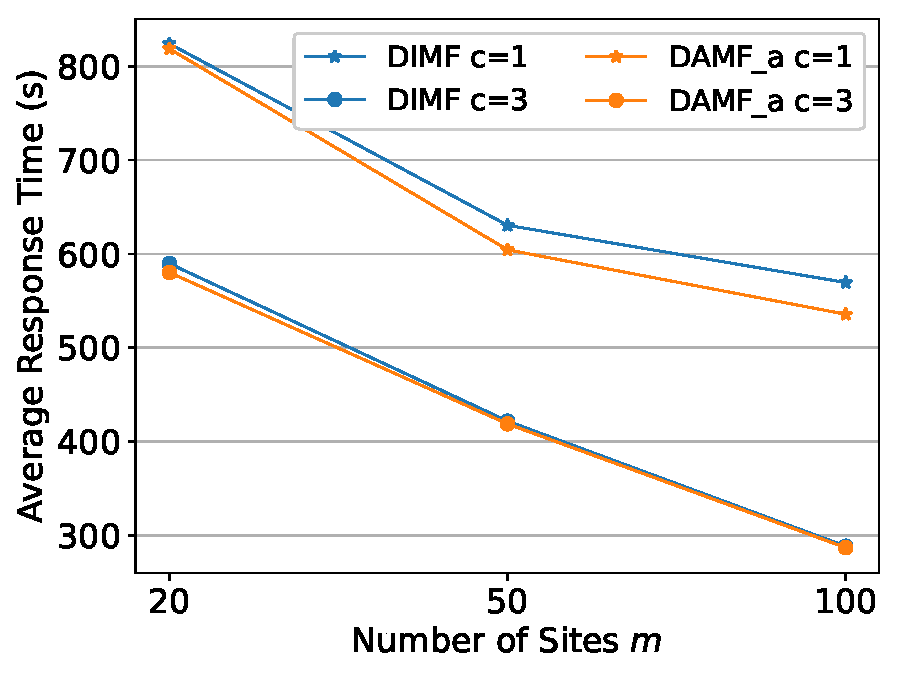
\includegraphics[width=0.48\linewidth]{Image/Workload_Ali2017test_40_site.eps}
    \label{Fg:JRT_Ali_40_m}}
    \hfill
    \subfloat[Alibaba, workload = 60\%]
    {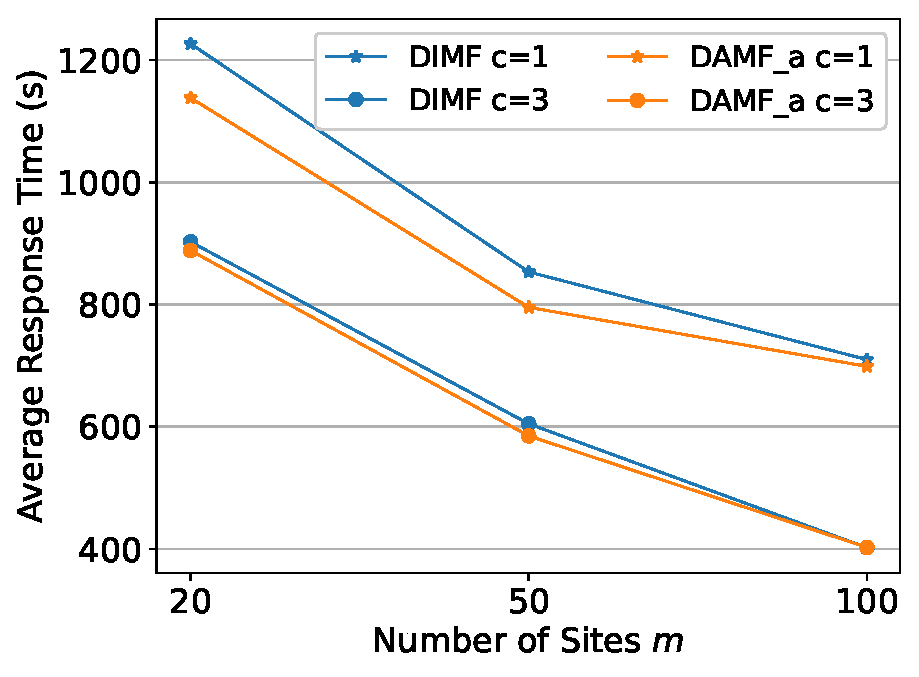
\includegraphics[width=0.48\linewidth]{Image/Workload_Ali2017test_60_site.eps}
    \label{Fg:JRT_Ali_60_m}}

    \caption{Average job response time, Zipf parameter $\alpha=1$.}
    \label{fig:Average_Response_Time_sites}
\end{figure}

\begin{figure}[t]
    \centering
    \subfloat[Alibaba, workload = 40\%]
    {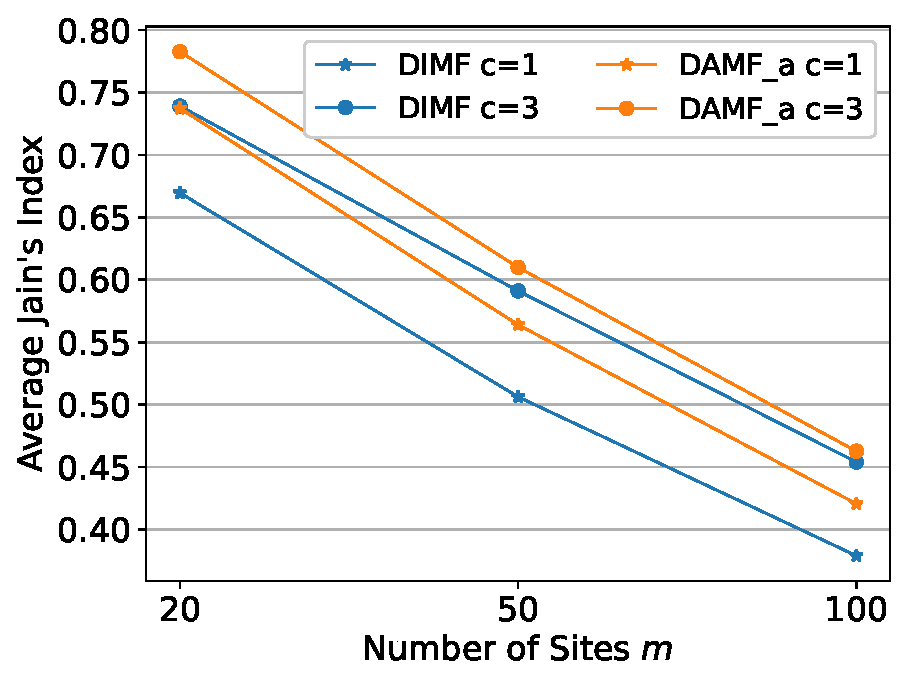
\includegraphics[width=0.48\linewidth]{Image/Jains_Ali2017test_40_site.eps}
    \label{Fg:Jains_Ali_40_m}}
    \hfill
    \subfloat[Alibaba, workload = 60\%]
    {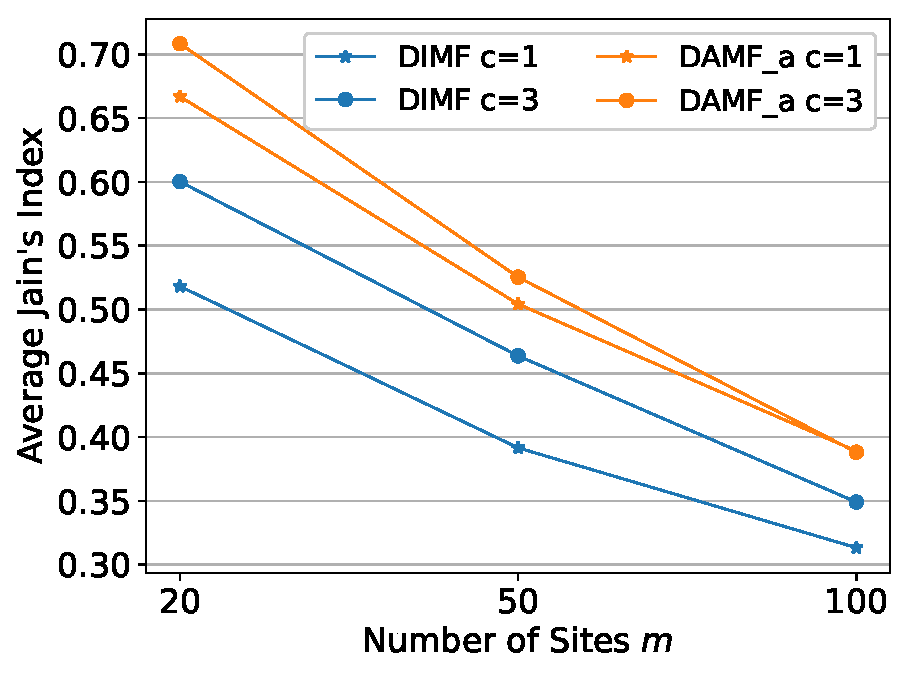
\includegraphics[width=0.48\linewidth]{Image/Jains_Ali2017test_60_site.eps}
    \label{Fg:Jains_Ali_60_m}}

    \caption{Average Jain's Index, Zipf parameter $\alpha=1$.}
    \label{fig:Jains_sites}
\end{figure}

% \begin{table}[!ht]
%   \caption{Average computation time (s) of $\text{DAMF}_a$}
%   \label{tab:computation_time_m}
%   \centering
%   \small 
%   \setlength{\tabcolsep}{4pt} 
%   \begin{tabular}{cc *{6}{S[table-format=1.3e-1]}}
%     \toprule
%     & & \multicolumn{3}{c}{Alibaba, workload = 40\%} & \multicolumn{3}{c}{Alibaba, workload = 60\%} \\
%     \cmidrule(lr){3-5} \cmidrule(lr){6-8} % 画出有间隙的分隔线，更好看
%     $c$ & $\alpha$ & {$m=20$} & {$m=50$} & {$m=100$} & {$m=20$} & {$m=50$} & {$m=100$} \\
%     \midrule
%     \multirow{4}{*}{1} 
%     & 0.0 & 2.035e-5 & 4.908e-5 & 8.455e-5 & 3.732e-5 & 7.321e-5 & 1.594e-4 \\
%     & 0.5 & 2.231e-5 & 4.491e-5 & 7.954e-5 & 3.339e-5 & 6.835e-5 & 1.592e-4 \\
%     & 1.0 & 1.645e-5 & 4.084e-5 & 7.899e-5 & 2.517e-5 & 6.675e-5 & 1.439e-4 \\
%     & 2.0 & 1.586e-5 & 3.561e-5 & 8.723e-5 & 2.243e-5 & 5.335e-5 & 1.219e-4 \\
%     \midrule
%     \multirow{4}{*}{3} 
%     & 0.0 & 2.169e-5 & 4.678e-5 & 9.114e-5 & 3.644e-5 & 7.452e-5 & 1.639e-4 \\
%     & 0.5 & 2.195e-5 & 5.027e-5 & 1.062e-4 & 3.089e-5 & 7.945e-5 & 2.174e-4 \\
%     & 1.0 & 1.836e-5 & 5.408e-5 & 1.137e-4 & 3.035e-5 & 9.177e-5 & 2.428e-4 \\
%     & 2.0 & 1.935e-5 & 5.155e-5 & 1.443e-4 & 2.786e-5 & 9.714e-5 & 2.868e-4 \\
%     \bottomrule
%   \end{tabular}
% \end{table}

\begin{table}[!ht]
  \caption{Average computation time (s) of $\text{DAMF}\_a$}
  \label{tab:computation_time_m}
  \centering
  \resizebox{\columnwidth}{!}{
  \setlength{\tabcolsep}{4pt} 
  \begin{tabular}{cc *{6}{S[table-format=1.3e-2, input-exponent-markers={e}]}}
    \toprule
    & & \multicolumn{3}{c}{Alibaba, workload = 40\%} & \multicolumn{3}{c}{Alibaba, workload = 60\%} \\
    \cmidrule(lr){3-5} \cmidrule(lr){6-8} 
    $c$ & $\alpha$ & {$m=20$} & {$m=50$} & {$m=100$} & {$m=20$} & {$m=50$} & {$m=100$} \\
    \midrule
    \multirow{4}{*}{1} 
    & 0.0 & 2.035e-5 & 4.908e-5 & 8.455e-5 & 3.732e-5 & 7.321e-5 & 1.594e-4 \\
    & 0.5 & 2.231e-5 & 4.491e-5 & 7.954e-5 & 3.339e-5 & 6.835e-5 & 1.592e-4 \\
    & 1.0 & 1.645e-5 & 4.084e-5 & 7.899e-5 & 2.517e-5 & 6.675e-5 & 1.439e-4 \\
    & 2.0 & 1.586e-5 & 3.561e-5 & 8.723e-5 & 2.243e-5 & 5.335e-5 & 1.219e-4 \\
    \midrule
    \multirow{4}{*}{3} 
    & 0.0 & 2.169e-5 & 4.678e-5 & 9.114e-5 & 3.644e-5 & 7.452e-5 & 1.639e-4 \\
    & 0.5 & 2.195e-5 & 5.027e-5 & 1.062e-4 & 3.089e-5 & 7.945e-5 & 2.174e-4 \\
    & 1.0 & 1.836e-5 & 5.408e-5 & 1.137e-4 & 3.035e-5 & 9.177e-5 & 2.428e-4 \\
    & 2.0 & 1.935e-5 & 5.155e-5 & 1.443e-4 & 2.786e-5 & 9.714e-5 & 2.868e-4 \\
    \bottomrule
  \end{tabular}}
\end{table}

\section{Summary}
\label{sec:ch3summary}
In this chapter, we have defined a new resource allocation policy called Dynamic Aggregate Max-min Fairness (DAMF) in distributed job execution with task transmissions. We prove that DAMF satisfies several widely accepted properties, including Pareto efficiency, envy-freeness and strategy-proofness. We present an algorithm for computing the DAMF allocation and a fast approximation. Experimental evaluations using real job traces from Alibaba and Google demonstrate that DAMF could effectively enhance the fairness of resource allocation among jobs and improve the system utility. %In the future, we plan to extend our work to deal with multiple resource types.

% \section*{Acknowledgments}
% This research is supported by the Ministry of Education, Singapore, under its Academic Research Fund Tier 2 (Award MOE-T2EP20121-0005) and Academic Research Fund Tier 1 (Award RG23/23).
\chapter{Task Scheduling and Transmission for Distributed Job Execution}
\label{ch:WAST}


\section{A Motivating Example}
\label{sec:example}

\begin{figure*}[htbp]
    \centering
    % ========== 第一行 ==========
    \begin{subfigure}[t]{0.48\textwidth}
        \centering
        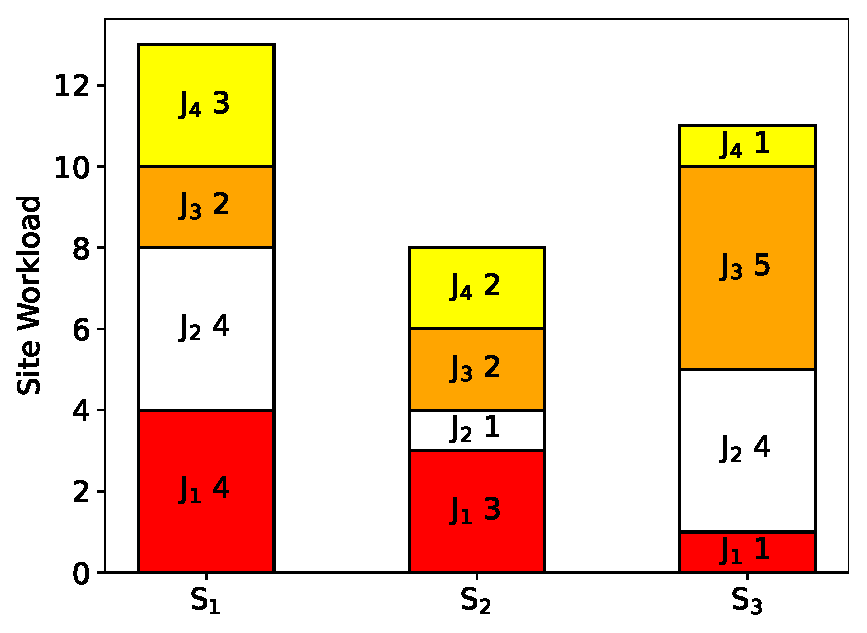
\includegraphics[width=\textwidth]{Image2/Example_1.eps}
        \caption{Indexed Scheduling}
        \label{fig_first_case}
    \end{subfigure}
    \hfill
    \begin{subfigure}[t]{0.48\textwidth}
        \centering
        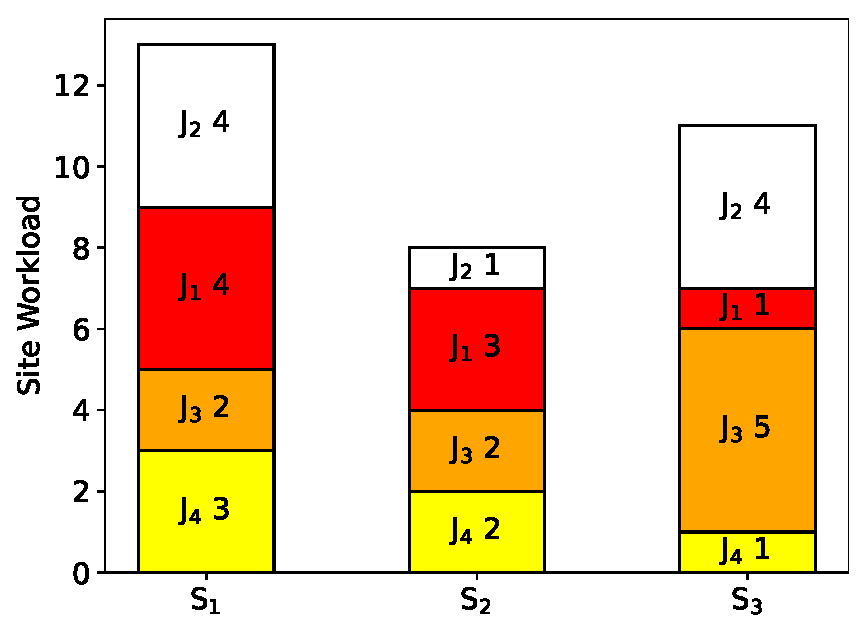
\includegraphics[width=\textwidth]{Image2/Example_2.eps}
        \caption{Optimal Scheduling without Task Transmission}
        \label{fig_second_case}
    \end{subfigure}
    
    \vspace{1.5em} % 👈 这里是关键：空行代表换行，\vspace 增加上下两行之间的间距
    
    % ========== 第二行 ==========
    \begin{subfigure}[t]{0.48\textwidth}
        \centering
        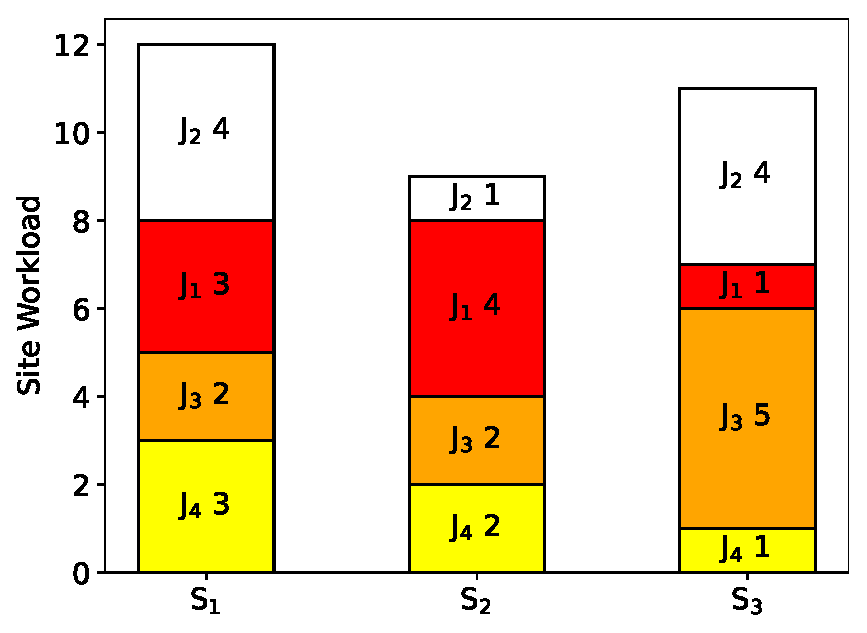
\includegraphics[width=\textwidth]{Image2/Example_3.eps}
        \caption{Optimal Transmission under Execution Order of Fig. \ref{fig_second_case}}
        \label{fig_third_case}
    \end{subfigure}
    \hfill
    \begin{subfigure}[t]{0.48\textwidth}
        \centering
        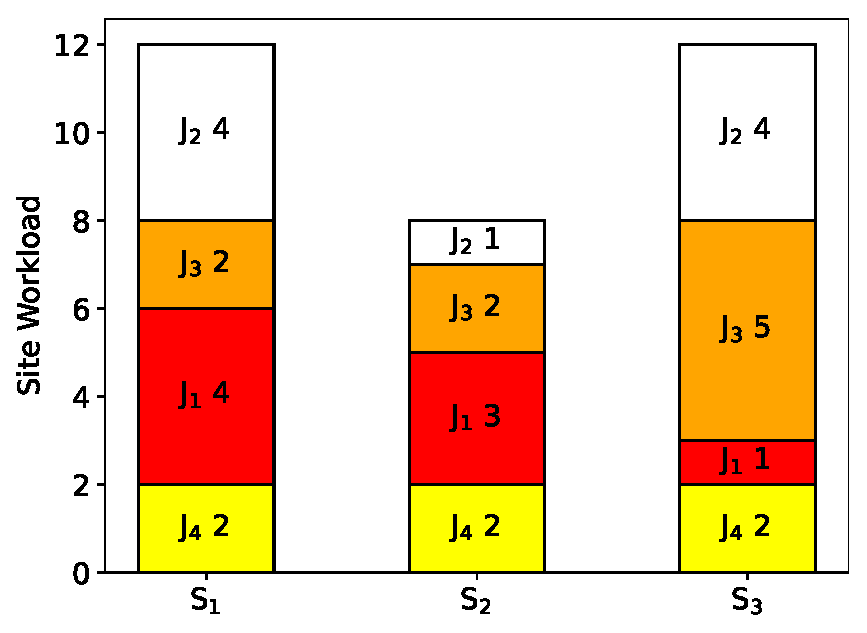
\includegraphics[width=\textwidth]{Image2/Example_4.eps}
        \caption{Optimal Scheduling with Task Transmission}
        \label{fig_fourth_case}
    \end{subfigure}
    
    \caption{Motivating Example} 
    \label{fig:Motivate_example}
\end{figure*}

Fig. \ref{fig:Motivate_example} provides a motivating example of the problem with four jobs $J_1$, $J_2$, $J_3$ and $J_4$ in three geo-distributed data centers (sites) $S_1$, $S_2$ and $S_3$. All jobs are submitted at time $0$. For simplicity, we assume that each task of any job requires one computing slot and takes one time unit to process, and each site has one computing slot only. Fig. \ref{fig_first_case} shows the initial task distribution of each job among the three sites. The response time of a job is decided by the completion time of its last task across all sites. Obviously, different execution orders of the jobs can change the completion times of their tasks and result in different job response times. If the jobs are simply scheduled in the order of their indices (which, for example, represents their submission order), jobs $J_1$, $J_2$, $J_3$ and $J_4$ will complete at time $4$, $8$, $10$ and $13$, respectively, so the total job response time is $4+8+10+13=35$ time units. The optimal job execution order without task transmission is $\langle J_4, J_3, J_1, J_2 \rangle$ as shown in Fig. \ref{fig_second_case}, and the resultant total job response time is $3+6+9+13=31$ time units, which is 4 time units better than the first schedule. 

Suppose that with utilization of network resources, the input data of one task is allowed to be transferred between sites and it takes one time unit to arrive at the destination. Under the job execution order of Fig. \ref{fig_second_case}, the optimal transmission can decrease the total job response time to 29 time units. For example, we can transfer one task of $J_1$ from site $S_1$ to $S_2$, as shown in Fig. \ref{fig_third_case}. This task will arrive at site $S_2$ at time $1$ when the slot of $S_2$ is processing a task of $J_4$ (and $J_4$ is scheduled earlier than $J_1$ in the execution order), so the task transferred can be treated as a local task of $J_1$ at site $S_2$ initially. Consequently, $J_4$, $J_3$, $J_1$ and $J_2$ will complete at time $3$, $6$, $8$ and $12$, respectively, and the total job response time is $3+6+8+12=29$ time units. In our example, the optimal solution is to transfer one task of $J_4$ from site $S_1$ to $S_3$ while modifying the job execution order to be $\langle J_4, J_1, J_3, J_2 \rangle$, as shown in Fig. \ref{fig_fourth_case}. This results in the total job response time of $2+6+8+12=28$ time units, which is even better than the schedule in Fig. \ref{fig_third_case}.

%The problem size (the transmission number limit in particular) of the motivating example is relatively small, and hence the performance disparity among different approaches is not substantial. Nevertheless, it reveals some interesting phenomena. %First, the optimal transmission of the task lies in $J_4$ which has the highest priority. This suggests that jobs with higher priorities in scheduling also tend to have high priorities on network resource usage: transferring out a task at the head of the scheduling queue has higher potential of bringing forward the procession start time of more tasks, which raises the probabilities that some jobs could finish earlier (if their completion times are dependent on their tasks at this site).
%impacting more jobs' completion time at the transmission source site and thereby their global completion time.  at the site where the transmission begins
The above example illustrates some interesting phenomena. First, job execution order and task transmission have mutual influence. The optimal execution order of jobs can change after task transmissions are performed: both execution orders in Figs. \ref{fig_second_case} and \ref{fig_fourth_case} achieve the optimal total job response times given the respective task transmissions, but $J_1$ and $J_3$ are swapped in the execution order after a task is transferred in Fig. \ref{fig_fourth_case}. Vice versa, different job execution orders have different optimal task transmissions: the optimal transmission changes after we modify the job execution order from $\langle J_4, J_3, J_1, J_2 \rangle$ (Fig. \ref{fig_third_case}) to $\langle J_4, J_1, J_3, J_2 \rangle$ (Fig. \ref{fig_fourth_case}). Second, the transmission in the optimal solution is from site $S_1$ to $S_3$, while the site with the lowest load is $S_2$. This indicates that the transmissions that minimize the total job response time can differ from the one that focuses on load balancing, so traditional load balancing techniques may not be preferable in this efficiency-targeted scenario.

\section{System Model}
\label{sec:model}
Consider a system consisting of $m$ separate geo-distributed sites: $\mathcal{S} = \{S_1, S_2, ..., S_m\}$. Each site $S_j$ has compute resources with capacity $u_j$, which can be interpreted as the volume of computing slots available. A set of $n$ jobs $J_1, J_2, ..., J_n$ are submitted to run in the system. Each job $J_i$ consists of tasks that require distinct data partitions and can run in parallel. For simplicity, we assume that each task takes one computing slot to process. In big data processing frameworks, tasks of the same job typically process data partitions of the same size \cite{shvachko2010hadoop, shanahan2015large_spark}, so they would take similar times to process. We denote the processing time of a task in each job $J_i$ as $l_i$, which can be estimated by the historical execution records of the job or sampling-based learning, which proactively samples a small fraction of the tasks in the job to make an estimate~\cite{jajoo2022slearn}.
A job is completed when all of its tasks are completed.

The data partitions required by the tasks of each job are originally distributed among the sites. Due to data locality consideration, each task is initially restricted to be executed at a certain site where its input data is available. Therefore, the computational demand of a job $J_i$ on site $S_j$ can be modeled as the number of its tasks that can run only on $S_j$ initially. We represent the computational demands of all jobs across all sites as a matrix $D_{n \times m}$, where each element $d_{ij}$ denotes job $J_i$'s computational demand on site $S_j$.%\footnote{Throughout this paper, we shall use capital letters to represent matrices as well as arrays, and use the corresponding small letters to stand for the elements therein.} 

Suppose the sites in the system are connected by networks, which can be used to transfer data and hence tasks from one site to another. The network resources in the system is denoted by a matrix $B_{m \times m}$, where each element $b_{ij}$ represents the bandwidth available on the link from site $S_i$ to site $S_j$. $b_{ij}$ is set to 0 if there is no direct link between $S_i$ and $S_j$. Let $r_k$ denote the size of a data partition of job $J_k$, then a task of $J_k$ takes $r_k/b_{ij}$ time to transfer from site $S_i$ to site $S_j$ (if $b_{ij}=0$, this time is defined to be infinite). For simplicity, we assume that the transmissions on each link are carried out sequentially. That is, if there is an ongoing transmission on the link, a new transmission has to wait and its arrival time at the destination site will be delayed.
% then transferring a single task of $J_k$ from site $S_i$ to $S_j$ takes $r_k/b_{ij}$ time
% it takes $r_k/b_{ij}$ time to transfer a single task (and its input data) of $J_k$ from site $S_i$ to $S_j$ (if $b_{ij}=0$, this time is defined to be infinite). 
%  job $J_k$ from site $S_i$ to $S_j$ is $r_k/b_{ij}$ (if $b_{ij}=0$, this time is defined to be infinite). Note that if there are ongoing transmission(s) on the link, a new transmission has to wait and its arrival time will be delayed.
\begin{table}[t]
  \caption{Summary of Notations}
  \label{tab:Notation}
  \centering
  \begin{tabularx}{\linewidth}{lX}
    \toprule
    \textbf{Notation} & \textbf{Definition} \\
    \midrule
    $\mathcal{S} = \{S_1, S_2, \dots, S_m\}$ & Set of sites \\
    $U=\{u_1, u_2, \dots, u_m\}$ & Compute resource capacities of individual sites \\
    $\{J_1, J_2, \dots, J_n\}$ & Set of jobs \\
    $D_{n \times m}$ & Compute resource demands \\
    $B_{m \times m}$ & Network resource availability \\
    $\{l_1, l_2, \dots, l_n\}$ & Task processing times of individual jobs \\
    $\{r_1, r_2, \dots, r_n\}$ & Data partition sizes of individual jobs \\
    \bottomrule
  \end{tabularx}
\end{table}

We study the problem of deriving an execution order of jobs and a set of task transmissions between sites, so that the total job response (completion) time of all jobs is minimized. %\textcolor{red}{Note that the response time of each job is the time span from its arrival (which is a constant) to its completion, so minimizing the total response time is equivalent to minimizing the total completion time.} 
The key notations used in this paper are summarized in Table \ref{tab:Notation}. For simplicity, we use $[x]$ to represent the set $\{1, 2, \dots, x\}$ for a positive integer $x$. Note that although the above model is formulated in a static setting, it can be easily extended to address online scenarios by dynamically capturing snapshots of job demand distributions and system resources. %Here $\langle J_{1}', J_{2}',...,J_{n}'\rangle$ is a sequence where each element $J_{i}'$ denotes the $i$-th job to be processed. $T$ is a three-dimensional matrix and $t_{ijk}$ refers to the number of tasks of $J_i$ to be transferred from $S_j$ to $S_k$. 

\section{Workload-Aware Selection with Transmission}
\label{sec:WAST}

\subsection{Optimizing the Completion Time of a Single Job}
\label{sec:single1}
We start by considering the subproblem of how to utilize network resources in the system to minimize the completion time of a single job. This subproblem can be formulated as follows: Given some workloads and task transmissions already scheduled in the system, and a job $J_k$ with task processing time $l_k$, data partition size $r_k$ and initial demand distribution $d_{k1}, d_{k2}, \dots, d_{km}$ across the $m$ sites, % associated with scheduled jobs from the previous iteration(s)
we would like to determine a set of task transmissions for $J_k$ so that its job completion time can be minimized.
%To describe the state of the system load prior to scheduling $J_k$, we

We use a sequence of arrays $W_1, W_2, \dots, W_m$ to represent the workload already scheduled for each computing slot at each site, where the workload of a slot refers to the total processing time of all tasks assigned to it (i.e., the time when this slot will become available). Each $W_i$ is an array whose length is the number of computing slots at site $S_i$, and each element $w_{ij}$ in $W_i$ represents the scheduled workload of the $j$-th slot at $S_i$. In addition, we use a matrix $T_{m \times m}$ to represent the usage of network resources by the task transmissions already scheduled, where $t_{ij}$ records the time when the link from site $S_i$ to site $S_j$ will complete the scheduled transmissions and become available.% Initially, all $b_{ij}'$s are set to 0. Once a transmission is scheduled, its transmission time will be added to the corresponding entry in $T$.

To avoid the complex interaction between task transmissions and executions and simplify the problem model, we assume that every transferred task will arrive at its destination site before any computing slot at that site becomes available. % \sout{at that site starts to process tasks of subsequent jobs in the execution order}. \sout{This ensures that the tasks of the job (including transferred ones) are processed continuously at each site} 
This ensures that the transferred tasks can be processed continuously at their destination sites together with the tasks originally available there, which simplifies the modeling of job completion time. Based on this, we model the completion time of job $J_k$ as follows. Suppose a matrix $X_{m \times m}$ represents the task transmissions of job $J_k$, where each element $x_{ij}$ refers to how many tasks of $J_k$ are to be transferred from site $S_i$ to site $S_j$. Naturally, each $x_{ij}$ is greater than or equal to $0$. In particular, for each site $S_i$, we define $x_{ii}=0$. We use an array $Y$ of length $m$ to represent the computational demands at the $m$ sites after all the transmissions in $X$ are performed. Each element $y_i$ refers to the number of tasks to be executed at site $S_i$ after the transmissions, and is given by:%. Obviously, the variables in $X$ and $Y$ are integers and for them we have:
\begin{equation}
    \forall i \in [m],\quad y_i = d_{ki} + \sum_{j=1}^m x_{ji} - \sum_{j=1}^m x_{ij}.
\label{eq:constraint1}
\end{equation}

Recall that we assume each task transmission to arrive at its destination site before any computing slot at that site becomes available. Thus, all the $y_i$ tasks of job $J_k$ to be executed at site $S_i$ can be scheduled by iteratively assigning each task to the slot of the lowest workload in $S_i$. Let $w_{ij}^{(t)}$ denote the workload of the $j$-th slot in site $S_i$ after $t$ tasks of $J_k$ are assigned to the slots at $S_i$. $w_{ij}^{(t)}$ can be computed iteratively as follows:% \[
% \begin{aligned}
% \text{Initialization: }&\forall j \in [u_i], \text{ } w_{ij}^{(0)} = w_{ij},\\
% \text{for each } & t = 1, \;2, \;\dots, \;y_i:\\
% %\text{find the slot $p$ with the lowest workload: }\\
% %p = \text{any } &\text{element of }\argmin_{1 \le j \le u_i} w_{ij}^{(t-1)}, \\
% \forall j \in [u_i],& w_{ij}^{(t)} =
% \begin{cases}
% w_{ij}^{(t-1)} + l_k, & j = \argmin_{1 \le p \le u_i} w_{ip}^{(t-1)}, \\
% w_{ij}^{(t-1)}, & else.
% \end{cases} \\
% \end{aligned}
% \]
%\begin{equation*}
%\forall j \in [u_i], \text{ } w_{ij}^{(0)} = w_{ij},
%\end{equation*}
\begin{multline}
\!\!\!\!\!\!\forall j \in [u_i], \;\;\; 
w^{(t)}_{ij} =
\begin{cases}
w_{ij}, \qquad \qquad \, t=0 \\
w^{(t-1)}_{ij} + l_k, 
\;\;\; j = \argmin_{p \in [u_i]} w^{(t-1)}_{ip}, \\
w^{(t-1)}_{ij}, 
\qquad \;\;\; j \neq \argmin_{p \in [u_i]} w^{(t-1)}_{ip}, 
\end{cases}
\nonumber
\end{multline}
where in each iteration, a task is assigned to the slot of the lowest workload ($\argmin_{p \in [u_i]} w_{ip}^{(t-1)}$) and its workload then increases by $l_k$, while other slots are kept unchanged. Ties are broken arbitrarily if multiple slots have the same lowest workload.
Based on this, the time when all $y_i$ tasks complete execution at site $S_i$ can be estimated as a function $f(W_i, y_i)$:
\[
f(W_i, y_i) =
\begin{cases}
0, & y_i = 0, \\
\min_{j \in [u_i]}(w_{ij}^{(y_i-1)})+l_k,  & y_i > 0,
\end{cases}
\]
which gives the completion time of the last task at $S_i$.
Note that function $f$'s inputs and outputs cannot be captured by any closed-form expression. %Therefore, given any $y_i$, the completion time of all $y_i$ tasks at site $S_i$ can be derived based on the computation above. 
The objective of optimizing the job completion time of $J_k$ (i.e., $\max_{i \in [m]} f(W_i,y_i)$ --- the completion time of its last task across all sites) can be achieved by searching for the best task transmissions $X$ between sites, which decide the computational demands $Y$ at different sites and hence job $J_k$'s completion time. 
%Not working: Here we suppose tasks are added one slot by one slot.
%If there is a deep low workload at some slot, it may need multiple tasks to be added to it consecutively.
%In this circumstance, given how many tasks are present at a site $S_i$ (tasks transferred from other sites will arrive at the time when all local slots are still busy processing tasks of jobs with prior execution order or tasks of the same job, thus they could be treated in a similar way as local demand), we could add tasks  using a step-by-step manner, and the estimated job response time on a site $S_i$ can be expressed as follows:
%derive the resultant job response time on $S_i$ given any $Y_i$: %WLOG, suppose the computing slots in $S_i$ has a non-decreasing workload $W_{i0} \leq W_{i1} \leq ...... \leq W_{iU_i}$, then the estimated job response time on site $S_i$ is a integer function of $Y_i$:


%It is important to determine the bound of $X$ and $Y$ before searching starts, and there are multiple factors restricting the bounds. Suppose that the current job is $J_k$: first, a transmission could start only if there is existing demand on the site, so each $x_{ij}$ and $y_i$ has a lower bound $-d_{ki}$; second, transmission could only happen when the starting site's estimated local JRT is larger than that of the destination site, because a valid transmission will narrow instead of deteriorate the gap of local JRT between any two sites. This restricts the upper limit on half of the elements in $X$ to be zero and lower limit to be zero on the other half. Third, to ensure that a transmission will arrive in time, the existing transmission delay of the link plus the unit transmission time cost should be less than or equal to the minimum workload of the slot in the destination site. This further controls the upper limit of the elements in $X$. Finally, each site could receive tasks as long as its local JRT is still smaller than the global JRT without transmission, which gives upper bounds on each element in $Y$. Together, these constraints derive the upper and lower bounds of $X$ and $Y$; To facilitate the representation, we use $A$ and $C$ to record the upper bound in $X$ and $Y$, respectively. The algorithm \ref{alg:Single1} describes the basic approach to find the minimum JRT that current job $J_k$ is possible to reach. The algorithm first computes the lower and upper bounds for variables in $X$ and $Y$ as well as the estimated local JRT given how many tasks are added to or removed from each site, then start a program to minimize the maximum local JRT, a.k.a., global JRT.

It is essential to determine the bounds of $X$ before starting the search. 
%as they are restricted by multiple factors. 
An excessively tight bound can limit the potential benefit of task transmissions in reducing the job completion time, whereas an excessively loose bound may give rise to task transmissions that fail to reach the destination sites in time, thereby introducing additional delays in the job completion time. %As discussed, we \textcolor{red}{hope} each task to arrive at its destination site when no computing slot of that site has started processing the subsequent jobs. \sout{, and we require it to be no later than the lowest workload among all slots after $d_{kj}+x_{ij}-1$ tasks are assigned to $S_j$. Such modeling of the task transmission requirement assumes that at least $d_{kj}$ tasks are present at the destination site $S_j$ when the first transmission from site $S_i$ arrives, and does not account for potential task transmissions out of site $S_j$ as well as transmissions to site $S_j$ from sites other than $S_i$}
%the arrival time of the last transmission is $t_{ij} + x_{ij}\cdot r_k/b_{ij}$, and 
Suppose $x_{ij}$ tasks are to be transferred from site $S_i$ to site $S_j$. Then, the completion time of the last task will be at least $t_{ij} + x_{ij}\cdot r_k/b_{ij} + l_k$ (when it is processed immediately after arrival), and we require this last task to finish before the job completion time:
\begin{multline}
\forall i \in [m], \; j \in [m], \;
t_{ij} + \frac{x_{ij} \cdot r_k}{b_{ij}} + l_k \le \max_{i \in [m]} f(W_i,y_i).
\label{eq:constraint_t}
\end{multline}

In addition, the number of tasks transferred out of a site cannot exceed the number of tasks it holds initially, which imposes another upper bound on $\sum_{j=1}^m x_{ij}$ at each site $S_i$:
\begin{equation}
    \forall i \in [m], \quad 0 \leq \sum_{j=1}^m x_{ij} \leq d_{ki}.
\label{eq:constraint_sum}
\end{equation}
%Constraint (\ref{eq:constraint_sum}) ensures that the sum of the first and third terms ($d_{ki} -\sum_{j=1}^m x_{ij}$) in equation (\ref{eq:constraint1}) is nonnegative, which provides implicit guarantees that the elements in $Y$ are nonnegative. 

Constraints (\ref{eq:constraint_t}) and (\ref{eq:constraint_sum}) collectively define the upper bounds of the elements in $X$. Therefore, we can define a program to search for task transmissions $X$ under constraints (\ref{eq:constraint1}), (\ref{eq:constraint_t}) and (\ref{eq:constraint_sum}) to optimize the job completion time $\max_{i \in [m]} f(W_i,y_i)$. %which decides the number of tasks after transmissions on each site $Y$, and hence job $J_k$'s response time (using function $f$). }% Since each element in $Y$ is a linear combination of some elements in $X$, its upper bounds are implicitly determined by $X$.
%Second, a valid transmission should only reduce the disparities between the task completion times at different sites. Hence, transmissions should not be performed from site $S_i$ to site $S_j$ if the estimated task completion time at the source site $f(S_i, d_{ki})$ is no later than that at the destination $f(S_j, d_{kj})$ when all tasks are processed without transmissions. This imposes an upper bound of zero on half of the elements in $X$:
%The constraints (\ref{eq:constraint_Xbound}), (\ref{eq:constraint3}) and (\ref{eq:constraint4}) above collectively define the feasible upper bounds of elements in $X$. Since each element in $Y$ is a linear combination of some elements in $X$, its upper bound are implicitly determined by $X$. %For notational convenience, we denote the upper bounds of $X$ derived by the constraints above as a matrix $A$, where each element $a_{ij}$ represents the upper bound of $x_{ij}$ in $X$:
If multiple transmission matrices $X$'s produce the same minimum job completion time, we choose the $X$ with the least total number of task transmissions. The rationale is to minimize the network resource usage and make more network resources available to other jobs.
% with minimized $\sum_{i=1}^m \sum_{j=1}^m x_{ij}$ are returned.

%If any $Y_i=0$, the resultant JRT of $S_i$ is its initial local JRT. Similarly, initially, the local demand of current job across all sites could be simply placed one by one(note that with the principle mentioned above, there is no need to consider transmissions of jobs with higher priority, because they must have arrived and been in process before tasks of the current job start to proceed), each time selecting the slot with the lowest workload. After this, we could obtain the estimated local JRT of the current job across each site. We define a transmission using a tuple $E(J_i, S_j, S_k)$, representing a transmission's belonging job, start site and destination site, respectively. A valid transmission should satisfy some basic conditions: 

\subsection{Transformation into ILP}
\label{sec:transformation}
The program in Section \ref{sec:single1} cannot be solved directly by popular optimization solvers owing to the discrete function $f$, which 
%As mentioned previously, due to various workload conditions at different sites, the relationship between $f$'s inputs and outputs 
cannot be captured by any closed-form expression. % For example, after a task is assigned to some site $S_j$, it is possible that the task completion time of $S_j$ increases or remains unchanged. 
%seems to provide a complete solution for the single-job case. However, it
In order to make the program solvable, we transform it into solving multiple Integer Linear Programs (ILP) that are supported by popular solvers. To facilitate presentation, we refer to the completion time of the last task at a site $S_i$ as "the completion time at site $S_i$". We compute and record the completion times $f(W_i, y_i)$ at each site $S_i$ using the method introduced in Section \ref{sec:single1}, for increasing number of tasks $y_i$ scheduled at site $S_i$ starting from $y_i=0$. %\sout{In particular, $f(W_i, 0)$ is set to 0 for each site $S_i$.} 
The calculation ends at the lowest $y_i$ value where the resulting $f(W_i, y_i)$ at site $S_i$ exceeds the job completion time when all tasks are executed locally without transmission, i.e., $\max_{i\in[m]}f(W_i, d_{ki})$. 

Note that these $f(W_i, y_i)$ values include all possible completion times at each site that $J_k$ can produce, and they are non-decreasing with respect to $y_i$ since adding a new task can never reduce the completion time at a site. With these $f(W_i, y_i)$ values, given any target job completion time $z$, the maximum number of tasks $c_i$ that each site $S_i$ can process (to keep its completion time within this target) can be derived as $c_i = \max\{p \mid f(W_i, p)\leq z\}$. Thus, the target $z$ can be converted to an array of upper bounds $c_1, c_2, \dots, c_m$ for the elements $y_1, y_2, \dots, y_m$ in $Y$. Hence, the problem of determining ``whether the job $J_k$ can achieve a target job completion time $z$ using task transmissions'' can be transformed to determining whether task transmissions can be performed to bound the elements in $y_1, y_2, \dots, y_m$ by $c_1, c_2, \dots, c_m$. The latter can be formulated as an ILP, because its constraints are linear and the elements in $X$ and $Y$ are integers. Furthermore, the minimum job completion time that $J_k$ can achieve must be among all the $f(W_i, y_i)$ values. Therefore, we can sort all values $f(W_1, 0)$, $f(W_1, 1), \dots, f(W_1, c_1), f(W_2, 0), f(W_2, 1), \dots, f(W_2, c_2)$, $\dots, f(W_m, 0), f(W_m, 1), \dots, f(W_m, c_m)$ to form an array $\psi$. Then, the minimum job completion time of $J_k$ can be found by a binary search in $\psi$ and solving multiple ILPs.
%In this circumstance, the result $P_{it}$ is discarded, and the computation for the site ends.% Once after a new task is added to a site and the corresponding job response time exceeds the threshold,
%We compute the completion times at each site given different numbers of tasks and record them in $m$ arrays, namely $P_1, P_2, \dots, P_m$. More specifically, each element $p_{ij}$ records the completion time at site $S_i$ if $j$ tasks of $J_k$ are processed at $S_i$. \textcolor{red}{The first element $p_{i0}$ of each array $P_i$ is set to 0.} The method of computing the array $P_i$ is based on the approach used for calculating $w_{ij}^{(t)}$s in Section \ref{sec:single1}. We record $\min_{1\leq j \leq u_i}w_{ij}^{(t-1)} + l_k$ for each $t=1, 2,\dots$ as $p_{it}$. The computation ends at the lowest $t$ value where the resulting completion time $\min_{1\leq j \leq u_i}w_{ij}^{(t-1)} + l_k$ at site $S_i$ exceeds the original job response time (i.e., the job response time when all tasks are executed locally without transmission). %In this circumstance, the result $P_{it}$ is discarded, and the computation for the site ends.% Once after a new task is added to a site and the corresponding job response time exceeds the threshold,

%Note that the array set $P_1, P_2, \dots, P_m$ stores all possible completion times at each site that $J_k$ can produce, and each array is guaranteed to be non-decreasing with respect to their indices since adding a new task can never reduce the completion time at a site. With this array set, given any target job response time $z$, the maximum number of tasks that a site $S_i$ can process (to keep its corresponding completion time within this target) can be derived by checking array $P_i$. \textcolor{red}{More specifically, suppose that the number of elements of array $P_i$ is $P_i.size$, this maximum number is $\argmax_{0\leq j < P_i.size}p_{ij}\leq z$.} Thus, the target can be converted to an array of upper bounds $c_1, c_2,\dots,c_m$ for the elements $y_1, y_2, \dots, y_m$ in $Y$. Hence, the problem "whether the job $J_k$ could achieve this target job response time using task transmissions" is equivalent to determining whether task transmissions can be performed to bound the elements in $Y$ by $C$. The latter can be formulated as an ILP, because its constraints are linear and the elements in $X$ and $Y$ are integers. Furthermore, the minimum job response time that $J_k$ can achieve must be in the array set $P_1, P_2, \dots, P_m$. Therefore, we can consolidate all elements in $P_1, P_2, \dots, P_m$, eliminate duplicates if any, and sort them to derive an array $\psi$, and the minimum job response time of $J_k$ can be found by a binary search in $\psi$ and solving multiple ILPs.%(note that by the transformation above we eliminated constraints using function $f$)


%is the optimal solution $J_k$ could possibly achieve. Every entry in $Y$ should at

%that fall below the minimum local JRT are discarded, as they are irrelevant or infeasible. We then utilize binary search to obtain the minimum JRT bound from $JRT_p$ and return the transmission $X$ under this JRT bound. By such modification, we replace Algorithm \ref{alg:Single1} with a series of ILP instances to efficiently identify the minimum achievable JRT for $J_k$. The procedure is elaborated in Algorithm \ref{alg:Single2}. 
% 请确保在 LaTeX 文件的导言区（Preamble）引入了该宏包：
% \usepackage[linesnumbered,ruled,vlined]{algorithm2e}

\begin{algorithm}[t]
\caption{Optimizing the Completion Time of a Single Job}\label{alg:Single2}

    \KwIn{A set of sites $\mathcal{S}$ with compute capacities $U$ and network resources $B$; a job $J_k$ to be scheduled with task processing time $l_k$, data partition size $r_k$ and computational demand distribution $d_{k1}, d_{k2}, \dots, d_{km}$; current workload $W_1, W_2, \dots, W_m$ and network usage $T$;}
    \KwOut{$J_k$'s optimal job completion time and task transmissions;}
    \BlankLine

    Compute and record $f(W_i, y_i)$'s for each site $S_i$ with increasing $y_i$ until $f(W_i, y_i) \geq \max_{i\in[m]}f(W_i, d_{ki})$, using the method in Section \ref{sec:single1}\;
    Merge and sort all $f(W_i, y_i)$ values to form an array $\psi$\;
    % Collect all possible task completion times that each site can reach, record them in arrays $P_1, P_2, \dots, P_m$; merge and sort them into an array $\psi$; remove duplicate elements from $\psi$;
    $low=1$; $high=\psi.size$; $opt = 0$\;
    \BlankLine

    \While{$low < high$}{
        $middle = \lfloor (low + high)/2\rfloor$\;
        $c_i = \max\{p \mid f(W_i, p)\leq \psi[middle]\}$, for each $i \in [m]$\;
        \BlankLine
        
        Minimize $\sum_{i=1}^m\sum_{j=1}^m x_{ij}$, subject to:\;
        \quad $\forall i \in [m], j \in [m],\; t_{ij} + \frac{x_{ij}*r_k}{b_{ij}} + l_k \leq \psi[middle]$;\;
        \quad $ \forall i \in [m],\; 0 \leq \sum^m_{j=1}x_{ij} \leq d_{ki}$;\;
        \quad $ \forall i \in [m],\; y_i = d_{ki} + \sum_{j=1}^m x_{ji} - \sum_{j=1}^m x_{ij}$;\;
        \quad $\forall i \in [m],\; y_i \leq c_i$;\;
        \quad all $x_{ij}$'s and $y_i$'s are non-negative integers;\;
        \BlankLine
        
        \eIf{the above ILP is feasible and admits a solution}{
            $opt = \psi[middle]$\;
            $X \leftarrow x_{ij}$'s in the solution of the above ILP\;
            $high = middle - 1$\;
        }{
            $low = middle + 1$\;
        }
    }
    \BlankLine
    \Return $opt$, $X$\;
\end{algorithm}

% \begin{algorithm}[t]
% \caption{Optimizing the Completion Time of a Single Job}
% \label{alg:Single2}
% \begin{algorithmic}[1]
% \STATE \textbf{Input}: A set of sites $\mathcal{S}$ with compute capacities $U$ and network resources $B$; a job $J_k$ to be scheduled with task processing time $l_k$, data partition size $r_k$ and computational demand distribution $d_{k1}$, $d_{k2}, \dots, d_{km}$; current workload $W_1, W_2, \dots, W_m$ and network usage $T$;
% \STATE \textbf{Output}: $J_k$'s optimal job completion time and task transmissions;
% \STATE \textbf{Initialization}: Compute and record $f(W_i, y_i)$'s for each site $S_i$ with increasing $y_i$ until $f(W_i, y_i) \geq \max_{i\in[m]}f(W_i, d_{ki})$, using the method in Section \ref{sec:single1}; merge and sort all $f(W_i, y_i)$ values to form an array $\psi$;%Collect all possible task completion times that each site can reach, record them in arrays $P_1, P_2, \dots, P_m$; merge and sort them into an array $\psi$; remove duplicate elements from $\psi$; %remove elements below the ideal bound derived under the infinite bandwidth assumption from $\psi$. 
% % \STATE Compute $X$'s upper bound $A$ based on the following constraints:
% % \STATE$\forall i \in [m], j \in [m]: 0 \leq x_{ij} \leq d_{ki}$;
% % \STATE$\forall i \in [m], j \in [m]: f(S_i,d_{ki}) \leq f(S_j, d_{kj}) \xrightarrow{} x_{ji} \leq 0$;
% % \STATE$\forall i \in [m], j \in [m]: T_{ij} + \frac{x_{ij}*r_k}{b_{ij}} \leq \min(w^{\max(0, (x_{ij}-1))}_j)$;
% \STATE $low=1$; $high=\psi.size$; $opt = 0$;
% \WHILE {$low < high$}
% \STATE $middle = \lfloor (low + high)/2\rfloor$;
% \STATE $c_i = \max\{p \mid f(W_i, p)\leq \psi[middle]\}$, for each $i \in [m]$;%Update $Y$'s upper bound $C$ based on $\psi_{middle}$ and $P_1, P_2, \dots, P_m$;
% \STATE Minimize $\sum_{i=1}^m\sum_{j=1}^m x_{ij}$, subject to:
% %\STATE \quad Minimize $max\_JRT$, subject to:
% %\STATE $\quad \forall i \in [m]: max\_JRT \geq JRT(y_i)$;

% %\STATE \quad$ \forall i \in [m], j\in [m]: 0 \leq x_{ij} \leq a_{ij}$;
% \STATE \quad $\forall i \in [m], j \in [m],\; t_{ij} + \frac{x_{ij}*r_k}{b_{ij}} + l_k \leq \psi[middle]$;
% \STATE \quad$ \forall i \in [m],\; 0 \leq \sum^m_{j=1}x_{ij} \leq d_{ki}$;
% \STATE \quad$ \forall i \in [m],\; y_i = d_{ki} + \sum_{j=1}^m x_{ji} - \sum_{j=1}^m x_{ij}$;
% \STATE \quad $\forall i \in [m],\; y_i \leq c_i$;
% \STATE \quad all $x_{ij}$'s and $y_i$'s are non-negative integers; 
% % \STATE \quad $\forall i \in [m], j \in [m], x_{ij} \in N^+$
% \IF{the above ILP is feasible and admits a solution}
% \STATE $opt = \psi[middle]$;
% \STATE $X \leftarrow x_{ij}$'s in the solution of the above ILP;
% \STATE$high = middle - 1$;
% \ELSE
% \STATE$low = middle + 1$;
% \ENDIF
% \ENDWHILE
% \STATE \textbf{return} $opt$, $X$;
% \end{algorithmic}
% \end{algorithm}

\begin{figure}[htbp]
  \centering
  %\resizebox{\linewidth}{!}{
\begin{tikzpicture}
[
    scale=0.65, 
    transform shape,
    %transform shape=false,
    % node distance=10mm and 22mm,
    % rect/.style={draw, rounded corners, minimum width=14mm, minimum height=9mm, align=center},
    % s/.style={circle, draw, thick, minimum size=9mm, align=center},
    % edge/.style={-Stealth, thick},
    % labsmall/.style={font=\small}
    node distance=1.5em and 3em,
    rect/.style={draw, rounded corners, minimum width=4em, minimum height=2.5em, align=center, font=\normalsize},
    s/.style={circle, draw, thick, minimum size=2.5em, align=center,, font=\normalsize},
    edge/.style={-Stealth, thick},
    labsmall/.style={font=\small}
]

% --- nodes: source, tasks (with vdots), sites (with vdots), sink

\node[rect] (SS1) {$S_1^{out}$};
\node[rect, below=of SS1] (SS2) {$S_2^{out}$};
\node[rect, below=of SS2] (SS3) {$S_3^{out}$};
\node[s, left=28mm of SS3] (s) {$s$};
\node[font=\Large, below=of SS3] (Tdots) {$\vdots$};
\node[rect, below=of Tdots] (SSm) {$S_m^{out}$};

\node[rect, right=35mm of SS1] (S1) {$S_1^{in}$};
\node[rect, below=of S1] (S2) {$S_2^{in}$};
\node[rect, below=of S2] (S3) {$S_3^{in}$};
\node[font=\Large, below=of S3] (Sdots) {$\vdots$}; 
\node[rect, below=of Sdots] (Sm) {$S_m^{in}$};
\node[s, right=28mm of S3] (t) {$t$};

% --- dashed vertical separators (optional, 改坐标可调整高度)
% \draw[dashed] ($(s)+(16mm,28mm)$) -- ($(s)+(16mm,-44mm)$);   % between source and T
% \draw[dashed] ($(S1)+(16mm,28mm)$) -- ($(S1)+(16mm,-44mm)$); % between S and sink

% --- edges: source -> tasks
\draw[edge] (s) -- (SS1) node [midway, above, sloped] {$d_{k1}$};
\draw[edge] (s) -- (SS2) node [midway, above, sloped] {$d_{k2}$};
\draw[edge] (s) -- (SS3) node [midway, above, sloped] {$d_{k3}$};
\draw[edge] (s) -- (SSm) node [midway, above, sloped] {$d_{km}$};

% --- edges: tasks -> sites (示例连接，按需改/增)
\draw[edge] (SS1) -- (S1);
\draw[edge] (SS1) -- (S2);
\draw[edge] (SS1) -- (S3);
\draw[edge] (SS2) -- (S1);
\draw[edge] (SS2) -- (S2);
\draw[edge] (SS2) -- (S3);
\draw[edge] (SS3) -- (S1);
\draw[edge] (SS3) -- (S2);
\draw[edge] (SS3) -- (S3);
\draw[edge] (SSm) -- (Sm);

% --- edges: sites -> sink
\draw[edge] (S1) -- (t)node [midway, above, sloped] {$c_{1}$};
\draw[edge] (S2) -- (t)node [midway, above, sloped] {$c_{2}$};
\draw[edge] (S3) -- (t)node [midway, above, sloped] {$c_{3}$};
\draw[edge] (Sm) -- (t)node [midway, above, sloped] {$c_{m}$};

\end{tikzpicture}
%}
\caption{The flow network}
\label{fig:flow_network}
\end{figure}

Algorithm \ref{alg:Single2} presents the details of optimizing the job completion time of job $J_k$. $\psi.size$ represents the number of elements in the array $\psi$. The algorithm first computes and records the possible completion times $f(W_i, y_i)$ at each site $S_i$ using the method introduced in Section \ref{sec:single1}. These values are then merged and sorted to form a new array $\psi$ which records the job completion times that $J_k$ can possibly achieve. Next, a binary search is applied to the array $\psi$ to find the optimal job completion time in $\psi$ as well as the transmissions required. The parameters $low$ and $high$ in the algorithm refer to the boundary indices of the binary search. In each iteration, the $middle$ index and bounds $c_1, c_2, \dots, c_m$ are updated, and the feasibility of an ILP is checked to decide whether the job completion time $\psi[middle]$ is achievable.
%, and elements that are either duplicated or below a certain threshold are removed from $JRT\_p$ to reduce computation overhead. Next, a binary search method is applied to $JRT\_p$ so that each time a time threshold in $JRT\_p$ is located. The upper bound $C$ of entries in $Y$ are updated using the threshold, and a new ILP is constructed to decide whether this threshold is achievable. After the binary search, the optimal job response time as well as the required transmission(s) can be found. Details of the algorithm are elaborated in Algorithm \ref{alg:Single2}. The parameters $low$ and $high$ in the algorithm refer to the left and right boundary indices of the binary search. $JRT\_p.size$ returns the number of elements in $JRT\_p$., during which elements duplicated and elements that fall below the ideal lower bound are removed

\subsection{Transformation into Minimum-cost Flow Problem}
\label{sec:flow}


% \begin{figure}[htbp]
%     \centering
% \includegraphics[width=\linewidth]{flow_network.tikz}
%     \caption{The flow network}
%     \label{fig:flow_network}
% \end{figure}
\begin{comment}
\begin{algorithm}[htbp]
\caption{Optimizing the Completion Time of a Single Job}
\label{alg:Single3}
\begin{algorithmic}[1]
\STATE \textbf{Input}: A set of sites $\mathcal{S}$ with compute capacities $U$ and network resources $B$; a job $J_k$ to be scheduled with task processing time $l_k$, data partition size $r_k$ and computational demand distribution $d_{k1}$, $d_{k2}, \dots, d_{km}$; current workload $W$ and network usage $T$;
\STATE \textbf{Output}: $J_k$'s optimal job response time and transmissions;
\STATE \textbf{Initialization}: Compute and record $f(W_i, y_i)$'s for each site $S_i$ with increasing $y_i$ until $f(W_i, y_i) \geq \max_{i\in[m]}f(W_i, d_{ki})$, using the method in Section \ref{sec:single1}; merge and sort all $f(W_i, y_i)$ values to form an array $\psi$; %remove elements below the ideal bound derived under the infinite bandwidth assumption from $\psi$. 

\STATE $low=1$; $high=\psi.size$; $opt = 0$;
\While {$low < high$}
\STATE $middle = \lfloor (low + high)/2\rfloor$;
\STATE $c_i = \max\{p \mid f(W_i, p)\leq \psi[middle]\}$, for each $i \in [m]$;
%\STATE Update the capacity of edge $(S^{in}_i, t)$ to be the new $c_i, i=1,2,\dots, m$;
\STATE Construct the flow network for $J_k$;
\STATE Solve the flow network while minimize the flow cost;
\If{the above flow network admits a total flow of $\sum_{i=1}^m d_{ki}$ units}
\STATE $opt = \psi[middle]$;
% \For {$i \in [m], j \in[m], j \neq i$}
% \STATE $x_{ij}=$ flow of edge $(S_i^{out}, S_j^{in})$;
% \EndFor
\STATE $x_{ij}=$ the flow amount on edge $(S_i^{out}, S_j^{in})$, for each $i,j \in [m]$ and $i \neq j$;
\STATE $x_{ii}=0$, for each $i \in [m]$;
\STATE$high = middle - 1$;
\Else
\STATE$low = middle + 1$;
\EndIf
\EndWhile
\STATE \textbf{return} $opt$, $X$;
\end{algorithmic}
\end{algorithm}
\end{comment}
%can be examined from a slightly different perspective: Each site $S_i$ has an initial number of tasks $d_{ki}$, and the number of tasks that each site could transfer to another site $S_j$ has an upper limit denoted by $t_{ij} + \frac{x_{ij}*r_k}{b_{ij}} \leq \min(w^{(d_{kj}+x_{ij}-1)}_j)$. The question is to find a set of transmissions so that site $S_i$'s final number of task $y_i$ falls below $c_i$. the objective becomes to find a set of flows that fall below their corresponding flow capacities (including the capacities for each link in the network and capacities for each site $c_i$). 

Algorithm \ref{alg:Single2} solves the problem, but its computational complexity could raise concerns. 
%Under the transformation in the last section, the problem of searching for the minimum job response time of a single job is decomposed into multiple ILP feasibility problems, which 
ILP is NP-hard in general. If the solution space becomes huge (e.g., the job has thousands of tasks unevenly spread across tens of geo-distributed sites), solving the ILP can incur intolerable computational overhead. To improve the algorithm's efficiency, we further transform the ILP problem in lines 8-13 of Algorithm \ref{alg:Single2} to a minimum-cost flow problem in a bipartite flow network shown in Fig.~\ref{fig:flow_network}. The flow network has a source node $s$, a sink node $t$, a set of $m$ nodes on the left side and a set of $m$ nodes on the right side. To facilitate exposition, we use $S^{out}_i$ and $S^{in}_i$ to represent the $i$-th node on the left and right sides, respectively. A set of $m$ edges with cost 0 connects the source node $s$ to the $m$ nodes on the left, and the capacity of each edge $(s, S_i^{out})$ is set to $d_{ki}$. In addition, a set of $m\times m$ edges connects the $m$ nodes on the left to the $m$ nodes on the right. The capacity of each edge $(S_i^{out},S_j^{in})$ where $i\neq j$ is set to the upper bound of $x_{ij}$ given in line 9 of Algorithm \ref{alg:Single2} (where $\psi[middle]$ is the target job completion time) and the cost of the edge is set to 1. The capacity of each edge connecting each pair of nodes with the same index $(S^{out}_i, S^{in}_i)$ is set to $d_{ki}$ (the initial computational demand at site $S_i$) and the cost of the edge is set to 0. Finally, a set of $m$ edges with cost 0 connect the $m$ nodes on the right to the sink node $t$, and the capacity of each edge $(S^{in}_i, t)$ is set to $c_i$ (the upper bound of $y_i$ for the target job completion time). The problem is to decide whether the bipartite flow network can transfer all $\sum_{i=1}^m d_{ki}$ units of flows from $s$ to $t$ under the given edge capacity constraints while minimizing the total cost. 
%Algorithm \ref{alg:Single3} presents the details.% (note that each $c_i$ changes as the binary search proceeds)

%In the algorithm, we again conduct a binary search in the array $\psi$ to derive the upper limit on the number of tasks that each site can execute. This limit is used to set the capacities of the edges connecting each node $S^{in}_i$ and the sink node $t$. 
Each edge $(s, S^{out}_i)$ represents the initial number of tasks $d_{ki}$ at site $S_i$. Each edge $(S_i^{out},S_j^{in})$ where $i \neq j$ denotes the task transmissions from site $S_i$ to site $S_j$. Due to the flow conservation constraint, the sum of flows going out of each node $S_i^{out}$ is $d_{ki}$, ensuring that the number of task transmissions out of site $S_i$ does not exceed $d_{ki}$. Each edge $(S_i^{out},S_i^{in})$ denotes the number of local tasks that are not transferred out of site $S_i$, so it refers to no transmission and the cost is set to 0. Each edge $(S^{in}_i, t)$ represents the final number of tasks to be executed at site $S_i$ after transmissions, which is required to fall below the upper bound $c_i$. It is easy to verify that this minimum-cost flow problem is equivalent to the ILP problem in Section \ref{sec:transformation}. Since all the edge capacities in the flow network are integers, based on the Integral Flow Theorem \cite{lawler2001combinatorial}, the solution (if it exists) is made up of integral units of flows on all edges. Existing algorithms (e.g., Successive Shortest Path Algorithm, Cost Scaling Algorithm \cite{kovacs2015minimum}) for solving the minimum-cost flow problem in bipartite graphs have polynomial time complexities. They can solve the problem more efficiently than ILP.
%If this minimum-cost flow problem admits a solution, the corresponding job response time bound $\psi_{middle}$ is achievable, and the corresponding transmissions across sites are obtained by , and the ILP problem is replaced by a minimum-cost flow problem.%where the flow of the edge connecting two nodes $S_i^{out}$ and $S_j^{in}$ refers to transmissions from $S_i$ to $S_j$,

\subsection{Optimizing the Completion Times of All Jobs}

We have solved the problem of minimizing the completion time of a single job given the workloads and task transmissions already scheduled. We now consider how to deal with the problem when multiple jobs are submitted to run in the system. Since how a single job will utilize the network resources has been solved, the key problem that remains is how to decide an efficient job execution order. Inspired by the work from \cite{hung2015scheduling}, we develop a Workload-Aware Selection with Transmission (WAST) algorithm, which aims to minimize the total job completion time by scheduling job execution and task transmission progressively across the system. 
%WAST iteratively identifies and schedules the job with the earliest expected completion time, in the system. 
In each iteration, WAST traverses all unscheduled jobs, searches for task transmissions for each job to minimize its completion time (accounting for the workloads and task transmissions already scheduled), and selects the job with the earliest possible completion time to add to the execution order. %\textcolor{red}{During this, the job utilizes the network resources to further reduce its completion time and the overall computational load distribution across sites is adjusted to approach the ideal case.} 
%After that, WAST updates the scheduled workloads and task transmissions in the system and proceeds to the next iteration. The algorithm terminates when all jobs are scheduled.
%If there is no data locality restriction or the network resources is infinite so that tasks can be transferred without any delay, the distributed system can be regarded as an aggregated one, and the optimal job execution order can be simply achieved by sorting their \textcolor{red}{workloads (i.e., the sum of execution time of each job's tasks)} \sout{local demands (which are also proportional to their total demands)} from low to high (given by the classical Shortest Remaining Processing Time (SRPT) strategy). In this case, the optimal demand distribution across the system which minimizes the average job response time is easy to derive: each job's demand should be distributed among the sites proportionally to capacities of corresponding sites. 
%\sout{Apparently, this ideal case is impractical due to data locality constraint and limited network resources in practice. However, it provides insight into how network resources should be utilized in the system to provide a better demand distribution so that more jobs can have their response time decreased. Combining this observation with the phenomena revealed in Section \ref{sec:example}, a natural intuition is that: a job to be executed earlier should have higher priority in using network resources to adjust its demand distribution and make it more evenly dispersed across all sites.} Furthermore, to avoid the impact of transmissions on job completion times, we stipulate that every transmitted task must arrive at its destination site at the time before any local computing slot starts to process tasks of subsequent jobs in the execution order. This ensures that the tasks of each job (including transferred ones) are processed continuously at each site, thereby simplifying the solution development.
%\sout{Based on the discussion in Section \ref{sec:principle}, the scheduling of jobs determines not only their execution order but also their priorities in utilizing the network resources. Since how a single job will utilize the network resources has been solved, the key problem becomes how to find an efficient job execution order. Inspired by the work from \cite{hung2015scheduling}, we present an idea the acquire the execution order of jobs progressively and iteratively, which shall be referred to as Workload-Aware Selection with Transmission (WAST). In each round, we search among unscheduled jobs and find the job that has the lowest job response time given the computation loads and transmissions of jobs already scheduled in previous rounds, and append this job to the end of the execution order. After a new job is scheduled, the computation load of sites and the network resources usage are updated. This process repeats until all jobs are scheduled.}
%workload as well as transmission(s) are updated to the system. The process repeats until all jobs are resolved. 
%(with its transmission in order to reach this time)current system slot workload and bandwidth usage consumed by jobs 



\begin{algorithm}[htbp]
\caption{Workload-Aware Selection with Transmission}\label{alg:Multi}

    \KwIn{A set of sites $\mathcal{S}$ with compute capacities $U$ and network resources $B$; a set of jobs $J_1, J_2, \dots, J_n$ with task processing times $l_1, l_2, \dots, l_n$ and data partition sizes $r_1, r_2, \dots, r_n$; a computational demand matrix $D$;}
    \KwOut{Job execution order and task transmissions;}
    
    \BlankLine

    $\mathcal{J} = \{J_1, J_2, ..., J_n\}$\;
    Scheduled workload $W_i = \textbf{0}$, for each $i \in [m]$\;
    Network usage $T = \textbf{0}$\;
    \BlankLine

    \While{$\mathcal{J} \neq \emptyset$}{
        \For{each job $J_k \in \mathcal{J}$}{
            Call Algorithm \ref{alg:Single2} on $J_k$ given $W$ and $T$ to obtain $J_k$'s optimal completion time and the corresponding task transmissions $X^k$\;
        }
        \BlankLine
        
        Find the job $J_{min} \in \mathcal{J}$ of the earliest completion time\;
        Append $J_{min}$ to the execution order and save its task transmissions $X^{min}$\;
        $t_{ij} = t_{ij} + x^{min}_{ij}\cdot r_{min}/b_{ij}$, for each $i, j \in [m]$\;
        $y_i = d_{ki} + \sum_{j=1}^m x^{min}_{ji} - \sum_{j=1}^m x^{min}_{ij}$, for each $i \in [m]$\;
        \BlankLine
        

        \For{each $i \in [m]$}{
            \For{each $count \in [y_i]$}{
                $j=\argmin_{p\in [u_i]}w_{ip}$\;
                $w_{ij} = w_{ij} + l_{min}$\;
            }
        }
        \BlankLine

        $\mathcal{J} = \mathcal{J} \setminus \{J_{min}\}$\;
    }
    \BlankLine
    \Return Job execution order and each job's task transmissions\;
\end{algorithm}

% \begin{algorithm}[htbp]
% \caption{Workload-Aware Selection with Transmission}
% \label{alg:Multi}
% \begin{algorithmic}[1]
% \STATE \textbf{Input}: A set of sites $\mathcal{S}$ with compute capacities $U$ and network resources $B$; a set of jobs $J_1, J_2, \dots, J_n$ with task processing times $l_1, l_2, \dots, l_n$ and data partition sizes $r_1, r_2, \dots, r_n$; a computational demand matrix $D$;
% \STATE \textbf{Output}: Job execution order and task transmissions;
% \STATE \textbf{Initialization}: $\mathcal{J} = \{J_1, J_2, ..., J_n\}$; scheduled workload $W_i = \textbf{0}$, for each $i \in [m]$; network usage $T = \textbf{0}$;
% \WHILE{$\mathcal{J} \neq \emptyset$}
%     \FOR{each job $J_k \in \mathcal{J}$}
%         \STATE Call Algorithm \ref{alg:Single2} on $J_k$ given $W$ and $T$ to obtain $J_k$'s optimal completion time and the corresponding task transmissions $X^k$;
%     \ENDFOR
%     \STATE Find the job $J_{min} \in \mathcal{J}$ of the earliest completion time;
%     \STATE Append $J_{min}$ to the execution order and save its task transmissions $X^{min}$;
%     \STATE $t_{ij} = t_{ij} + x^{min}_{ij}\cdot r_{min}/b_{ij}$, for each $i, j \in [m]$;
%     \STATE $y_i = d_{ki} + \sum_{j=1}^m x^{min}_{ji} - \sum_{j=1}^m x^{min}_{ij}$, for each $i \in [m]$;
%     \FOR{each $i \in [m]$}
%         \FOR{each $count \in [y_i]$}
%             \STATE $j=\argmin_{p\in [u_i]}w_{ip}$;
%             \STATE $w_{ij} = w_{ij} + l_{min}$;
%         \ENDFOR
%     \ENDFOR
%     %\STATE Assign $y_i$ tasks to site $S_i$ and update $W_i$ based on the method in Section \ref{sec:single1};
%     %\STATE $J_{index}' = J_{min};$%Assign $J_{min}$ to $J_{i}'$ in the execution order;
%     %\STATE Append $X_{min}$ to $T$;
%     %\STATE $index = index + 1$;
%     %\STATE Update $W$ and $T$ based on $J_{min}$'s demand distribution and task transmissions $X_{min}$;
%     \STATE $\mathcal{J} = \mathcal{J} \setminus J_{min}$;
% \ENDWHILE
% \STATE \textbf{return} Job execution order and each job's task transmissions;
% \end{algorithmic}
% \end{algorithm}

Algorithm \ref{alg:Multi} shows the details of WAST.  %\textcolor{red}{Note that each transmission is now required to arrive before any slot at the destination site starts processing subsequent jobs in the execution order, rather than before any slot becomes available.} 
Initially, there is no scheduled workload or task transmission, and the set of unscheduled jobs $\mathcal{J}$ contains all jobs (line 3). In each iteration, the algorithm computes the optimal completion time of each job in $\mathcal J$ 
%with utilization of network resources 
using Algorithm \ref{alg:Single2} with ILP transformed into solving the minimum-cost flow problem (lines 5-6). Then, the job $J_{min}$ with the earliest completion time is selected and added to the job execution order, and its task transmissions $X^{min}$ are saved (lines 7-8). Meanwhile, the scheduled workload $W$ and network usage $T$ are updated based on those arising from $J_{min}$, and $J_{min}$ is removed from $\mathcal J$ (lines 9-14). The algorithm terminates when all jobs are scheduled and returns the job execution order and task transmissions of each job. 

Additional optimizations can be applied to enhance the algorithm's computational efficiency. We can reduce the number of binary search operations for each job by decreasing the number of elements to consider in the array $\psi$ (the job completion times that the job can possibly achieve). First, duplicate elements can be removed from $\psi$. Next, suppose that infinite bandwidth is available on the links between all site pairs so that any task transmission is instant. In this case, the best strategy that minimizes job completion time is to treat all $m$ sites as one aggregate site and iteratively assign each task to the slot with the lowest workload globally. The job completion time derived in this way is guaranteed to be no worse than the optimal solution in the case of finite bandwidth, so it is a lower bound on the optimal job completion time. As a result, all elements in $\psi$ below this lower bound can be eliminated from consideration. Furthermore, in each iteration, 
%we can first compute the above lower bounds for all unscheduled jobs. 
suppose that job $J_{min}$ has the minimum completion time $t^*$ among all jobs examined before examining an unscheduled job $J_i$. If the above lower bound of $J_i$'s completion time is higher than or equal to $t^*$, there is no need to examine $J_i$ in this iteration because it cannot achieve an earlier job completion time than $t^*$. Otherwise, if the lower bound of $J_i$'s completion time is lower than $t^*$, $t^*$ can be set as an upper bound when searching in $J_i$'s array $\psi$ of possible job completion times, since we are only concerned about whether $J_i$ can achieve an earlier job completion time than $t^*$. In summary, when examining an unscheduled job $J_i$, we can remove all elements in $\psi$ that fall below the lower bound of its completion time or exceed $t^*$.

%while calling Algorithm \ref{alg:Single3} to search for each job's optimal response time in a round, the minimum time of computed jobs can be used as an upper bound of $\psi$ for jobs not computed yet, so that the length of $\psi$ can be further decreased.
%, then its execution order, distributed workload, and transmissions are updated to the system, and $J_k$ is removed from $\mathcal{J}$ (lines 8-12-9). The algorithm terminates when $\mathcal{J}$ becomes empty, and the entire execution order and each job's transmission are returned.


\subsection{Recursive Approximation}
\label{sec:approx}
% \begin{algorithm}[htbp]
% \caption{Recursive Approximation of Optimizing the Completion Time of a Single Job}
% \label{alg:SingleApprox}
% \begin{algorithmic}[1]
% \STATE \textbf{Input}: A set of sites $\mathcal{S}$ with compute capacities $U$ and network resources $B$; a job $J_k$ to be scheduled with task processing time $l_k$, data partition size $r_k$ and computational demand distribution $d_{k1}$, $d_{k2}, \dots, d_{km}$; current workload $W_1, W_2, \dots, W_m$ and network usage $T$;
% \STATE \textbf{Output}: $J_k$'s job completion time and transmissions;
% \STATE \textbf{Initialization}: 
% Copy current workload: $W'_i=W_i$, for each $i \in [m]$; 
% $X = \textbf{0}$; $q=0$;
% \FOR{each $i \in [m]$}
%     \FOR {each $count \in [d_{ki}]$}
%         \STATE $j=\argmin_{p\in [u_i]}w_{ip}$;
%         \STATE $w_{ij} = w_{ij} + l_{k}$;
%         \STATE $q = \max\{q, w_{ij}\}$;
%     \ENDFOR
% \ENDFOR
% %\STATE $q = \max_{i\in[m]}f(W_i, d_{ki})$;
% %\STATE  $q=\max_{i\in[m]}f(W_i, d_{ki})$; ;% A transmission event queue $\emptyset$;   %Assign all $J_k$'s tasks locally, update $W$ and obtain the initial job response time $q=\max_{i\in[m]}f(W_i, d_{ki})$; Transmissions $X = \textbf{0}$.
% \WHILE {true}
% \STATE Find a task whose completion time $=q$; 
% \ Suppose the task is currently assigned to the $a$-th slot of site $S_g$;
% \IF{site $S_g$ has ever received $J_k$'s tasks}
%     \STATE \textbf{return} $q, X$;
% \ENDIF    
% \STATE $q^* = q$, $h=-1$;
% \FOR {each $i \in [m]$ \textbf{and} $i\neq g$}
%     \IF{$t_{gi}+r_k/b_{gi} \leq \min_{p\in [u_i]} w_{ip}$ \textbf{and} $\min_{p\in [u_i]} w_{ip} + l_k < q^*$}
%         \STATE $q^* = \min_{p\in [u_i]} w_{ip} + l_k$;
%         \STATE $h = i$;
%     \ENDIF
% \ENDFOR
% \IF{$h == -1$}
%     \STATE \textbf{return} $q, X$;
% \ELSE
%     \STATE $x_{gh}= x_{gh} +1$;
%     \STATE $t_{gh} = t_{gh} +r_k/b_{gh}$;
%     \STATE $w_{ga}$ = $w_{ga} - l_k$;
%     %\STATE Suppose the $v$-th slot of the site $S_e$ has the lowest computation load;
%     \STATE $v = \argmin_{p\in [u_h]}w_{hp}$;
%     \STATE $w_{hv} = w_{hv} + l_k$;
%     \STATE $q = \max_{i\in[m]}f(W'_i, d_{ki} + \sum_{j=1}^mx_{ji} - \sum_{j=1}^mx_{ij})$;
% \ENDIF
% \ENDWHILE
% %\STATE \textbf{return} $X$;
% \end{algorithmic}
% \end{algorithm}

% 请确保在 LaTeX 文件的导言区（Preamble）引入了该宏包：
% \usepackage[linesnumbered,ruled,vlined]{algorithm2e}
% 并确保已有：\DeclareMathOperator*{\argmin}{argmin}

\begin{algorithm}[htbp]
\caption{Recursive Approximation of Optimizing the Completion Time of a Single Job}\label{alg:SingleApprox}

    \KwIn{A set of sites $\mathcal{S}$ with compute capacities $U$ and network resources $B$; a job $J_k$ to be scheduled with task processing time $l_k$, data partition size $r_k$ and computational demand distribution $d_{k1}, d_{k2}, \dots, d_{km}$; current workload $W_1, W_2, \dots, W_m$ and network usage $T$;}
    \KwOut{$J_k$'s job completion time and transmissions;}
    \BlankLine
    
    Copy current workload: $W'_i=W_i$, for each $i \in [m]$\; 
    $X = \textbf{0}$\; 
    $q=0$\;
    \BlankLine
    
    \For{each $i \in [m]$}{
        \For{each $count \in [d_{ki}]$}{
            $j=\argmin_{p\in [u_i]}w_{ip}$\;
            $w_{ij} = w_{ij} + l_{k}$\;
            $q = \max\{q, w_{ij}\}$\;
        }
    }
    \BlankLine


    \While{true}{
        Find a task whose completion time $=q$\; 
        Suppose the task is currently assigned to the $a$-th slot of site $S_g$\;
        
        \If{site $S_g$ has ever received $J_k$'s tasks}{
            \Return $q, X$\;
        }    
        \BlankLine
        
        $q^* = q$, $h=-1$\;
        \For{each $i \in [m]$ \textbf{and} $i\neq g$}{
            \If{$t_{gi}+r_k/b_{gi} \leq \min_{p\in [u_i]} w_{ip}$ \textbf{and} $\min_{p\in [u_i]} w_{ip} + l_k < q^*$}{
                $q^* = \min_{p\in [u_i]} w_{ip} + l_k$\;
                $h = i$\;
            }
        }
        \BlankLine
        
        \eIf{$h == -1$}{
            \Return $q, X$\;
        }{
            $x_{gh}= x_{gh} +1$\;
            $t_{gh} = t_{gh} +r_k/b_{gh}$\;
            $w_{ga}$ = $w_{ga} - l_k$\;
            $v = \argmin_{p\in [u_h]}w_{hp}$\;
            $w_{hv} = w_{hv} + l_k$\;
            $q = \max_{i\in[m]}f(W'_i, d_{ki} + \sum_{j=1}^mx_{ji} - \sum_{j=1}^mx_{ij})$\;
        }
    }
\end{algorithm}

Algorithm \ref{alg:Multi} attempts to minimize the average job completion time in a step-by-step manner by solving multiple minimum-cost flow problems. We also present an alternative recursive approximation method called WAST\_a which provides better computational efficiency. The outer loop of WAST\_a is the same as WAST, and we only present the inner loop in Algorithm \ref{alg:SingleApprox} which optimizes the completion time of a single job $J_k$. For simplicity, WAST\_a assumes that, a site can either receive $J_k$'s tasks from other sites or send $J_k$'s tasks to other sites, but not both. Under this assumption, each task will be transferred at most once, because the destination site of any transmission will not send any task out. WAST\_a first computes the completion time of $J_k$ when all its tasks are executed locally without transmission as $q = \max_{i\in[m]}f(W_i, d_{ki})$ (line 8). %Next, WAST\_a starts a loop where in each iteration it searches for %
Then, WAST\_a starts a loop, where in each iteration it locates a task whose completion time is equal to $q$ and tries to transfer it to another site to bring its completion earlier. The transmission is again required to arrive at the destination site before any computing slot at that site becomes available. In the case that multiple sites satisfy the requirement, the algorithm selects the one where the transferred task can be completed the earliest as the destination site (lines 14-18). After the task transmission is identified, the scheduled workload $W$, network usage $T$ and $J_k$'s job completion time $q$ and task transmissions $X$ are updated accordingly (lines 22-27). Then, the algorithm moves onto the next iteration to locate another task whose completion time is equal to the new job completion time and look for its possible transmission. 
If the task whose completion time equals $q$ is at a site that has received $J_k$'s tasks in previous iterations (line 12) or cannot find a destination site to have its completion time reduced (line 19), the algorithm terminates and returns all the transmissions identified in previous iterations and the job completion time $q$ (lines 13 and 20). 
%In this case, a new job completion time is derived ($q$ is updated), the labels on each site are updated, and the next round begins to search for transmission destinations for all tasks whose finish times are equal to the new $q$. This process continues until there is at least one task (whose finish time equals the current job completion time) that either is transferred from elsewhere already, or cannot find a transmission destination site to decrease its finish time. Then, the algorithm returns all the task transmissions in previous rounds and the job response time $q$. 
Note that 
%because of the complex bandwidth usage and demand distribution condition in the geo-distributed system, 
this algorithm is not guaranteed to produce the optimal completion time for job $J_k$ because it searches for task transmissions one at a time. However, it is easier to implement and takes much less time to compute the task transmissions.% from previous rounds and the job completion time $q$In this case, the job's transmissions include all the ones from previous loops, and $q$ as the job response time together with these transmissions will be returned.

% \begin{algorithm}[htbp]
% \caption{Recursive Approximation of Optimizing the Completion Time of a Single Job}
% \label{alg:SingleApprox}
% \begin{algorithmic}[1]
% \STATE \textbf{Input}: A set of sites $\mathcal{S}$ with compute capacities $U$ and network resources $B$; a job $J_k$ to be scheduled with task processing time $l_k$, data partition size $r_k$ and demand distribution $d_{k1}$, $d_{k2}, \dots, d_{km}$; current computation load $W$ and network usage $T$.
% \STATE \textbf{Output}: $J_k$'s job response time $q$ and the corresponding transmissions;
% \STATE \textbf{Initialization}: Record the original computation load: $W'=W$; $X = \textbf{0}$; $q=0$; event queue = $\emptyset$;
% \For{each $i = 1, 2, \dots, m$}
%     \For {$count=1, 2, \dots,d_{ki}$}
%         \STATE $j=\argmin_{1\leq p\leq u_i}w_{ip}$;
%         \STATE $w_{ij} = w_{ij} + l_{k}$;
%         \STATE $q = \max(q, w_{ij})$;
%     \EndFor
% \EndFor
% %\STATE  $q=\max_{i\in[m]}f(W_i, d_{ki})$; ;% A transmission event queue $\emptyset$;   %Assign all $J_k$'s tasks locally, update $W$ and obtain the initial job response time $q=\max_{i\in[m]}f(W_i, d_{ki})$; Transmissions $X = \textbf{0}$.
% \While {true}
% \For{each task whose completion time = $q$}
%     \STATE Suppose the current task is assigned at the $h$-th slot of site $S_g$;
%     \STATE $p = q$, $e=-1$;
%     \For {each $i = 1, 2, \dots, m$ \textbf{and} $i\neq g$}
%     \If{$t_{gi}+r_k/b_{gi} \leq \min(W_i)$ \textbf{and} $\min(W_i) + l_k < p$}
%         \STATE $p = \min(W_i) + l_k$;
%         \STATE $e = i$;
%     \EndIf
%     \EndFor
%     \If{$e == -1$ \textbf{or} Site $S_g$ has ever received tasks}
%     \STATE return $q, X$;
%     \Else
%     \STATE Add event $(h, g, e)$ to the event queue;
%     \EndIf
% \EndFor

% %\If {All the tasks find a destination}
% \While {Event queue $\neq \emptyset$}
%     \STATE Pop the first event $(h, g, e)$;
%     \STATE $x_{ge}= x_{ge} +1$;
%     \STATE $t_{ge} = t_{ge} +r_k/b_{ge}$;
%     \STATE $w_{gh}$ = $w_{gh} - l_k$;
%     \STATE $v = \argmin_{1\leq p\leq u_e}w_{ep}$;
%     \STATE $w_{ev} = w_{ev} + l_k$;
% \EndWhile
% \STATE $q = \max_{i\in[m]}f(W'_i, d_{ki} + \sum_{j=1}^mx_{ji} - \sum_{j=1}^mx_{ij})$;
% %\EndIf
% \EndWhile
% %\STATE \textbf{return} $X$;
% \end{algorithmic}
% \end{algorithm}

\subsection{Complexity Analysis}
The outer loop of the WAST algorithm (Algorithm \ref{alg:Multi}) has $n$ iterations, in which it computes the optimal job completion times of all remaining jobs in $\mathcal{J}$ (which decreases by 1 in each iteration) using Algorithm \ref{alg:Single2}. Therefore, Algorithm \ref{alg:Multi} calls Algorithm \ref{alg:Single2} for a total of $n(n+1)/2$ times. With ILP transformed into a minimum-cost flow problem, Algorithm \ref{alg:Single2} solves multiple minimum-cost flow problems to derive a job's optimal completion time, and the number of problems to be solved depends on the job's task number, task distribution, data partition size as well as network resources available. Consider the worst case that a job $J_k$'s tasks concentrate at a single site initially and the network resources are adequate to ensure that these tasks can be transferred to any other site in time. In this case, all the tasks can be executed at any site, and the total number of possible job completion times for $J_k$ is $F\cdot m$ (where $F$ is the number of tasks in $J_k$), which requires $\log(F\cdot m)$ rounds in the binary search. The time complexity to solve the minimum-cost flow problem depends on the algorithm applied. Our flow network has $2m+2$ nodes and $m^2+2m$ edges. The Successive Shortest Path Algorithm (using a binary heap) has the worst-case computational complexity of $O(m^3\log m)$ \cite{kovacs2015minimum}. Therefore, assuming that all jobs have the same task number $F$, the worst-case computational complexity of Algorithm \ref{alg:Multi} is $O(n(n+1)/2\cdot\log(F\cdot m)\cdot m^3\log m)=O(n^2m^3\log F \log^2 m)$.

% The total number of tasks of a job is determined by the job characteristics that the data center is processing; we denote this factor with a constant $G$. Finally, the innermost component of the algorithm is an LP. Note that $Y$ is a linear combination of $X$, so we can replace $Y$ and its associated constraints with $X$, as shown in Section \ref{sec:flow}. This derives an LP with $m^2$ variables and $2m^2+2m$ constraints, and we mark its complexity as $LP(m^2, 2m^2+2m)$. Therefore, the total worst complexity is $n(n+1)/2*\log(G*m)*LP(m^2, 2m^2+2m)$, which is $O(n^2\log m)*LP(m^2, 2m^2+2m)$.

The outer loop of the approximation algorithm WAST\_a is the same as that of Algorithm \ref{alg:Multi}. In each iteration, WAST\_a calls Algorithm \ref{alg:SingleApprox} to optimize the completion time of every remaining job in $\mathcal{J}$. Algorithm \ref{alg:SingleApprox} first places the tasks of the job locally, and then iteratively searches for destination sites to transfer tasks whose completion times are equal to the current job completion time. In the worst case, all tasks of the job are to be transferred to other sites to improve the job completion time (for example, all tasks of the job concentrate at one site initially whose scheduled workload is already the highest among all sites), and each task traverses all sites to find the best destination site, so the worst-case computational complexity is $O(F \cdot m)$. Therefore, if Algorithm \ref{alg:Multi} calls Algorithm \ref{alg:SingleApprox} instead of Algorithm \ref{alg:Single2}, the worst-case complexity is $O(n(n+1)/2\cdot F\cdot m)=O(n^2Fm)$. Since no minimum-cost flow problem needs to be solved, this computational complexity is much lower than using Algorithm \ref{alg:Single2}. We shall empirically evaluate the performance of these two algorithms in the experiments.
%, which takes $\sum_{j=1}^m d_{kj}*m$ searches. Therefore, the worst time complexity of WAST\_a is $n(n+1)/2*G*m$, which is $O(n^2m)$. Because WAST\_a does not solve LPs, its computing efficiency is much higher than the original WAST. We shall empirically evaluate the performance of two algorithms in the experiments.

\subsection{Deployment}
\label{sec:deploy}
In this section, we discuss how to apply the algorithms introduced above to online scenarios where jobs arrive dynamically for execution. The algorithm can be deployed at a central scheduler of the geo-distributed system. The scheduler keeps track of the system's resource capacities (including the compute resources and the network resources) as well as the demand distribution of each job across all sites. Once the job execution order and the task transmissions of each job are derived, the scheduler propagates them to relevant sites. Whenever a computing slot becomes available at a site $S_i$, $S_i$ selects the first job in the job execution order that has pending tasks locally and assigns the slot to one task of this job. For each link from a source site to a destination site, the task input data of jobs are transferred based on the task transmission decisions. The transmissions follow the job execution order, so that the tasks of the jobs to be executed earlier are transferred earlier. The central scheduler recomputes the job execution order and the task transmissions of jobs whenever a new job arrives. To do so, it takes a snapshot of the pending task distributions of all jobs as their computational demand distributions. The recomputation derives a new job execution order and new task transmissions for operation. Existing scheduled transmissions not yet completed are withdrawn, and the network usage $T$ is reset to $\textbf{0}$ for each recomputation.

\section{Experiments}
\label{sec:experiment2}

Simulation experiments using read-world job traces are conducted to evaluate the performance of applying our scheduling algorithms to online scenarios as discussed in Section \ref{sec:deploy}.

\subsection{Datasets}

\begin{figure}[b]
\centering
\subfloat[Alibaba 2017]
{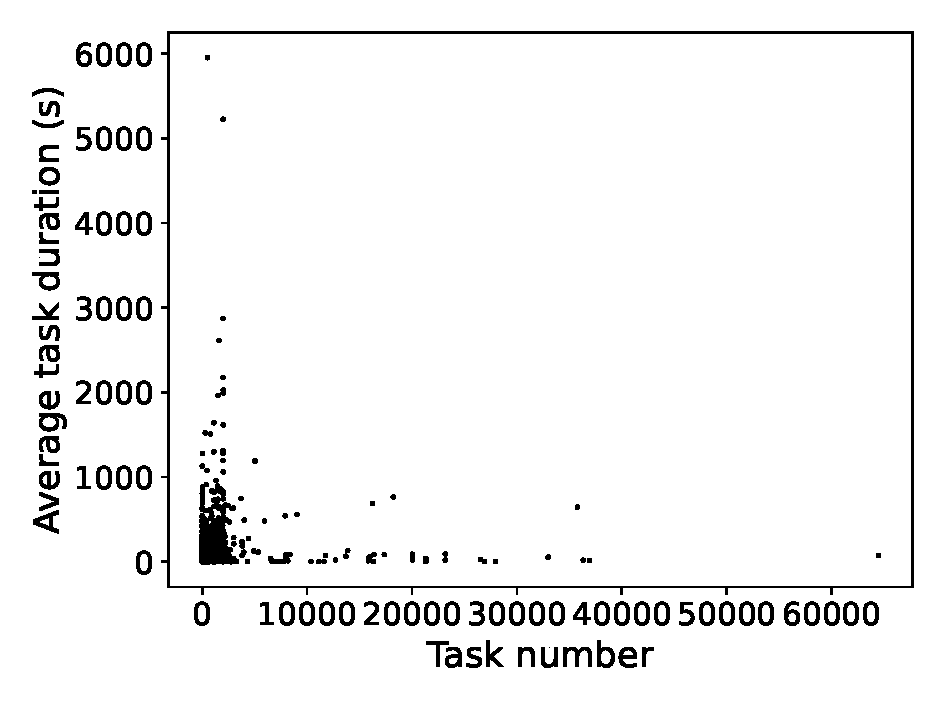
\includegraphics[width=0.47\linewidth]{Image2/JobDistribution_Ali20172D.eps}%
%\label{fig_second_case}
%\label{Fg:eg1}
}
\hfil
\subfloat[Alibaba 2018]
%
{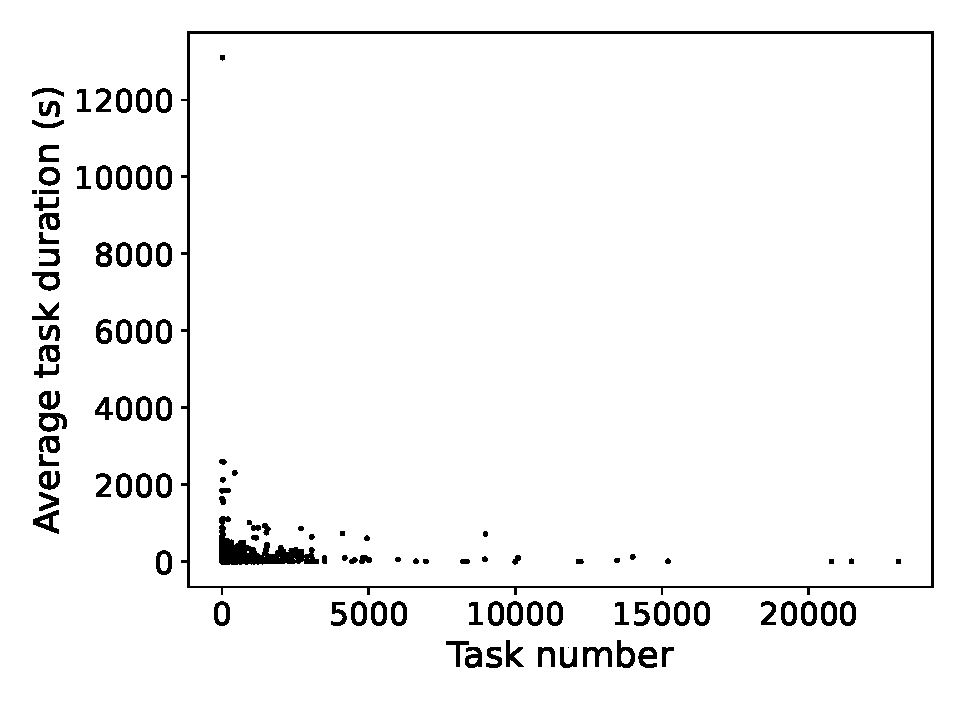
\includegraphics[width=0.48\linewidth]{Image2/JobDistribution_Ali2018_total2D.eps}%
%\label{Fg:eg2}
}
\caption{Job characteristic distribution of two datasets}
\label{fig:distribution2}
\end{figure}

We use cluster job traces sourced from the Alibaba Cluster Trace Program \cite{Ali2017}, which contains cluster traces of different years from real production. We pre-process the raw trace files of years 2017 and 2018, extract the key information including the arrival time, task number, average memory consumption and task processing times of each job. A continuous sequence of 10,000 jobs is randomly selected from each trace to serve as the dataset driving our simulations. The job characteristics of selected sequences are shown in Fig. \ref{fig:distribution} and Fig. \ref{fig:distribution_data}. 
Both sequences exhibit a heavy-tailed distribution, in which a small subset of jobs accounts for a disproportionately large share of the total computation load. We take the average memory consumption of each job as its data partition size. The average memory consumption records in the data traces are normalized values with respect to the memory capacity of the servers in the cluster. We derive the exact data partition size assuming that each server has 128GB RAM, under which the largest data partition is about 4GB. The average task number per job, average task processing time and average data partition size of all jobs are shown in Table \ref{tab:average_characteristic}.

%We use cluster job traces from Alibaba \cite{Ali2017} and Google \cite{Gg2019}. The Alibaba trace is sourced from the Alibaba Cluster Trace Program \cite{Ali2017}, and contains information on approximately 16 million tasks collected from 1300 machines over a period of 12 hours in August 2017. The Google trace is derived from the Borg cluster workload traces\cite{Gg2019}, containing around 30 GB compressed data of task events (e.g., a task is scheduled, completed or aborted) from Google's eight Borg cells over the month of May 2019. We pre-process both raw traces to extract key information, including the arrival time, task count, data partition size and task duration of each job. From each trace, a continuous sequence of 10,000 jobs is randomly selected to serve as the dataset driving our simulations. Characteristics of both datasets are shown in Fig. \ref{fig:distribution} and Fig. \ref{fig:distribution_data}. Both datasets exhibit a heavy-tailed distribution, in which a small subset of jobs accounts for a disproportionately large share of the total workload.  The data partition record in both data traces is a normalized value in homogeneous clusters; We derive the exact partition size with assumption that each cluster has 128GB RAM. The average task duration, average task count and average data partition size is shown in Table \ref{tab:average_characteristic}.


\begin{figure}[t]
\centering
\subfloat[Alibaba 2017]
{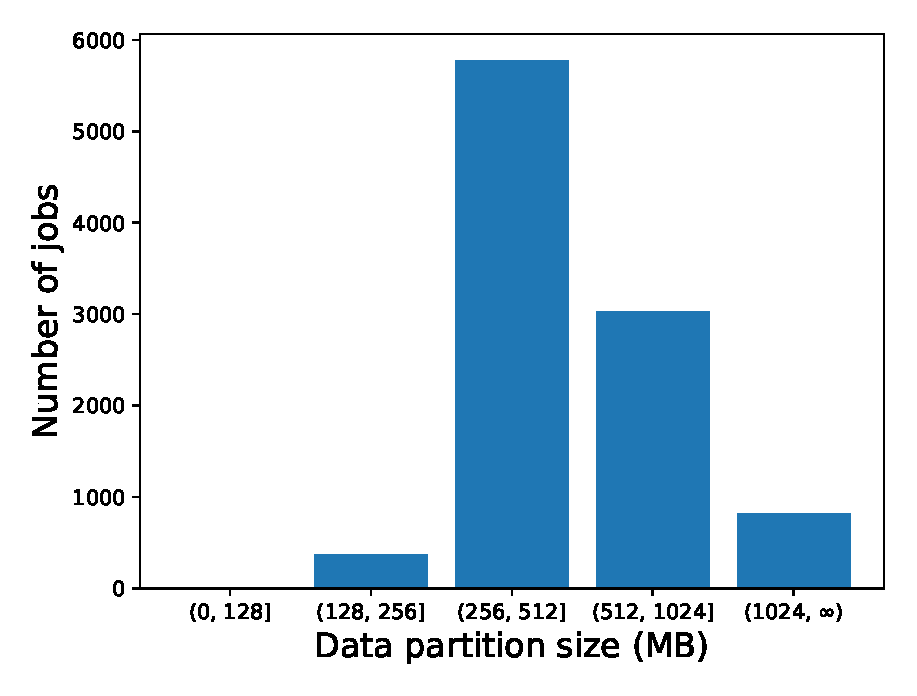
\includegraphics[width=0.455\linewidth]{Image2/data_Distribution_Ali2017.eps}%
%\label{fig_second_case}
%\label{Fg:eg1}
}
\hfil
\subfloat[Alibaba 2018]
%
{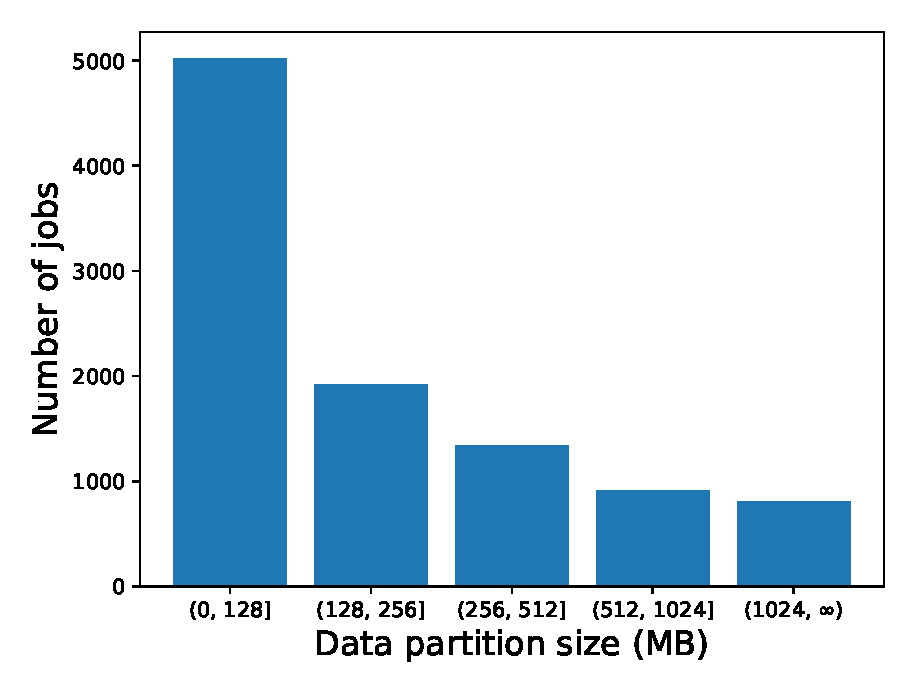
\includegraphics[width=0.455\linewidth]{Image2/data_Distribution_Ali2018_total.eps}%
%\label{Fg:eg2}
}
\caption{Data partition size distribution of two datasets}
\label{fig:distribution_data}
\end{figure}

\begin{table}[t]
\centering
\begin{tabular}{@{}lll@{}}
\hline
Characteristics & Alibaba 2017 & Alibaba 2018 \\
\hline
Average task number per job & $266.01$ & $94.70$ \\
\hline
Average task processing time (s) & $129.14$ & $82.41$ \\
\hline
Average data partition size (MB) & $661.15$ & $453.31$ \\
\hline
\end{tabular}
\caption{Job characteristics of two datasets}
\label{tab:average_characteristic}
\end{table}

\begin{figure*}[t]
\centering
\subfloat[utilization = 50\%]
{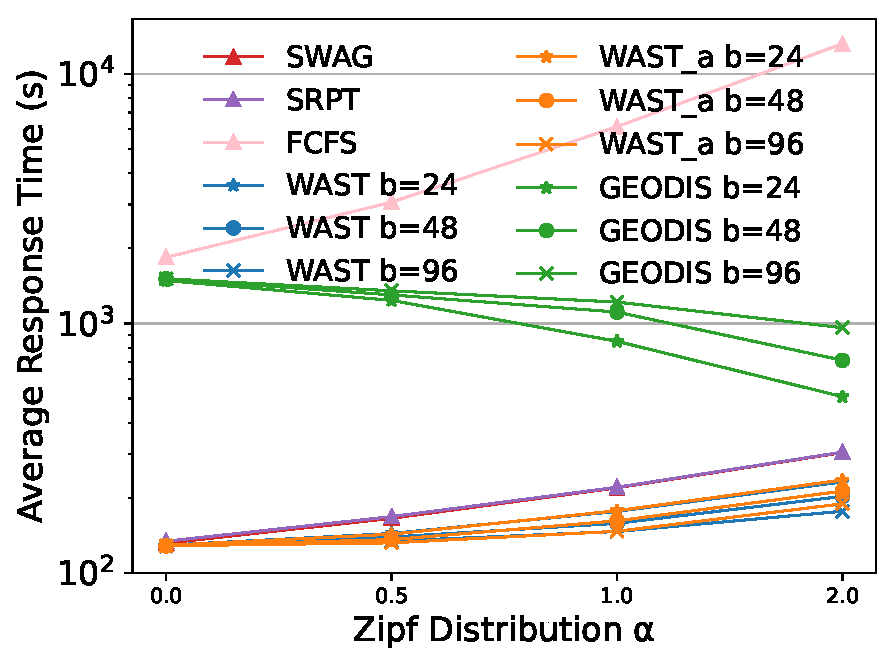
\includegraphics[width=0.24\textwidth]{Image2/Workload_Ali2018_4_50_GEODIS.eps}%
%\label{fig_second_case}
%\label{Fg:eg1}
}
\hfil
\subfloat[utilization = 60\%]
%
{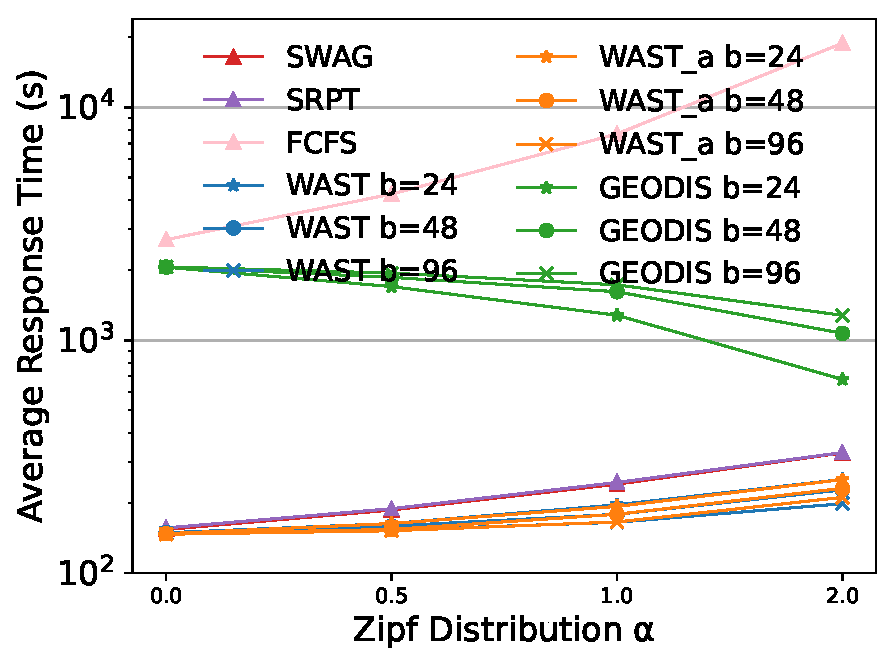
\includegraphics[width=0.24\textwidth]{Image2/Workload_Ali2018_4_60_GEODIS.eps}%
%\label{Fg:eg2}
}
\hfil
\subfloat[utilization = 70\%]
%
{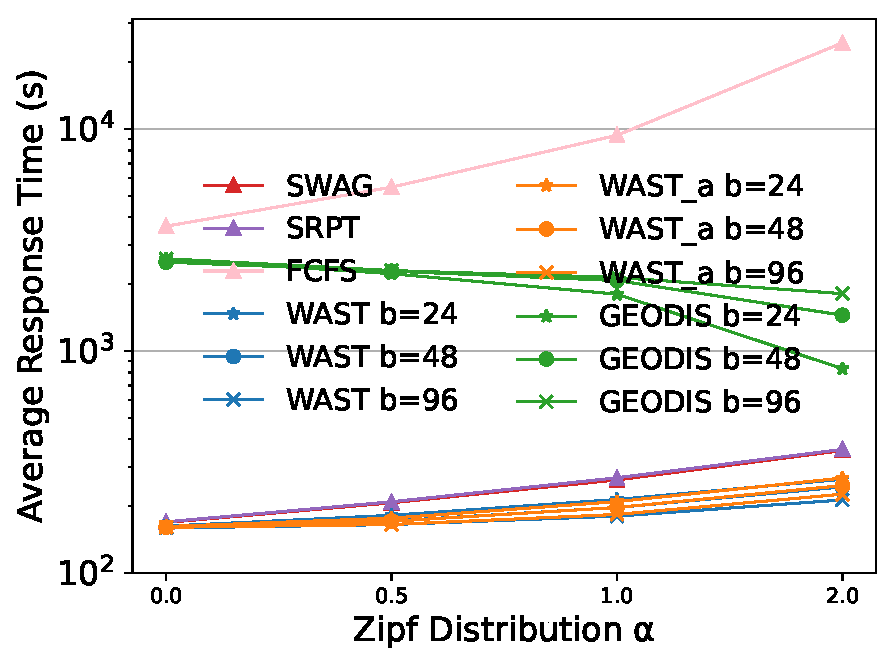
\includegraphics[width=0.24\textwidth]{Image2/Workload_Ali2018_4_70_GEODIS.eps}%
%\label{Fg:eg2}
}
\hfil
\subfloat[utilization = 80\%]
%
{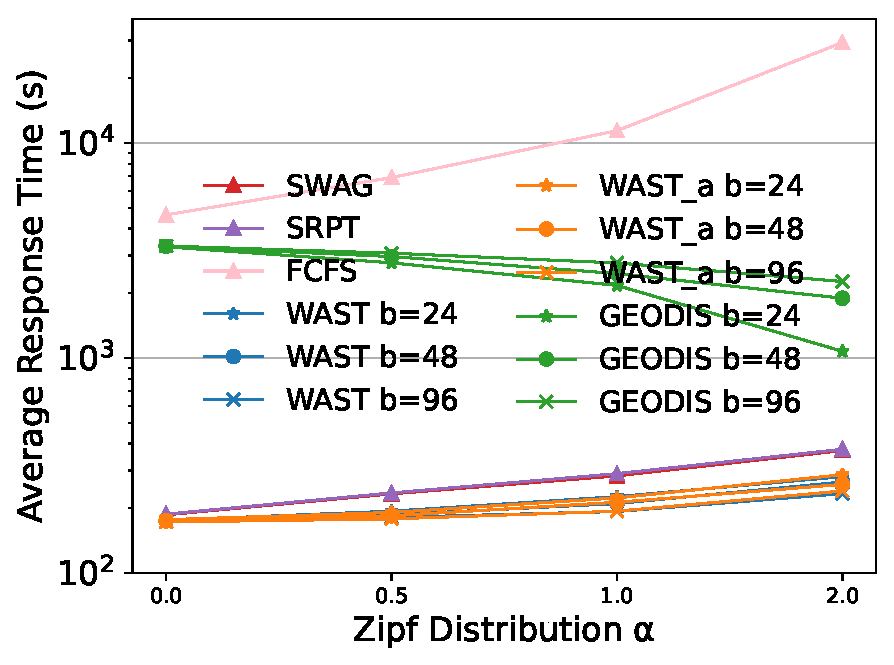
\includegraphics[width=0.24\textwidth]{Image2/Workload_Ali2018_4_80_GEODIS.eps}%
%\label{Fg:eg2}
}
\caption{Average Job Response Time Compared with GEODIS, Alibaba 2018}
\label{fig:JRT_GEODIS}
\end{figure*}

\begin{figure*}[t]
\centering
\subfloat[utilization = 50\%]
{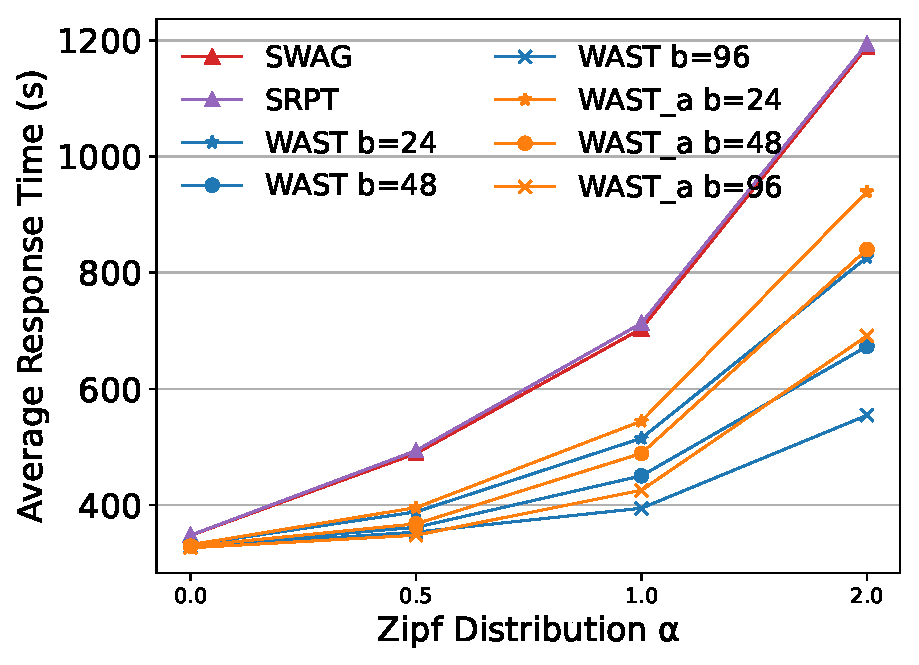
\includegraphics[width=0.24\textwidth]{Image2/Workload_Ali2017_50.eps}%
%\label{fig_second_case}
%\label{Fg:eg1}
}
\hfil
\subfloat[utilization = 60\%]
%
{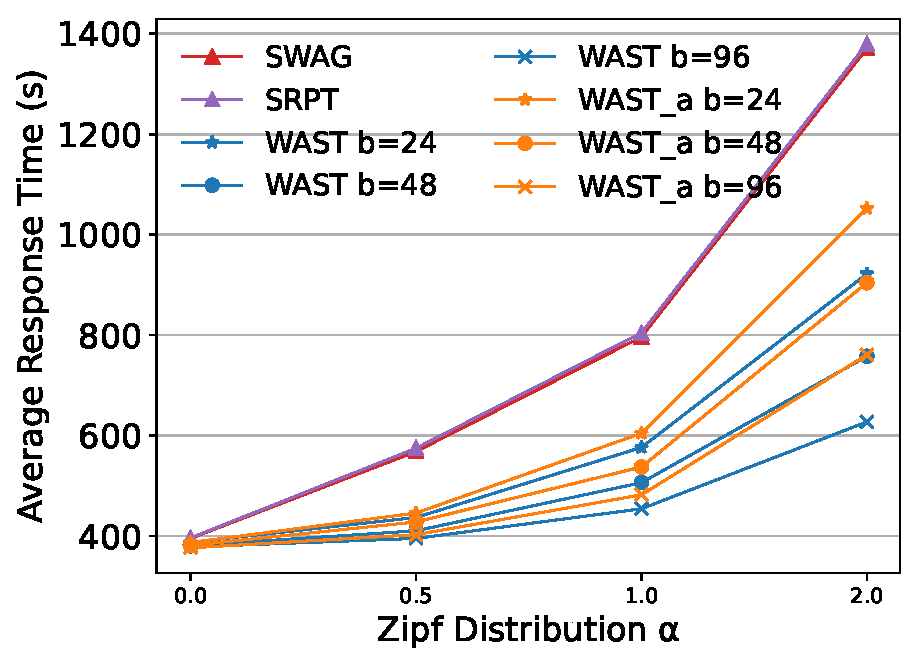
\includegraphics[width=0.24\textwidth]{Image2/Workload_Ali2017_60.eps}%
%\label{Fg:eg2}
}
\hfil
\subfloat[utilization = 70\%]
%
{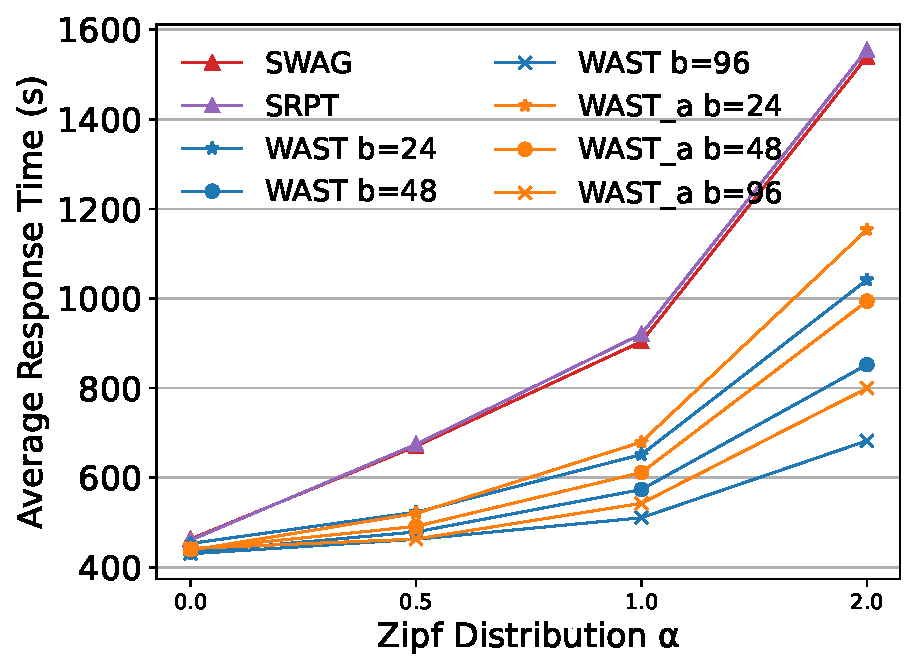
\includegraphics[width=0.24\textwidth]{Image2/Workload_Ali2017_70.eps}%
%\label{Fg:eg2}
}
\hfil
\subfloat[utilization = 80\%]
%
{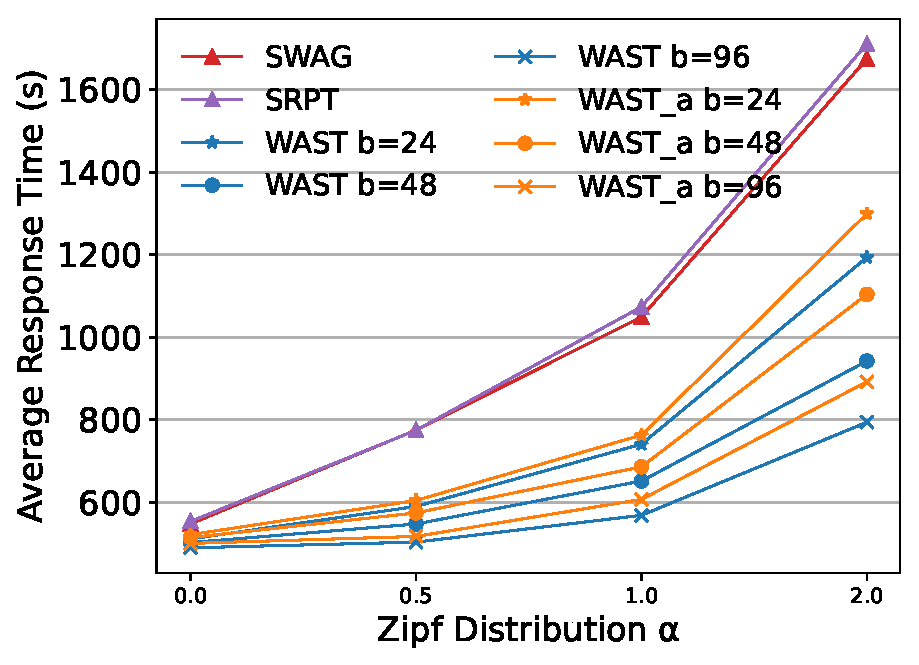
\includegraphics[width=0.24\textwidth]{Image2/Workload_Ali2017_80.eps}%
%\label{Fg:eg2}
}
\caption{Average Job Response Time, Alibaba 2017}
\label{fig:JRT}
\end{figure*}

\begin{figure*}[t]
\centering
\subfloat[utilization = 50\%]
{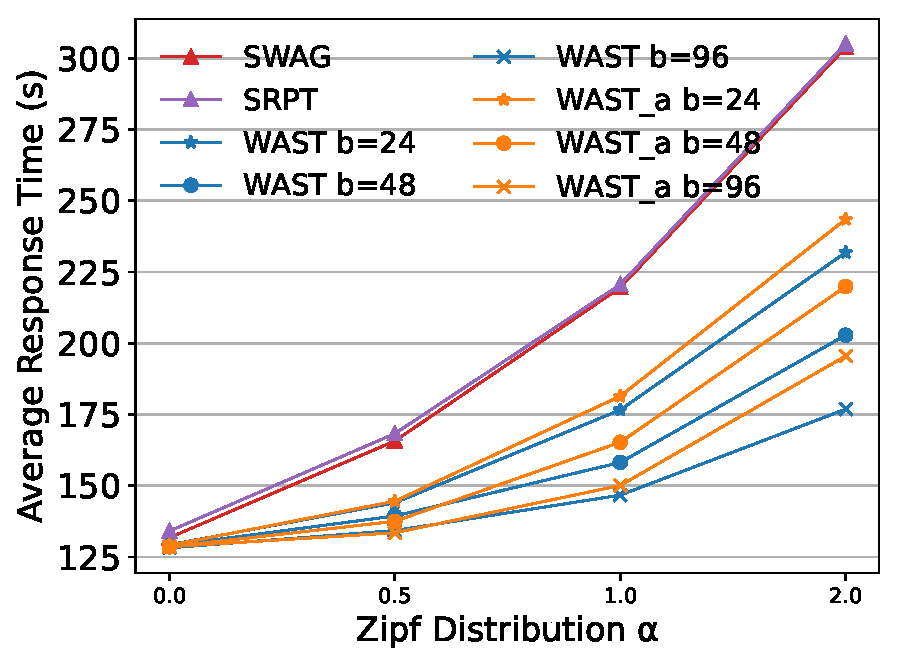
\includegraphics[width=0.24\textwidth]{Image2/Workload_Ali2018_4_50.eps}%
%\label{fig_second_case}
%\label{Fg:eg1}
}
\hfil
\subfloat[utilization = 60\%]
%
{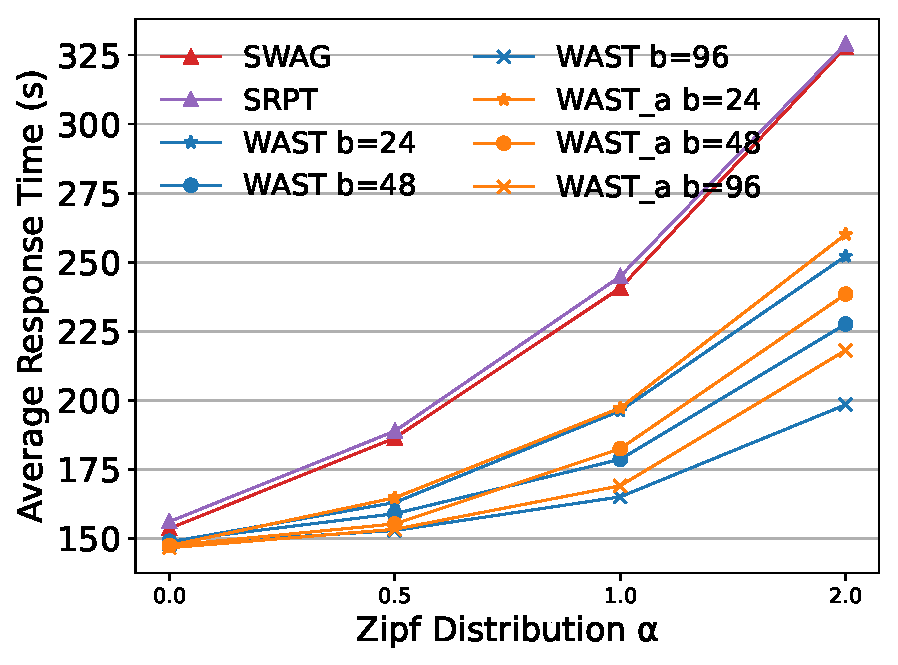
\includegraphics[width=0.24\textwidth]{Image2/Workload_Ali2018_4_60.eps}%
%\label{Fg:eg2}
}
\hfil
\subfloat[utilization = 70\%]
%
{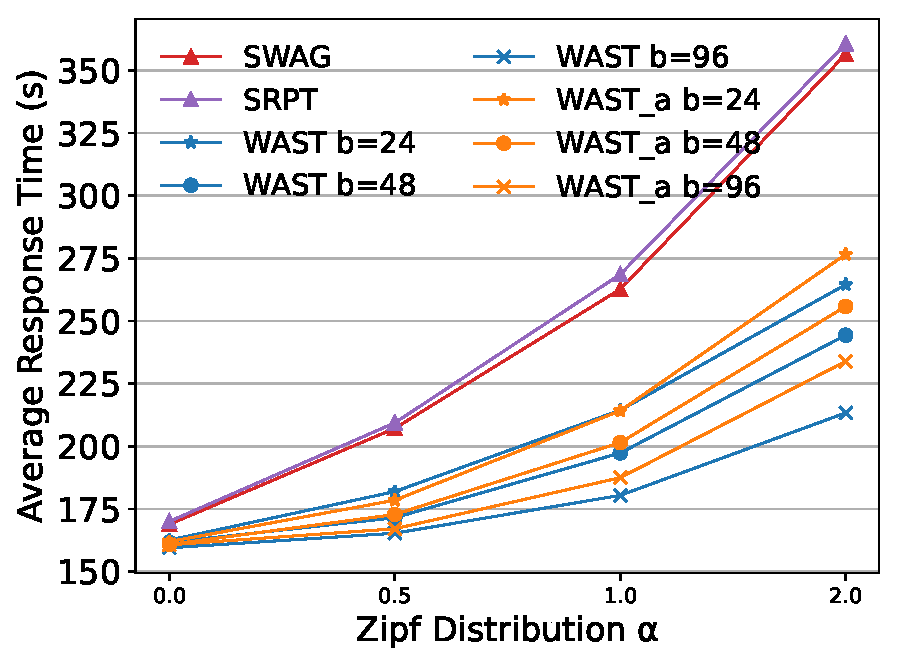
\includegraphics[width=0.24\textwidth]{Image2/Workload_Ali2018_4_70.eps}%
%\label{Fg:eg2}
}
\hfil
\subfloat[utilization = 80\%]
%
{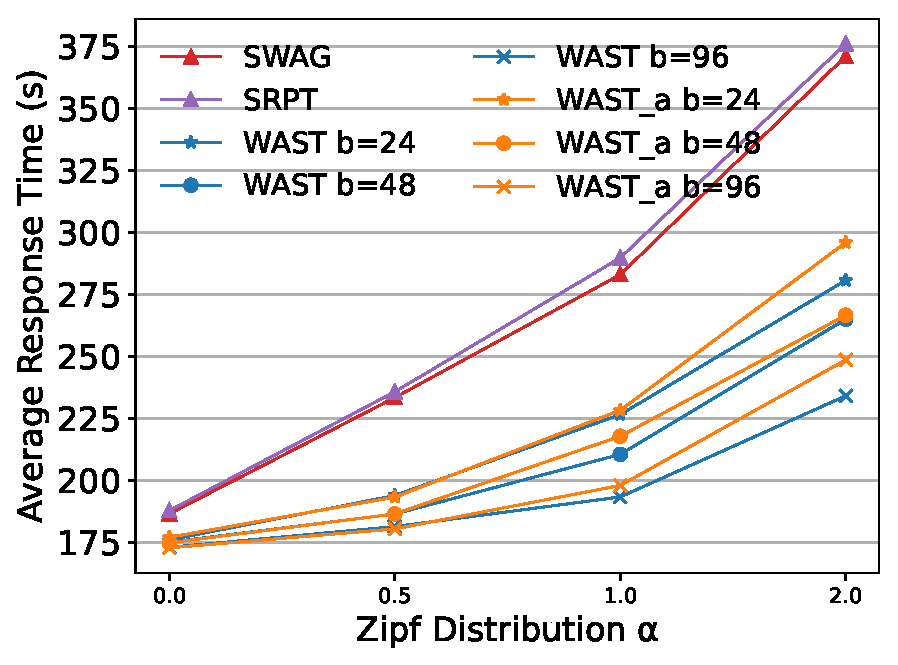
\includegraphics[width=0.24\textwidth]{Image2/Workload_Ali2018_4_80.eps}%
%\label{Fg:eg2}
}
\caption{Average Job Response Time, Alibaba 2018}
\label{fig:JRT2}
\end{figure*}


\subsection{System Configuration}
We simulate a distributed system of $m$ sites, each with the same number of computing slots. Each task is assumed to take up one computing slot to run and release it after completion. Due to the switching overhead consideration, we assume that the system does not allow preemption during task execution. For each job, the initial distribution of its tasks among the sites is generated by a Zipf distribution: the numbers of tasks placed at the $m$ sites are proportional to $1, \frac{1}{2^\alpha}, \frac{1}{3^\alpha}, ..., \frac{1}{m^\alpha}$, where $\alpha$ is a Zipf parameter. A higher $\alpha$ implies a more skewed distribution (a higher proportion of tasks are concentrated at fewer sites), whereas $\alpha$ = $0$ indicates a uniform distribution. In the experiments, we test four Zipf distributions with $\alpha$ set to $0$, $0.5$, $1$ and $2$ to simulate different task distributions of jobs. After the task distribution is generated, we shuffle the order of the sites when deploying each job's task distribution, so that the total workload at each site 
%(i.e., the total execution time of the tasks of all jobs deployed at each site) 
is roughly balanced. 
We scale the arrival times of the jobs in the datasets to simulate different levels of overall system utilization. We assume that the system is fully connected, i.e., a direct link exists between any two sites. The available bandwidth is set to $24$Mbps, $48$Mbps or $96$Mbps for all links. We experiment with different numbers of sites, different numbers of computing slots per site, and different levels of system utilization. The results show similar performance trends. Due to space limitations, we focus on presenting the results for $m=10$ sites, 32 computing slots per site, and system utilization = $50\%$, $60\%$, $70\%$ and $80\%$.  
%\sout{and a system workload of 60\%}
%As mentioned in Section \ref{sec:dataset}, the average data partition size of the Alibaba and Google data trace is a normalized value; We suppose that 

\subsection{Scheduling Policies}
In Section \ref{sec:WAST}, we have introduced the WAST algorithm and its fast approximation WAST\_a. For comparison, we also simulate the following baseline algorithms.
\begin{itemize}
    \item \textbf{First-Come-First-Serve (FCFS)}: FCFS simply schedules jobs in the order of their arrival times. When a computing slot becomes available, it is assigned to the job that arrives the earliest and has pending tasks.
    
    \item \textbf{Shortest Remaining Processing Time (SRPT)}: SRPT schedules jobs based on their estimated completion times in the case that each job runs alone in the system. More specifically, it estimates the completion time of a job $J_k$ as $\max_{j \in[m]} \lceil d_{kj}/u_j\rceil \cdot l_k$, and executes pending jobs based on this estimation from low to high.% The original SRPT assumes that each site has one computation slot only (i.e., the estimated completion time of each job $J_k$ is equal to the $\max_{j \in[m]} (l_k*d_{kj})$), and we adapt it to the case that each site has multiple slots. %In other words, SRPT places each job's distributed workload to the empty system and computes its job response time, and the job execution order is derived based on these estimated job response times.

    \item \textbf{Workload-Aware Greedy Scheduling (SWAG)} \cite{hung2015scheduling}: SWAG greedily schedules jobs iteratively by estimating their completion times based on scheduled workloads without using network resources to transfer tasks between sites. %It iteratively selects the job with the lowest completion time and add the job's computation loads to the system. 
    Our WAST algorithm degenerates to SWAG when network resources are not available in the system. %In each round, given the computation load of scheduled jobs of previous rounds, SWAG traverses each unscheduled job and computes its estimated completion time by assigning its task to the corresponding sites%SWAG is also designed for the single-slot case and it does not consider utilizing the network resource within the system. We modify SWAG to support the case where each site has multiple computation slots.

    \item \textbf{GEODIS} \cite{GEODIS}: GEODIS models job scheduling in geo-distributed data centers as a joint optimization of task placement and data access. It employs a heuristic scheduling algorithm which is triggered when any data center completes its scheduled workload. The objective of scheduling is to minimize the makespan of job execution (the latest job completion time) by selectively migrating data over faster network links when local servers are overloaded.
\end{itemize}
%
%The improvement becomes more pronounced when jobs' workload distribution is more skewed among sites and when higher bandwidth is available, since the utilization of network resource has greater potential in mitigating the workload imbalances of each job under these conditions. Furthermore, the algorithm performs better on the Alibaba 2017 data trace
In the experiments, we use OR-Tools \cite{ortools} to solve the minimum-cost flow problems in WAST. All algorithms (except FCFS) take the average task processing time of each job as input for scheduling and assume that the processing times of all tasks of the job are equal to the average. The simulation, on the other hand, uses the real processing times of individual tasks recorded in the trace to derive the job response time.

\subsection{Experimental Results}
Fig. \ref{fig:JRT_GEODIS} shows the performance of all algorithms in terms of average job response time. Due to space limitations, we only present the results for the Alibaba 2018 dataset 
%under system utilization of $60\%$ and $80\%$ 
(the results for the Alibaba 2017 dataset are similar). Note that the y-axis is plotted on a logarithmic scale. The results indicate that the average job response times of FCFS and GEODIS are one to two orders of magnitude higher than the other algorithms. This is because FCFS does not optimize job execution order and GEODIS is primarily designed to minimize the makespan.

Figs. \ref{fig:JRT} and \ref{fig:JRT2} zoom into the performance of the remaining algorithms for both datasets. %The results of the FCFS strategy are more than two orders of magnitude higher than those of the other algorithms and hence are not included in the figures. 
Compared to SRPT and SWAG, the average job response time of WAST and WAST\_a is reduced by up to $53.3\%$ for the Alibaba 2017 trace and $42.1\%$ for the Alibaba 2018 trace. The improvement becomes more pronounced when the task distribution of jobs across sites is more skewed and when higher bandwidth is available, as more network resources can be effectively utilized to mitigate the imbalance in the task distribution of jobs under these conditions. Moreover, our WAST algorithm performs better for the Alibaba 2017 trace than the Alibaba 2018 trace. This is because the higher average task number per job in Alibaba 2017 leads to more tasks accumulated at some particular sites under highly uneven task distributions, resulting in increased response times if task transmission is not conducted. This, in turn, allows the WAST algorithm to offload more tasks from peak-load sites, enhancing the advantage of WAST. 
In addition, Figs. \ref{fig:JRT} and \ref{fig:JRT2} show that although WAST\_a compromises the quality of scheduling and performs slightly worse than WAST, it still significantly outperforms the baseline algorithms.%demonstrating that it is an effective approximation to WAST.%the ratio of average task duration to average data partition size is higher in 2017. This allows a greater number of tasks to be transmitted within the average task execution time, thereby providing additional opportunities to reduce job response time through task migration. Furthermore, 

% \begin{figure}[t]
% \centering
% \subfloat[utilization=60\%]
% {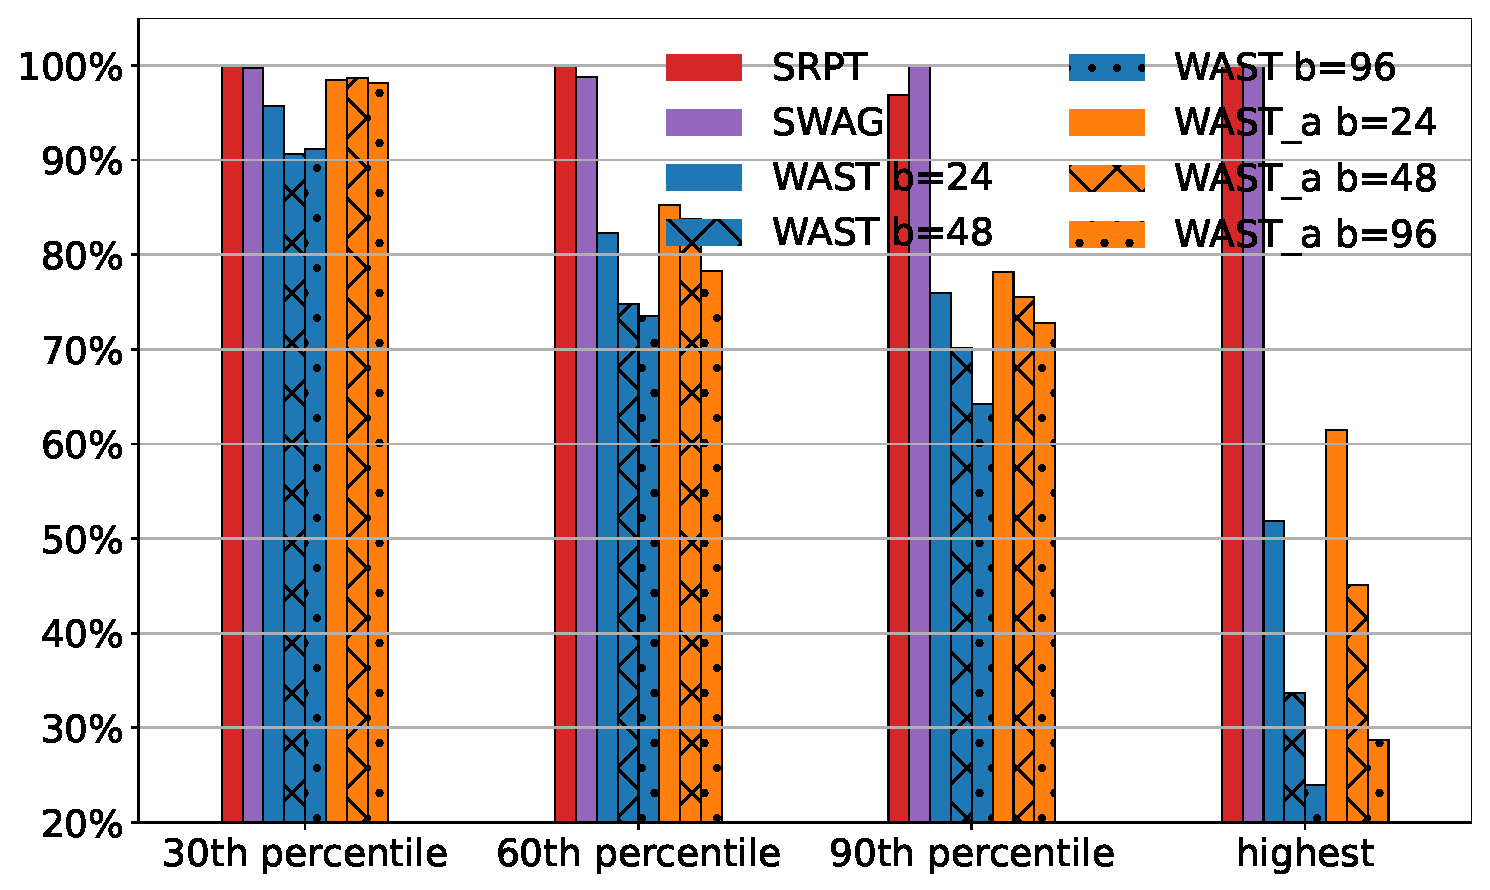
\includegraphics[width=0.48\linewidth]{Image2/CDFpercentile_Ali2017_60.eps}%
% %\label{fig_second_case}
% %\label{Fg:eg1}
% }
% \hfil
% \subfloat[utilization=80\%]
% %
% {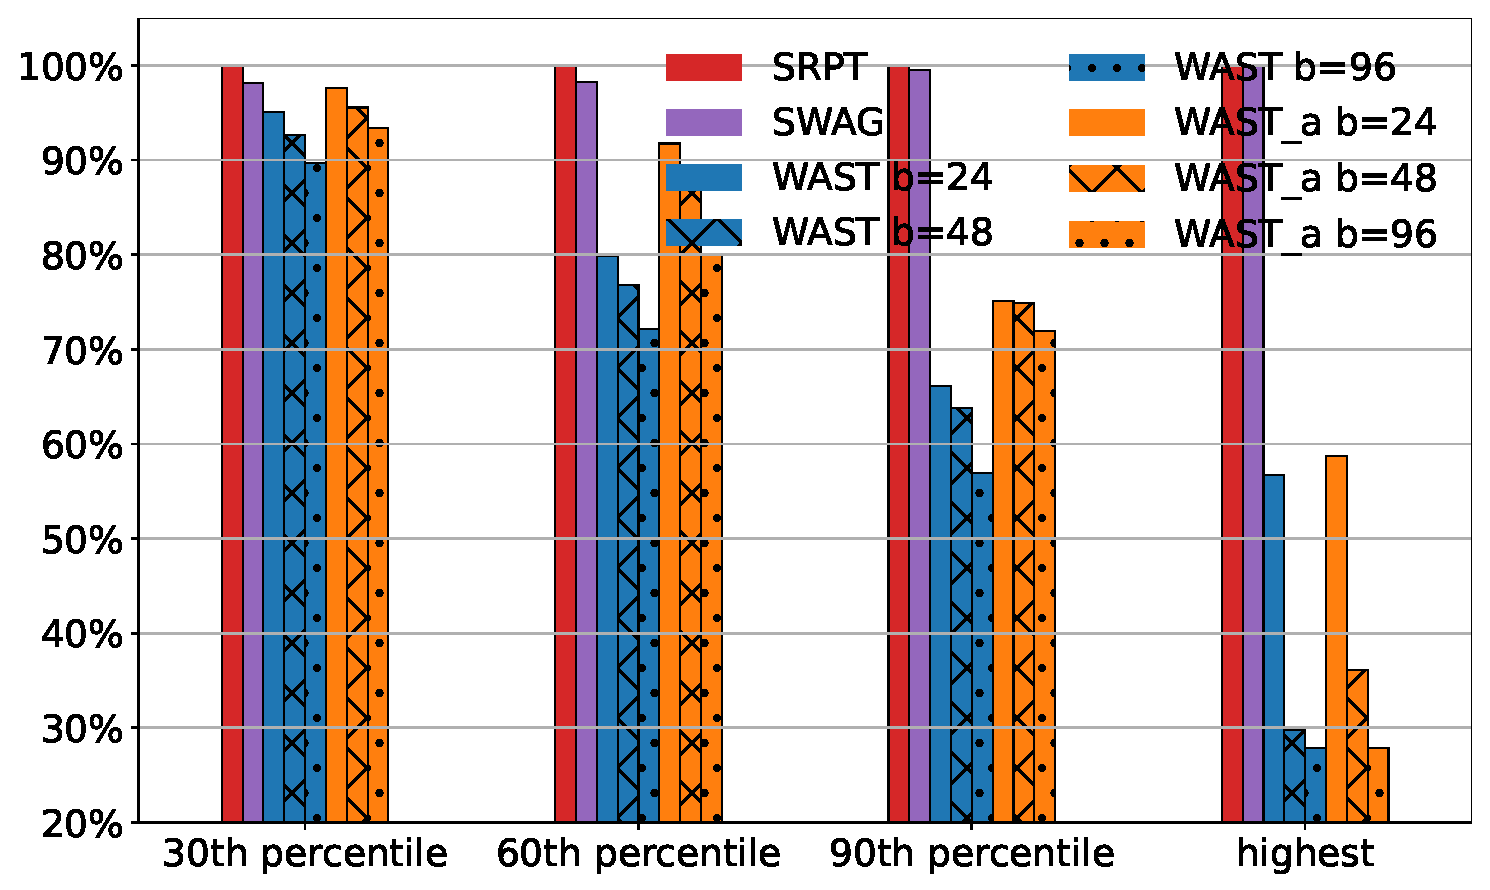
\includegraphics[width=0.48\linewidth]{Image2/CDFpercentile_Ali2017_80.eps}%
% %\label{Fg:eg2}
% }
% \caption{Response Time at Different Percentiles, Alibaba 2017, $\alpha=1$}
% \label{fig:JRT_CDF_2017}
% \end{figure}

% \begin{figure}[t]
% \centering
% \subfloat[utilization=60\%]
% {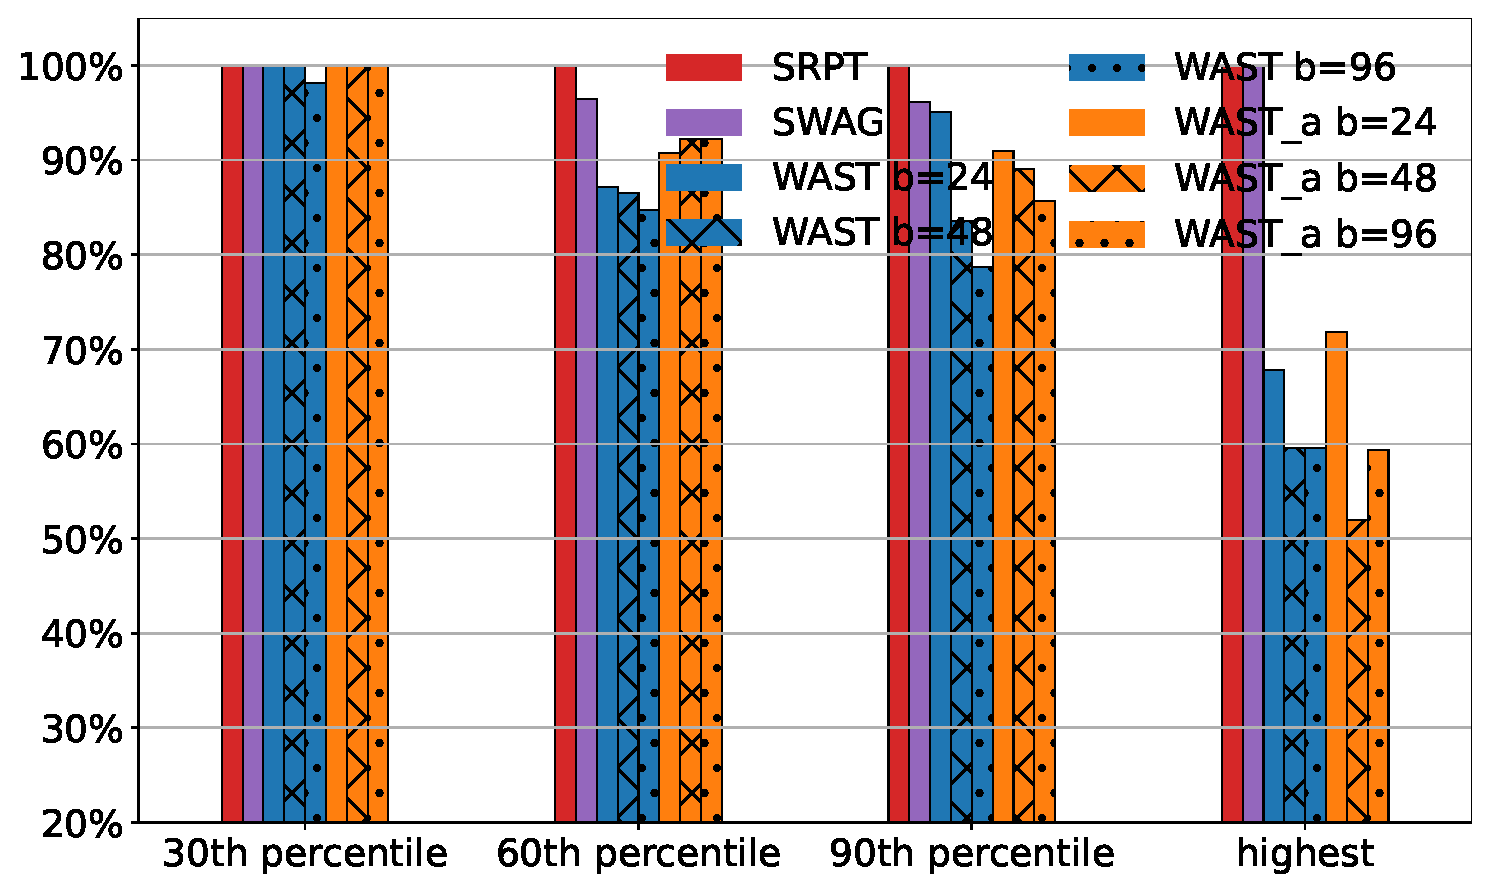
\includegraphics[width=0.48\linewidth]{Image2/CDFpercentile_Ali2018_4_60.eps}%
% %\label{fig_second_case}
% %\label{Fg:eg1}
% }
% \hfil
% \subfloat[utilization=80\%]
% %
% {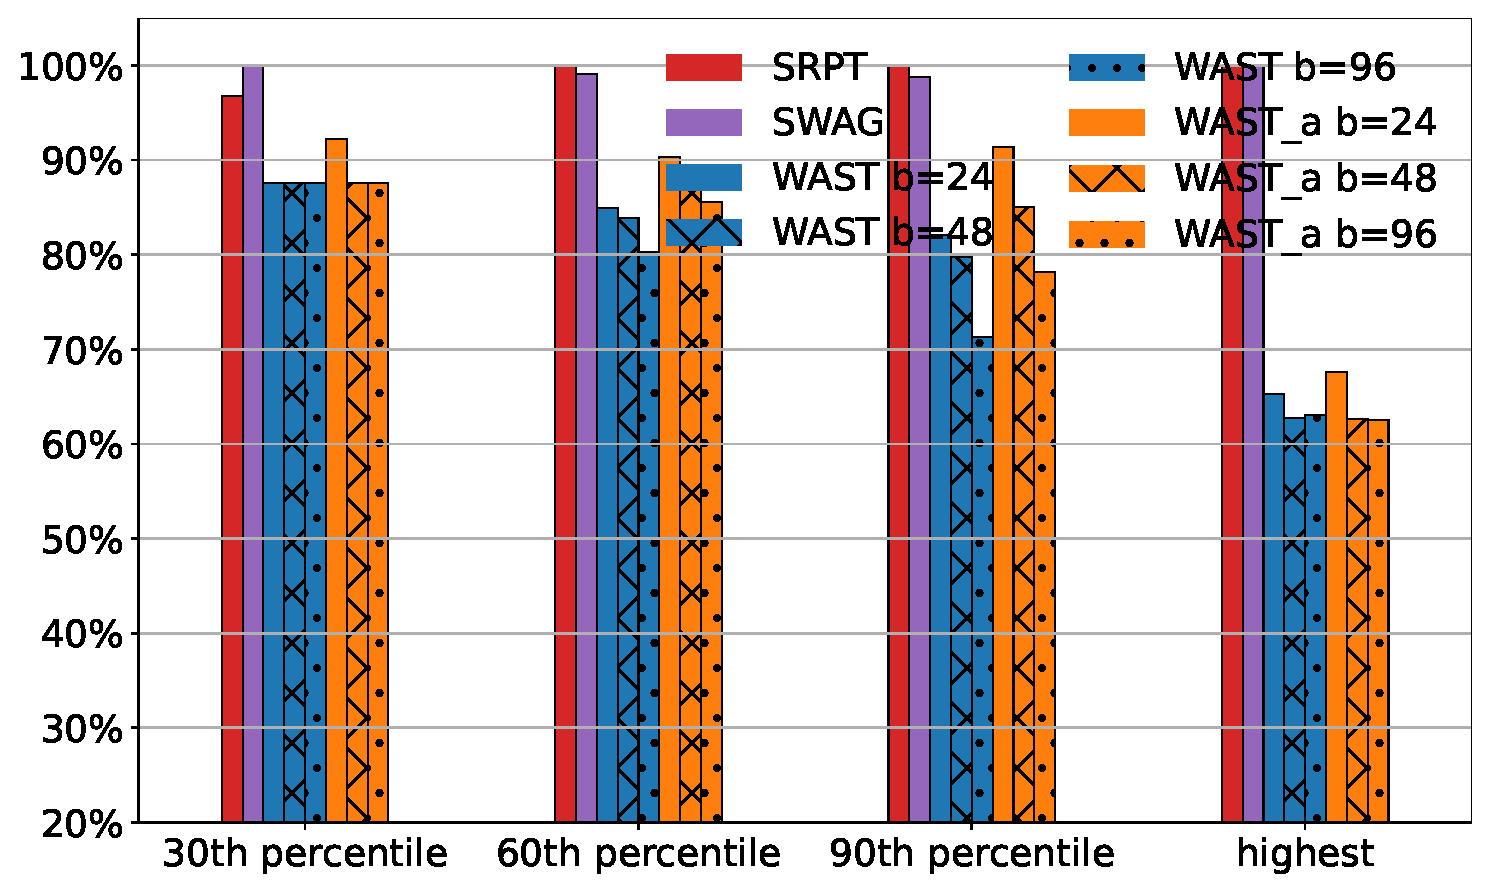
\includegraphics[width=0.48\linewidth]{Image2/CDFpercentile_Ali2018_4_80.eps}%
% %\label{Fg:eg2}
% }
% \caption{Response Time at Different Percentiles, Alibaba 2018, $\alpha=1$}
% \label{fig:JRT_CDF_2018}
% \end{figure}
Figs. \ref{fig:JRT_CDF} and \ref{fig:JRT_CDF2} show the $30$th, $60$th, $90$th percentiles and the highest job response times for both datasets, under the Zipf distribution with $\alpha=1$. For each percentile, the longest job response time among algorithms is normalized to 1, and the job response times of other algorithms are expressed relative to it. It can be seen that jobs in the lower percentiles have little improvement when the WAST and WAST\_a algorithms are applied, since these jobs are small and have already achieved nearly best response times under the SRPT and SWAG strategies which favor small jobs. On the other hand, WAST and WAST\_a can significantly enhance the performance of large jobs whose response times are relatively longer by transferring their tasks to mitigate their imbalanced task distributions. The highest job response time can be improved by more than $70\%$, as shown in Fig. \ref{fig:JRT_CDF}.

\begin{figure*}[t]
\centering
\subfloat[utilization = 50\%]
{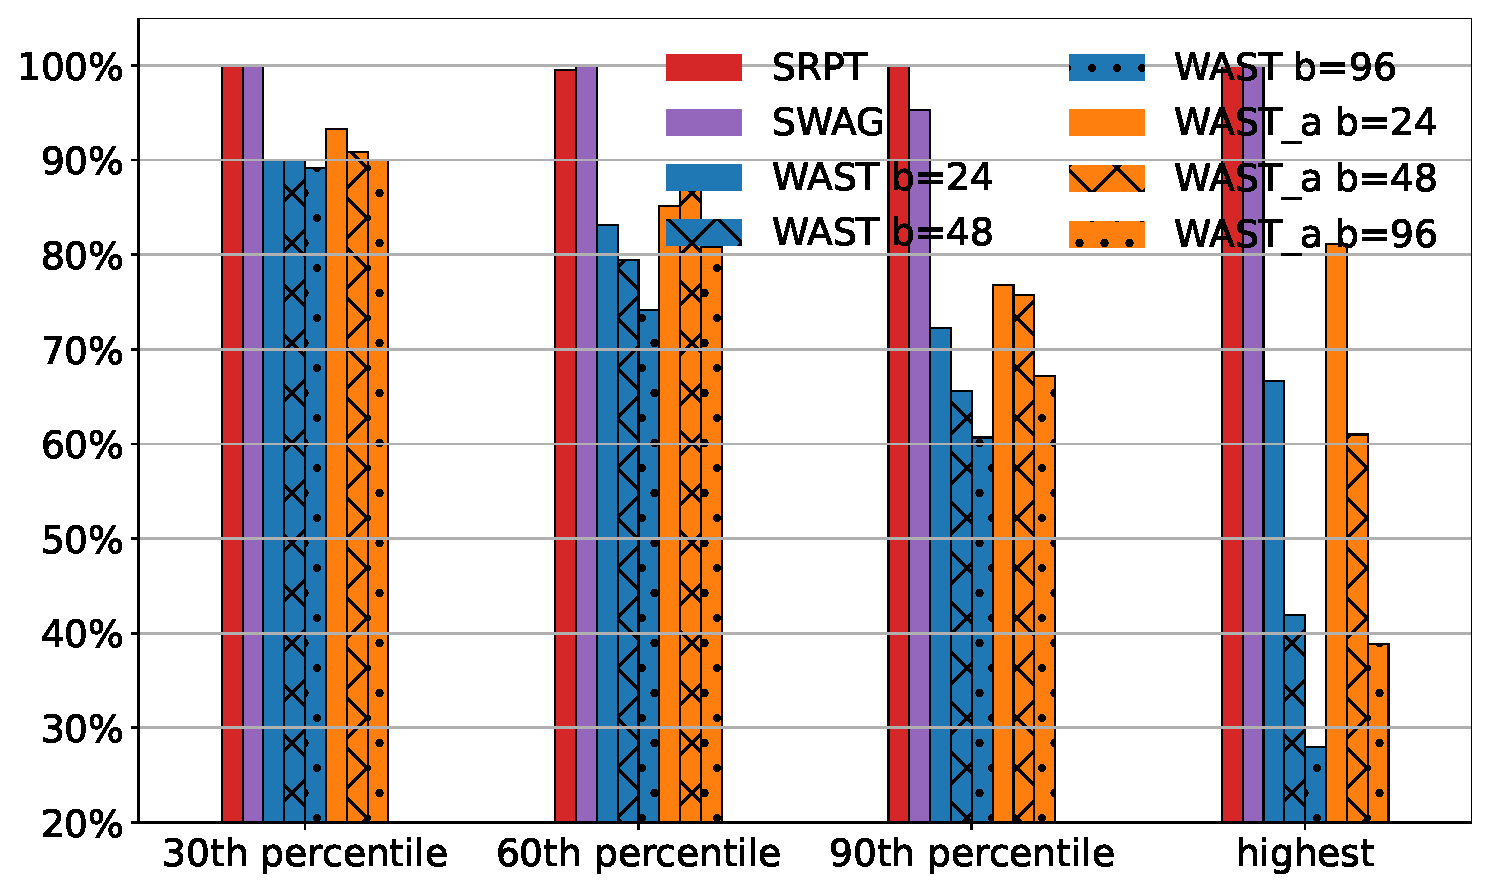
\includegraphics[width=0.24\textwidth]{Image2/CDFpercentile_Ali2017_50.eps}%
\label{fig:JRT_CDF_a}
}
\hfil
\subfloat[utilization = 60\%]
%
{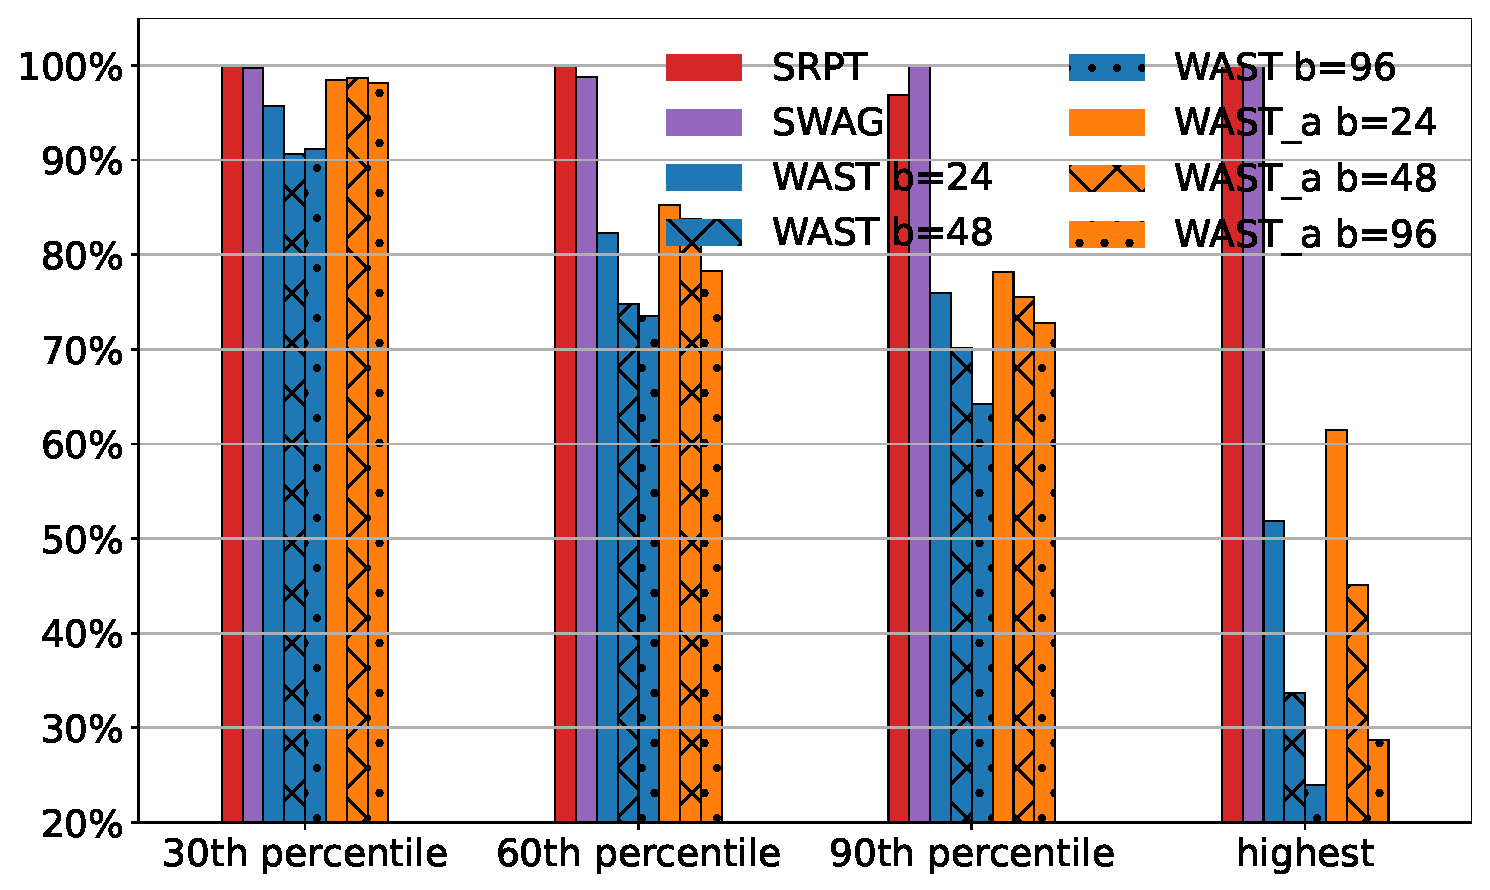
\includegraphics[width=0.24\textwidth]{Image2/CDFpercentile_Ali2017_60.eps}
\label{fig:JRT_CDF_b}
}%
\hfil
\subfloat[utilization = 70\%]
%
{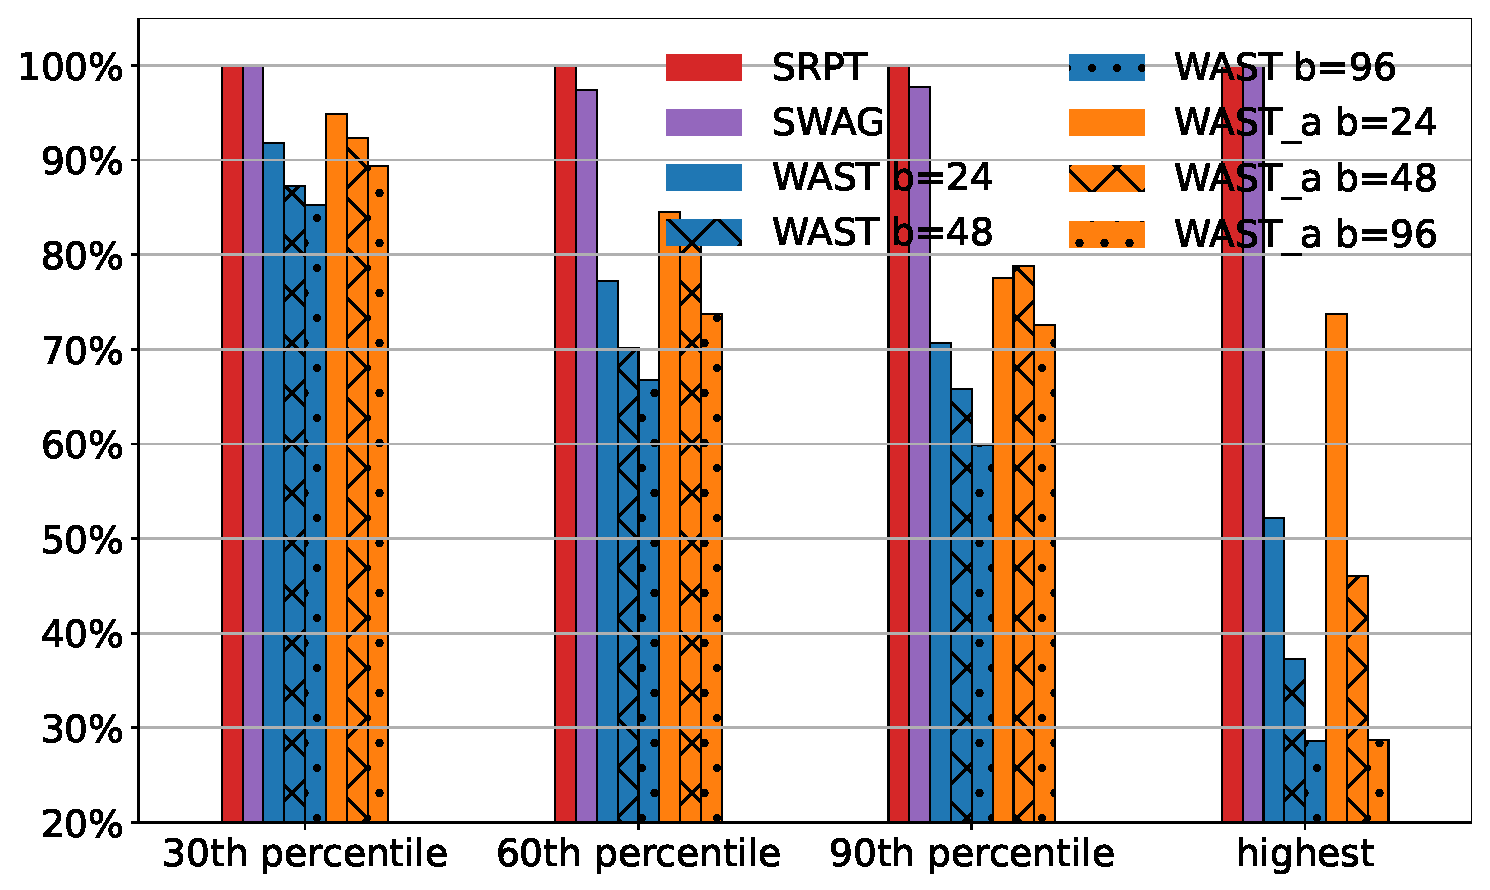
\includegraphics[width=0.24\textwidth]{Image2/CDFpercentile_Ali2017_70.eps}}%
\hfil
\subfloat[utilization = 80\%]
%
{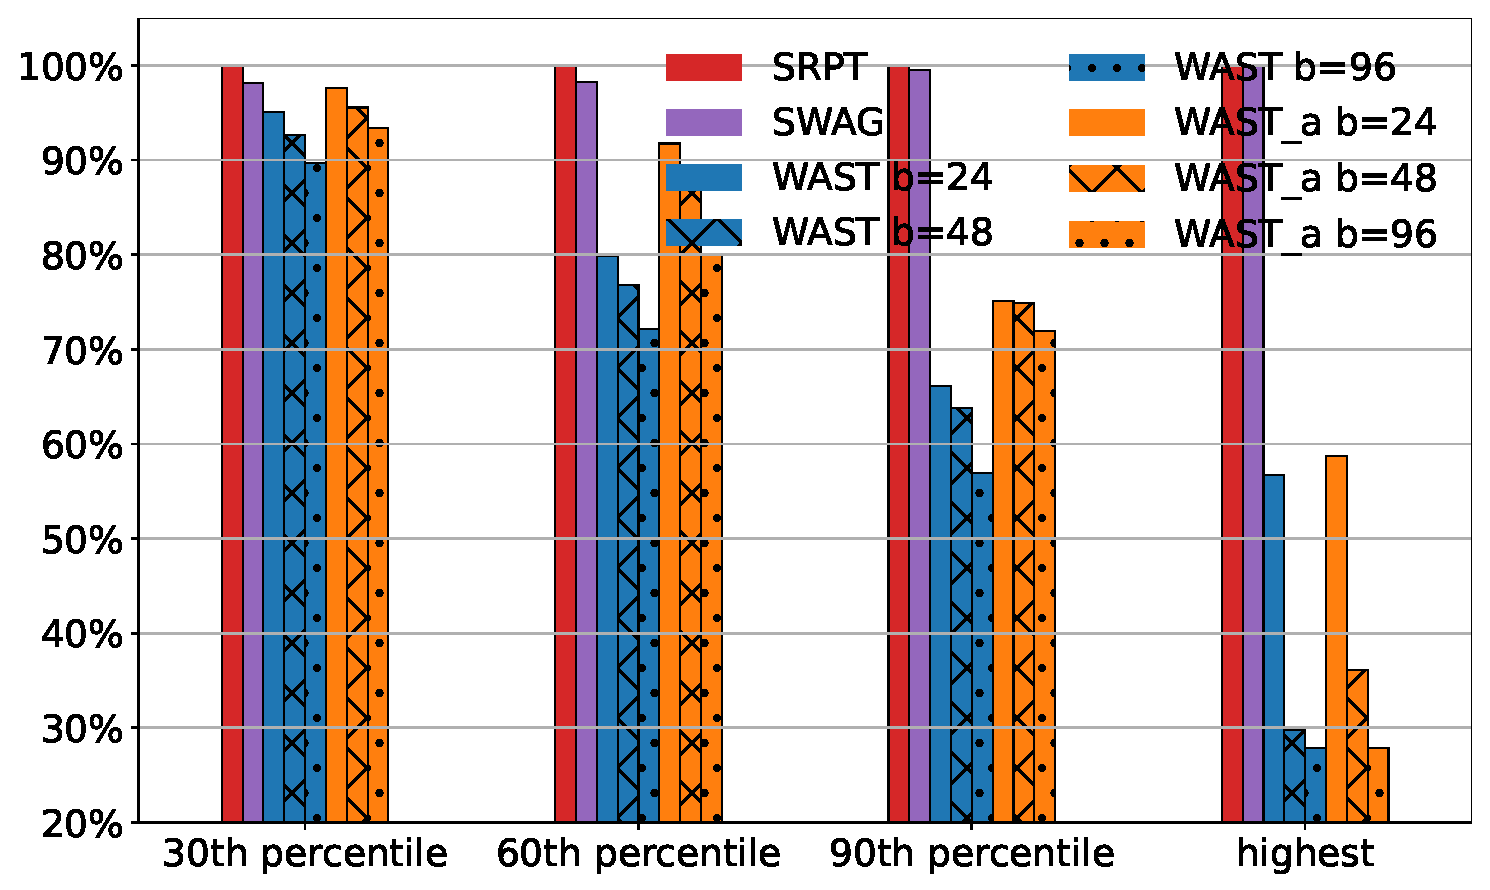
\includegraphics[width=0.24\textwidth]{Image2/CDFpercentile_Ali2017_80.eps}
%\label{Fg:eg2}
}
\caption{Job Response Time at Different Percentiles, Zipf Distribution $\alpha=1$, Alibaba 2017}
\label{fig:JRT_CDF}
\end{figure*}

\begin{figure*}[t]
\centering
\subfloat[utilization = 50\%]
{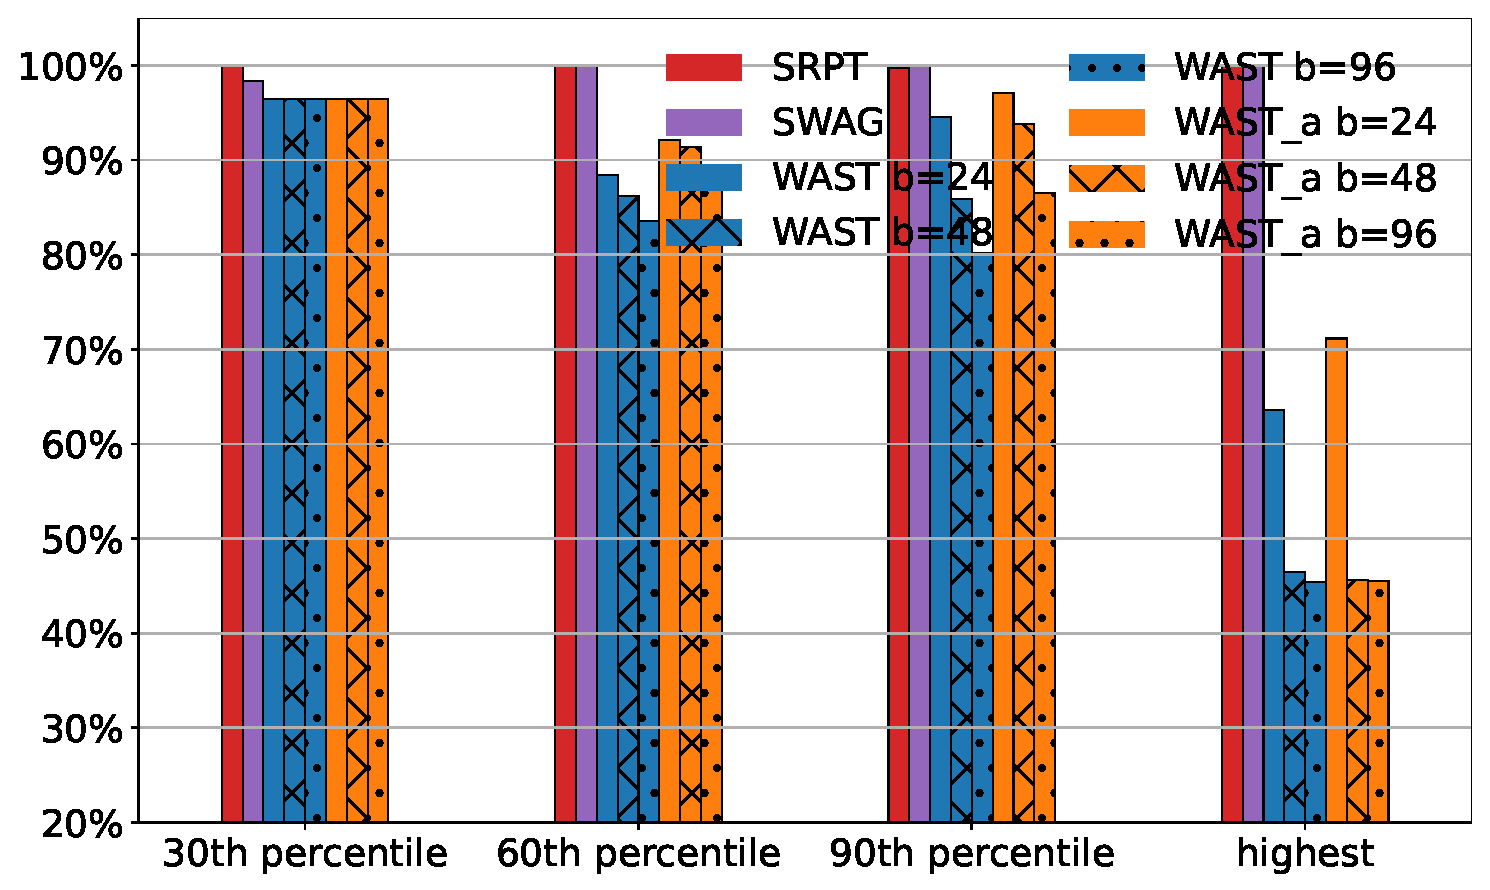
\includegraphics[width=0.24\textwidth]{Image2/CDFpercentile_Ali2018_4_50.eps}%
\label{fig:JRT_CDF_a}
}
\hfil
\subfloat[utilization = 60\%]
%
{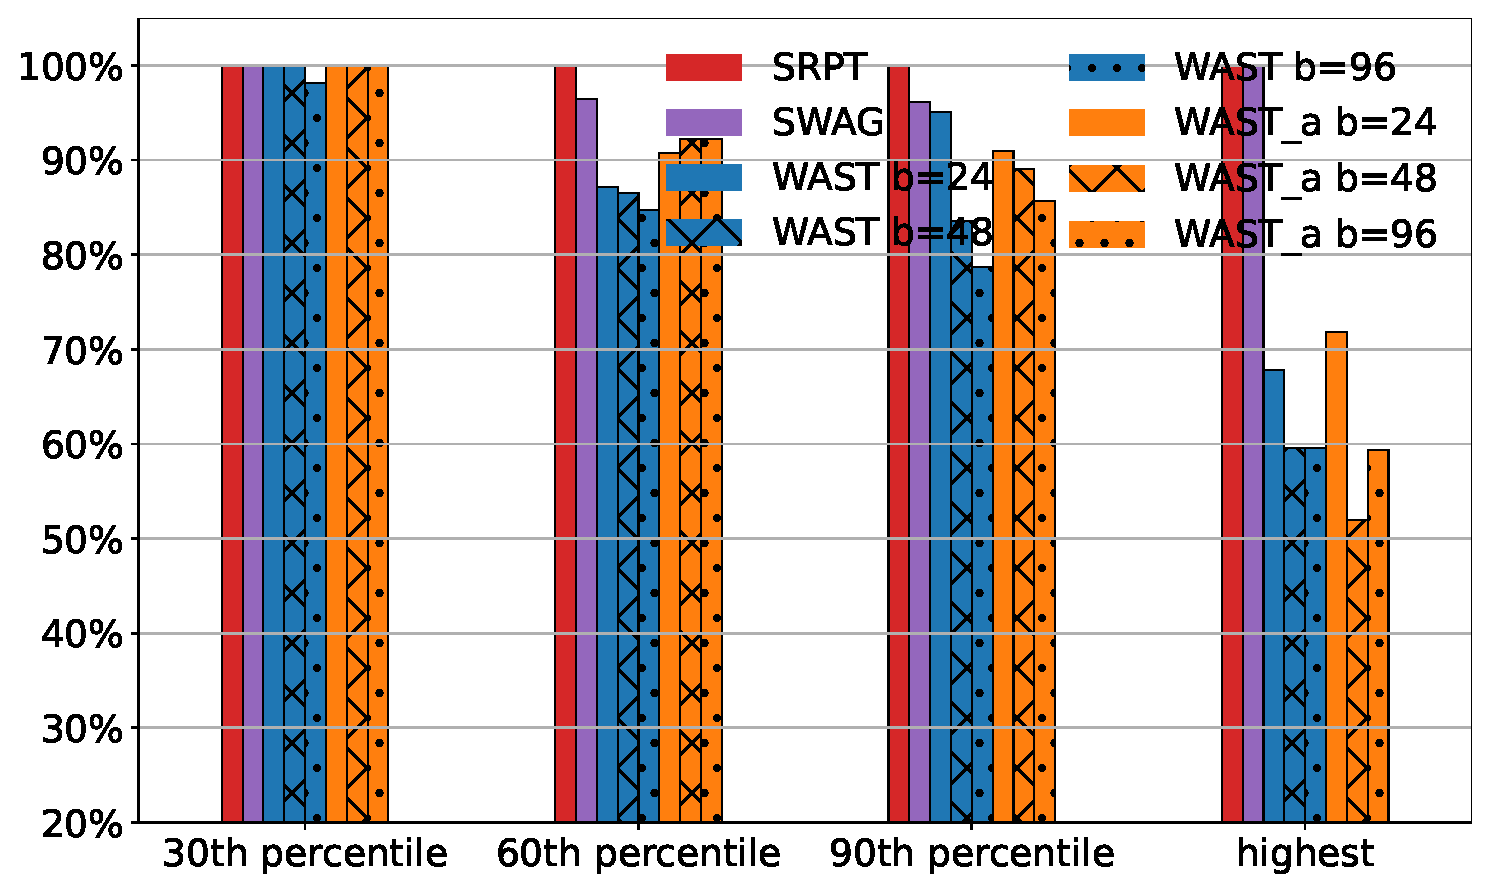
\includegraphics[width=0.24\textwidth]{Image2/CDFpercentile_Ali2018_4_60.eps}
\label{fig:JRT_CDF_b}
}%
\hfil
\subfloat[utilization = 70\%]
%
{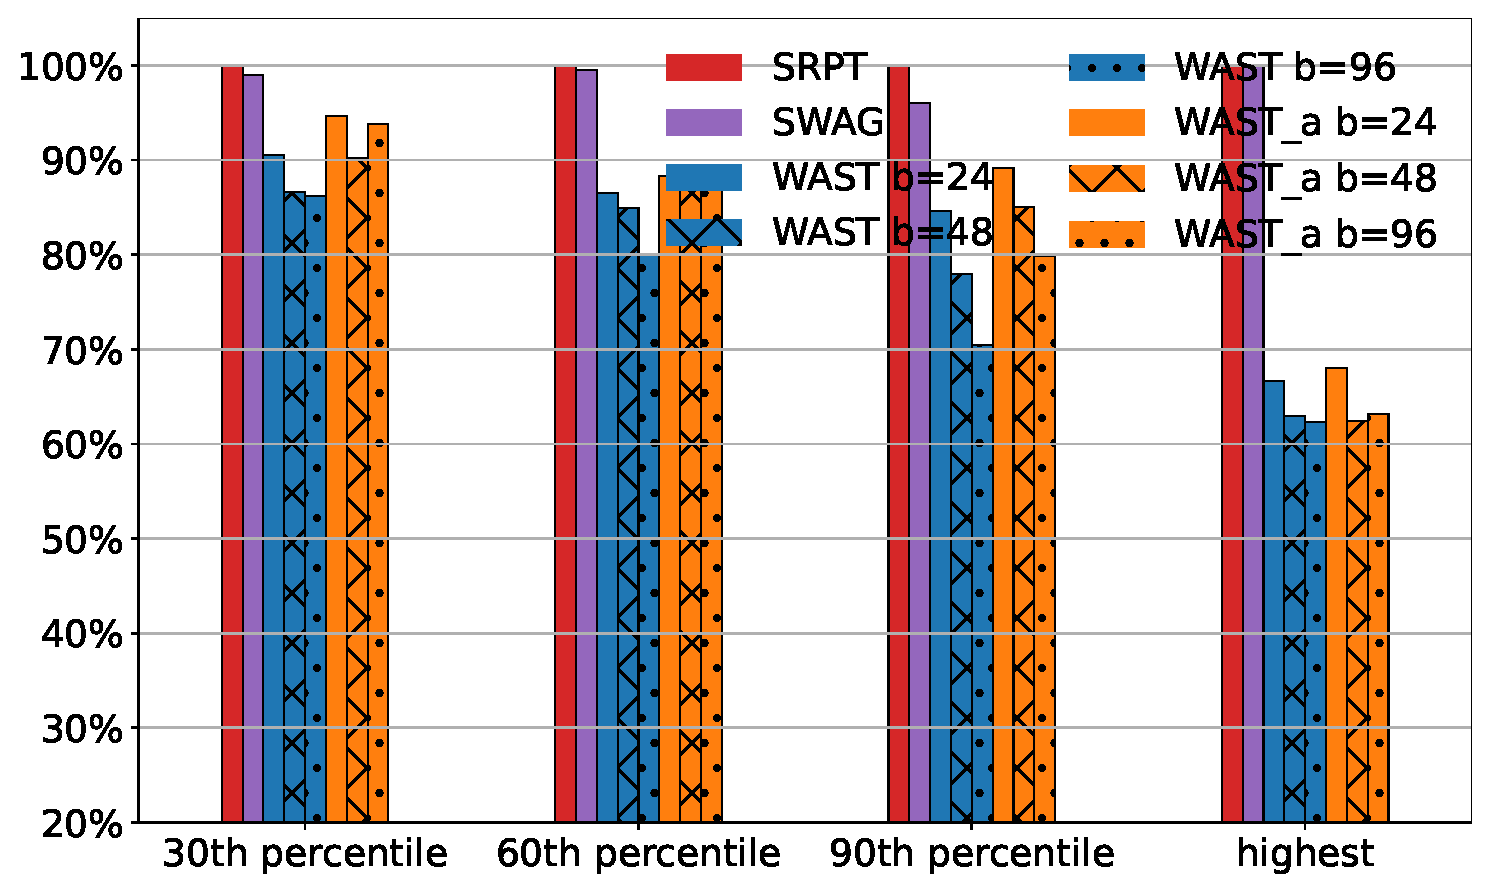
\includegraphics[width=0.24\textwidth]{Image2/CDFpercentile_Ali2018_4_70.eps}}%
\hfil
\subfloat[utilization = 80\%]
%
{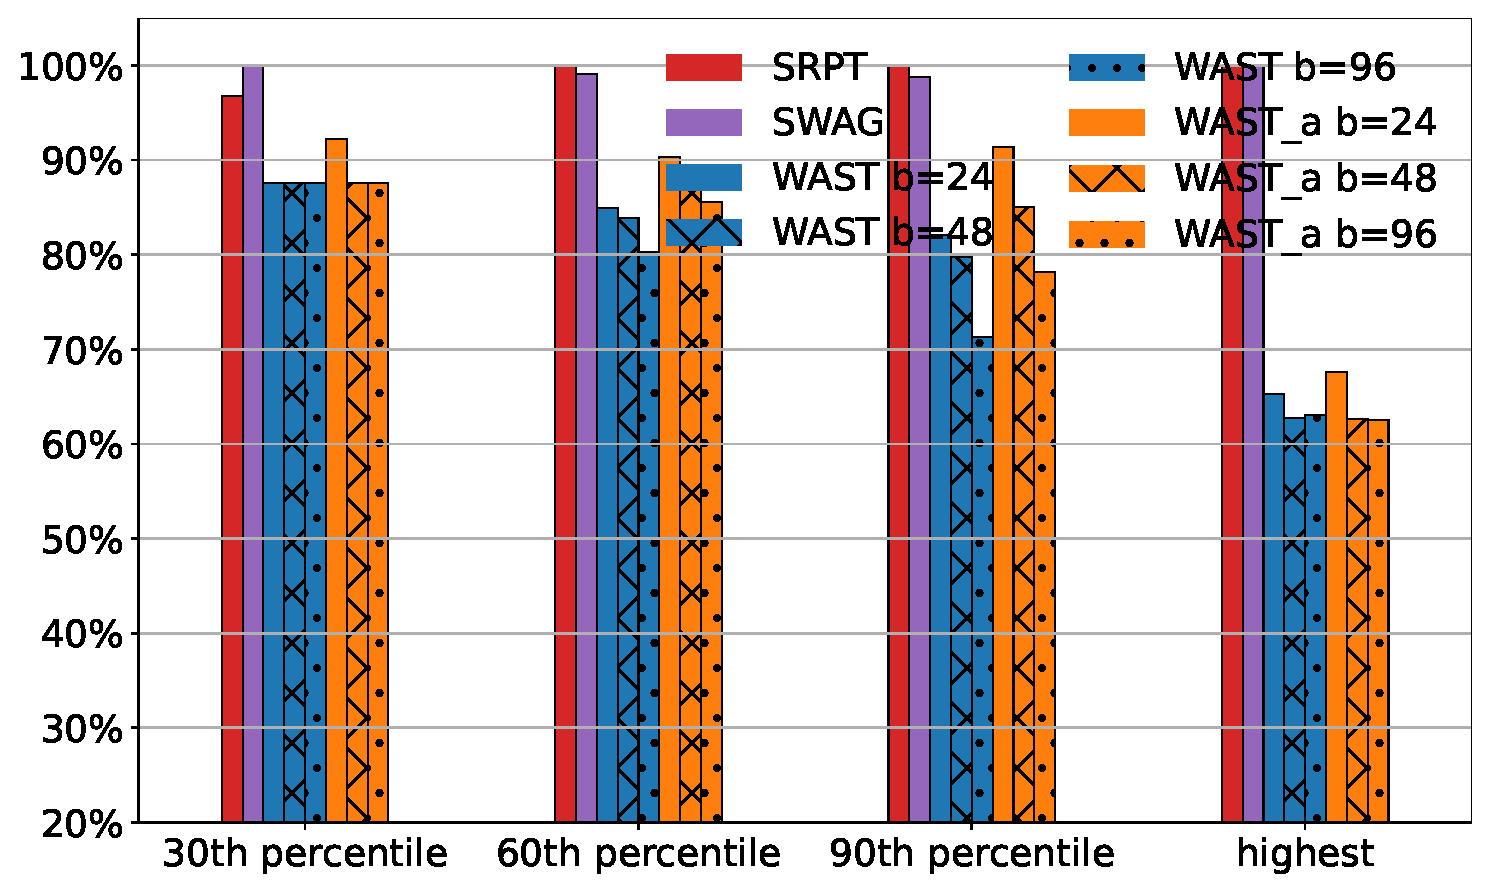
\includegraphics[width=0.24\textwidth]{Image2/CDFpercentile_Ali2018_4_80.eps}
%\label{Fg:eg2}
}
\caption{Job Response Time at Different Percentiles, Zipf Distribution $\alpha=1$, Alibaba 2018}
\label{fig:JRT_CDF2}
\end{figure*}

Tables \ref{tab:computation_time1} and \ref{tab:computation_time2} show the average computation time per recomputation of the SWAG, WAST and WAST\_a algorithms under various bandwidth settings, slot numbers per site, Zipf parameters $\alpha$ and system utilization. Due to space limitations, we present the results for the Alibaba 2018 trace under $60\%$ and $80\%$ utilization only. Both tables demonstrate that WAST\_a effectively reduces the computation time compared with WAST, which can be up to $87.3\%$. Furthermore, it can be seen that the average computation time of WAST is about an order of magnitude higher than that of SWAG, while the average computation time of WAST\_a is of the same order of magnitude as SWAG, demonstrating the effectiveness of WAST\_a in practice. %\textcolor{red}{We evaluated the computation time of both algorithms under different numbers of computing slots per server. The outcome shows that }% Under the $80\%$ utilization, the simulated duration from the first job's arrival to the last job's completion amounts to around 1.34 million seconds for the Alibaba 2017 trace and 0.4 million seconds for the Alibaba 2018 trace. In addition, the ratio of the average computation time to the average task duration is $1.1\%/0.4\%$ for two datasets in $80\%$ utilization and $0.4\%/0.2\%$ in $60\%$. This implies that during a single computation of WAST, the probability that a task execution finishes is very low. Taking the above factors together with the observation that the arrival of a new job generally has a trivial impact on the scheduling and transmission decision, we contend that the computational overhead of the WAST remains within an acceptable range, and preserving the existing job execution order and task transmission during the recomputation is a viable approach to mitigate the impact of this time cost.
%Therefore, we argue that the computation time of the algorithm has a negligible impact on the overall execution of the distributed system.

%The improvement becomes more pronounced when the workload distribution of jobs across sites is more skewed and when higher bandwidth is available, as the network resource can be more effectively utilized to mitigate job workload imbalances under these conditions. Moreover, the algorithm exhibits better performance on the Alibaba 2017 trace. This is attributable to the higher ratio of average task duration to average data partition size in 2017, which allows a greater number of tasks to be transmitted within the average task processing time, thereby providing additional opportunities to reduce job response time through task migration. Furthermore, the higher average task count per job in 2017 implies that, under highly uneven task distributions, more workload accumulates at individual sites, leading to increased response times if task migration is not applied. This, in turn, allows the algorithm to offload more tasks from peak-load sites, further enhancing response-time performance.

\begin{table}[t]
  \caption{Average computation time (second), Alibaba 2018 trace, 60\% utilization}
  \label{tab:computation_time1}
  \centering
  \scalebox{0.8}{%
    \begin{tabular}{ccccccccc}
      \toprule
      \multicolumn{3}{c}{} & \multicolumn{2}{c}{b = 24Mbps} & \multicolumn{2}{c}{b = 48Mbps} & \multicolumn{2}{c}{b = 96Mbps}\\ 
      slot & $\alpha$ & SWAG & WAST & WAST\_a  & WAST & WAST\_a & WAST & WAST\_a\\
      \midrule
      \multirow{4}{*}{32} 
      & 0.0 &  $0.0157$ & $0.1209$ & $0.0201$ & $0.1127$ &  $0.0199$ & $0.1005$& $0.0198$ \\
      & 0.5 &  $0.0184$ & $0.1323$ & $0.0323$ & $0.1167$ &  $0.0297$ & $0.1023$& $0.0274$\\
      & 1.0 &  $0.0253$ & $0.1805$ & $0.0453$ & $0.1327$ &  $0.0468$ & $0.1301$& $0.0424$ \\
      & 2.0 &  $0.0475$ & $0.3014$& $0.0756$ & $0.2283$ &  $0.0872$ & $0.1936$& $0.0877$\\
      \midrule
      \multirow{4}{*}{64} 
      & 0.0 &  $0.0306$ & $0.2293$& $0.0378$ & $0.2310$ &  $0.0399$ & $0.2283$ & $0.0376$\\
      & 0.5 & $0.0365$ & $0.2797$& $0.0585$ & $0.2467$ & $0.0653$ & $0.2330$& $0.0563$\\
      & 1.0 & $0.0502$ & $0.3646$ & $0.0883$ & $0.3281$ & $0.0781$ & $0.2867$& $0.0845$\\
      & 2.0 & $0.0885$ & $0.6217$& $0.1666$ & $0.5365$ & $0.1299$ & $0.4369$& $0.1482$\\
      \midrule
      \multirow{4}{*}{128} 
      & 0.0 &  $0.0772$ & $0.6290$& $0.0899$ & $0.6169$ &  $0.0928$ & $0.6057$& $0.0922$\\
      & 0.5 & $0.0876$ & $0.7265$& $0.1127$ & $0.7205$ & $0.1228$ & $0.6601$& $0.1341$\\
      & 1.0 & $0.1302$ & $0.9427$& $0.1459$ & $0.9012$ & $0.1565$ & $0.8432$& $0.1781$\\
      & 2.0 & $0.2068$ & $1.5751$& $0.2247$ & $1.4975$ & $0.2317$ & $1.3203$& $0.2493$\\
      \bottomrule
    \end{tabular}
    }
\end{table}

\begin{table}[t]
  \caption{Average computation time (second), Alibaba 2018 trace, 80\% utilization}
  \label{tab:computation_time2}
  \centering
  \scalebox{0.8}{%
    \begin{tabular}{ccccccccc}
      \toprule
      \multicolumn{3}{c}{} & \multicolumn{2}{c}{b = 24Mbps} & \multicolumn{2}{c}{b = 48Mbps} & \multicolumn{2}{c}{b = 96Mbps}\\ 
      slot & $\alpha$ & SWAG & WAST & WAST\_a  & WAST & WAST\_a & WAST & WAST\_a\\
      \midrule
      \multirow{4}{*}{32} 
      & 0.0 &  $0.0326$ & $0.2950$ & $0.0411$ & $0.2782$ &  $0.0398$ & $0.2543$ & $0.0393$\\
      & 0.5 &  $0.0402$ & $0.3212$ & $0.0785$ & $0.2879$ &  $0.0616$ & $0.2549$ & $0.0547$\\
      & 1.0 &  $0.0521$ & $0.4283$ & $0.1078$ & $0.3196$ &  $0.1100$ & $0.2513$ & $0.0905$\\
      & 2.0 &  $0.0964$ & $0.4826$& $0.1503$ & $0.5172$ &  $0.1785$ & $0.4501$ & $0.1746$\\
      \midrule
      \multirow{4}{*}{64} 
      & 0.0 &  $0.0667$ & $0.5337$& $0.0863$ & $0.5363$ &  $0.0891$ & $0.5340$ & $0.0818$\\
      & 0.5 & $0.0842$ & $0.6638$& $0.1378$ & $0.5871$ & $0.1483$ & $0.5706$ & $0.1266$\\
      & 1.0 & $0.1078$ & $0.8532$ & $0.2476$ & $0.7262$ & $0.1848$ & $0.6623$ & $0.2028$\\
      & 2.0 & $0.1816$ & $1.2361$& $0.3728$ & $1.1003$ & $0.2484$ & $0.9437$ & $0.2913$\\
      \midrule
      \multirow{4}{*}{128} 
      & 0.0 &  $0.1665$ & $1.3935$& $0.1963$ & $1.4098$ &  $0.2024$ & $1.4332$ & $0.2087$\\
      & 0.5 & $0.1947$ & $1.7591$& $0.2664$ & $1.6433$ & $0.2899$ & $1.6000$ & $0.3193$\\
      & 1.0 & $0.2715$ & $2.1885$& $0.3210$ & $2.0776$ & $0.3473$ & $1.8640$ & $0.3722$\\
      & 2.0 & $0.4260$ & $3.9332$& $0.4998$ & $3.6373$ & $0.5136$ & $3.0193$ & $0.5459$\\
      \bottomrule
    \end{tabular}
    }
\end{table}

\subsection{Evaluation on Robustness and Scalability}


\section{Discussion}
\textbf{Heterogeneous tasks.} In real-world workloads, a job may consist of tasks with heterogeneous processing times and data sizes. Our proposed model and algorithms are capable of handling heterogeneous tasks by replacing the parameters $l_k$ and $d_k$ with task-specific values. Although this complicates the modeling of computation and transmission process, it does not compromise the effectiveness of our proposed algorithms.

\textbf{Limited network resources.} Inter-datacenter bandwidth is often limited and costly compared to intra-datacenter links. Therefore, the scheduler must avoid excessive network resource consumption. We suggest that the algorithm should exclusively utilize the spare network bandwidth, which is identified based on current system conditions. The specific method for quantifying this spare bandwidth via network monitoring is beyond the scope of this paper.

\textbf{Replicated data inputs.} Cloud-based environments often replicate data chunks across multiple geo-distributed servers in order to reduce service response latency and data transfer overhead \cite{guan2022task, zhao2025data}. Our method can be integrated with algorithms that determine task assignments under replicated data inputs. Specifically, we first execute the task assignment algorithm to determine an initial execution site for each task, and then employ our proposed algorithm(s) to derive the job execution order and task transmissions. Notably, if a destination site is found to already host a replica of the required data partition, the corresponding transmission is not needed, and the task can be processed locally at the destination.

\section{Summary}
\label{sec:conclusion2}
In this chapter, we have proposed a WAST algorithm and a fast approximation to improve job scheduling efficiency in geo-distributed systems with the usage of network resources. WAST constructs a near-optimal job execution order with task transmissions progressively. In each round, WAST searches for the job with the minimum completion time among all unsettled jobs given the scheduled workloads and task transmissions of previous rounds. The sub-problem of minimizing a single job's completion time is converted into solving multiple minimum-cost flow problems, which can be computed efficiently. 
%Once the job is found, its computation load and transmissions are updated to the system, and the next round starts with the updated system computing and network resource usage conditions. The process repeats until all jobs are scheduled. 
We also present a fast approximation to WAST, which optimizes each job's completion time by transferring its tasks of the latest completion time to other sites recursively. We have evaluated WAST and its approximation using real job traces from Alibaba. The experimental results show that WAST can effectively reduce the average job response time, especially when the task distributions of jobs are highly skewed.
\chapter{Protective Scheduling for distributed Job Execution}
\label{ch:PFSP}
% \lipsum[50]
In this chapter, we focus on developing scheduling policies that improve job processing efficiency in terms of average job response time, while guaranteeing a certain criterion of long-term fairness for online distributed job execution, where each job's workload is distributed across multiple sites. Inspired by the concept of protective scheduling in the single site system introduced by Friedman \textit{et al.} \cite{friedman2003fairness, friedman2003protective}, our long-term fairness criterion dictates that no job should complete later than it would under a distributed Processor Sharing (PS) protocol, which evenly shares the site capacity among all active jobs at each site. Building on this foundation, we aim to develop job scheduling algorithms that tackle the dual challenges of enhancing processing efficiency while strictly adhering to this fairness criterion.


\section{Preliminaries}
\label{sec:prelim}
\subsection{Slack System in Single-Site Case}
\label{sec:pre_slack}

We introduce a slack system that provides an intuitive protectiveness assessment of the current system state, identifying whether any jobs are projected to exceed their completion times under the Processor Sharing (PS) policy. It is defined as follows \cite{friedman2003protective}:

Consider a single-site system with compute resources, where the total resource capacity is assumed to be $1$ for simplicity. During execution, the system hypothetically runs a Processor Sharing (PS) policy to obtain each job's PS completion time, which serves as its deadline. Every job in the system has two types of job loads, namely the real load and the PS load, which represent the remaining load of a job in the current system and the hypothetical PS execution respectively. Initially, the real load and the PS load of a new job are both equal to its initial load upon its arrival. The PS load then continuously decreases according to a simulated execution of the PS policy, where processing capacity is evenly shared by all jobs with positive loads, while its real load remains unchanged or decreases according to the actual scheduling policy. Let the current real loads and PS loads for $n$ jobs in the system be $w_1, w_2, \dots, w_n$ and $v_1, v_2, \dots, v_n$, respectively. For simplicity, the job sequence is sorted in ascending order of their PS loads, i.e., $v_1 \le v_2 \le \dots \le v_n$ (note that the PS load order is identical to the PS completion time order of the jobs). The slack of a job $J_i$ is computed as follows:
\begin{equation}
    \label{eq:slack_single}
    s_i = \sum_{l=1}^{i} v_{l} + (n-i)v_i- \sum_{l=1}^i w_l.
\end{equation}
Specifically, the slack $s_i$ consists of two parts: (i) the PS completion time of $J_i$, given by $\sum_{l=1}^{i} v_{l} + (n-i)v_i$, and (ii) the time required to complete the real loads of the first $i$ jobs, given by $\sum_{l=1}^i w_l$. Consequently, $s_i$ quantifies the maximum permissible delay for $J_i$ and its preceding jobs to complete before violating the deadline set at $J_i$'s PS completion time.

\subsection{Two Types of Events in Slack System}
\label{sec:Pre_TwoEvents}
We now explain how the slack system will change under various events. Friedman \textit{et al.} \cite{friedman2003protective} discussed the changes of the slack system under two types of events. First, if the system serves some job $J_i$ for a duration of $\Delta t$, the slacks of jobs preceding $J_i$ in the PS load order will decrease by $\Delta t$:
\begin{equation}
    s_l = s_l -\Delta t,\quad \forall l \in \{1, \dots, i-1\}.
\end{equation}
Second, if a new job arrives in the system and joins in the job sequence at the $i$-th position based on its PS load (suppose its initial load is $x$), it will cause the slacks of jobs preceding it to increase by $x$:
\begin{equation}
    s_l = s_l + x,\quad \forall l \in \{1, \dots, i-1\}.
\end{equation}
For both events, the slacks of subsequent jobs $J_{i+1}, J_{i+2}, \dots, J_n$ remain unchanged. 

\subsection{Servable and Completable jobs}
Friedman \textit{et al.} \cite{friedman2003protective} proved that a scheduling policy is protective if and only if the slack of each job remains non-negative at all times. In other words, once the slack of any job becomes negative, then regardless of subsequent scheduling decisions (in the absence of new job arrivals), at least one job will inevitably complete later than its completion time under the PS policy. Therefore, the analysis of the first type of event above (serving jobs) indicates that it may not be true that all jobs can be prioritized for processing immediately if the system aims to maintain protectiveness. This fundamental restriction introduces the concept of servability and completability. %Without loss of generality, we assume that the job sequence is sorted in ascending order of their PS loads: %For simplicity, in the following definition we assume that the job sequence is already sorted based on their PS loads.

%Consequently, avoiding negative slack implies that not all jobs can be prioritized for execution if the system aims to maintain protectiveness. This restriction naturally motivates the concepts of servability and completability. Without loss of generality, we assume that the job sequence is indexed in ascending order of their PS loads.

\begin{definition}
    A job $J_i$ is \textbf{servable} if and only if $s_{l} > 0$ for all $l \in \{1, \dots, i-1\}$.
\end{definition}

\begin{definition}
    A job $J_i$ is \textbf{completable} if and only if $s_{l} \ge w_{i}$ for all $l \in \{1, \dots, i-1\}$.
\end{definition}

%Note that the first job in the PS order ($i = 1$) is inherently servable and completable because the index set $\{1, \dots, i-1\} = \emptyset$, making the conditions vacuously true. Furthermore, if a job's real workload is completed but it remains in the system (i.e., its PS load is not yet cleared), its slack is set to infinity. This convention guarantees the computational integrity of servable and completable job states within the system.

%Friedman \textit{et al.} \cite{friedman2003protective} proved that a scheduling policy is protective if and only if the slack of each job remains non-negative throughout the time span. In other words, once the slack of any job becomes negative, then regardless of how jobs are subsequently scheduled (assuming no new job arrivals), at least one job will inevitably complete later than its completion time under the PS policy. Therefore, the analysis of the first type of event indicates that not all jobs can be processed first if the system goal includes keeping protectiveness. This introduces the concept of servability and completability. Assume the job sequence is sorted in ascending order of their PS loads already: %For simplicity, in the following definition we assume that the job sequence is already sorted based on their PS loads.

% \begin{definition}
%     A job $J_i$ is \textbf{servable}, if and only if $\forall l \in \{1, \dots, i-1\}, s_{l} > 0$.
% \end{definition}

% \begin{definition}
%     A job $J_i$ is \textbf{completable}, if and only if $\forall l \in \{1, \dots, i-1\}, s_{l} \ge w_{i}$.
% \end{definition}
Note that the first job in the PS load order is always servable and completable because the index set $\{1, \dots, i-1\}$ is empty for $i = 1$. Furthermore, a job that has actually completed its actual workload (its real load drops to $0$) but remains in the system—owing to an uncleared Processor Sharing (PS) load—is defined as both servable and completable, with its slack set to infinity. This convention ensures the correctness of the system's calculations regarding servable and completable jobs. 

\subsection{Fair Sojourn Protocol (FSP) and Its Variants}
Friedman \textit{et al.} \cite{friedman2003protective} proposed three protective scheduling policies in the single-site case, namely Fair Sojourn Protocol (FSP), Optimistic FSP (OFSP) and Pessimistic FSP (PFSP). FSP schedules jobs based on the PS load order (PS completion time order). OFSP and PFSP prioritize the servable job and the completable job with the least positive real load, respectively. Specifically, OFSP serves the servable job of the least real load until it completes or becomes not servable, and then repeats the computation of servable jobs to identify the next job to serve. Recall from Section 5.1.2 that when a new job arrives, the slacks of existing jobs either increase or remain unchanged. The term ``optimistic'' implies that although the job chosen by OFSP may not be able to serve to completion, the policy expects that there will be new job arrivals during its processing to further extend the PS completion time (and hence the slack) of the job, thus making it completable. On the contrary, the term ``pessimistic'' indicates that PFSP serves the job that is already completable (it stays completable if any new job arrives), which is more conservative and stable than OFSP.

%Note that the first job in the PS order is always servable and completable because the set $\{1, \dots, i-1\} = \emptyset$ for $i = 1$. In addition, a job with its real load completed while not removed from the system (i.e., its PS load is not completed yet) will have its slack set to infinity. This convention ensures the correctness of the system's computations regarding servable and completable jobs. In addition, the paper \cite{friedman2003protective} proved that a scheduling policy is protective if and only if the slack of each job is kept non-negative throughout the time span. In other words, once the slack of any job becomes negative, then no matter how the jobs are scheduled in the sequel (suppose no new job arrives), there must be at least one job who will finish later than its finish time under PS policy.

The following example illustrates how protective scheduling policies like FSP maintain long-term fairness and prevent job starvation compared to efficiency-targeted policies. Consider two jobs, $J_x$ and $J_1$, arriving simultaneously at $t=0$ with initial loads $w_x=2$ and $w_1=1$, respectively. Thereafter, a new job $J_{a+1}$ with an initial load of $1$ arrives at each subsequent time $t=a$ for $a = 1, 2, \dots, 100$.

If the system adopts an efficiency-targeted scheduling policy like Shortest Remaining Processing Time (SRPT), it will serve the jobs in the order of $J_1, \allowbreak J_2, \allowbreak \dots, \allowbreak J_{101}$, and finally $J_x$. This is because each job $J_a$ has a smaller load than $J_x$ and arrives exactly when the previous job $J_{a-1}$ completes. Consequently, $J_x$ will complete at $t=103$, suffering from severe starvation. 

Adopting FSP, the system execution will proceed as follows:

\begin{itemize}
    \item \textbf{$t=0$:} The system has $J_x$ and $J_1$ with initial loads of $2$ and $1$, respectively. The system prioritizes $J_1$ for processing.
    
    \item \textbf{$t=1$:} $J_1$ finishes its real execution, and $J_2$ arrives. In the hypothetical PS execution, the PS loads are $v_x=1.5$, $v_1=0.5$, and $v_2=1$. Since $J_1$ completes and $J_2$ has smaller PS load than $J_x$, the system chooses to serve $J_2$.
    
    \item \textbf{$t=2$:} $J_2$ finishes its real execution, and $J_3$ arrives. In the hypothetical PS execution, the PS loads are updated as $v_x \approx 1.167$, $v_1 \approx 0.167$, $v_2 \approx 0.667$, and $v_3=1$. The system then chooses to serve $J_3$.
    
    \item \textbf{$t=3$:} $J_3$ finishes its real execution, and $J_4$ arrives. Notably, during the interval $[2, 3]$, $J_1$'s PS load also drops to $0$ and is hence removed from the system. Therefore, the remaining PS loads become $v_x \approx 0.889$, $v_2 \approx 0.389$, $v_3 \approx 0.722$, and $v_4=1$.
\end{itemize}

At time $t=3$, there are four jobs remaining in the system and two of them still have real loads ($J_x$ and $J_4$). The system calculates that $J_x$ has a lower PS load than $J_4$ ($0.889 < 1$), so FSP chooses to serve $J_x$, preventing it from indefinite starvation.

%Now suppose the system adopts FSP instead. At $t=0$, the system has two jobs $J_x, J_1$ with PS load and real load $2, 1$ and it schedules $J_1$ first. At $t=1$, $J_1$ completes in real load and $J_2$ arrives, where the PS load becomes $v_x=1.5, v_1=0.5, v_2=1$, so the system chooses to serve $J_2$ first. Next, at $t=2$, $J_2$ completes in real load and $J_3$ arrives, where the PS load becomes $v_x=1.167, v_1=0.167, v_2=0.667, v_3=1$, and the system serves $J_3$. At $t=3$, $J_3$ completes in real load and $J_4$ arrives. Note that $J_1$ here also completes in PS load and is removed from the system. Therefore, the PS load becomes $v_x=0.889, v_2=0.389, v_3=0.722, v_4=1$, and the system chooses to serve $J_x$ now, which rescues it from starvation.

\section{System Model}
\label{sec:model}
Consider a distributed computing environment comprising $m$ distinct sites denoted by $\mathcal{S} = \{S_1, S_2, \dots, S_m\}$. Each site $S_j$ has compute resources with capacity $u_j$. A set of $n$ jobs $\mathcal{J} = \{J_1, J_2, ..., J_n\}$ are ready to run the system. Each job $J_i$ consists of workloads distributed across multiple sites that can be processed in parallel, and its overall completion time is determined by the workload that finishes last. %For simplicity, we use $[x]$ to represent the set $\{1, 2, \dots, x\}$ for a positive integer $x$. 
We describe the real load distribution of the jobs using a load matrix $W_{n\times m}$. Specifically, each element $w_{ij}$ represents the processing load of job $J_i$ at site $S_j$. For example, if $u_2=2$ and $w_{12}=4$, processing $J_1$'s load at $S_2$ will require $w_{12}/u_2=2$ time units to complete. Furthermore, the system simulates a Processor Sharing (PS) policy at each site to estimate both the site-specific and global PS completion times for every job. Under this simulated policy, each site equally shares its capacity among all jobs with positive loads on the site. To track this process, we introduce a virtual load matrix $V_{n\times m}$, where each element $v_{ij}$ denotes the virtual load of job $J_i$ at site $S_j$ under the PS policy, henceforth referred to as the PS load. The key notations used in this chapter are summarized in Table \ref{tab:Notation}. We aim to design scheduling policies that achieve the highest possible efficiency in terms of average job response time, while ensuring that every job can complete before its completion time under the PS policy. Note that although the model is formulated in a static setting, it can be extended to online scenarios by capturing snapshots of dynamic job load distributions. 

\begin{table}[tbp]
    \centering
    \caption{Notation Table}
    \label{tab:Notation}
    \begin{tabular}{cc}
        \toprule
        Notation & Definition \\
        \midrule
        $\mathcal M = \{S_1, S_2, \dots, S_m\}$ & Set of sites \\ 
        $\mathcal J = \{J_1, J_2, \dots, J_n\}$ & Set of jobs \\ 
        $u_1, u_2, \dots, u_m$                  & Each site's compute resource capacity \\
        $W_{n\times m}$                         & Real load matrix \\
        $V_{n\times m}$                         & PS load matrix \\
        \bottomrule
    \end{tabular}
\end{table}

\section{Distributed Slack System}
\label{sec:distributed_slack}
In this section, we discuss how to build a slack system in the distributed job execution case that assists us in the protectiveness assessment of the system and designing protective scheduling algorithms. There are two types of views in constructing the slack system: a global view and an independent view.

\subsection{Slack System in Distributed Job Execution Case: A Global View}
Since a job's global PS completion time is determined by the maximum of its site-specific PS completion times across all sites, an intuitive design of the slack system is to adopt each job's global PS completion time as the sorting criterion, which we refer to as the Global Slack ($GS$) scheme.

In the single-site case, computing the PS completion time requires jobs to be sorted in ascending order of their PS loads. However, in the distributed job execution case, the PS load distribution $V$ may give rise to different job sequences at different sites. For notational simplicity, let $P_j(i)$ denote the set of jobs that precede (and include) job $J_i$ when sorted in ascending order of their PS loads on site $S_j$:
\begin{equation}
    \label{eq:P_j(i)}
    P_j(i) = \bigl\{ J_k \in \mathcal{J} \;\big|\; (v_{kj}, k) \le (v_{ij}, i) \bigr\}
\end{equation}
where $\le$ denotes the standard lexicographical order on the tuples. In addition, different sites $S_j$'s in the system may have different resource capacities $u_j$'s. Thus, the site-specific PS completion time of a job $J_i$ at a site $S_j$ can be expressed as
\begin{equation}
    \frac{1}{u_j}\left(\sum_{J_l \in P_j(i)}v_{lj} + (n - |P_j(i)|)v_{ij} \right).
\end{equation}
The global PS completion time $PS_i$ of a job $J_i$ is the maximum site-specific PS completion time of $J_i$ across $m$ sites:
\begin{equation}
    PS_i = \max_{1\le j \le m} \frac{1}{u_j}\left(\sum_{J_l \in P_j(i)}v_{lj} + (n - |P_j(i)|)v_{ij}\right).
\end{equation}
Based on this, we can sort jobs in ascending order of their global PS completion times, i.e., $PS_1 \le PS_2 \le \dots \le PS_n$. After sorting, the slack of a job $J_i$ at site $S_j$ under the $GS$ scheme can be defined as:
\begin{equation}
    s_{ij} = PS_i - \frac{1}{u_j}\sum_{l=1}^i w_{lj},
\end{equation}
which is the difference between $J_i$'s global PS completion time and the time required to complete the real loads of the first $i$ jobs at site $S_j$. We refer to this slack as the $GS $slack. The $GS$ slack quantifies the maximum permissible delay for $J_i$ and its preceding jobs to complete before violating the deadline set at $J_i$'s global PS completion time. Under the $GS$ scheme, a scheduling policy is protective if and only if all $s_{ij}$'s are non-negative during the system execution. Similar to the single-site case (introduced in Section \ref{sec:Pre_TwoEvents}), serving job $J_i$ at site $S_j$ for a duration of $\Delta t$ reduces the $GS$ slacks of all preceding jobs ($P_j(i)\setminus J_i$) at $S_j$ by $\Delta t$, while a new job arrival will only increase the slacks of jobs in $P_j(i)\setminus J_i$ at $S_j$. The definitions of servable and completable jobs can also be applied to individual sites in the distributed job execution case. We define that a job is \textbf{servable} or \textbf{completable} globally if and only if it is servable or completable at all sites. Note that the completion of a job's real load at a particular site does not affect its global servability or completability. In addition, the first job in the global PS order is always servable and completable globally because the index set $\{1, \dots, i-1\}$ is empty for $i = 1$.

%Note that if a job has its real load completed at some site, this does not affect its global servability and completability. 
\subsection{Conflict of Global Order-based Scheduling to Protectiveness}
\label{sec:conflict}
An ideal job schedule naturally desires a global order that is consistent across all sites, which is intuitive, simple and guarantees efficiency (obviously policies that prioritize different jobs for processing at different sites will lead to worse job completion times). In protective scheduling, this necessitates an algorithm that generates a global job order in which every job is globally completable when scheduled for processing. However, we discover that under the $GS$ scheme, the protectiveness cannot be guaranteed if the system schedules jobs using a global job order. The primary reason is that during the execution, while the $GS$ scheme ensures that the deadline derived from the global PS completion time of each job can be satisfied, the site-specific PS completion time of some particular job $J_i$ at some particular site $S_j$ can be violated. Recall that the global PS completion time of a job is given by the maximum of its site-specific PS completion times across all sites. Since new jobs may arrive and new job arrivals can extend the site-specific PS completion times of jobs, it is possible that after some new jobs arrivals, this violated site $S_j$ decides the global PS completion time of job $J_i$, thereby making the slack $s_{ij}$ negative and violating protectiveness. We construct a concrete example below to illustrate the above.%The example below further illustrates this point. %the $IS$ scheme does not guarantee that such a globally completable job exists (so the system may not be able to find a valid schedule), and

Consider a distributed system of two sites, where the capacities of both sites are assumed to be $1$ for simplicity. Suppose two jobs $J_1$, $J_2$ are submitted to the system with initial load distribution:
\begin{equation}
    W = \begin{bmatrix} 2a & 2a+e \\ 2a+2e & 2a-e \end{bmatrix},
\end{equation}
where $a \gg e > 0$, $J_1$ has loads $2a$ and $2a+2e$ on sites $S_1$ and $S_2$ respectively, and $J_2$ has loads $2a+e$ and $2a-e$ on sites $S_1$ and $S_2$ respectively. The site-specific PS completion time can be computed as:
\begin{equation}
    \begin{bmatrix} 4a & 4a \\ 4a+2e& 4a-2e \end{bmatrix}.
\end{equation}
Therefore, the global PS completion time of the two jobs are $4a, 4a+2e$, respectively, which introduces the global PS order $J_1 \prec J_2$.

We compute the slack system based on the $GS$ scheme: $J_1$ is the first job in the global PS order, so its $GS$ slacks are $[4a - 2a=2a, 4a-(2a+e)=2a-e]$; $J_2$ is the second job in the global PS order, so its $GS$ slacks are $[4a+2e-2a - (2a+2e) =0, 4a+2e-(2a+e)-(2a-e)=2e]$. Therefore, the slack matrix is
\begin{equation}
    S = \begin{bmatrix} 2a & 2a-e \\ 0 & 2e \end{bmatrix}.
\end{equation}
In this case, the first job $J_1$ in the global PS order is globally servable and completable, while the second job $J_2$ is not completable because $s_{11} = 2a < w_{21} = 2a+2e$. Therefore, any scheduling policy that wants to derive a global job order while keeping the system protective will serve $J_1$ to completion first. Meanwhile, if we treat $S_2$ as an independent single site, another type of slacks can be calculated based on the discussion in Section \ref{sec:pre_slack} (we define it as "local slack" temporarily to differentiate it from the $GS$ slack): the site-specific PS completion times of $J_1$ and $J_2$ at $S_2$ are $4a$ and $4a-2e$, respectively. Thus, the local PS load order at $S_2$ is $J_2 \prec J_1$ and the local slacks of $J_1$ and $J_2$ at $S_2$ are $4a-(2a-e)-(2a+e)=0$, and $4a-2e-(2a-e)=2a-e$, respectively. This indicates that $J_2$ is locally completable at site $S_2$ while $J_1$ is not, and serving $J_1$ will make $J_2$'s local slack negative.

Suppose the system adopts the global PS order $J_1 \prec J_2$ to execute jobs. At time $t=2a$, the real load distribution and PS load distribution will be
\begin{equation}
    W = \begin{bmatrix} 0 & e \\ 2a+2e & 2a-e \end{bmatrix}, \quad V = \begin{bmatrix} a & a+e \\ a+2e & a-e \end{bmatrix},
\end{equation}
respectively. The $GS$ slacks of jobs do not change because the system serves the first job in the global PS order, and it is still protective. Meanwhile, serving $J_1$ continuously decreases the local slack of $J_2$ at $S_2$ and it becomes negative ($2a-e-2a=-e$) already.

Suppose at time $t=2a$, a new job $J_3$ arrives with initial loads $0$ and $a-2e$ on sites $S_1$ and $S_2$ respectively. Then, the real load distribution and PS load distribution become 
\begin{equation}
    W = \begin{bmatrix} 0 & e  \\ 2a+2e & 2a-e \\ 0 & a-2e \end{bmatrix}, \quad V = \begin{bmatrix} a & a+e \\ a+2e & a-e \\ 0 & a-2e \end{bmatrix},
\end{equation}
respectively. Therefore, the site-specific PS completion time is 
\begin{equation}
    \begin{bmatrix} 2a & 3a-2e \\ 2a+2e & 3a-4e \\ 0 & 3a-6e \end{bmatrix}. 
\end{equation}

Since $a \gg e$, the global PS completion times of all three jobs are decided by site $S_2$, and the global PS order becomes $J_3 \prec J_2 \prec J_1$, and the $GS$ slacks of jobs are 
\begin{equation}
    S = \begin{bmatrix} a-4e & 0 \\ a-6e & -e \\ 3a-6e & 2a-4e \end{bmatrix},
\end{equation}
where $s_{22}$ is negative. This implies that $J_2$ will never be able to complete its load at site $S_2$ before its global PS completion time. Therefore, the protectiveness is violated at the arrival of $J_3$. %Here $J_3$ and $J_2$ have the same global PS completion time, but exchanging them in the global PS order derives the same conclusion.

As demonstrated by the above example, global order-based scheduling policies fail to preserve the protectiveness in distributed environments under the $GS$ scheme. Furthermore, if the local slack of any job $J_i$ at a site $S_j$ becomes negative, one can systematically construct a worst-case scenario involving the simultaneous arrival of a job set $\{J_{(1)}, J_{(2)}, \dots, J_{(z)}\}$, each containing a load $x \le v_{ij}$ at $S_j$ ($v_{ij}$ is the PS load of $J_i$ at $S_j$) and zero load at all other sites. Under such conditions, the site-specific PS completion time of $J_i$ at $S_j$ can be arbitrarily delayed while its local slack keeps negative (i.e., the second type of events $2$ in Section \ref{sec:Pre_TwoEvents}). For a sufficiently large $z$, this prolonged site-specific PS completion time will become the global PS completion time of $J_i$, thereby rendering its $GS$ slack at $S_j$ negative. This fundamental limitation highlights strciter constraints on the slack system to maintain protectiveness, which we will introduce next.
%two prospective paradigms for the design of protective policies: (i) adopting order-independent strategies—such as proportional capacity allocation among a designated job subset or time-slicing execution—which inevitably introduces implementation overhead and may compromise aggregate processing efficiency; or (ii) formulating an alternative slack scheme that facilitates the robust design of protective scheduling mechanisms. %\textcolor{blue}{This fundamental limitation indicates a stronger constraint requirement on the slack system in order to preserve protectiveness, which we will introduce next.}

\subsection{Slack System in the Distributed Job Execution Case: An Independent View}
Another natural approach to extend the slack system to distributed environments is to compute the slack at each site independently, which we refer to as the Independent Slack ($IS$) scheme. Under the $IS$ scheme, we do not derive the global PS order, and each site performs slack calculations independently. Using the notation $P_j(i)$ defined in equation \ref{eq:P_j(i)} for the set of jobs preceding (and including) $J_i$ based on their PS loads at $S_j$, the slack of job $J_i$ at site $S_j$ under the $IS$ scheme is defined as:
\begin{equation}
    \label{eq:slack_IS}
    s_{ij} = \frac{1}{u_j}\left(\sum_{J_l \in P_j(i)}v_{lj} + (n - |P_j(i)|)v_{ij} - \sum_{J_l \in P_j(i)}w_{lj}\right).
\end{equation}
We refer to this slack as the $IS$ slack. Similar to the $GS$ scheme, a protective scheduling algorithm in the $IS$ scheme requires that every $s_{ij}$ to be non-negative during the system execution, i.e., the actual completion time of each job at every site does not exceed its site-specific PS completion time. Compared with the $GS$ scheme, the $IS$ scheme appears to be a stricter constraint since the completion deadline is set for each site rather than for the system as a whole. Consequently, the global completion time of each job is also bounded by its global PS completion time, and protectiveness is guaranteed. The potential drawback of the $IS$ scheme is that scheduling policies following it may prioritize different jobs for processing at different sites (i.e., a global order of job execution may not exist), leading to poor efficiency in terms of average job response time. 


\section{PFSP\_x: A Trade-off Algorithm Framework}
\label{sec:PFSP_x}
Through the above analysis, we have shown a dilemma in distributed protective scheduling: adopting the $GS$ scheme can achieve higher efficiency by deriving global job processing orders, but it may violate the protectiveness. On the other hand, using the $IS$ scheme can guarantee the protectiveness, but may lead to poor efficiency because it may prioritize different jobs for processing at different sites. The key to solving this dilemma is to use the $IS$ scheme and keep the $IS$ slack of each job at each site non-negative while adjusting the schedule to approximate the global job processing order that is optimized for efficiency.% Based on this insight, we propose a novel heuristic algorithm framework PFSP\_x which combines the independent slack system with any globally order-based scheduling policy to enhance efficiency while maintaining protectiveness.

\subsection{PFSP\_x}
We propose a novel heuristic algorithm framework PFSP\_x which combines the Independent Slack scheme with any global order-based scheduling policy to enhance efficiency while maintaining protectiveness. Specifically, PFSP\_x takes as input a global job processing order derived by any efficiency-targeted scheduling policy like SRPT or Workload-Aware Greedy Selection (SWAG) \cite{hung2015scheduling}, which is treated as the hint order for job processing and tries to approximate to it in the schedule. PFSP\_x computes the $IS$ slack of each job at each site $S_j$ independently, from which it calculates the set of locally completable jobs and schedules the job with the highest priority in the hint order for processing, updates the $IS$ slacks until all jobs at site $S_j$ are scheduled. Algorithm \ref{alg:PFSP_x} illustrates the details of the procedure at one site. The algorithm runs at each site based on the site-specific information, i.e., capacity, real loads and PS loads.


\begin{algorithm}[t]
  \caption{PFSP\_x Algorithm at Individual Sites}\label{alg:PFSP_x}
  
  \KwIn{A set of jobs $\mathcal{J} = \{J_1, J_2, \ldots, J_n\}$ with real loads $w_1, w_2, \dots, w_n$ and PS loads $v_1, v_2, \dots, v_n$, hint order $\mathbf{h}$.}
  \KwOut{Job execution order.}
  \BlankLine
  
  Let jobs be sorted in ascending order of PS load, i.e., $v_1 \le v_2 \le \dots \le v_n$\;
  $\sigma \leftarrow 0$\;
  \BlankLine
  
  \For{$i = 1$ \KwTo $n$}{
      $\sigma \leftarrow \sigma + v_i - w_i$\;
      $s_i \leftarrow \sigma + (n-i)v_i$\;
      $r_i \leftarrow \begin{cases} \infty, & \text{if } i = 1; \\ \min(r_{i-1}, s_{i-1}), & \text{otherwise}; \end{cases}$
  }
  \BlankLine

  \While{$\mathcal{J} \neq \emptyset$}{
      $\mathcal{C} \leftarrow \{J_i \in \mathcal{J} \mid r_i \ge w_{i} \}$\;
      $J_y \leftarrow \operatorname*{argmin}_{J_i \in \mathcal{C}} \text{pos}(J_i, \mathbf{h})$\;
      Append $J_y$ to the job execution order\;
      $\mathcal{J} \leftarrow \mathcal{J} \setminus \{J_y\}$\;
      \BlankLine

      \For{$i = 1$ \KwTo $y-1$}{
          $s_i \leftarrow s_i - w_{y}$\;
      }
      $s_{y} \leftarrow \infty$\;
      \BlankLine

      \For{$i = 1$ \KwTo $n$}{
          $r_i \leftarrow \min(r_{i-1}, s_{i-1})$\;
      }
  }
  \BlankLine
  \Return Job execution order\;
\end{algorithm}

At every single site, PFSP\_x sorts jobs in ascending order of their PS loads, computes each job's $IS$ slack $s_i$ and the minimum slack $r_i$ of jobs preceding each job (lines 3-6). Because computing the $IS$ slack requires the cumulative PS load and real load of preceding jobs, a running variable $\sigma$ is used to record the sum and optimize computing complexity. Note that a job $J_i$ is completable if and only if its real load $w_i$ is smaller or equal to the $IS$ slacks of all its preceding jobs, which is equivalent to $r_i \ge w_i$. Next, the algorithm calculates the set of completable jobs $\mathcal{C}$ (line 8) by judging whether $r_i \ge w_i$ for each unscheduled job $J_i$. Then, it schedules the job with the highest priority in the hint order (line 9). Here, we define $\text{pos}(J_i, \mathbf{h})$ as the position (index) of job $J_i$ within $\mathbf{h}$, where $\mathbf{h}$ is the hint order (permutation) of jobs given as input. A lower position index indicates a higher priority. Then, the algorithm appends the selected job $J_y$ to the job processing order of the local site (line 10) and removes $J_y$ from consideration (line 11). After scheduling $J_y$, the algorithm updates all $s_i$'s and $r_i$'s (lines 12-16). For each job before $J_y$ in the PS load order, its $IS$ slack decreases by $w_y$; the $IS$ slakc $s_y$ of job $J_y$ becomes infinity; for each job after $J_y$ in the PS load order, its slack remains unchanged. After updating all the $IS$ slacks, the algorithm updates $r_i$'s. The scheduling repeats iteratively until all jobs are scheduled. Finally, the algorithm returns the job execution order of the local site. In this way, PFSP\_x achieves both the protectiveness guarantee by following the $IS$ scheme and the efficiency improvement by approximating the hint order derived from any efficiency-targeted scheduling policy.

%, where each row $X_{j,*}$ represents the job scheduling order of site $S_j$, and each element $x_{ji}$ denotes the  job index of the $i$-th job in the schedule of $S_j$
% Note that based on the definition of slack in the single site case, we have $s_i - s_{i-1} = \sum_{l=1}^{i} v_{l} + (n-i)v_i- \sum_{l=1}^i w_l - (\sum_{l=1}^{i-1} v_{l} + (n-i+1)v_{i-1}- \sum_{l=1}^{i-1} w_l) = (v_i-v_{i-1})(n-i+1) - w_i$. Therefore, $s_i = s_{i-1} + (v_i-v_{i-1})(n-i+1) - w_i$. In addition, a job is completable if its real load is smaller or equal to slacks of its preceding jobs in the PS load order, so it should also be smaller or equal to the minimum $r_i$ among these slacks. 
%Note that PFSP\_x serves the globally completable job with the highest priority in the target job order at each site, which is expected to achieve better efficiency than PFSP\_i while keeping protective, although it does not guarantee to achieve better efficiency than PFSP\_g.
%, which reduces the computation on the slack of a job to $O(1)$

\subsection{Complexity Analysis}
In Algorithm \ref{alg:PFSP_x}, sorting $n$ jobs in ascending order of their PS loads takes $O(n\log n)$ time. To efficiently compute the slack of each job, we maintain and reuse a running cumulative sum $\sigma$, which aggregates the differences between the PS loads and real loads of jobs iteratively. Consequently, evaluating all slacks $s_i$ and the minimum preceding slacks $r_i$ can be achieved in $O(n)$ time. Thus, the total time complexity for the initial slack calculation of all $n$ jobs is $O(n \log n)$. Next, the algorithm iterates $n$ times, in which it computes the set of completable jobs $\mathcal{C}$ and searches for the completable job with the highest priority in the hint order $\mathbf{h}$. The former operation requires checking whether $r_i \ge w_i$ for each unscheduled job $J_i$, which takes $O(n)$ time. Selecting the job with the highest priority in $\mathbf{h}$ also takes $O(n)$ time. After scheduling the selected job, updating the slack $s_i$'s and minimum preceding slack $r_i$'s of all jobs takes $O(n)$ time. Therefore, the overall time complexity of Algorithm \ref{alg:PFSP_x} is $O((n \log n + n^2)) = O(n^2)$. The algorithm runs at each site. Since the runs at different sites are entirely independent, they can be parallelized in real-world deployments.%, effectively reducing the wall-clock computational complexity back to $O(n^2)$.
%Furthermore, since the computation at each site can be executed fully in parallel, the local time complexity at each individual site is reduced to $O(n^2)$.
%The former operation involves checking each job against its predecessors. \textcolor{blue}{By maintaining the minimum slack of preceding jobs, this takes $O(1)$ time for one job;} 

\subsection{Deployment}
\label{sec:deploy}
The PFSP\_x algorithm is highly amenable to deployment in real-world distributed computing environments, either via a centralized scheduler or through distributed execution. Initially, the system requires collecting the real load and PS load distributions of each job across sites, and running an efficiency-targeted scheduling policy to derive the hint job order $\mathbf{h}$. If the system deploys PFSP\_x at the central scheduler, the scheduler will compute the job processing orders of all sites by running Algorithm \ref{alg:PFSP_x} for each site separately and then propagate the job processing orders to respective sites .Alternatively, in a distributed setup, the central scheduler only broadcasts the hint order $\mathbf{h}$ to all sites. Each site independently performs its local $IS$ slack calculations and the scheduling logic, reducing network communication overhead and allowing for efficient scheduling in large distributed systems. Re-computation only needs to be triggered upon new job arrivals, while completed jobs are excluded from computation.


\section{Experiments}
\label{sec:experiment}

%Simulation experiments using read-world job traces are conducted to evaluate the performance of applying our scheduling algorithms to online scenarios as discussed in Section \ref{sec:deploy}.
This section evaluates the performance of our proposed protective scheduling algorithms in online scenarios through comprehensive simulations using real-world job traces, aligning with the deployment framework outlined in Section \ref{sec:deploy}.

\subsection{Datasets}
\begin{figure}[b]
\centering
\subfloat[Alibaba 2017]
{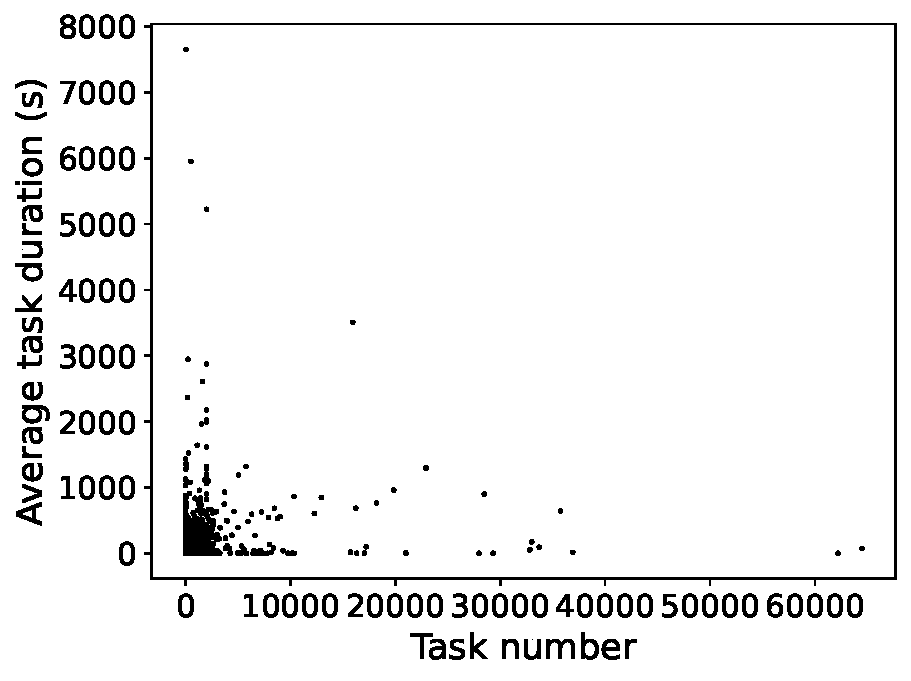
\includegraphics[width=0.47\linewidth]{Image3/JobDistribution_Ali2017_start=0_2D.pdf}%
%\label{fig_second_case}
%\label{Fg:eg1}
}
\hfil
\subfloat[Alibaba 2018]
%
{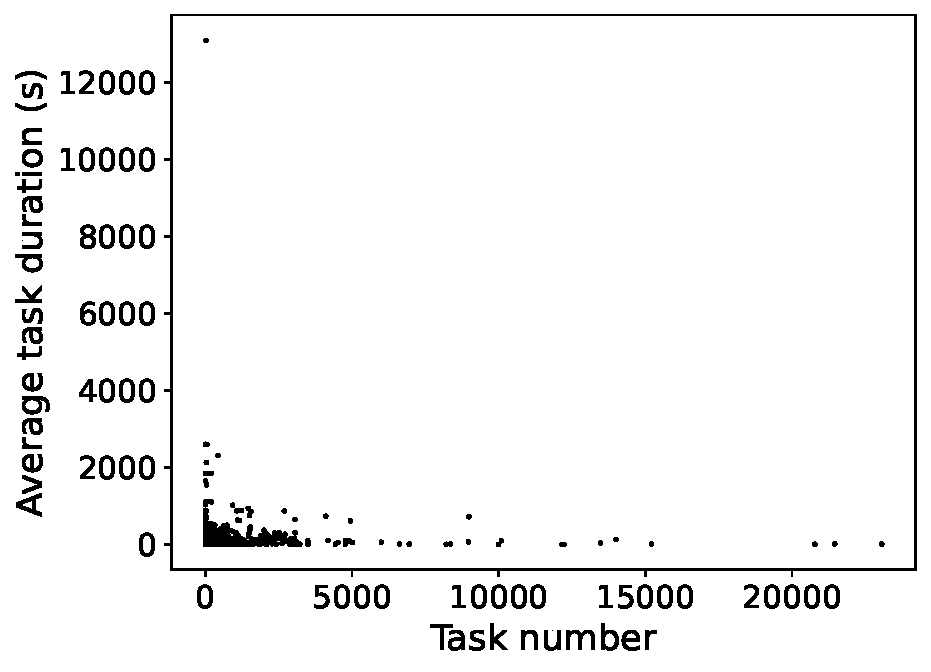
\includegraphics[width=0.48\linewidth]{Image3/JobDistribution_Ali2018_4_start=15000_2D.pdf}%
%\label{Fg:eg2}
}
\caption{Job characteristic distributions of segments sampled from two datasets}
\label{fig:distribution}
\end{figure}
To validate our approach under realistic production conditions, we utilize industrial cluster data from the Alibaba Cluster Trace Program \cite{Ali2017}. We extract essential scheduling telemetry from the raw log files of the 2017 and 2018 releases, capturing the arrival timestamp, task count, and processing duration of each job. From these pre-processed traces, a contiguous segment of 10,000 jobs is randomly sampled from each year to serve as the benchmark driving our simulations. As visualized in Fig. \ref{fig:distribution}, both segments sampled feature a heavy-tailed profile, where a tiny fraction of jobs dominates the vast majority of the total computational demand. Finally, the macro-level characteristics of the segments sampled for experimentation—including mean task counts and average task processing times—are summarized in Table \ref{tab:average_characteristic}.

\begin{table}[t]
    \centering
    \caption{Job characteristics of segments sampled from two datasets}
    \label{tab:average_characteristic}
    \begin{tabular}{ccc}
        \toprule
        Characteristics & Alibaba 2017 & Alibaba 2018 \\
        \midrule
        Average task number per job & $260.11$ & $94.70$ \\
        \midrule
        Average task processing time (s) & $209.18$ & $82.41$ \\
        \bottomrule
    \end{tabular}
\end{table}


\subsection{System Configuration}
We model a distributed environment comprising $m$ identical sites, where each site is provisioned with an equal capacity. To evaluate our algorithms under varying degrees of skewness in workload distribution, we initialize the initial load distribution of each job by deploying its tasks among the sites based on the Zipf distribution and summing up their task processing times at each site. Specifically, the task allocation across sites follows the proportional weights $1, 2^{-\alpha}, 3^{-\alpha}, \dots, m^{-\alpha}$, where the skewness parameter $\alpha$ controls the load imbalance. A higher $\alpha$ value implies that tasks are more heavily concentrated on a small subset of sites, while $\alpha = 0$ indicates a uniform distribution. We evaluate four distinct load distributions by varying $\alpha \in \{0.0, 0.5, 1.0, 2.0\}$. To prevent global load hotspots, we shuffle the order of the sites when deploying each job's task distribution. Additionally, the job arrival times from the trace are linearly scaled to emulate different system utilizations. While we examined various combinations of site numbers, site capacities, and load levels—all yielding consistent performance trends-we focus on presenting the results for a representative setup of $m = 10$ sites, capacity $u=32$ for each site, and $50\%$, $60\%$, $70\%$, and $80\%$ system utilizations.
%We simulate a distributed system of $m$ sites, each with the same number of $32$ computing slots. Each task is assumed to take up one computing slot to run and release it after completion. Due to the switching overhead consideration, we assume that the system does not allow preemption during task execution. For each job, the initial load distribution is generated by randomly deploying its tasks among the sites based on the Zipf distribution and summing up their task processing times: the numbers of tasks placed at the $m$ sites are proportional to $1, \frac{1}{2^\alpha}, \frac{1}{3^\alpha}, ..., \frac{1}{m^\alpha}$, where $\alpha$ is a Zipf parameter. A higher $\alpha$ implies a more skewed distribution (a higher proportion of tasks are concentrated at fewer sites), whereas $\alpha$ = $0$ indicates a uniform distribution. In the experiments, we test four Zipf distributions with $\alpha$ set to $0$, $0.5$, $1$ and $2$ to simulate different task distributions of jobs. After the load distribution is generated, we shuffle the order of the sites when deploying each job's load distribution, so that the total workload at each site will be roughly balanced. We scale the arrival times of the jobs in the datasets to simulate different levels of overall system utilization. We experiment with different numbers of sites, different numbers of computing slots per site, and different levels of system utilization, and the results show similar performance trends. Due to space limitations, we focus on presenting the results for $m=10$ sites, 32 computing slots per site, and system utilization = $50\%$, $60\%$, $70\%$ and $80\%$.


\subsection{Baseline Policies}
We implemented the following baseline policies in the experiments for comparison. The first two baselines are efficiency-targeted policies, namely Shortest Remaining Processing Time (SRPT) and Workload-Aware Greedy Scheduling (SWAG) \cite{hung2015scheduling}. SRPT executes jobs based on their estimated completion time in the case that each job runs alone in the system. In our distributed environment, the estimated completion time of a job $J_i$ is computed as $\max_{j \in[m]} w_{ij}/u_j$ where $w_{ij}$ is the remaining real load of $J_i$ at site $S_j$ and $u_j$ is the capacity of $S_j$. SRPT derives the job execution order by sorting these estimated completion times from low to high. SWAG schedules jobs in a greedy and iterative manner by estimating their completion times based on scheduled workloads in the system. After a job is scheduled, SWAG updates the scheduled workloads at all sites, and estimates the completion times of unscheduled jobs based on the updated workloads. We evaluate PFSP\_SWAG which uses the job execution order derived by SWAG as the hint order $\mathbf{h}$.

In addition, we extend the protective scheduling algorithms in the single-site case (FSP, PFSP and OFSP) to the distributed job execution case based on both of the slack schemes. Under the $IS$ scheme, we have FSP\_i, OFSP\_i and PFSP\_i, which runs FSP, OFSP and PFSP independently at each site. Similarly, under the $GS$ scheme, FSP\_g derives the global job execution order based on the global PS completion times, while OFSP\_g and PFSP\_g prioritize the globally servable or completable job that finishes the fastest if served first, respectively. Since the first job in the global PS order is always servable and completable, OFSP\_g and PFSP\_g are feasible. However, they cannot perfectly guarantee protectiveness, as in the counterexample of Section \ref{sec:conflict}. %For all the policies mentioned, the average time of computing the solution during the simulation is around $10^{-5}$ seconds.

The following example further illustrates how FSP\_g, OFSP\_g and PFSP\_g work in the distributed job execution case. Consider a distributed system of two sites $S_1$ and $S_2$, both with capacity $1$. Suppose at the beginning $t=0$, two jobs $J_1$ and $J_2$ are submitted to the system, with the initial load distribution 
\begin{equation}
    W = \begin{bmatrix} 8 & 9 \\ 10 & 7 \end{bmatrix},
\end{equation}
where $J_1$ has loads $8$ and $9$ on $S_1$ and $S_2$, respectively, and $J_2$ has loads $9$ and $7$ on sites $S_1$ and $S_2$ respectively. The site-specfic PS completion times of the jobs are
\begin{equation}
    \begin{bmatrix} 16 & 16 \\ 18 & 14 \end{bmatrix}.
\end{equation}
Thus, the global PS completion times of $J_1$ and $J_2$ are $16$ and $18$, respectively, and the global PS order is $J_1 \prec J_2$. Therefore, FSP\_g will serve $J_1$ first then $J_2$ at all sites, and the average job response time is $(9+18)/2=13.5$.

We compute the slack system based on the $GS$ scheme: $J_1$ is the first job in the global PS order, so its $GS$ slacks are $[16 - 8=8, 16-9=7]$; $J_2$ is the second job and its $GS$ slacks are $[18 - 10 - 8=0, 18-7-9=2]$, resulting in 
\begin{equation}
    S = \begin{bmatrix} 8 & 7 \\ 0 & 2 \end{bmatrix}
\end{equation}
 In this case, $J_1$ is globally servable and completable, while $J_2$ is not completable because $s_{11} = 8 < w_{21} = 10$. Therefore, PFSP\_g will behave the same as FSP\_g, i.e. serve $J_1$ to completion, and then $J_2$. Meanwhile, $J_2$ is servable since its preceding job $J_1$ has positive slacks $s_{11}=8>0, s_{12}=7>0$ at all sites. $J_2$ will finish at time $t=10$ if it is served first, while $J_1$ will finish at time $t=9$ if it is served first. Therefore, although both jobs are servable, OFSP\_g will also first serve $J_1$ to completion since it finishes earlier than $J_2$, and the average job response time is also $13.5$. 
%In this case, OFSP\_g can serve either of them. Note that if OFSP\_g chooses to serve $J_2$, it can only be served for $7$ seconds because $J_1$'s slack at site $S_2$ decreases to $0$ at $t=7$; After that, OFSP\_g turns to serve $J_1$ instead since $J_1$ becomes the only servable job in the system. When $J_1$ finishes, OFSP\_g turns back to $J_2$ and serve it until $J_2$ finishes. This will result in the average job response time of $(16+17)/2=16.5$.

\subsection{Experimental Results}

\begin{figure*}[t]
    \centering
    \begin{subfigure}[b]{0.4\textwidth}
        \centering
        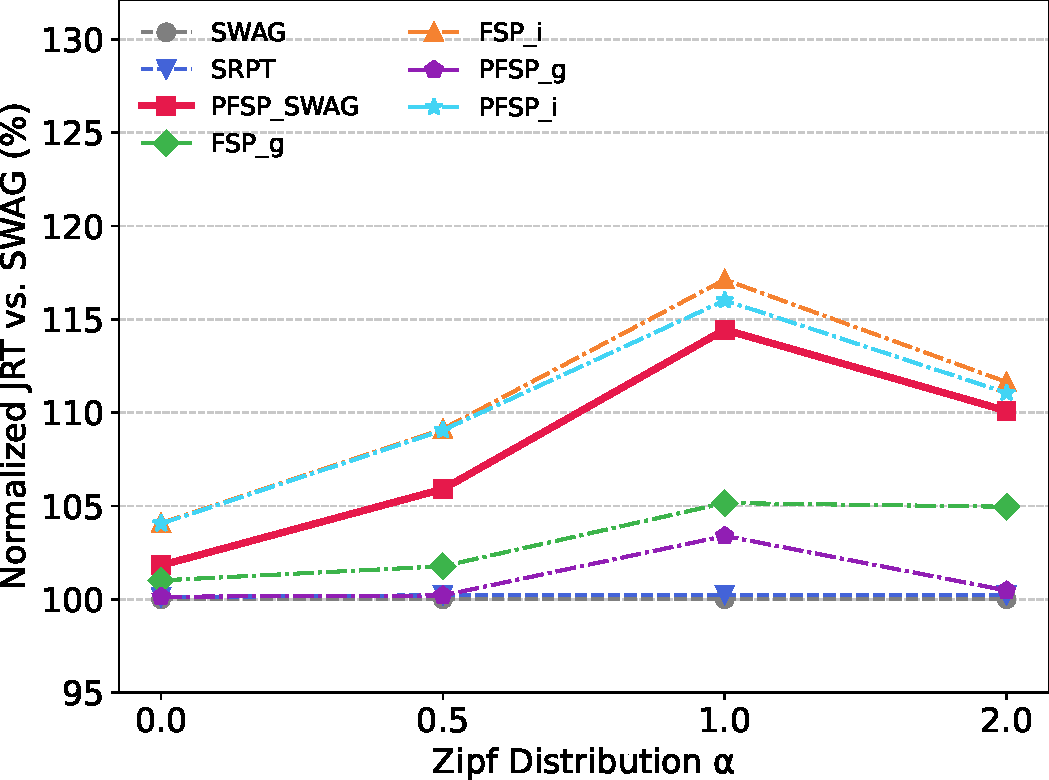
\includegraphics[width=\textwidth]{Image3/Workload_Ali2017_50_Dev=0.0.pdf}
        \caption{Utilization = 50\%}
    \end{subfigure}
    \hfill
    \begin{subfigure}[b]{0.4\textwidth}
        \centering
        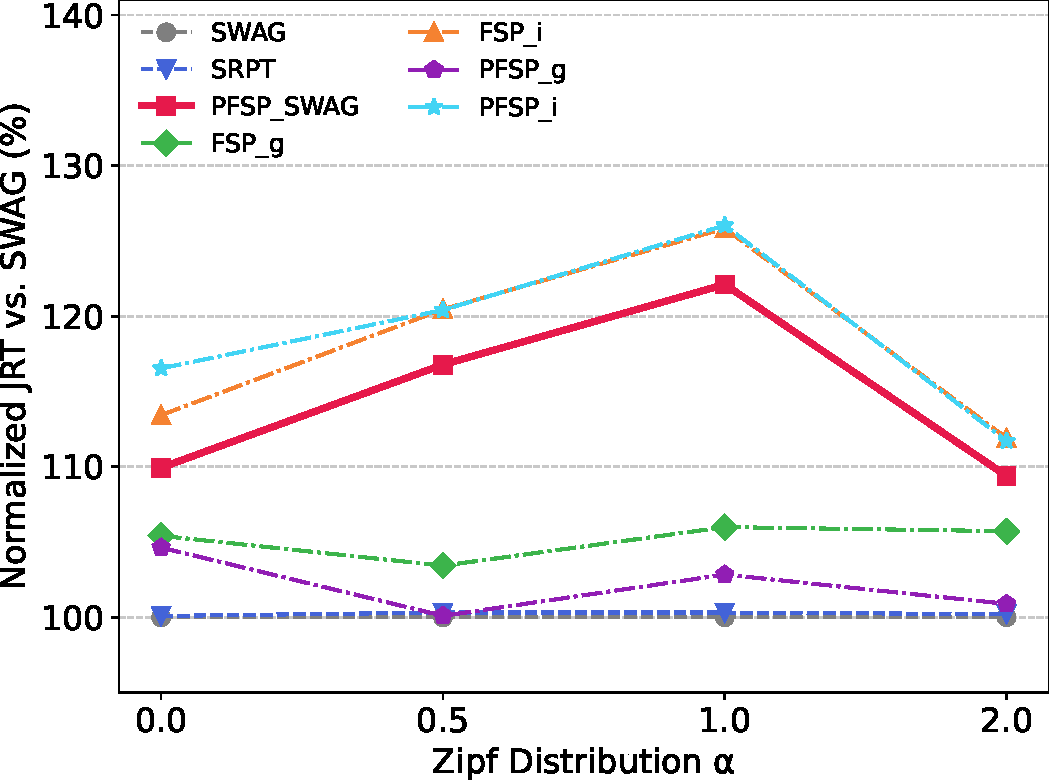
\includegraphics[width=\textwidth]{Image3/Workload_Ali2017_60_Dev=0.0.pdf}
        \caption{Utilization = 60\%}
    \end{subfigure}
    \vspace{0.8em}
    \begin{subfigure}[b]{0.4\textwidth}
        \centering
        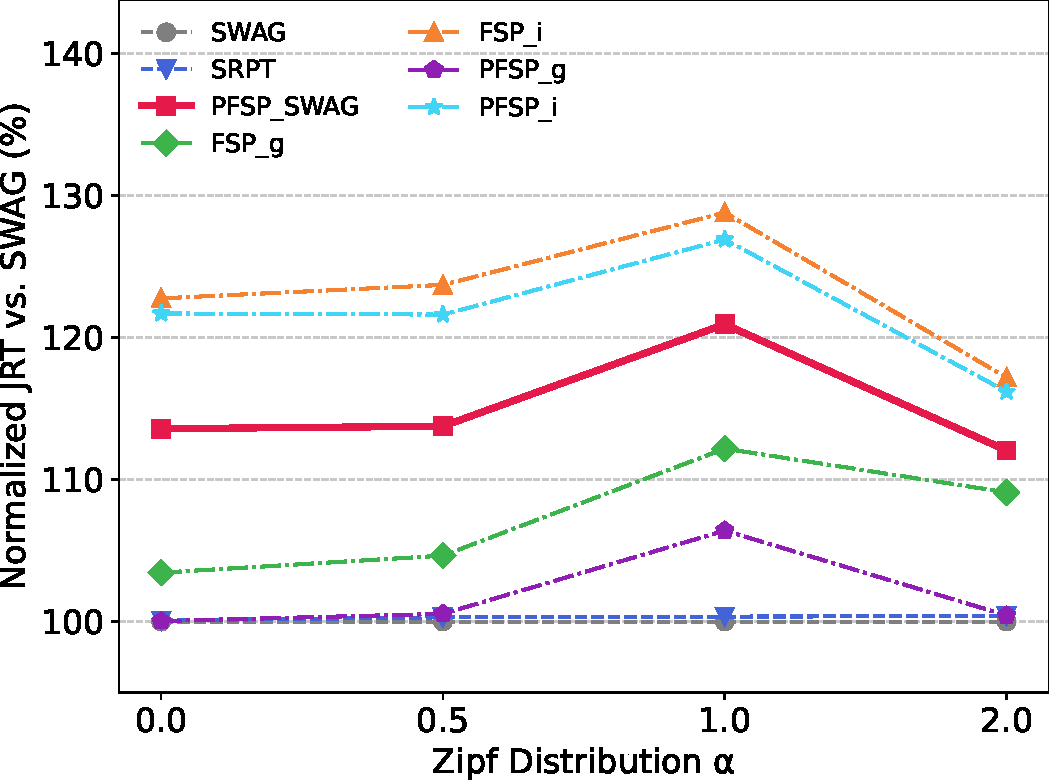
\includegraphics[width=\textwidth]{Image3/Workload_Ali2017_70_Dev=0.0.pdf}
        \caption{Utilization = 70\%}
    \end{subfigure}
    \hfill
    \begin{subfigure}[b]{0.4\textwidth}
        \centering
        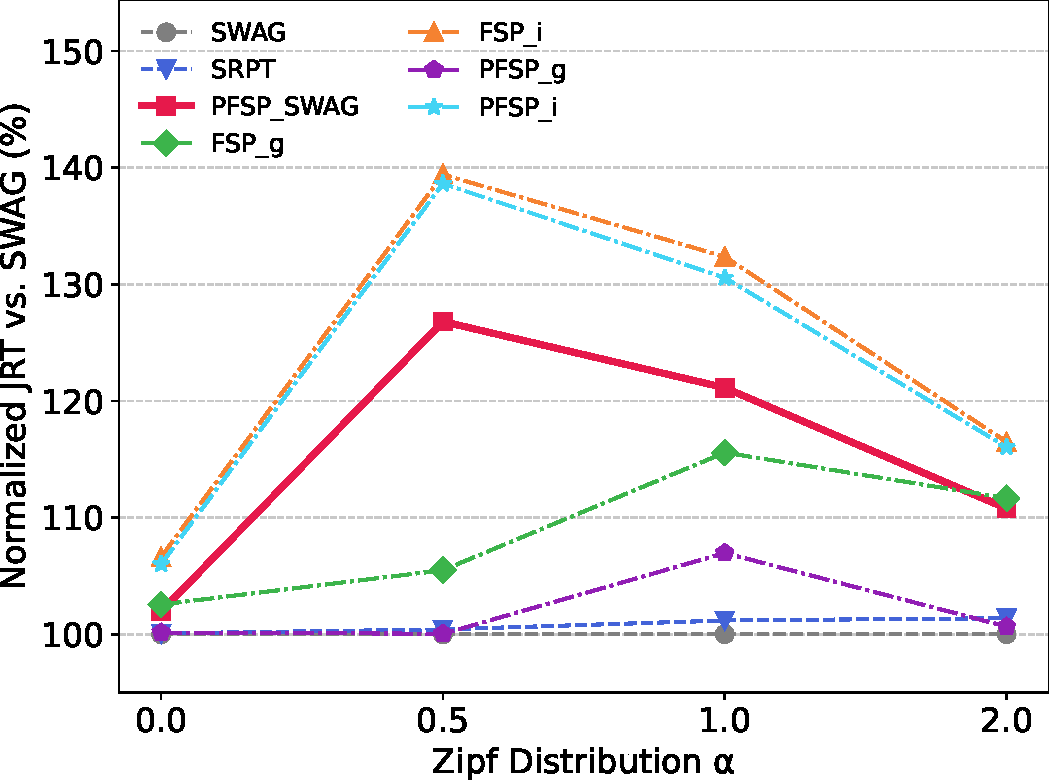
\includegraphics[width=\textwidth]{Image3/Workload_Ali2017_80_Dev=0.0.pdf}
        \caption{Utilization = 80\%}
    \end{subfigure}

    \caption{Average job response time, Alibaba 2017}
    \label{fig:JRT_Ali2017}
\end{figure*}

\begin{figure*}[t]
    \centering
    \begin{subfigure}[b]{0.4\textwidth}
        \centering
        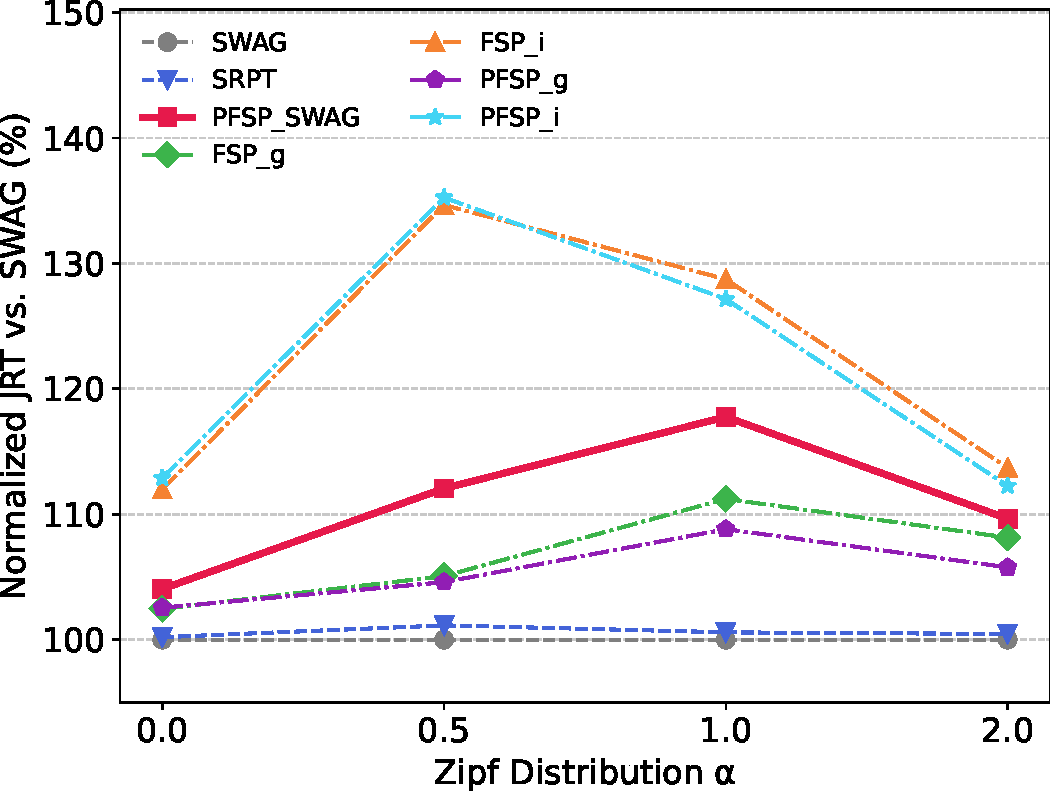
\includegraphics[width=\textwidth]{Image3/Workload_Ali2018_4_50_Dev=0.000.pdf}
        \caption{Utilization = 50\%}
    \end{subfigure}
    \hfill
    \begin{subfigure}[b]{0.4\textwidth}
        \centering
        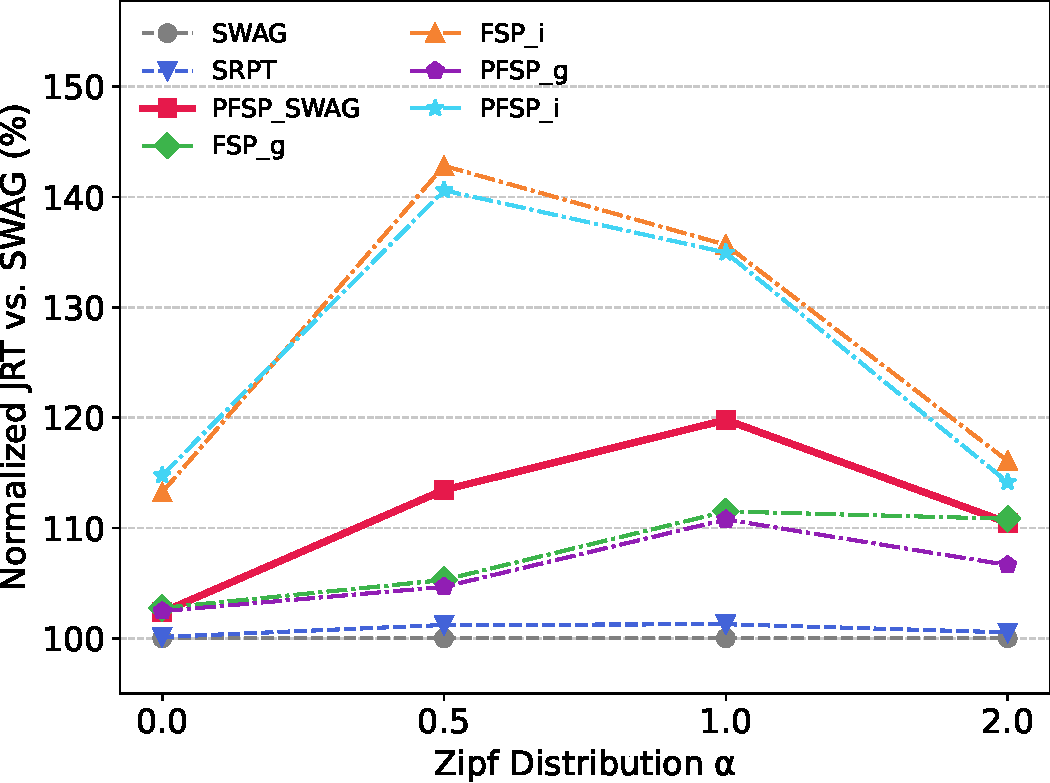
\includegraphics[width=\textwidth]{Image3/Workload_Ali2018_4_60_Dev=0.000.pdf}
        \caption{Utilization = 60\%}
    \end{subfigure}
    \vspace{0.8em}
    \begin{subfigure}[b]{0.4\textwidth}
        \centering
        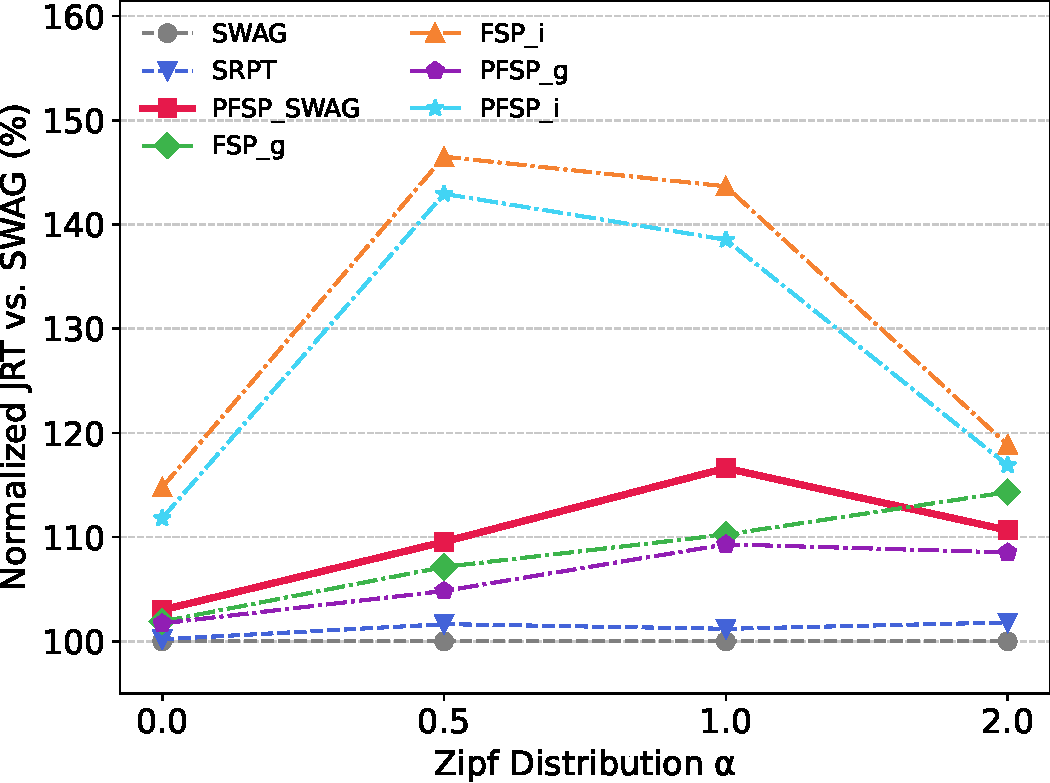
\includegraphics[width=\textwidth]{Image3/Workload_Ali2018_4_70_Dev=0.000.pdf}
        \caption{Utilization = 70\%}
    \end{subfigure}
    \hfill
    \begin{subfigure}[b]{0.4\textwidth}
        \centering
        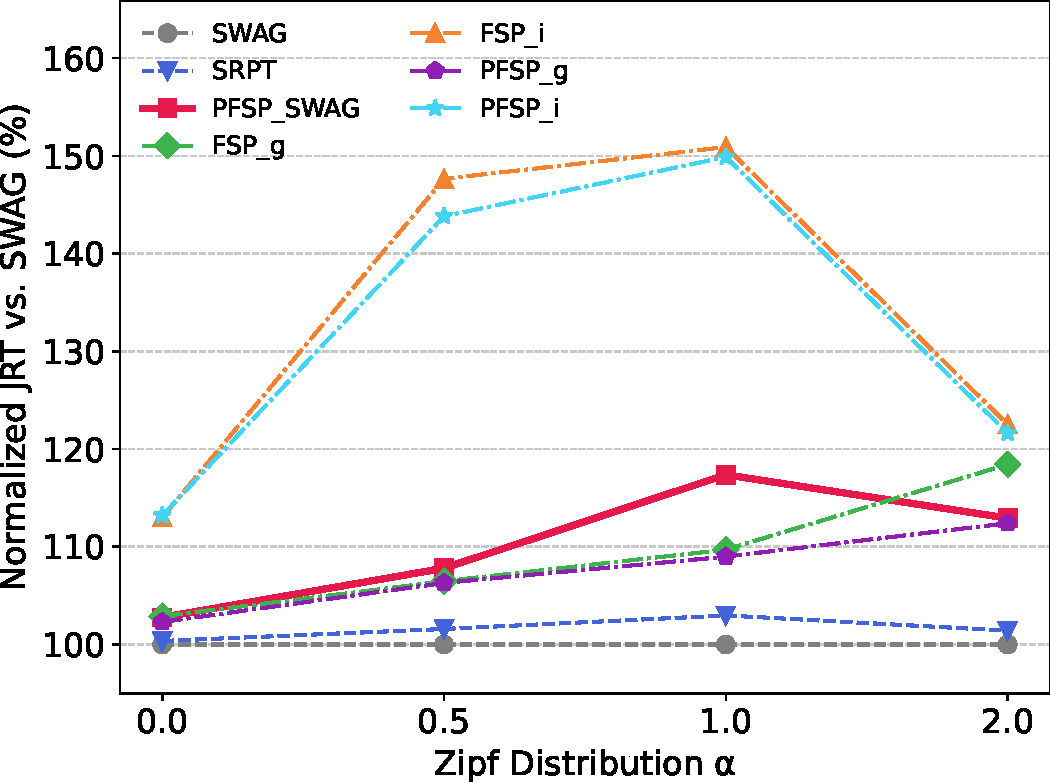
\includegraphics[width=\textwidth]{Image3/Workload_Ali2018_4_80_Dev=0.000.pdf}
        \caption{Utilization = 80\%}
    \end{subfigure}

    \caption{Average job response time, Alibaba 2018}
    \label{fig:JRT_Ali2018}
\end{figure*}

We use the average job response time and the number of jobs violating PS deadlines as the performance metrics to evaluate the dual objectives of efficiency and fairness under different scheduling policies, system utilizations and load distributions. The average job response time is defined as the average time span from each job's arrival to its completion, where a lower average job response time indicates higher job processing efficiency of the policy. The number of jobs violating PS deadlines is defined as the number of jobs whose actual completion time are later than their global PS completion times, which indicates the degree of long-term fairness in the system. A larger number of violations means that more jobs fail to finish before their completion times under the distributed PS policy, indicating a higher degree of unfairness/starvation in job scheduling. Because some of the policies have similar performance trends, we only present the results of SWAG, SRPT (efficiency-targeted policies), PFSP\_g, FSP\_g (policies based on the $GS$ scheme), PFSP\_i, FSP\_i (policies based on the $IS$ scheme) and PFSP\_SWAG (derived from the PFSP\_x framework).

Figures \ref{fig:JRT_Ali2017} and \ref{fig:JRT_Ali2018} present the average job response time of different scheduling policies under various system settings. To facilitate comparison, we set the optimal average job response time derived from SWAG policy as the $100\%$ baseline and compute the average job response time of other policies as a percentage of it. The results demonstrate that scheduling policies that are efficiency-targeted (SWAG and SRPT) or adopt the $GS$ scheme (PFSP\_g, FSP\_g) achieve better average job response times compared to those adopting the $IS$ scheme. In particular, PFSP\_g achieves fairly close performance to the SWAG policy, demonstrating its potential in balancing the trade-off between efficiency and long-term fairness. In contrast, policies that adopt the $IS$ scheme (PFSP\_i, FSP\_i, PFSP\_SWAG) guarantee strict protectiveness at the expense of worse average job response times, with the performance gap reaching up to approximately 50\%. Our proposed PFSP\_SWAG algorithm demonstrates the best average job response time among the three policies based on the $IS$ scheme, and under certain system configurations when the load distributions of jobs are highly skewed (i.e., $\alpha=2.0$), it can even outperforms the FSP\_g policy based on the $GS$ scheme.

\begin{table}[htbp]
    \centering
    \caption{Number of jobs violating PS deadlines, Alibaba 2017}
    \label{tab:count_PS_violation_Ali2017}
    \begin{tabular}{cc cccc}
        \toprule
        \multirow{2}{*}{Utilization} & \multirow{2}{*}{$\alpha$} & \multicolumn{4}{c}{Strategies} \\
        \cmidrule(lr){3-6}
        & & SWAG & SRPT & PFSP\_g & FSP\_g \\
        \midrule
        \multirow{4}{*}{$50\%$} 
        & $0.0$ & 44 & 50 & 0 & 0 \\
        & $0.5$ & 50 & 68 & 0 & 0 \\
        & $1.0$ & 50 & 68 & 0 & 0 \\
        & $2.0$ & 37 & 53 & 0 & 0 \\
        \midrule
        \multirow{4}{*}{$60\%$} 
        & $0.0$ & 41 & 46 & 0 & 0 \\
        & $0.5$ & 43 & 57 & 1 & 0 \\
        & $1.0$ & 34 & 46 & 0 & 0 \\
        & $2.0$ & 25 & 31 & 0 & 0 \\
        \midrule
        \multirow{4}{*}{$70\%$} 
        & $0.0$ & 36 & 41 & 0 & 0 \\
        & $0.5$ & 33 & 40 & 2 & 2 \\
        & $1.0$ & 23 & 28 & 0 & 0 \\
        & $2.0$ & 14 & 21 & 1 & 0 \\
        \midrule
        \multirow{4}{*}{$80\%$} 
        & $0.0$ & 29 & 32 & 1 & 1 \\
        & $0.5$ & 20 & 19 & 0 & 0 \\
        & $1.0$ & 15 & 20 & 0 & 0 \\
        & $2.0$ & 12 & 22 & 0 & 0 \\
        \bottomrule
    \end{tabular}
\end{table}

\begin{table}[htbp]
    \centering
    \caption{Number of jobs violating PS deadlines, Alibaba 2018}
    \label{tab:count_PS_violation_Ali2018}
    \begin{tabular}{cc cccc}
        \toprule
        \multirow{2}{*}{Utilization} & \multirow{2}{*}{$\alpha$} & \multicolumn{4}{c}{Strategies} \\
        \cmidrule(lr){3-6}
        & & SWAG & SRPT & PFSP\_g & FSP\_g \\
        \midrule
        \multirow{4}{*}{$50\%$} 
        & $0.0$ & 37 & 50 & 0 & 0 \\
        & $0.5$ & 57 & 64 & 1 & 0 \\
        & $1.0$ & 41 & 47 & 0 & 0 \\
        & $2.0$ & 23 & 36 & 0 & 0 \\
        \midrule
        \multirow{4}{*}{$60\%$} 
        & $0.0$ & 26 & 38 & 1 & 1 \\
        & $0.5$ & 40 & 46 & 0 & 0 \\
        & $1.0$ & 28 & 28 & 0 & 0 \\
        & $2.0$ & 17 & 26 & 0 & 0 \\
        \midrule
        \multirow{4}{*}{$70\%$} 
        & $0.0$ & 17 & 31 & 2 & 2 \\
        & $0.5$ & 32 & 41 & 0 & 0 \\
        & $1.0$ & 23 & 25 & 0 & 0 \\
        & $2.0$ & 14 & 23 & 0 & 0 \\
        \midrule
        \multirow{4}{*}{$80\%$} 
        & $0.0$ & 13 & 25 & 1 & 1 \\
        & $0.5$ & 32 & 41 & 0 & 0 \\
        & $1.0$ & 18 & 18 & 0 & 0 \\
        & $2.0$ & 12 & 18 & 0 & 0 \\
        \bottomrule
    \end{tabular}
\end{table}

Tables \ref{tab:count_PS_violation_Ali2017} and \ref{tab:count_PS_violation_Ali2018} present the number of violations to the PS deadline under different scheduling policies. We omit the $IS$ policies (including PFSP\_SWAG) from the tables because they guarantee zero violations under all conditions. The results show that both SWAG and SRPT have tens of violations in general, indicating that efficiency-targeted policies do not guarantee protectiveness in the distributed job execution case. In contrast, policies based on the $GS$ scheme have much fewer violations (zero violations in most cases). In particulr, PFSP\_g significantly decreases the number of violations while keeping a close average job response time to SWAG and SRPT at all system settings, demonstrating that it achieves a good trade-off between efficiency and long-term fairness. Meanwhile, PFSP\_SWAG guarantees zero violations while effectively decreasing the average job response time compared to other policies based on the $IS$ scheme. These empirical results suggest that the PFSP\_g and PFSP\_SWAG can be selectively applied to different scenarios depending on the system's specific trade-offs between fairness and efficiency.

\subsection{On Inaccurate Job Load Estimation}

All scheduling policies introduced above rely on accurate estimations of job load distributions across sites. Inaccurate estimations can lead to system performance degradation in both average job response time and PS deadline violations. To evaluate the impact of inaccurate estimations, we randomly generate the job load estimates following a uniform distribution between $-x$ and $x$, where $x$ is the maximum deviation assumed. Based on our evaluation with 10,000 jobs, when the estimated job loads uniformly deviate within $\pm10\%$ of the ground truth (i.e., ranging from $90\%$ to $110\%$), the number of jobs violating PS deadlines rises up to hundreds across different scheduling policies. Estimation errors manifest in two distinct forms:

\begin{itemize}[leftmargin=*]
    \item \textbf{Over-estimation} gives a larger estimated load of a job than its actual load, which may deprioritize it in the execution order. In this case, other jobs in the system can either have their execution order advanced or kept unchanged, so generally their completion times will not degrade and the number of jobs violating PS deadlines will increase by one at most. Consequently, over-estimation predominantly impacts the over-estimated job itself, degrading its own completion time.%  potentially leading to earlier completion times.    However, because other concurrently running jobs will either have higher priorities or keep the priorities unchanged, their completion times generally remain within their PS deadlines. 
    
    \item \textbf{Under-estimation} gives a smaller estimated load of a job than its actual load. As a result, an under-estimated job is not completed and needs to continue execution even when its (estimated) real load drops to 0. This introduces severe systemic risks because with its (estimated) real load being 0, it will be prioritized for execution by all scheduling policies (including efficiency-targeted ones and those based on the GS and IS schemes), inducing serious head-of-line blocking and starving subsequent jobs, which ultimately triggers a surge of PS deadline violations.
\end{itemize}

To counteract performance degradation under job load under-estimations, we propose a mitigation mechanism, called Processor Sharing Fallback (PSF). PSF allocates a fair capacity share to these under-estimated jobs: Once a job has its (estimated) real load drop to 0 at a site but has not completed execution at this site, it transitions into a fallback PS state. In this state, the job is assigned a fixed equal share ($1/N_{\text{active}}$) of the site capacity, where $N_{\text{active}}$ represents the concurrent count of active jobs with remaining real load at the site. The leftover capacity of the site is then used to schedule non-fallback jobs following the original scheduling policy. Note that the PSF mechanism will be activated only when a job's load is underestimated. Consequently, it can be seamlessly integrated as a lightweight add-on module to existing scheduling policies, incurring negligible overhead when load estimations are accurate.%Note that the PSF mechanism will only be triggered if a job has its load under-estimated, thus it can be deployed as an add-on mechanism with little overhead when the system has accurate load estimation.
%This indicates that the PSF mechanism effectively mitigates the performance degradation caused by under-estimation of job loads. %The results show that the PSF mechanism effectively mitigates the performance degradation caused by under-estimation of job loads, especially for efficiency-targeted policies (SWAG and SRPT) and policies based on the $GS$ scheme (PFSP\_g and FSP\_g). With the PSF mechanism, these policies can achieve average job response times close to their counterparts with accurate job load estimations, while significantly reducing the number of PS deadline violations.


\begin{table}[ht]
\centering
\caption{Number of jobs violating PS deadlines with/without PSF, 10\% deviation, 70\% utilization, Alibaba 2017}
\label{tab:PSF_ali17_1}
\resizebox{\textwidth}{!}{\begin{tabular}{l cccc c cccc}
\toprule
& \multicolumn{4}{c}{\textbf{Without PSF}} & & \multicolumn{4}{c}{\textbf{With PSF}} \\
\cmidrule{2-5} \cmidrule{7-10}
\textbf{Policy} & $\alpha=0.0$ & $\alpha=0.5$ & $\alpha=1.0$ & $\alpha=2.0$ & & $\alpha=0.0$ & $\alpha=0.5$ & $\alpha=1.0$ & $\alpha=2.0$ \\
\midrule
SWAG & 173  & 300 & 357 & 732 & & 69 & 91 & 97 & 160 \\
SRPT & 182 & 322 & 369 & 768 & & 82 & 102 & 102 & 164 \\
PFSP\_g & 217 & 195 & 363 & 577 & & 48 & 52 & 57 & 109 \\
FSP\_g & 104 & 83 & 79 & 52 & & 29 & 48 & 53 & 110 \\
PFSP\_SWAG & 543 & 973 & 909 & 888 & & 70 & 74 & 65 & 72 \\
PFSP\_i & 774 & 1232 & 978 & 981 & &  79 & 80 & 62 & 72 \\
FSP\_i & 285 & 547 & 513 & 480 & & 71 & 71 & 58 & 67 \\
\bottomrule
\end{tabular}}
\end{table}

\begin{table}[ht]
\centering
\caption{Number of jobs violating PS deadlines with/without PSF, 20\% deviation, 70\% utilization, Alibaba 2017}
\label{tab:PSF_ali17_2}
\resizebox{\textwidth}{!}{
\begin{tabular}{l cccc c cccc}
\toprule
& \multicolumn{4}{c}{\textbf{Without PSF}} & & \multicolumn{4}{c}{\textbf{With PSF}} \\
\cmidrule{2-5} \cmidrule{7-10}
\textbf{Policy} & $\alpha=0.0$ & $\alpha=0.5$ & $\alpha=1.0$ & $\alpha=2.0$ & & $\alpha=0.0$ & $\alpha=0.5$ & $\alpha=1.0$ & $\alpha=2.0$ \\
\midrule
SWAG & 443  & 366 & 556 & 1185 & & 97 & 135 & 136 & 214 \\
SRPT & 451 & 372 & 552 & 1149 & & 108 & 133 & 135 & 226 \\
PFSP\_g & 395 & 371 & 521 & 791 & & 80 & 113 & 110 & 172 \\
FSP\_g & 245 & 167 & 197 & 184 & & 78 & 106 & 105 & 167 \\
PFSP\_SWAG & 970 & 1509 & 1606 & 1519 & & 97 & 143 & 98 & 107 \\
PFSP\_i & 1314 & 1976 & 1623 & 1662 & & 109 & 147 & 102 & 106 \\
FSP\_i & 439 & 920 & 1039 & 1000 & & 98 & 147 & 98 & 94 \\
\bottomrule
\end{tabular}}
\end{table}

\begin{table}[ht]
\centering
\caption{Number of jobs violating PS deadlines with/without PSF, 30\% deviation, 70\% utilization, Alibaba 2017}
\label{tab:PSF_ali17_3}
\resizebox{\textwidth}{!}{
\begin{tabular}{l cccc c cccc}
\toprule
& \multicolumn{4}{c}{\textbf{Without PSF}} & & \multicolumn{4}{c}{\textbf{With PSF}} \\
\cmidrule{2-5} \cmidrule{7-10}
\textbf{Policy} & $\alpha=0.0$ & $\alpha=0.5$ & $\alpha=1.0$ & $\alpha=2.0$ & & $\alpha=0.0$ & $\alpha=0.5$ & $\alpha=1.0$ & $\alpha=2.0$ \\
\midrule
SWAG & 369  & 607 & 896 & 1495 & & 106 & 146 & 178 & 184 \\
SRPT & 363 & 666 & 889 & 1526 & & 108 & 143 & 780 & 182 \\
PFSP\_g & 317 & 561 & 580 & 1476 & & 84 & 105 & 118 & 162 \\
FSP\_g & 132 & 191 & 169 & 547 & & 84 & 98 & 112 & 161 \\
PFSP\_SWAG & 632 & 1499 & 1486 & 2157 & & 114 & 130 & 134 & 154 \\
PFSP\_i & 697 & 1721 & 1466 & 2421 & &  125 & 136 & 126 & 146 \\
FSP\_i & 293 & 872 & 740 & 1465 & & 116 & 131 & 120 & 142 \\
\bottomrule
\end{tabular}}
\end{table}

\begin{table}[ht]
\centering
\caption{Number of jobs violating PS deadlines with/without PSF, 40\% deviation, 70\% utilization, Alibaba 2017}
\label{tab:PSF_ali17_4}
\resizebox{\textwidth}{!}{
\begin{tabular}{l cccc c cccc}
\toprule
& \multicolumn{4}{c}{\textbf{Without PSF}} & & \multicolumn{4}{c}{\textbf{With PSF}} \\
\cmidrule{2-5} \cmidrule{7-10}
\textbf{Policy} & $\alpha=0.0$ & $\alpha=0.5$ & $\alpha=1.0$ & $\alpha=2.0$ & & $\alpha=0.0$ & $\alpha=0.5$ & $\alpha=1.0$ & $\alpha=2.0$ \\
\midrule
SWAG & 1143  & 1351 & 1925 & 2826 & & 140 & 282 & 306 & 352 \\
SRPT & 1147 & 1518 & 1920 & 2819 & & 141 & 260 & 327 & 326 \\
PFSP\_g & 1060 & 1304 & 1488 & 2631 & & 120 & 245 & 215 & 296 \\
FSP\_g & 354 & 548 & 597 & 1572 & & 111 & 248 & 205 & 301 \\
PFSP\_SWAG & 1640 & 2353 & 3338 & 3375 & & 149 & 199 & 215 & 247 \\
PFSP\_i & 1903 & 2911 & 3648 & 3765 & &  159 & 205 & 237 & 248 \\
FSP\_i & 748 & 1438 & 2391 & 2582 & & 144 & 199 & 222 & 249 \\
\bottomrule
\end{tabular}}
\end{table}

\begin{table}[ht]
\centering
\caption{Number of jobs violating PS deadlines with/without PSF, 10\% deviation, 70\% utilization, Alibaba 2018}
\label{tab:PSF_ali18_1}
\resizebox{\textwidth}{!}{\begin{tabular}{l cccc c cccc}
\toprule
& \multicolumn{4}{c}{\textbf{Without PSF}} & & \multicolumn{4}{c}{\textbf{With PSF}} \\
\cmidrule{2-5} \cmidrule{7-10}
\textbf{Policy} & $\alpha=0.0$ & $\alpha=0.5$ & $\alpha=1.0$ & $\alpha=2.0$ & & $\alpha=0.0$ & $\alpha=0.5$ & $\alpha=1.0$ & $\alpha=2.0$ \\
\midrule
SWAG & 92  & 98 & 188 & 178 & & 44 & 47 & 62 & 76 \\
SRPT & 108 & 91 & 200 & 183 & & 55 & 52 & 69 & 81 \\
PFSP\_g & 81 & 40 & 133 & 149 & & 30 & 19 & 27 & 62 \\
FSP\_g & 53 & 27 & 37 & 30 & & 29 & 20 & 25 & 65 \\
PFSP\_SWAG & 394 & 247 & 461 & 276 & & 39 & 41 & 31 & 37 \\
PFSP\_i & 423 & 350 & 513 & 307 & &  41 & 37 & 37 & 42 \\
FSP\_i & 196 & 102 & 258 & 137 & & 36 & 34 & 31 & 36 \\
\bottomrule
\end{tabular}}
\end{table}

\begin{table}[ht]
\centering
\caption{Number of jobs violating PS deadlines with/without PSF, 20\% deviation, 70\% utilization, Alibaba 2018}
\label{tab:PSF_ali18_2}
\resizebox{\textwidth}{!}{
\begin{tabular}{l cccc c cccc}
\toprule
& \multicolumn{4}{c}{\textbf{Without PSF}} & & \multicolumn{4}{c}{\textbf{With PSF}} \\
\cmidrule{2-5} \cmidrule{7-10}
\textbf{Policy} & $\alpha=0.0$ & $\alpha=0.5$ & $\alpha=1.0$ & $\alpha=2.0$ & & $\alpha=0.0$ & $\alpha=0.5$ & $\alpha=1.0$ & $\alpha=2.0$ \\
\midrule
SWAG & 145  & 209 & 425 & 398 & & 38 & 63 & 65 & 90 \\
SRPT & 163 & 209 & 394 & 408 & & 48 & 64 & 67 & 84 \\
PFSP\_g & 144 & 216 & 315 & 346 & & 34 & 33 & 45 & 70 \\
FSP\_g & 70 & 52 & 99 & 94 & & 33 & 32 & 44 & 73 \\
PFSP\_SWAG & 450 & 564 & 745 & 541 & & 45 & 55 & 53 & 51 \\
PFSP\_i & 498 & 625 & 774 & 536 & &  46 & 58 & 51 & 49 \\
FSP\_i & 185 & 293 & 355 & 281 & & 44 & 53 & 50 & 48 \\
\bottomrule
\end{tabular}}
\end{table}

\begin{table}[ht]
\centering
\caption{Number of jobs violating PS deadlines with/without PSF, 30\% deviation, 70\% utilization, Alibaba 2018}
\label{tab:PSF_ali18_3}
\resizebox{\textwidth}{!}{
\begin{tabular}{l cccc c cccc}
\toprule
& \multicolumn{4}{c}{\textbf{Without PSF}} & & \multicolumn{4}{c}{\textbf{With PSF}} \\
\cmidrule{2-5} \cmidrule{7-10}
\textbf{Policy} & $\alpha=0.0$ & $\alpha=0.5$ & $\alpha=1.0$ & $\alpha=2.0$ & & $\alpha=0.0$ & $\alpha=0.5$ & $\alpha=1.0$ & $\alpha=2.0$ \\
\midrule
SWAG & 880  & 386 & 801 & 746 & & 106 & 80 & 161 & 176 \\
SRPT & 884 & 362 & 761 & 760 & & 113 & 88 & 150 & 180 \\
PFSP\_g & 947 & 290 & 597 & 638 & & 101 & 59 & 156 & 156 \\
FSP\_g & 243 & 87 & 89 & 218 & & 99 & 56 & 153 & 165 \\
PFSP\_SWAG & 1666 & 1078 & 1785 & 946 & & 135 & 75 & 121 & 88 \\
PFSP\_i & 2009 & 1426 & 2012 & 1103 & &  140 & 80 & 131 & 93 \\
FSP\_i & 767 & 423 & 935 & 514 & & 143 & 71 & 126 & 88 \\
\bottomrule
\end{tabular}}
\end{table}

\begin{table}[ht]
\centering
\caption{Number of jobs violating PS deadlines with/without PSF, 40\% deviation, 70\% utilization, Alibaba 2018}
\label{tab:PSF_ali18_4}
\resizebox{\textwidth}{!}{
\begin{tabular}{l cccc c cccc}
\toprule
& \multicolumn{4}{c}{\textbf{Without PSF}} & & \multicolumn{4}{c}{\textbf{With PSF}} \\
\cmidrule{2-5} \cmidrule{7-10}
\textbf{Policy} & $\alpha=0.0$ & $\alpha=0.5$ & $\alpha=1.0$ & $\alpha=2.0$ & & $\alpha=0.0$ & $\alpha=0.5$ & $\alpha=1.0$ & $\alpha=2.0$ \\
\midrule
SWAG & 778  & 369 & 927 & 779 & & 134 & 123 & 199 & 151 \\
SRPT & 801 & 408 & 964 & 751 & & 142 & 127 & 198 & 152 \\
PFSP\_g & 727 & 327 & 817 & 624 & & 126 & 95 & 176 & 130 \\
FSP\_g & 446 & 191 & 386 & 263 & & 123 & 95 & 177 & 139 \\
PFSP\_SWAG & 1229 & 903 & 2053 & 940 & & 178 & 124 & 167 & 106 \\
PFSP\_i & 1325 & 1074 & 2085 & 980 & &  173 & 133 & 171 & 107 \\
FSP\_i & 779 & 507 & 1452 & 419 & & 170 & 129 & 166 & 110 \\
\bottomrule
\end{tabular}}
\end{table}


Tables \ref{tab:PSF_ali17_1} through \ref{tab:PSF_ali18_4} illustrate the impact of the PSF mechanism on PS deadline violations under different deviations of job load estimations (maximum deviation = $10\%$, $20\%$, $30\%$ and $40\%$) for both datasets. Since the performance trends for different system utilizations are similar, we present the representative results for $70\%$ system utilization only.  As can be seen, integrating the PSF mechanism significantly reduces violations for all policies, where our proposed protective scheduling policies outperform efficiency-targeted baselines in most cases, especially when the job load distributions are highly skewed. It can also be observed that policies based on the GS scheme (FSP\_g, PFSP\_g) yield the lowest violation counts. This is because these policies set the global PS completion time of a job as its deadline at all sites for scheduling purposes. The global PS completion time is given by the maximum of the site-specific PS completion times across all sites. Thus, it is less affected by under-estimation of job loads at individual sites than the site-specific PS completion times. %The results indicate that policies under the $GS$ scheme (FSP\_g, PFSP\_g) inherently yield the lowest violation counts.



\begin{figure*}[t]
    \centering
    \begin{subfigure}[b]{0.4\textwidth}
        \centering
        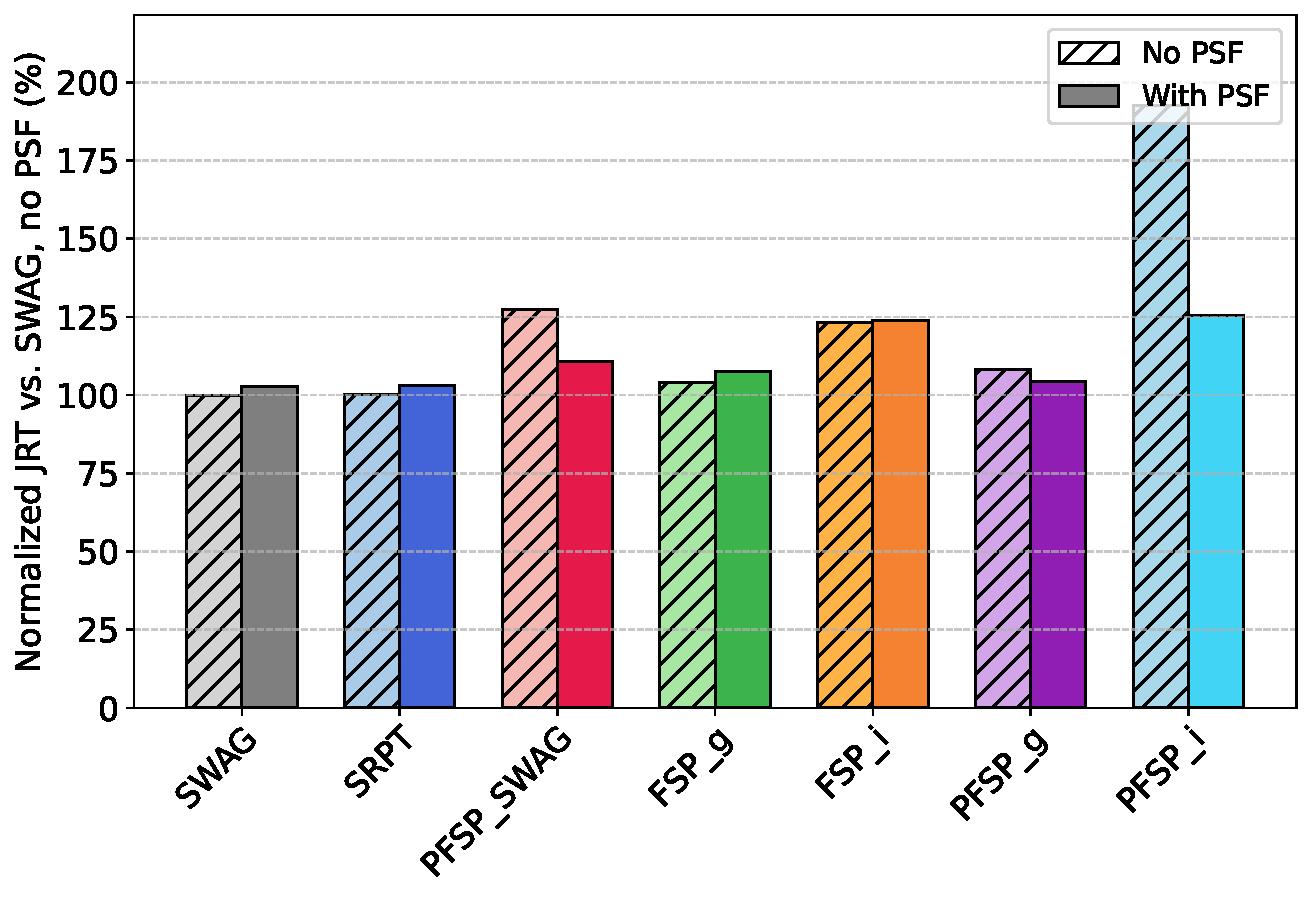
\includegraphics[width=\textwidth]{Image3/PSF_Bar_Ali2017_70_alpha=0.0_dev=0.1.pdf}
        \caption{$\alpha = 0.0$}
    \end{subfigure}
    \hfill
    \begin{subfigure}[b]{0.4\textwidth}
        \centering
        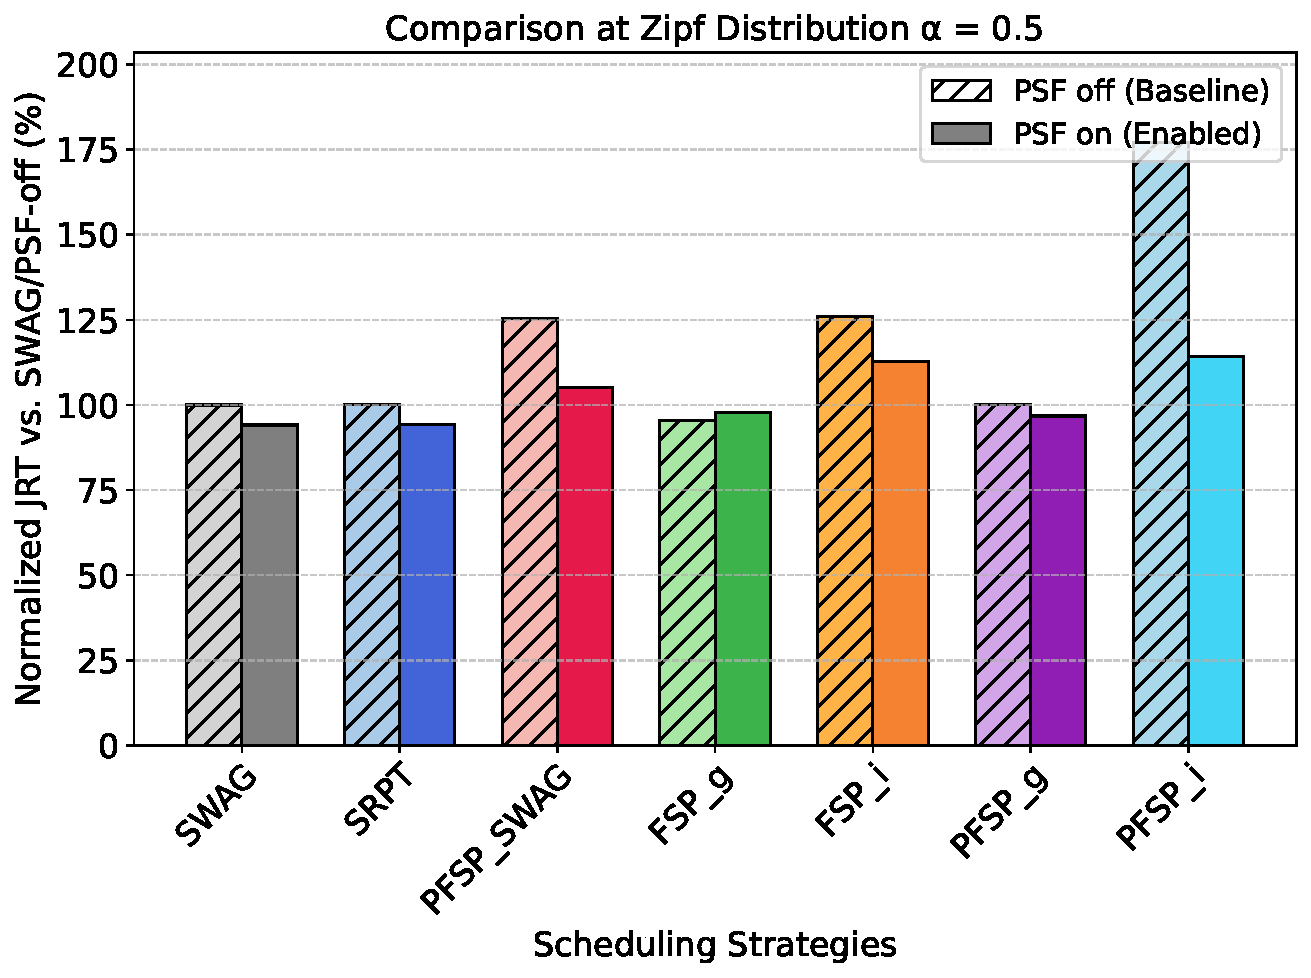
\includegraphics[width=\textwidth]{Image3/PSF_Bar_Ali2017_70_alpha=0.5_dev=0.1.pdf}
        \caption{$\alpha = 0.5$}
    \end{subfigure}
    \vspace{0.8em}
    \begin{subfigure}[b]{0.4\textwidth}
        \centering
        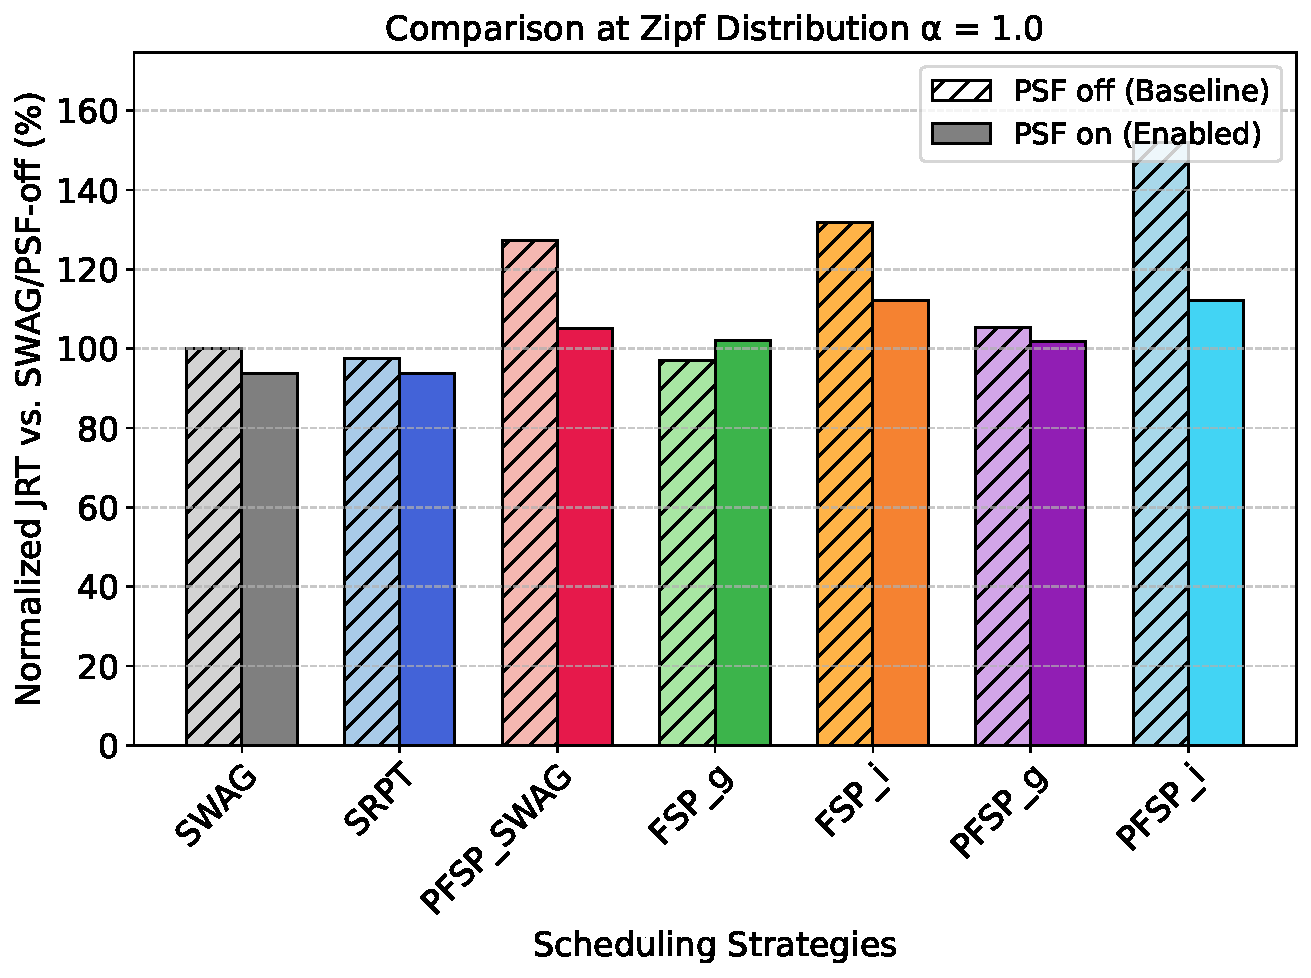
\includegraphics[width=\textwidth]{Image3/PSF_Bar_Ali2017_70_alpha=1.0_dev=0.1.pdf}
        \caption{$\alpha = 1.0$}
    \end{subfigure}
    \hfill
    \begin{subfigure}[b]{0.4\textwidth}
        \centering
        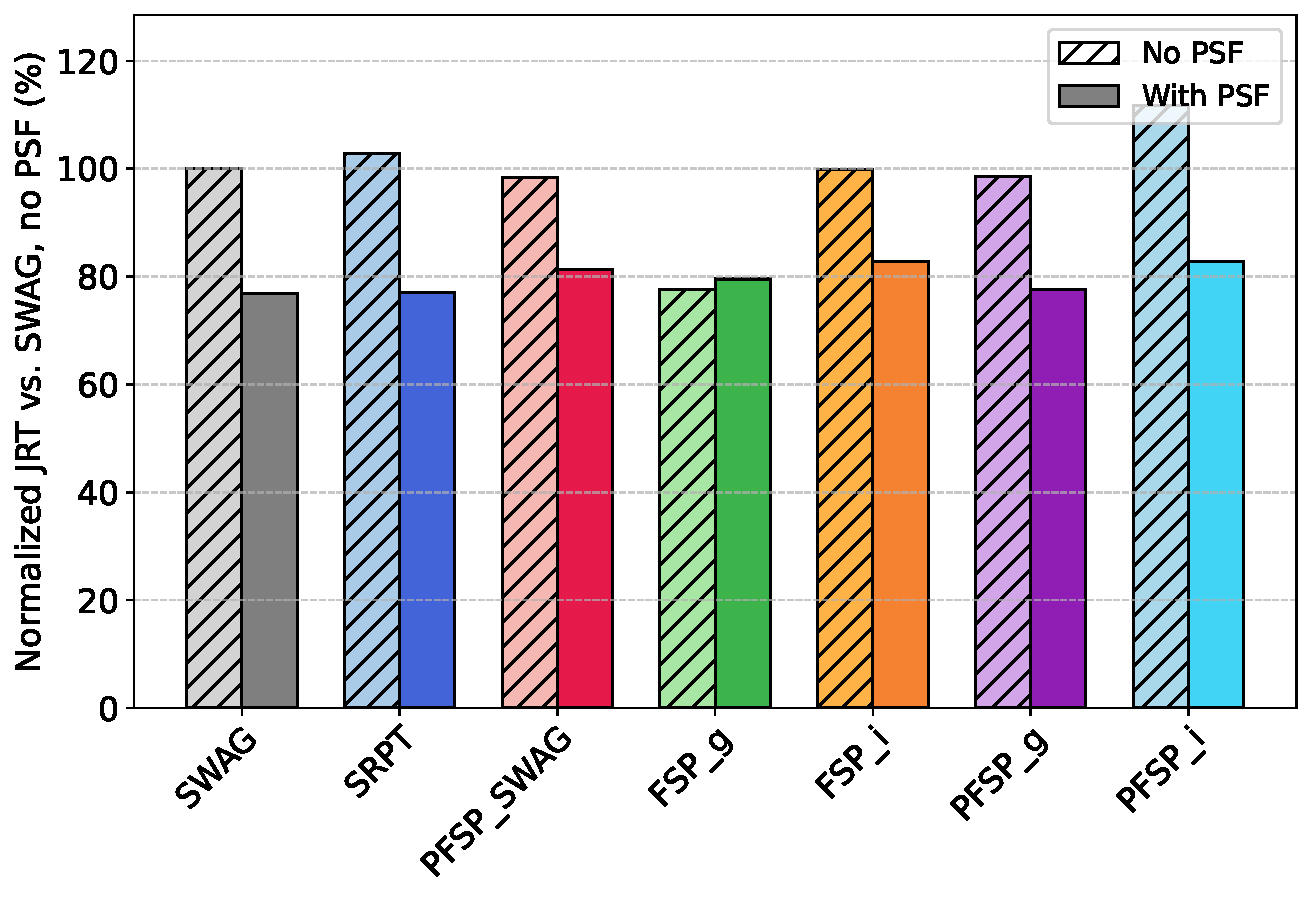
\includegraphics[width=\textwidth]{Image3/PSF_Bar_Ali2017_70_alpha=2.0_dev=0.1.pdf}
        \caption{$\alpha = 2.0$}
    \end{subfigure}

    \caption{Average job response time with/without PSF, 10\% deviation, 70\% utilization, Alibaba 2017}
    \label{fig:JRT_Ali2017_err=0.1}
\end{figure*}

\begin{figure*}[t]
    \centering
    \begin{subfigure}[b]{0.4\textwidth}
        \centering
        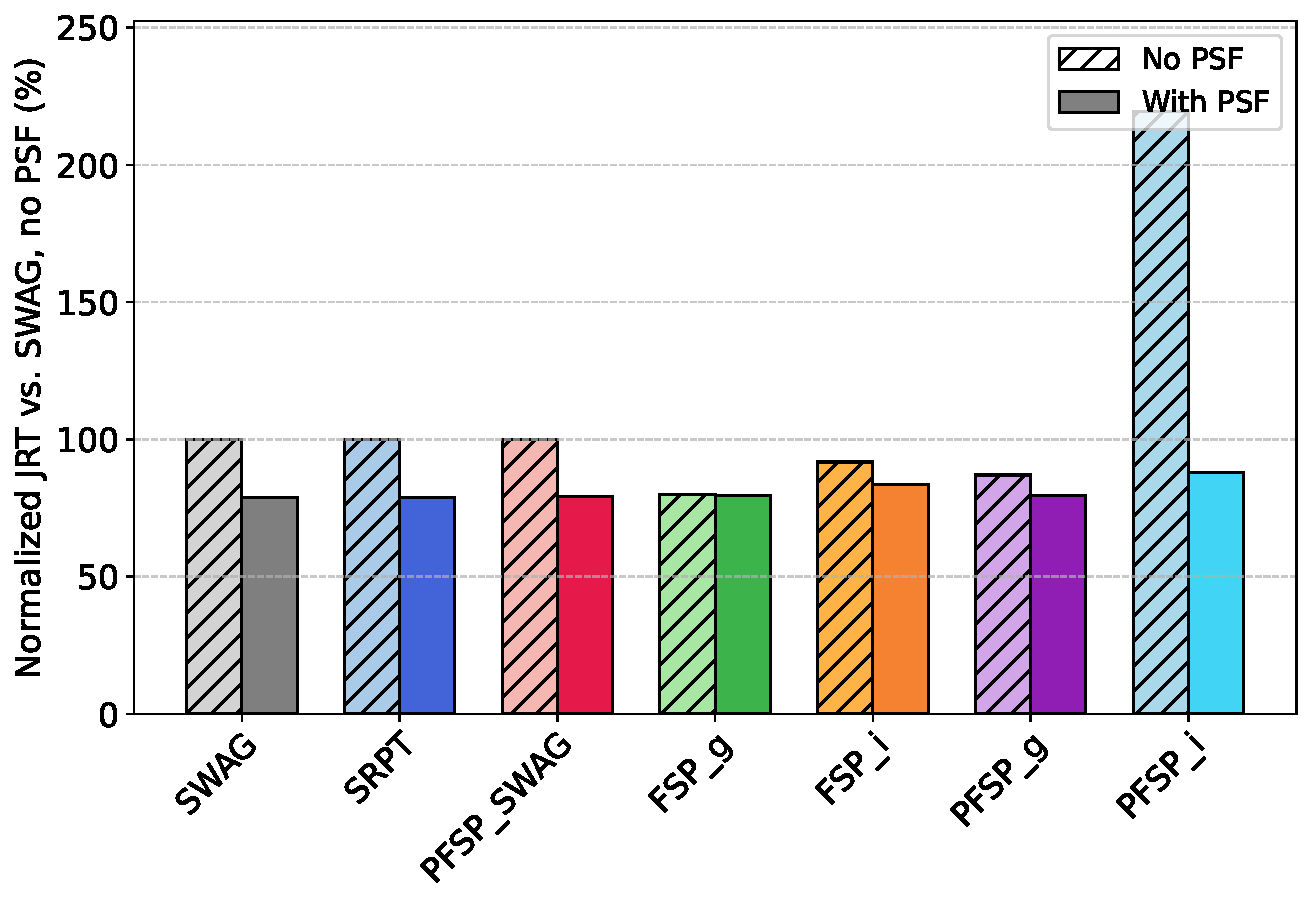
\includegraphics[width=\textwidth]{Image3/PSF_Bar_Ali2017_70_alpha=0.0_dev=0.2.pdf}
        \caption{$\alpha = 0.0$}
    \end{subfigure}
    \hfill
    \begin{subfigure}[b]{0.4\textwidth}
        \centering
        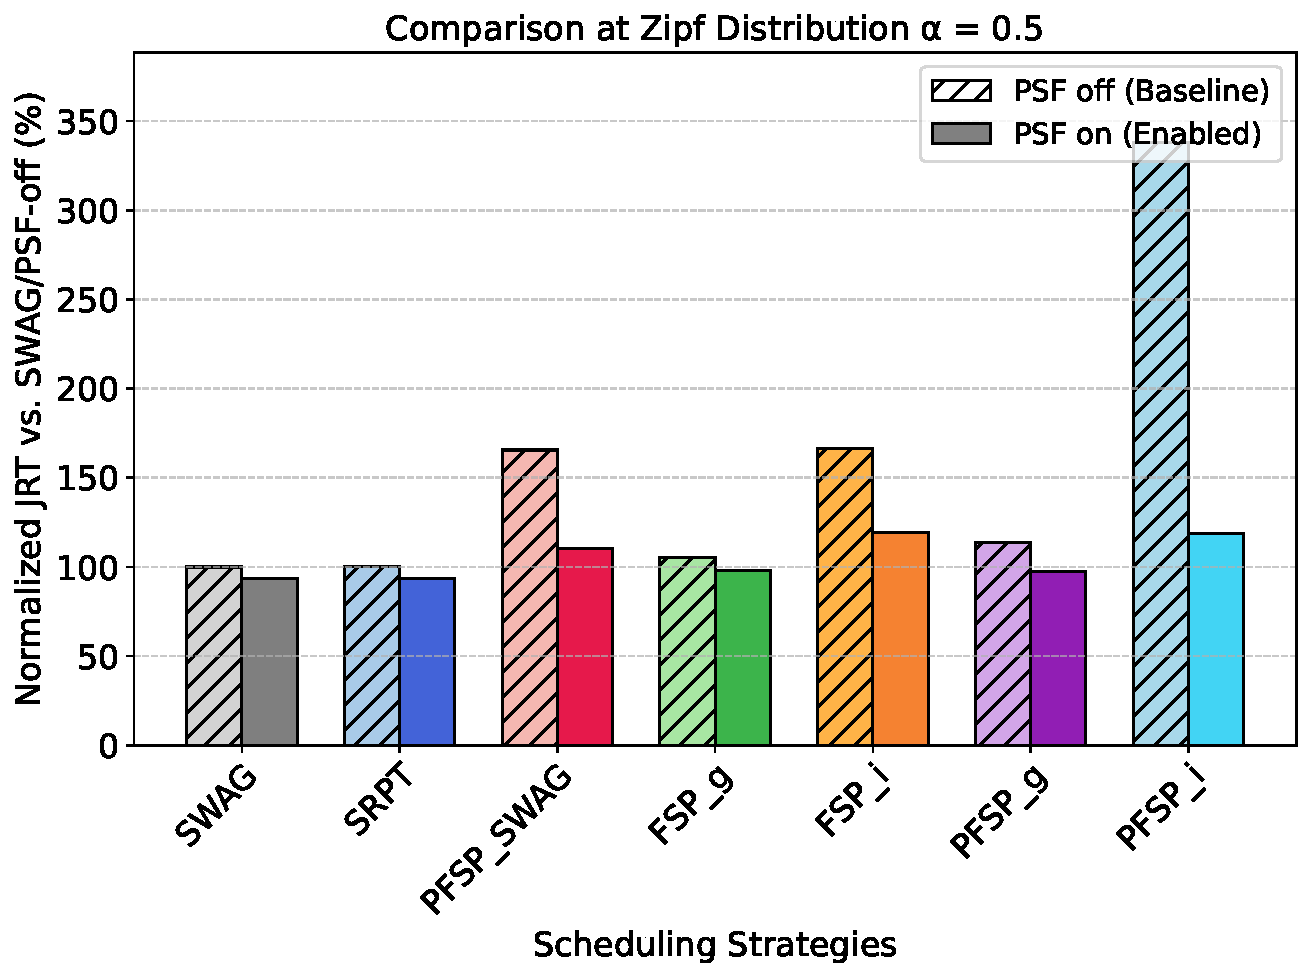
\includegraphics[width=\textwidth]{Image3/PSF_Bar_Ali2017_70_alpha=0.5_dev=0.2.pdf}
        \caption{$\alpha = 0.5$}
    \end{subfigure}
    \vspace{0.8em}
    \begin{subfigure}[b]{0.4\textwidth}
        \centering
        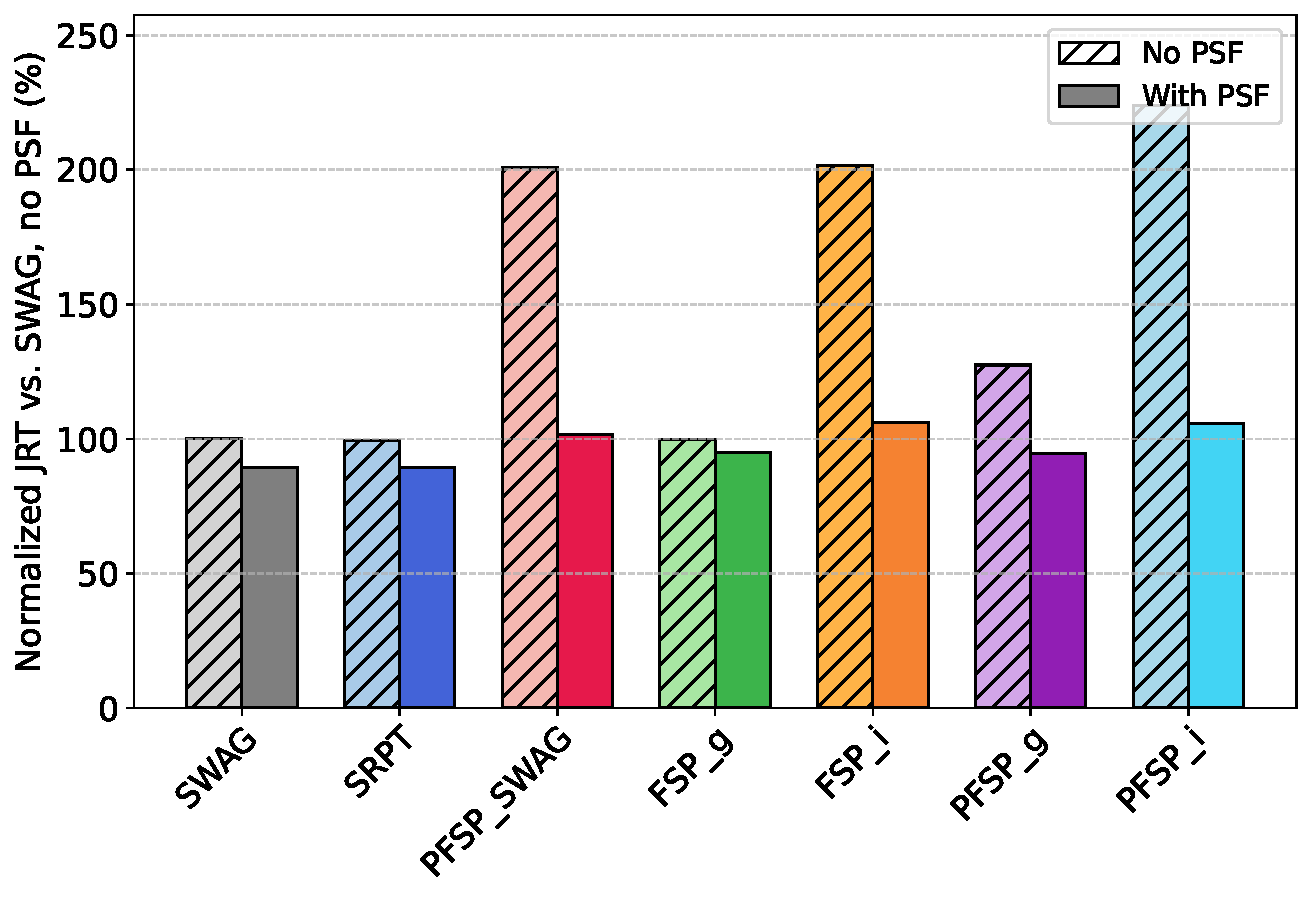
\includegraphics[width=\textwidth]{Image3/PSF_Bar_Ali2017_70_alpha=1.0_dev=0.2.pdf}
        \caption{$\alpha = 1.0$}
    \end{subfigure}
    \hfill
    \begin{subfigure}[b]{0.4\textwidth}
        \centering
        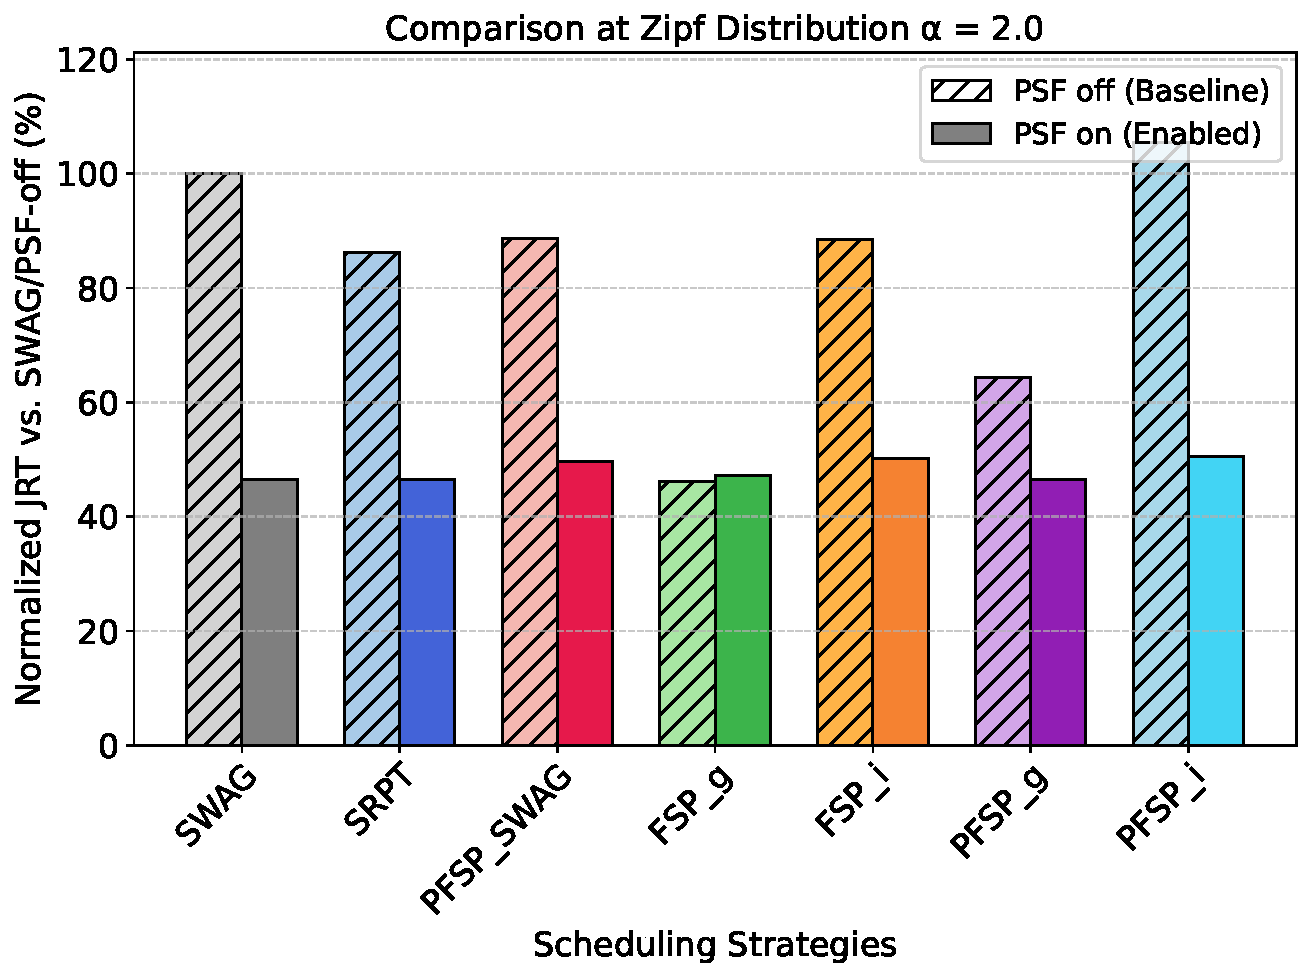
\includegraphics[width=\textwidth]{Image3/PSF_Bar_Ali2017_70_alpha=2.0_dev=0.2.pdf}
        \caption{$\alpha = 2.0$}
    \end{subfigure}

    \caption{Average job response time with/without PSF, 20\% deviation, 70\% utilization, Alibaba 2017}
    \label{fig:JRT_Ali2017_err=0.2}
\end{figure*}

\begin{figure*}[t]
    \centering
    \begin{subfigure}[b]{0.4\textwidth}
        \centering
        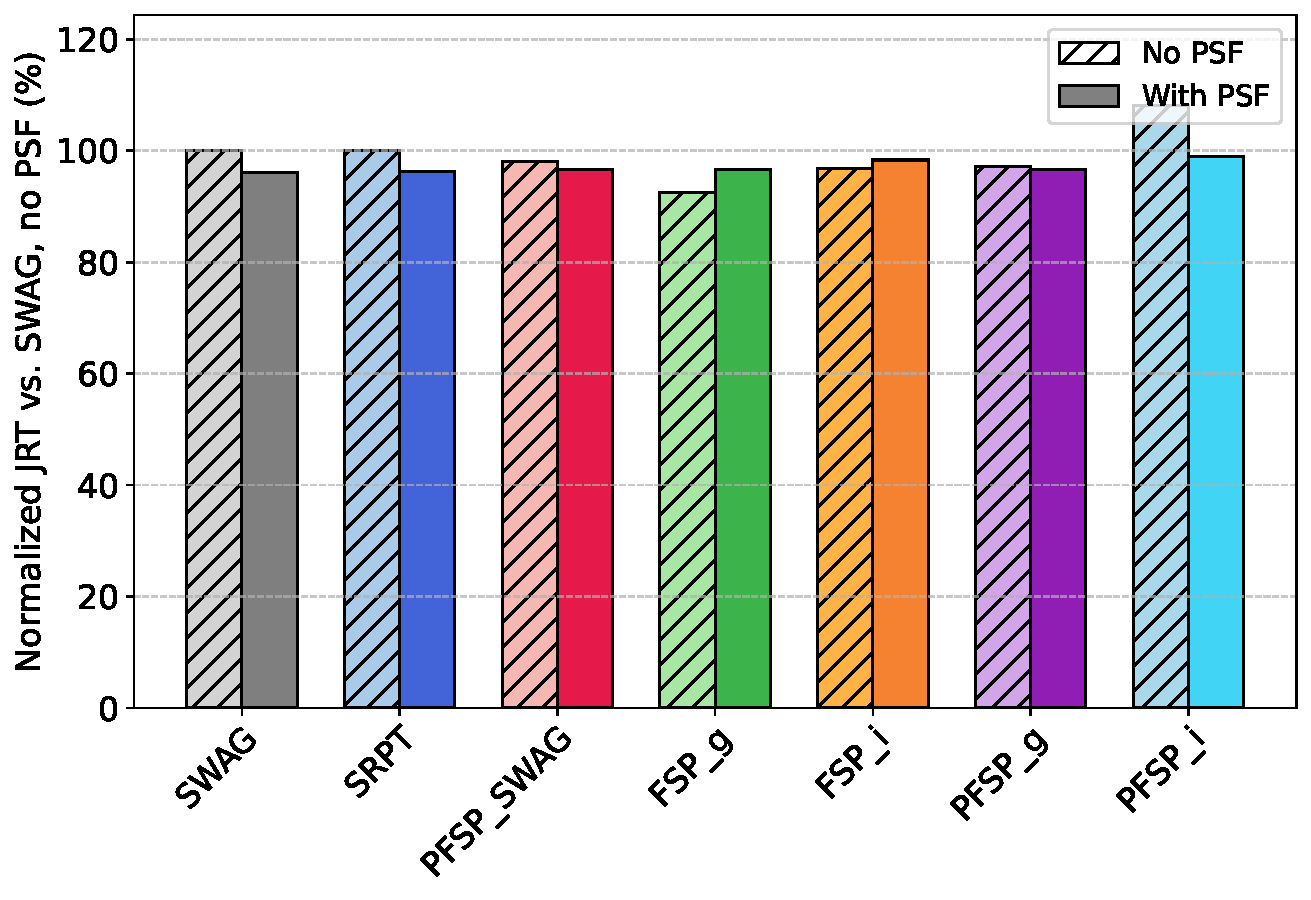
\includegraphics[width=\textwidth]{Image3/PSF_Bar_Ali2017_70_alpha=0.0_dev=0.3.pdf}
        \caption{$\alpha = 0.0$}
    \end{subfigure}
    \hfill
    \begin{subfigure}[b]{0.4\textwidth}
        \centering
        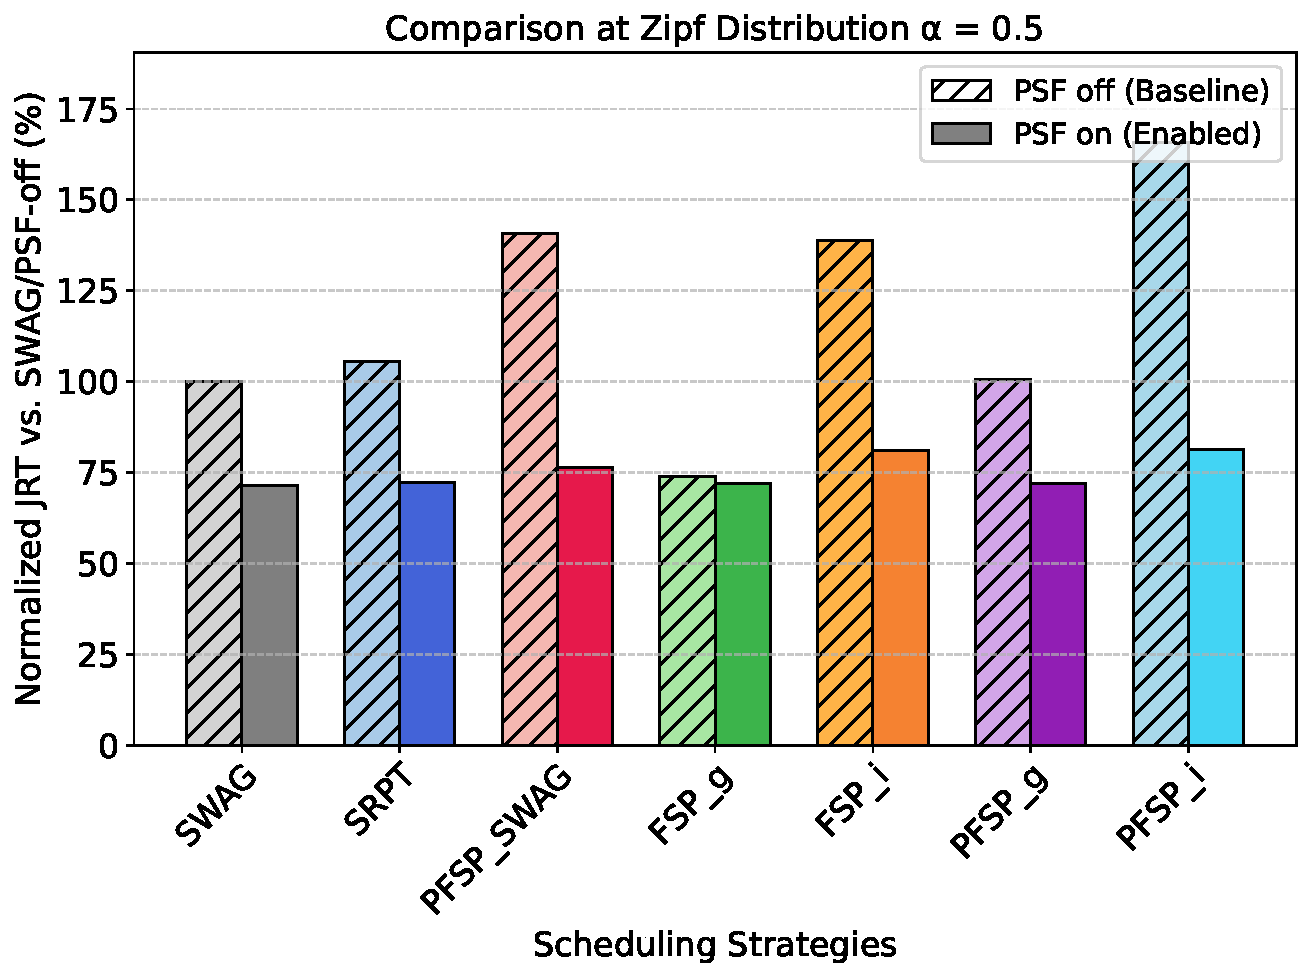
\includegraphics[width=\textwidth]{Image3/PSF_Bar_Ali2017_70_alpha=0.5_dev=0.3.pdf}
        \caption{$\alpha = 0.5$}
    \end{subfigure}
    \vspace{0.8em}
    \begin{subfigure}[b]{0.4\textwidth}
        \centering
        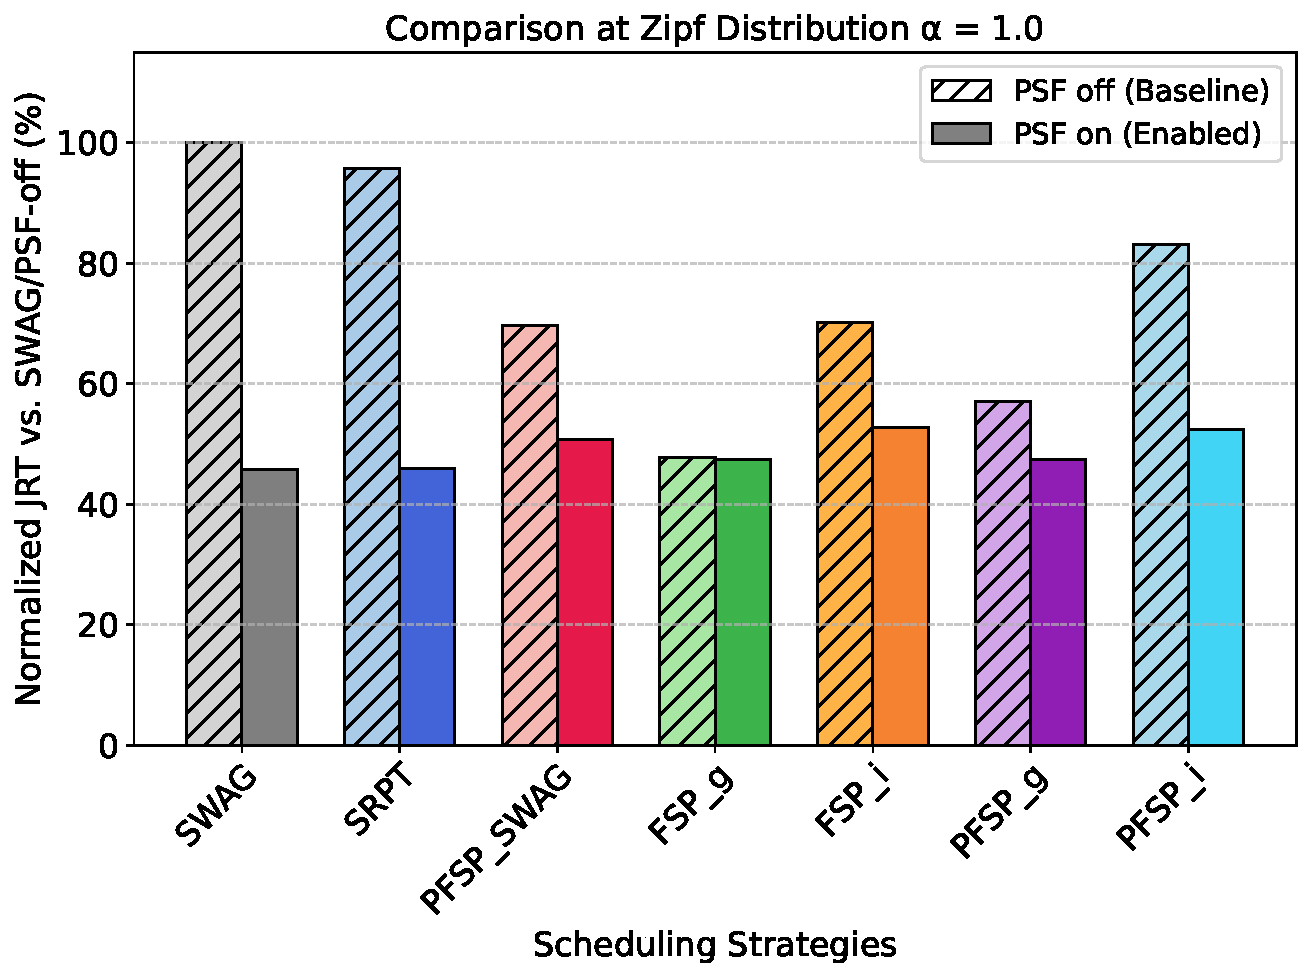
\includegraphics[width=\textwidth]{Image3/PSF_Bar_Ali2017_70_alpha=1.0_dev=0.3.pdf}
        \caption{$\alpha = 1.0$}
    \end{subfigure}
    \hfill
    \begin{subfigure}[b]{0.4\textwidth}
        \centering
        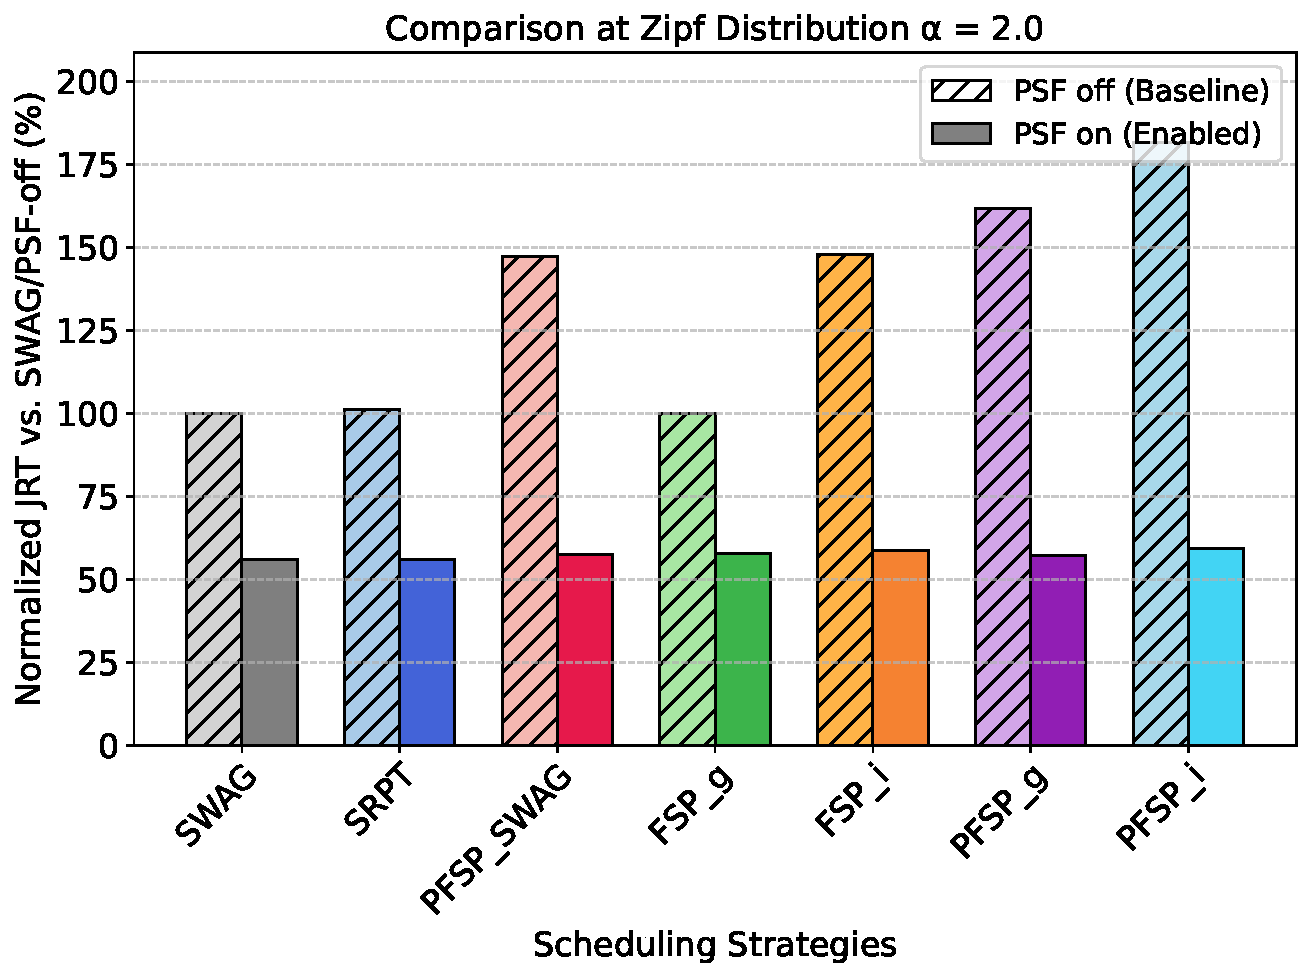
\includegraphics[width=\textwidth]{Image3/PSF_Bar_Ali2017_70_alpha=2.0_dev=0.3.pdf}
        \caption{$\alpha = 2.0$}
    \end{subfigure}

    \caption{Average job response time with/without PSF, 30\% deviation, 70\% utilization, Alibaba 2017}
    \label{fig:JRT_Ali2017_err=0.3}
\end{figure*}

\begin{figure*}[t]
    \centering
    \begin{subfigure}[b]{0.4\textwidth}
        \centering
        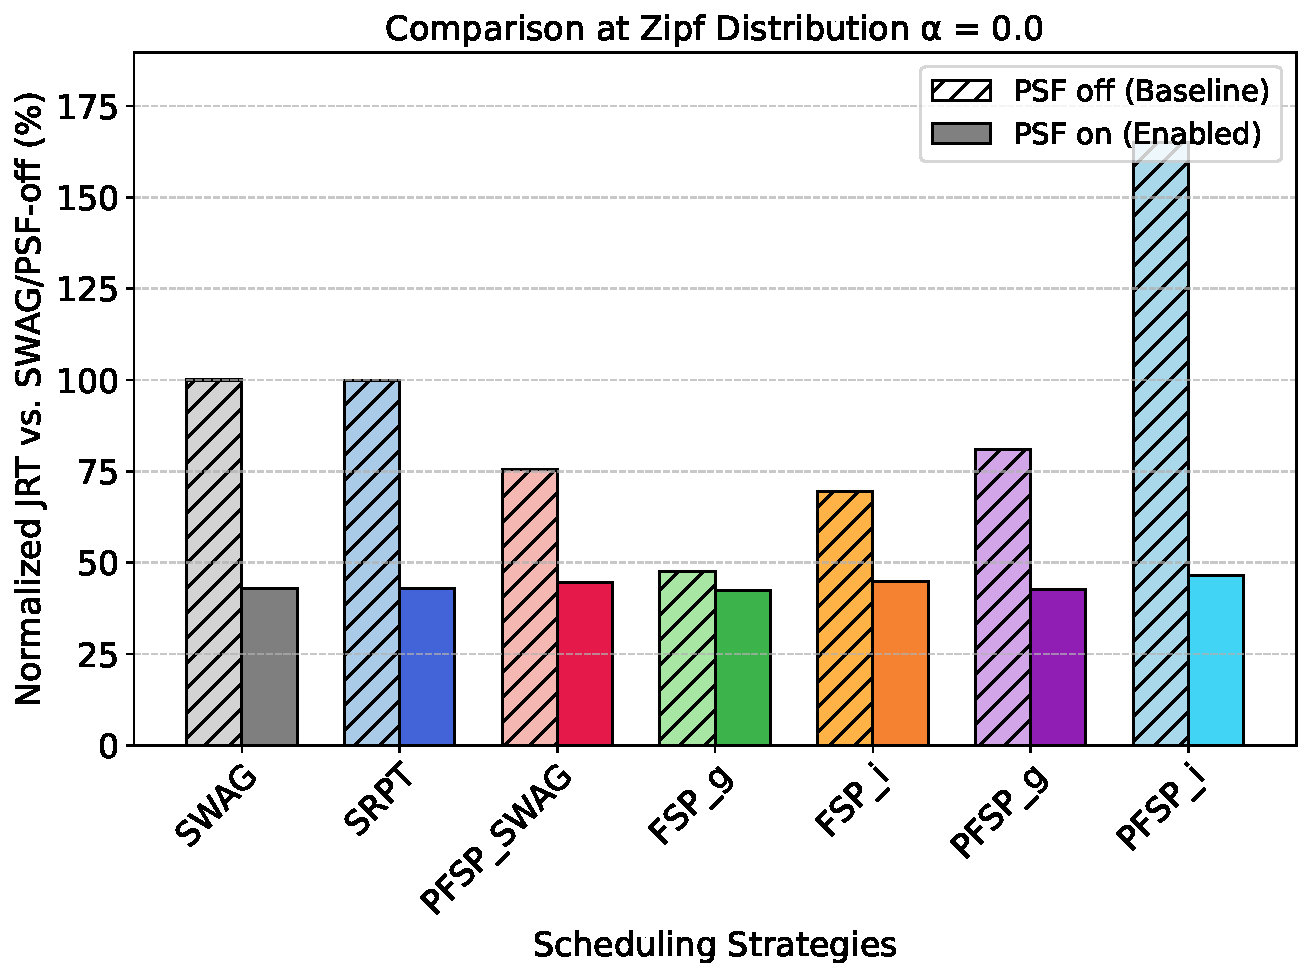
\includegraphics[width=\textwidth]{Image3/PSF_Bar_Ali2017_70_alpha=0.0_dev=0.4.pdf}
        \caption{$\alpha = 0.0$}
    \end{subfigure}
    \hfill
    \begin{subfigure}[b]{0.4\textwidth}
        \centering
        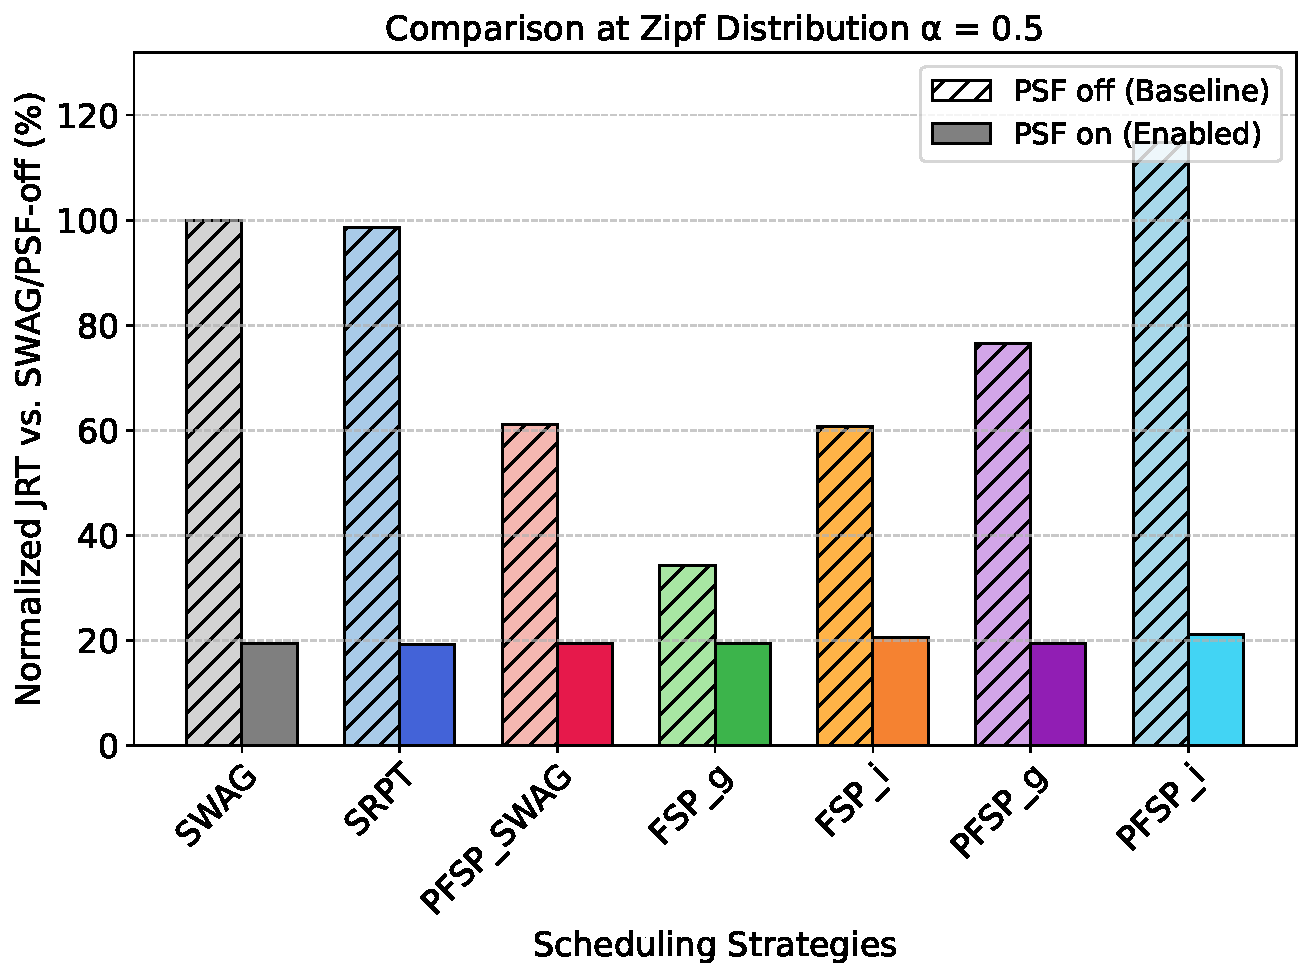
\includegraphics[width=\textwidth]{Image3/PSF_Bar_Ali2017_70_alpha=0.5_dev=0.4.pdf}
        \caption{$\alpha = 0.5$}
    \end{subfigure}
    \vspace{0.8em}
    \begin{subfigure}[b]{0.4\textwidth}
        \centering
        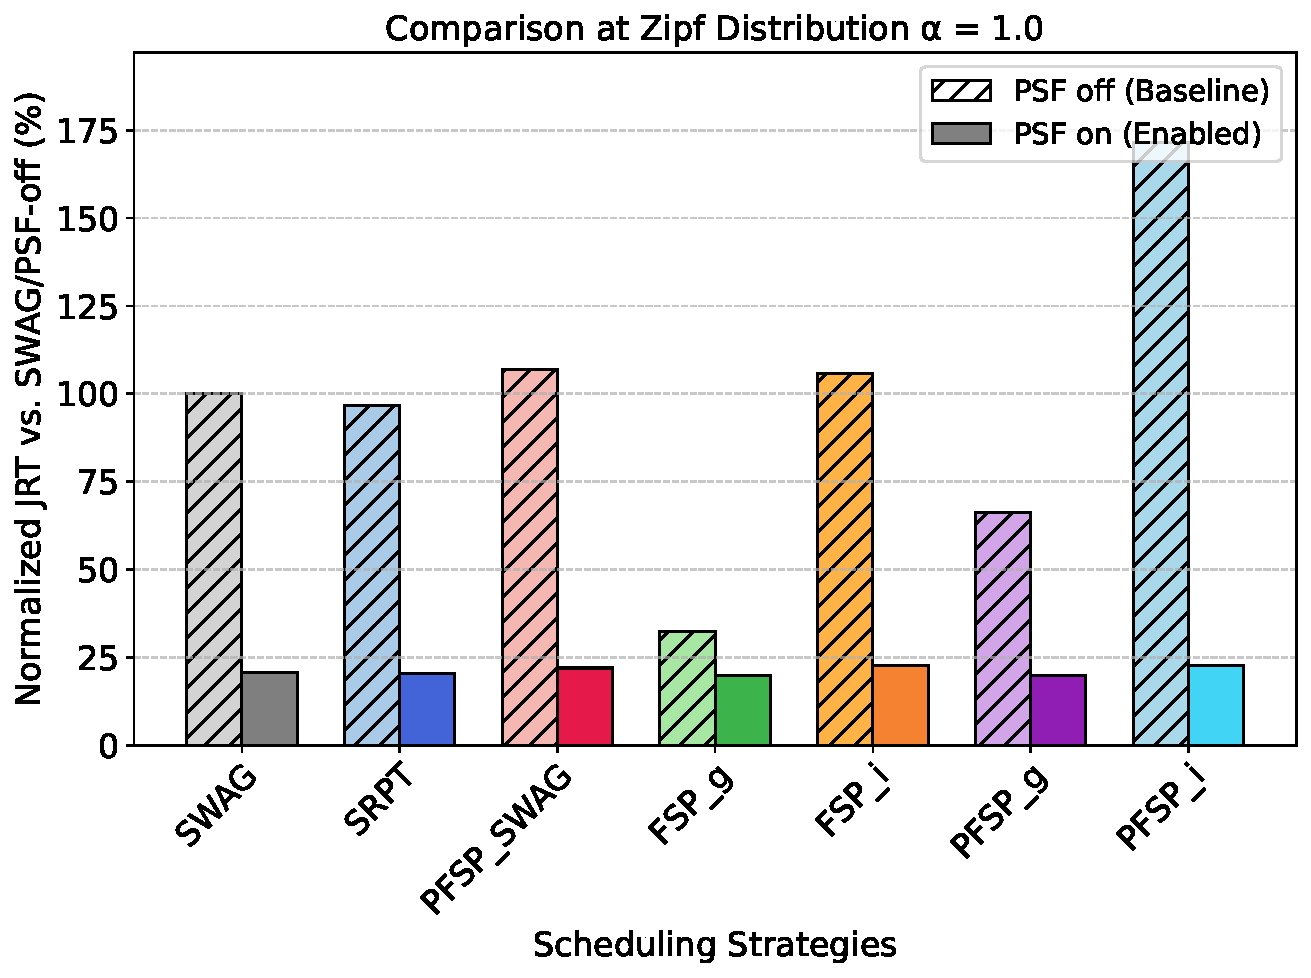
\includegraphics[width=\textwidth]{Image3/PSF_Bar_Ali2017_70_alpha=1.0_dev=0.4.pdf}
        \caption{$\alpha = 1.0$}
    \end{subfigure}
    \hfill
    \begin{subfigure}[b]{0.4\textwidth}
        \centering
        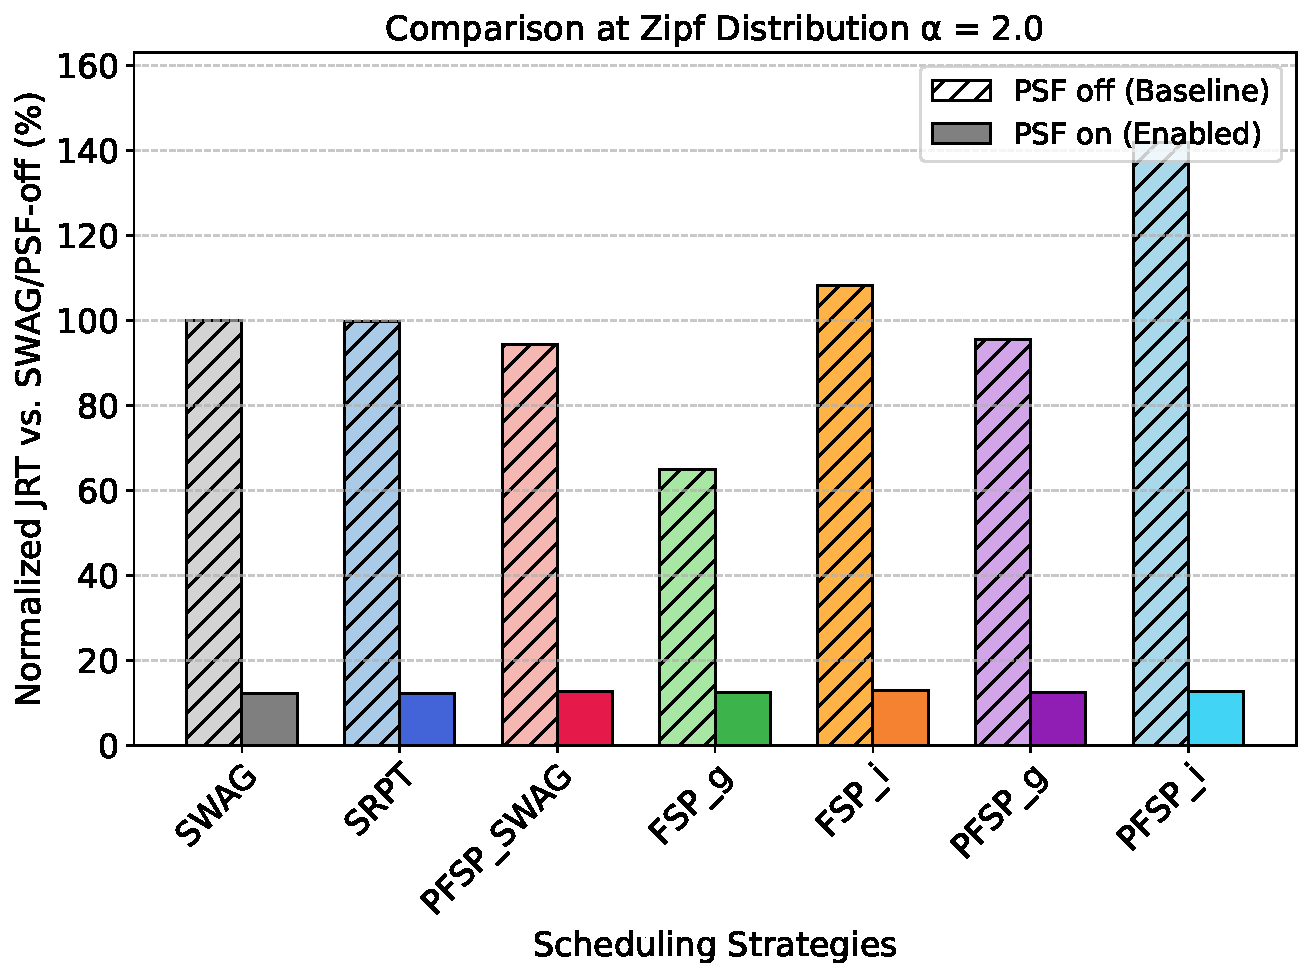
\includegraphics[width=\textwidth]{Image3/PSF_Bar_Ali2017_70_alpha=2.0_dev=0.4.pdf}
        \caption{$\alpha = 2.0$}
    \end{subfigure}

    \caption{Average job response time with/without PSF, 40\% deviation, 70\% utilization, Alibaba 2017}
    \label{fig:JRT_Ali2017_err=0.4}
\end{figure*}

\begin{figure*}[t]
    \centering
    \begin{subfigure}[b]{0.4\textwidth}
        \centering
        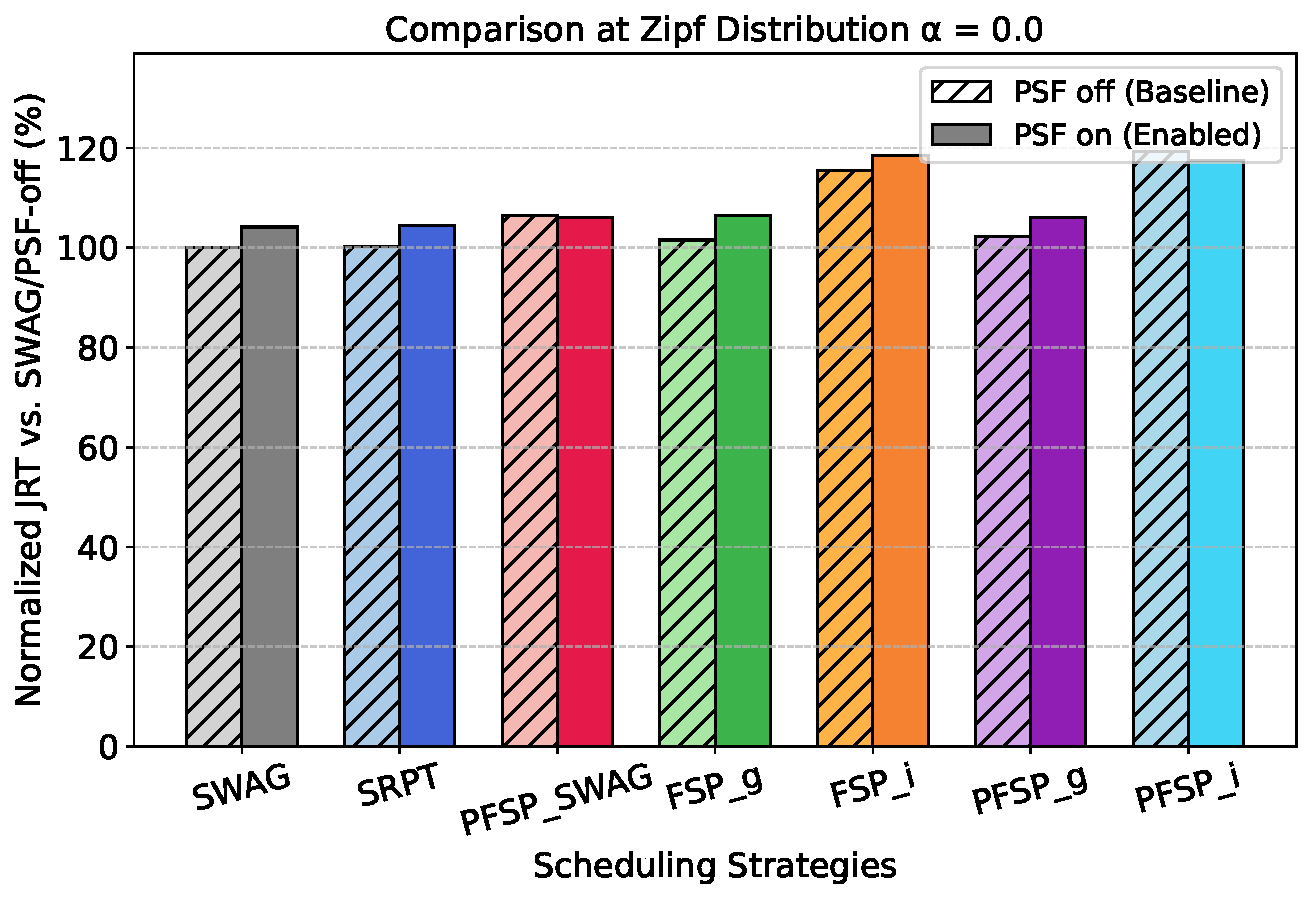
\includegraphics[width=\textwidth]{Image3/PSF_Bar_Ali2018_4_70_alpha=0.0_dev=0.1.pdf}
        \caption{$\alpha = 0.0$}
    \end{subfigure}
    \hfill
    \begin{subfigure}[b]{0.4\textwidth}
        \centering
        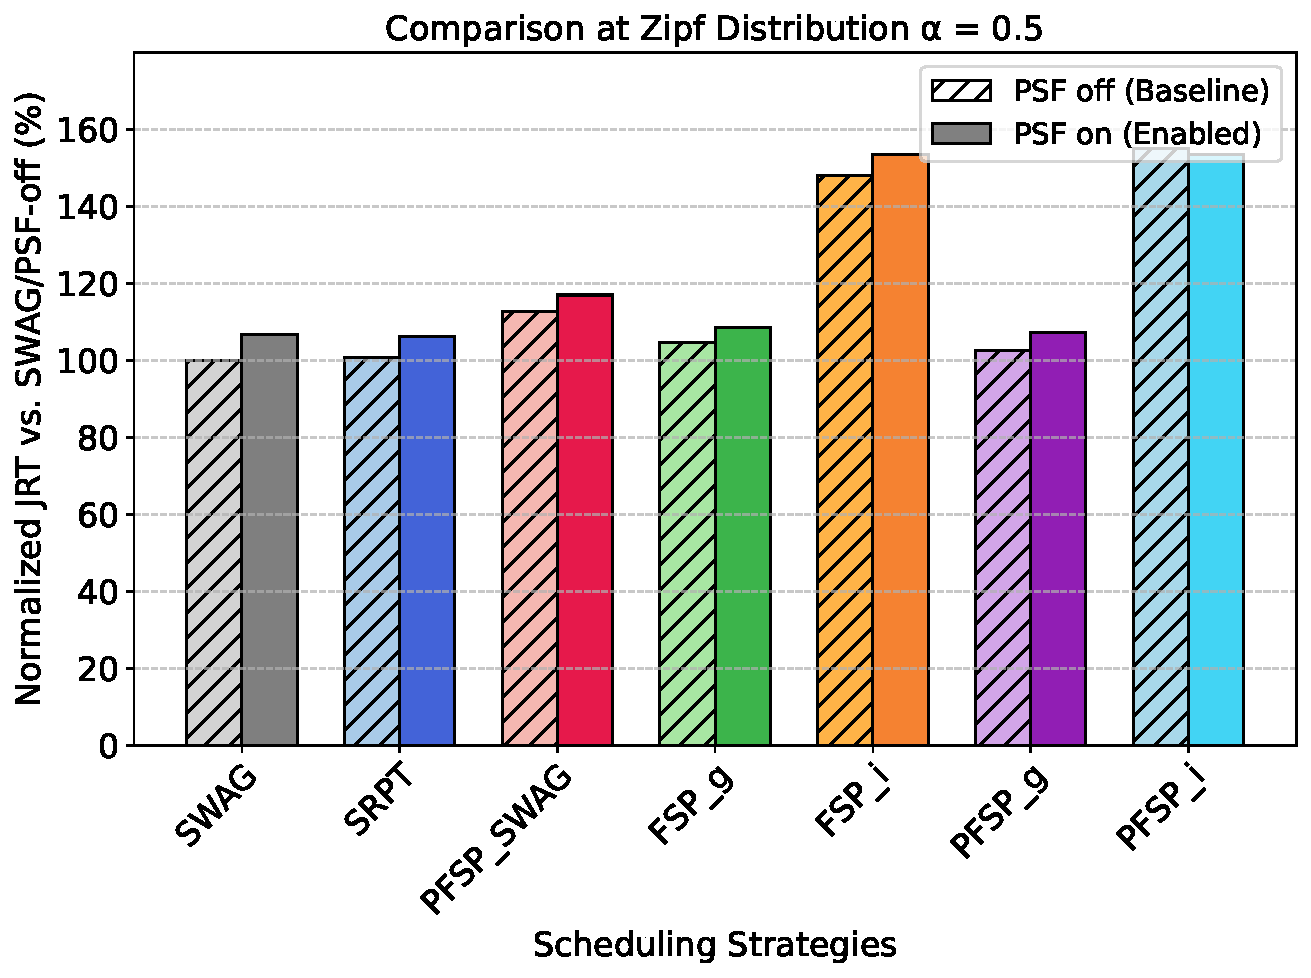
\includegraphics[width=\textwidth]{Image3/PSF_Bar_Ali2018_4_70_alpha=0.5_dev=0.1.pdf}
        \caption{$\alpha = 0.5$}
    \end{subfigure}
    \vspace{0.8em}
    \begin{subfigure}[b]{0.4\textwidth}
        \centering
        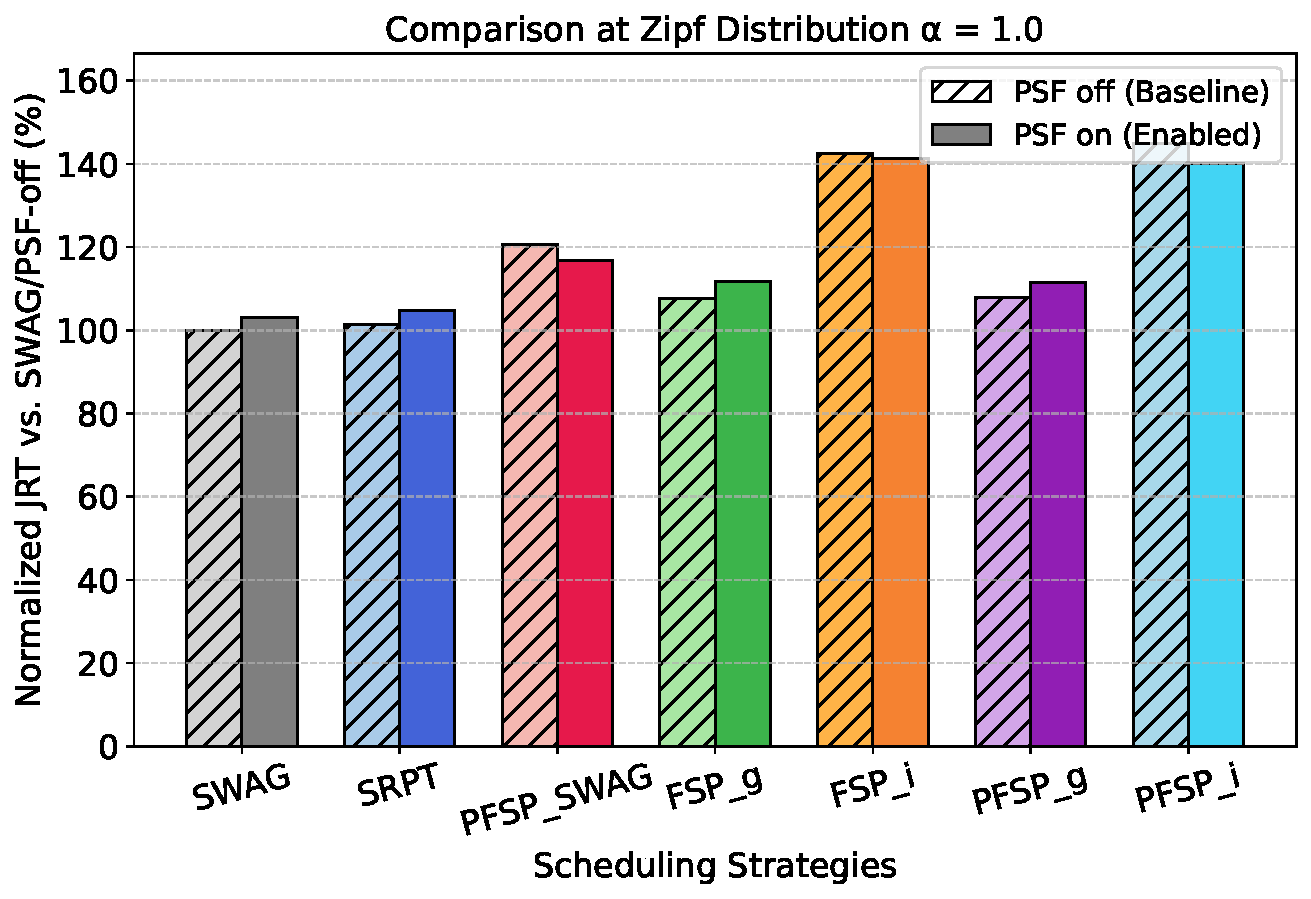
\includegraphics[width=\textwidth]{Image3/PSF_Bar_Ali2018_4_70_alpha=1.0_dev=0.1.pdf}
        \caption{$\alpha = 1.0$}
    \end{subfigure}
    \hfill
    \begin{subfigure}[b]{0.4\textwidth}
        \centering
        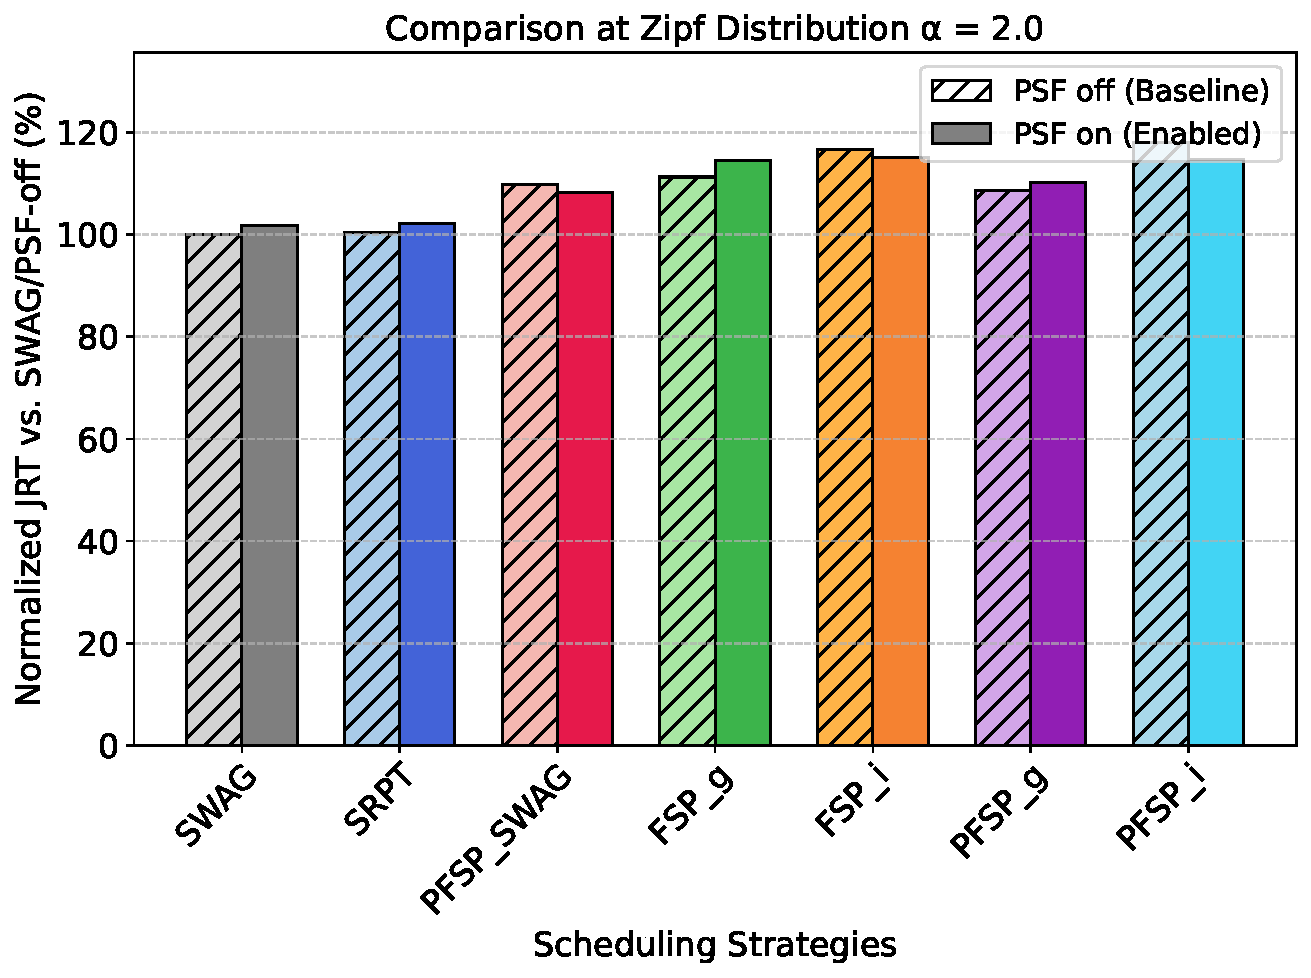
\includegraphics[width=\textwidth]{Image3/PSF_Bar_Ali2018_4_70_alpha=2.0_dev=0.1.pdf}
        \caption{$\alpha = 2.0$}
    \end{subfigure}

    \caption{Average job response time with/without PSF, 10\% deviation, 70\% utilization, Alibaba 2018}
    \label{fig:JRT_Ali2018_err=0.1}
\end{figure*}

\begin{figure*}[t]
    \centering
    \begin{subfigure}[b]{0.4\textwidth}
        \centering
        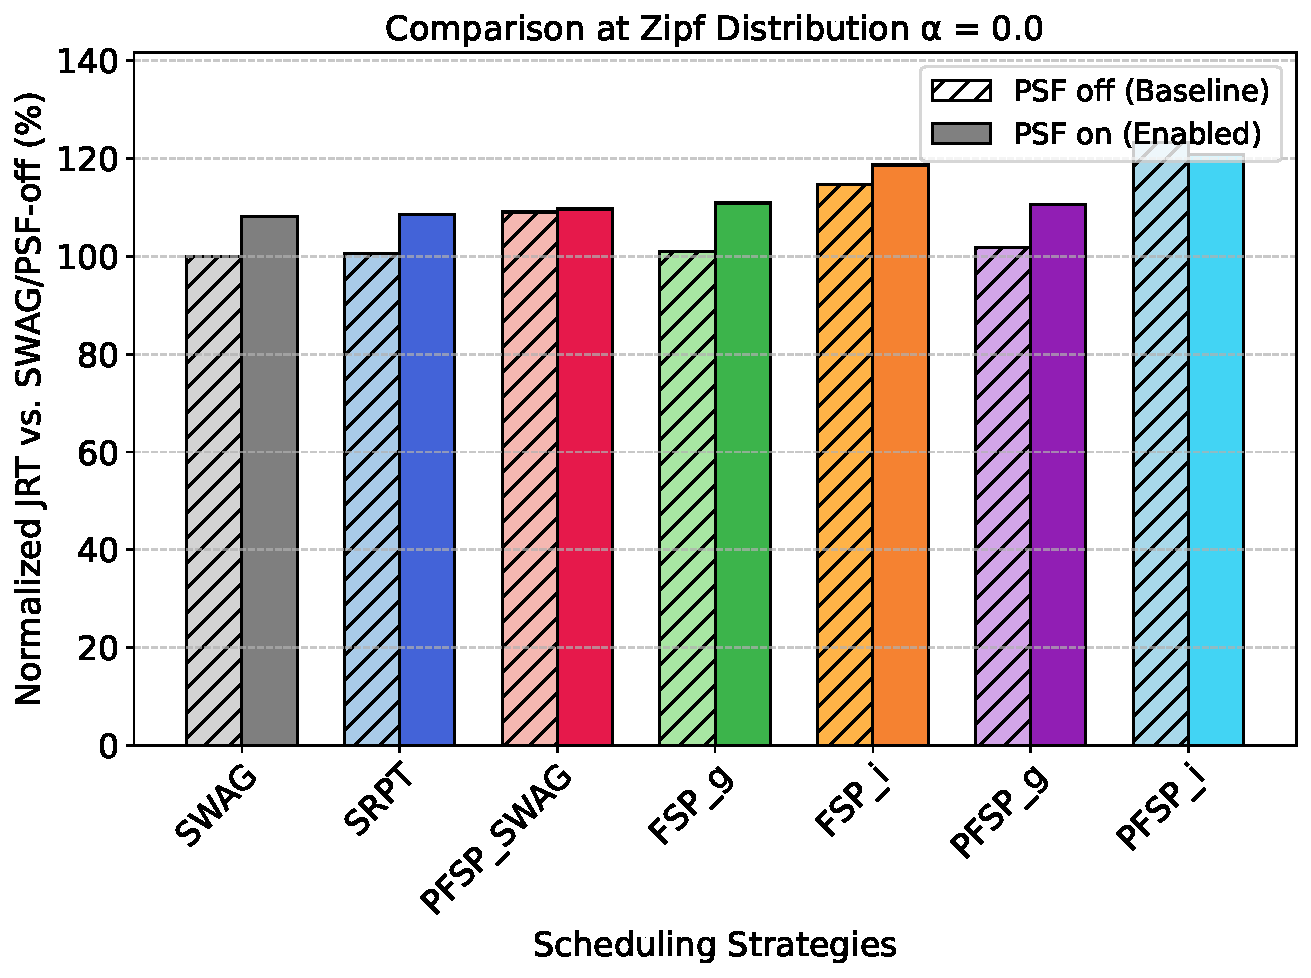
\includegraphics[width=\textwidth]{Image3/PSF_Bar_Ali2018_4_70_alpha=0.0_dev=0.2.pdf}
        \caption{$\alpha = 0.0$}
    \end{subfigure}
    \hfill
    \begin{subfigure}[b]{0.4\textwidth}
        \centering
        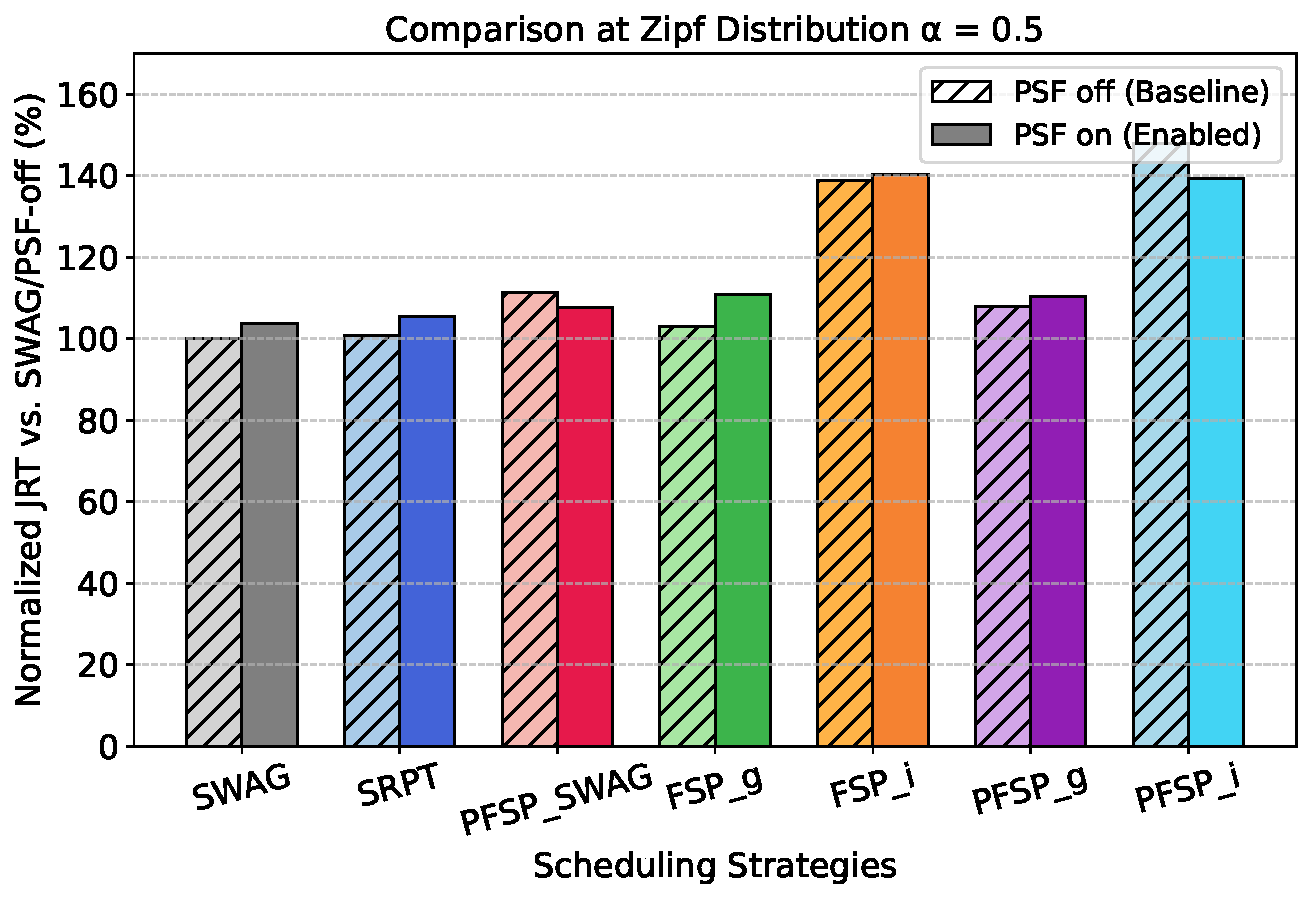
\includegraphics[width=\textwidth]{Image3/PSF_Bar_Ali2018_4_70_alpha=0.5_dev=0.2.pdf}
        \caption{$\alpha = 0.5$}
    \end{subfigure}
    \vspace{0.8em}
    \begin{subfigure}[b]{0.4\textwidth}
        \centering
        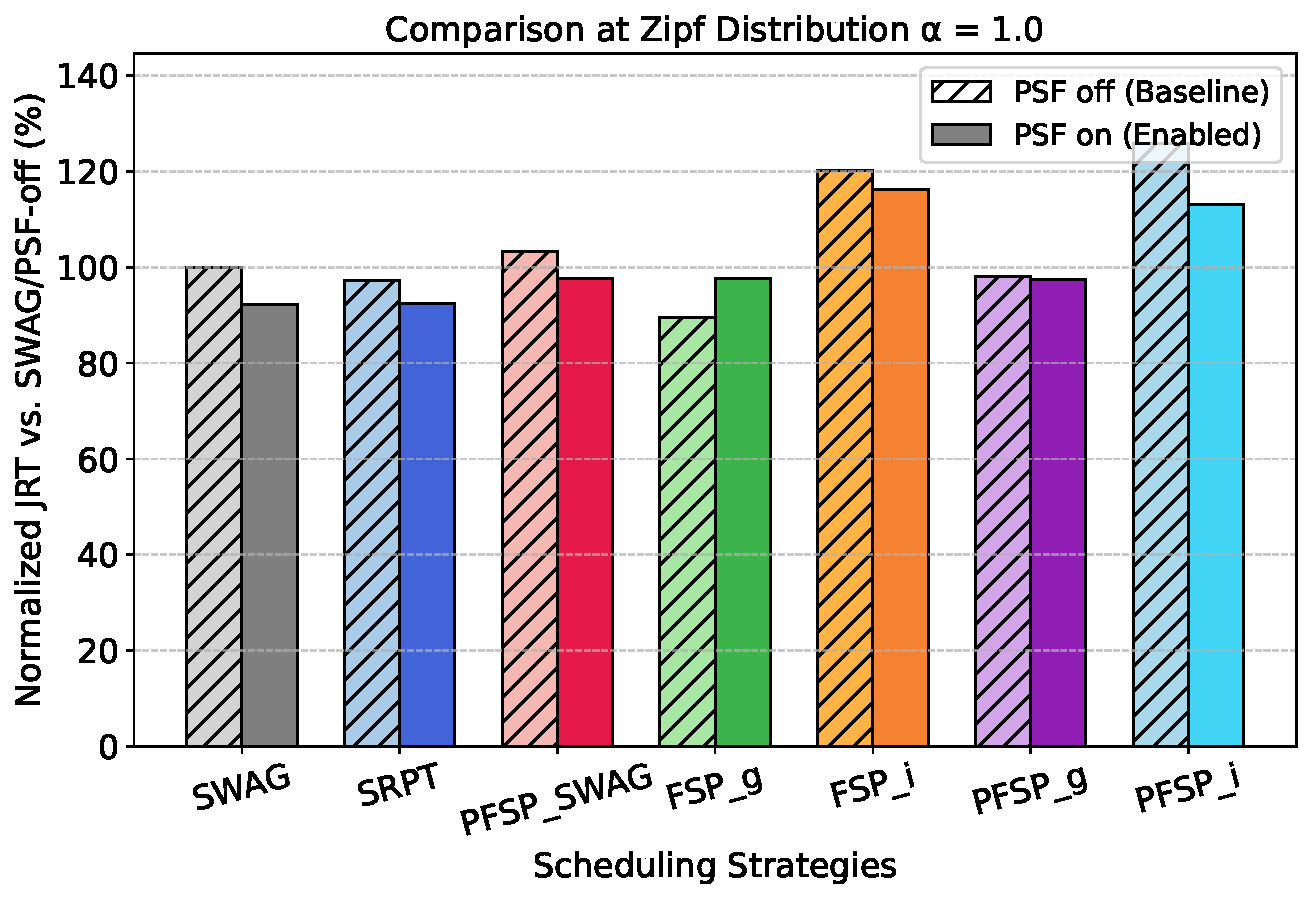
\includegraphics[width=\textwidth]{Image3/PSF_Bar_Ali2018_4_70_alpha=1.0_dev=0.2.pdf}
        \caption{$\alpha = 1.0$}
    \end{subfigure}
    \hfill
    \begin{subfigure}[b]{0.4\textwidth}
        \centering
        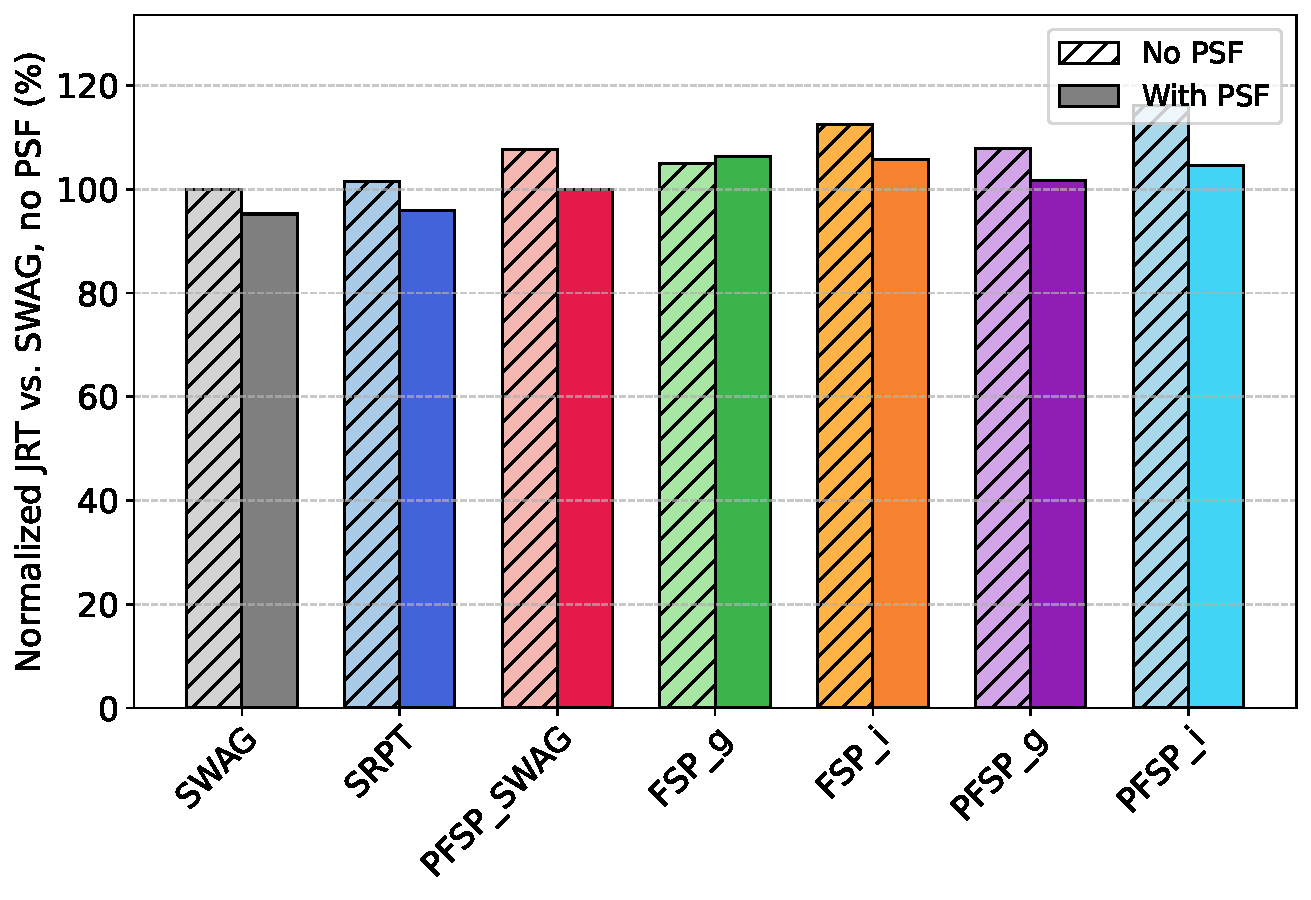
\includegraphics[width=\textwidth]{Image3/PSF_Bar_Ali2018_4_70_alpha=2.0_dev=0.2.pdf}
        \caption{$\alpha = 2.0$}
    \end{subfigure}

    \caption{Average job response time with/without PSF, 20\% deviation, 70\% utilization, Alibaba 2018}
    \label{fig:JRT_Ali2018_err=0.2}
\end{figure*}

\begin{figure*}[t]
    \centering
    \begin{subfigure}[b]{0.4\textwidth}
        \centering
        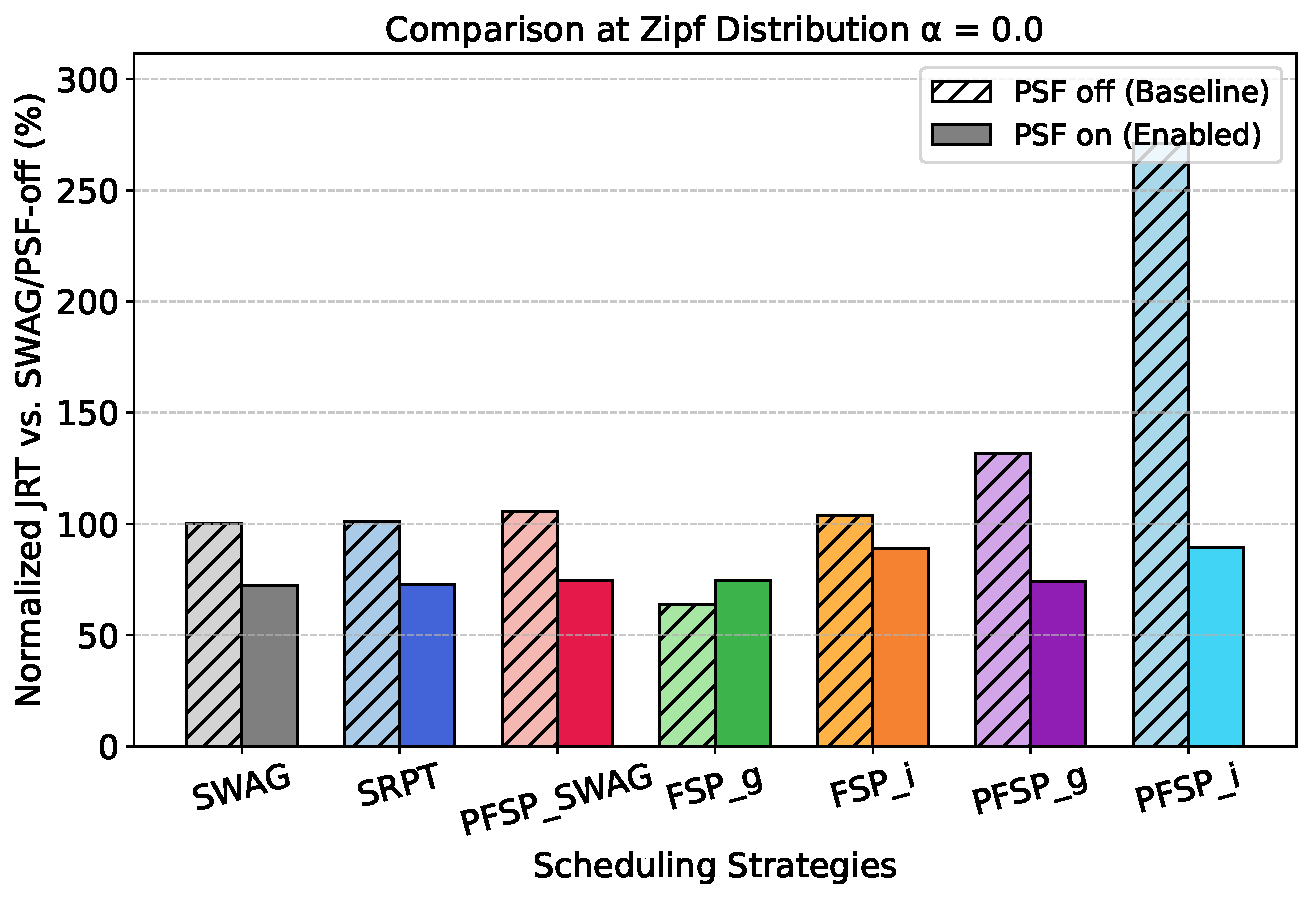
\includegraphics[width=\textwidth]{Image3/PSF_Bar_Ali2018_4_70_alpha=0.0_dev=0.3.pdf}
        \caption{$\alpha = 0.0$}
    \end{subfigure}
    \hfill
    \begin{subfigure}[b]{0.4\textwidth}
        \centering
        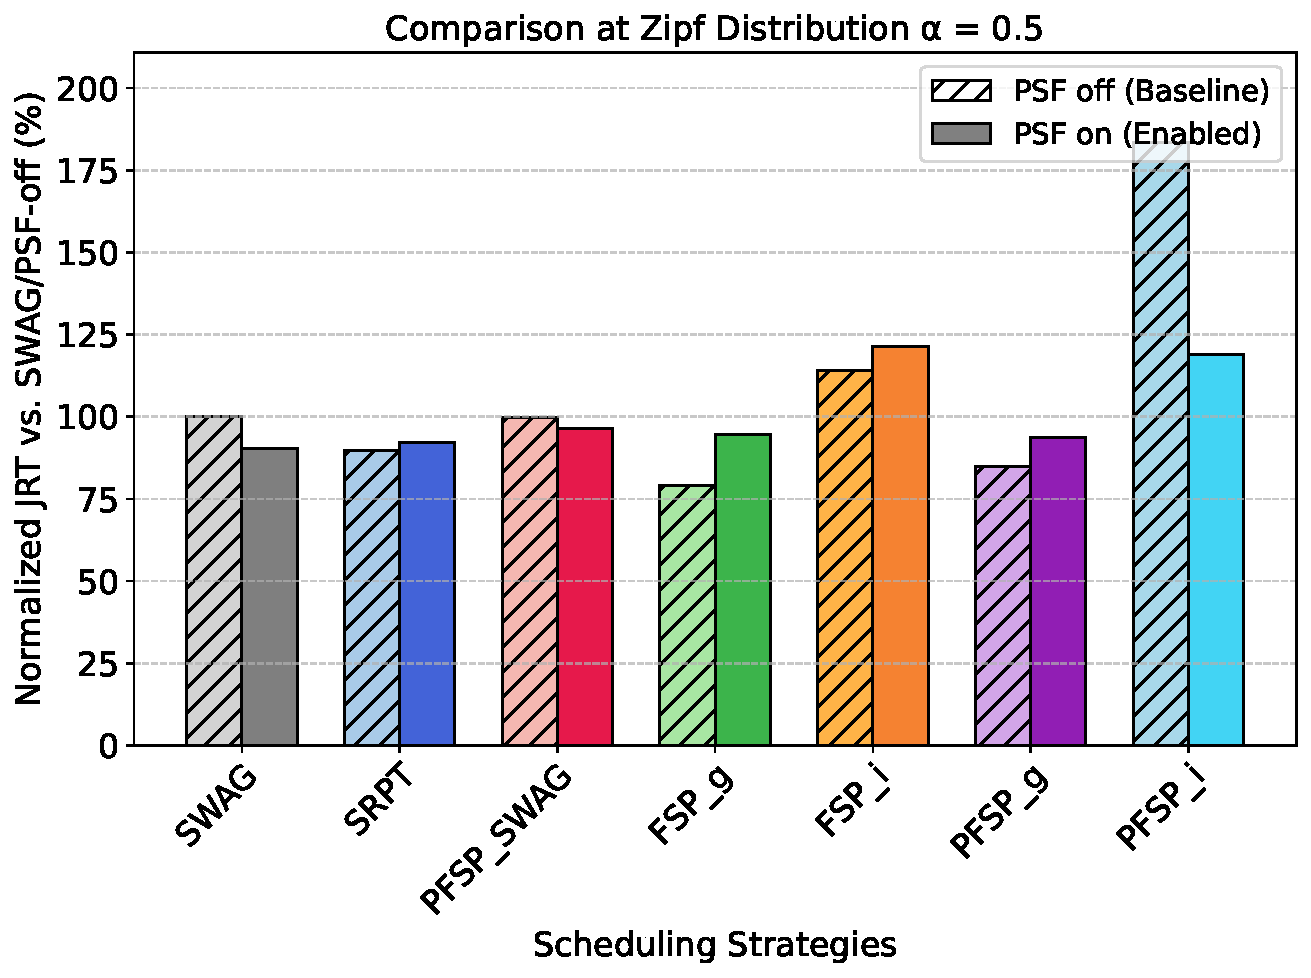
\includegraphics[width=\textwidth]{Image3/PSF_Bar_Ali2018_4_70_alpha=0.5_dev=0.3.pdf}
        \caption{$\alpha = 0.5$}
    \end{subfigure}
    \vspace{0.8em}
    \begin{subfigure}[b]{0.4\textwidth}
        \centering
        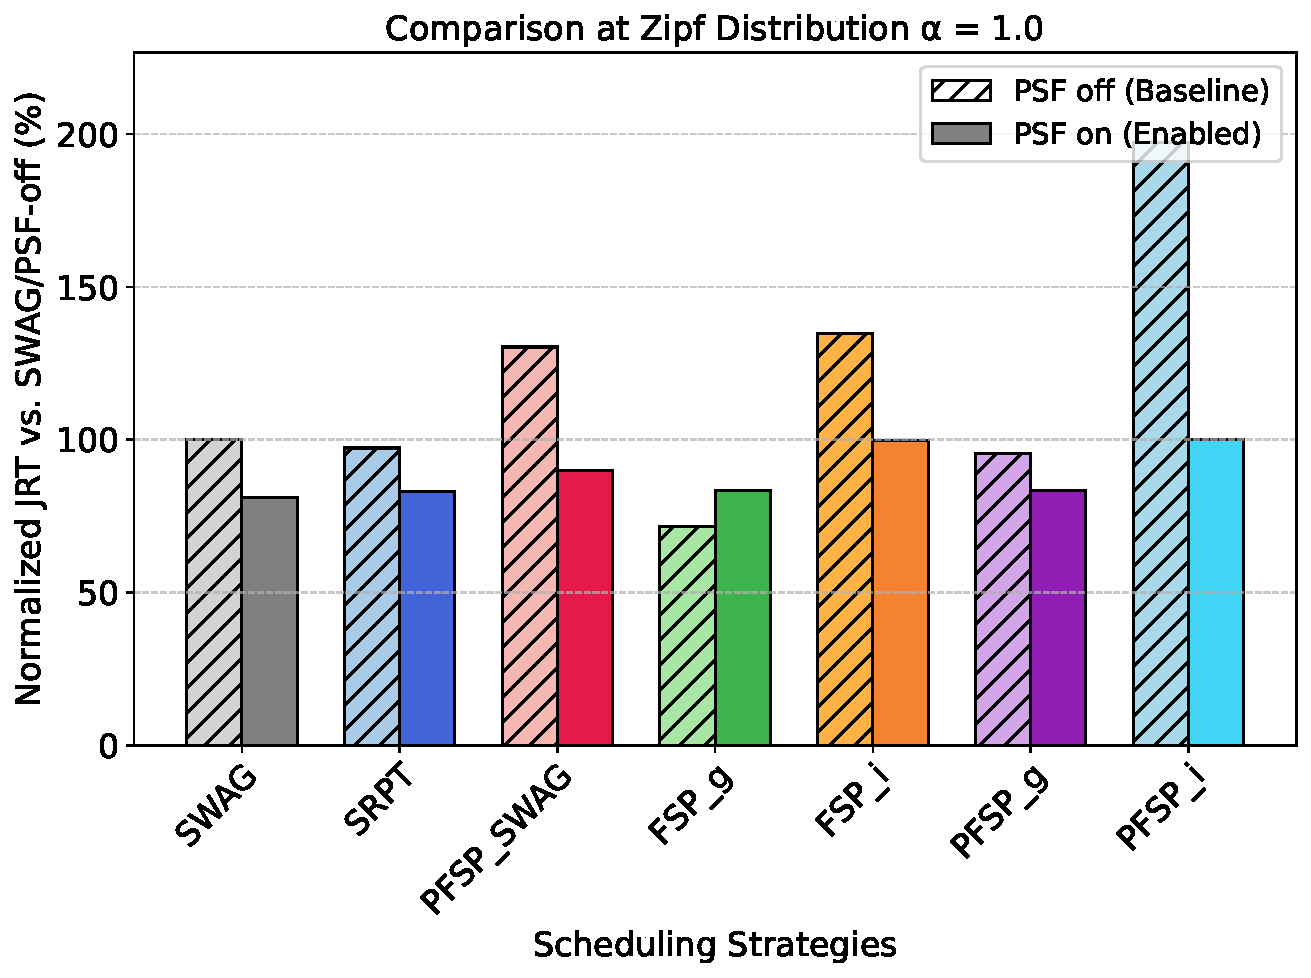
\includegraphics[width=\textwidth]{Image3/PSF_Bar_Ali2018_4_70_alpha=1.0_dev=0.3.pdf}
        \caption{$\alpha = 1.0$}
    \end{subfigure}
    \hfill
    \begin{subfigure}[b]{0.4\textwidth}
        \centering
        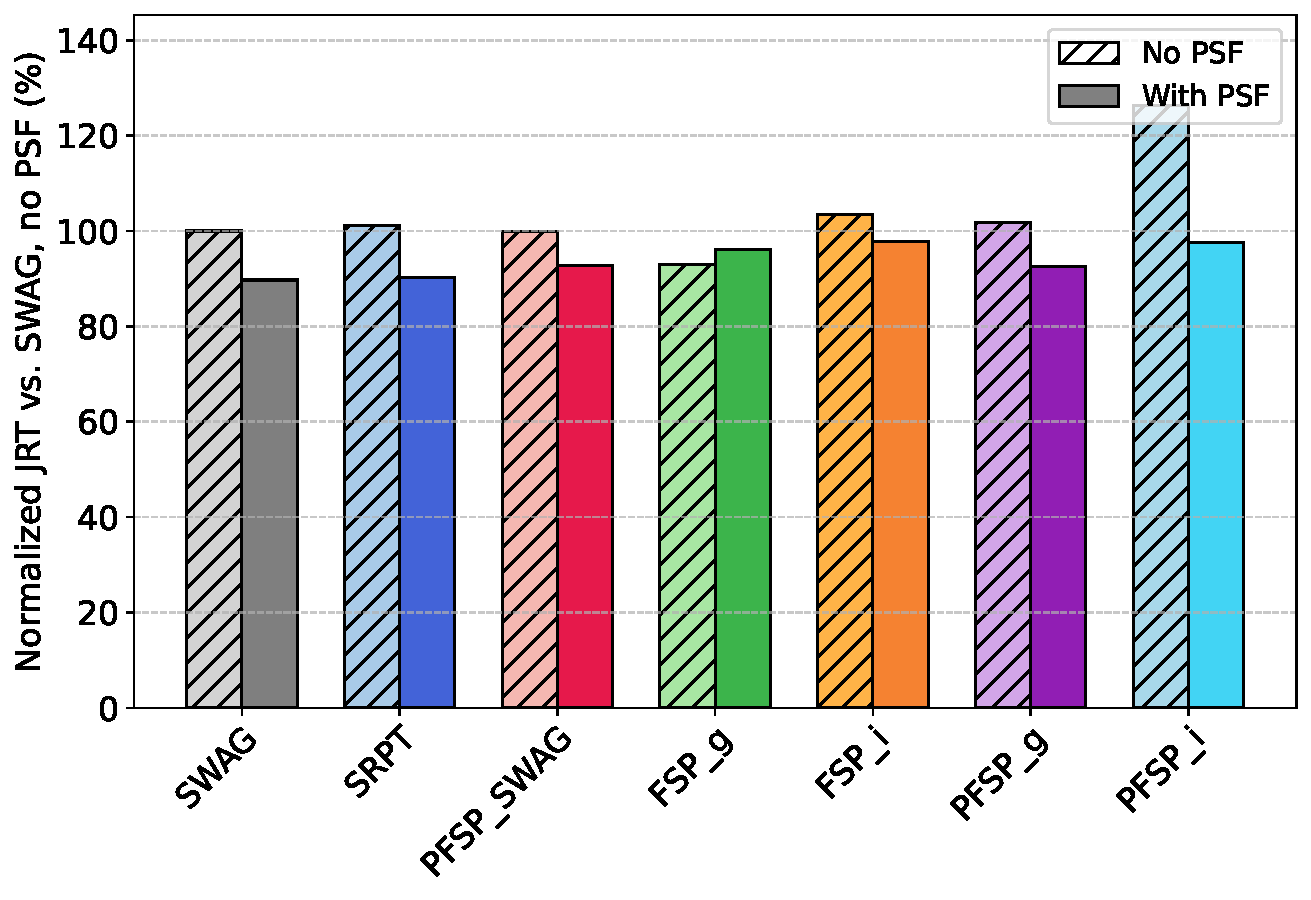
\includegraphics[width=\textwidth]{Image3/PSF_Bar_Ali2018_4_70_alpha=2.0_dev=0.3.pdf}
        \caption{$\alpha = 2.0$}
    \end{subfigure}

    \caption{Average job response time with/without PSF, 30\% deviation, 70\% utilization, Alibaba 2018}
    \label{fig:JRT_Ali2018_err=0.3}
\end{figure*}

\begin{figure*}[t]
    \centering
    \begin{subfigure}[b]{0.4\textwidth}
        \centering
        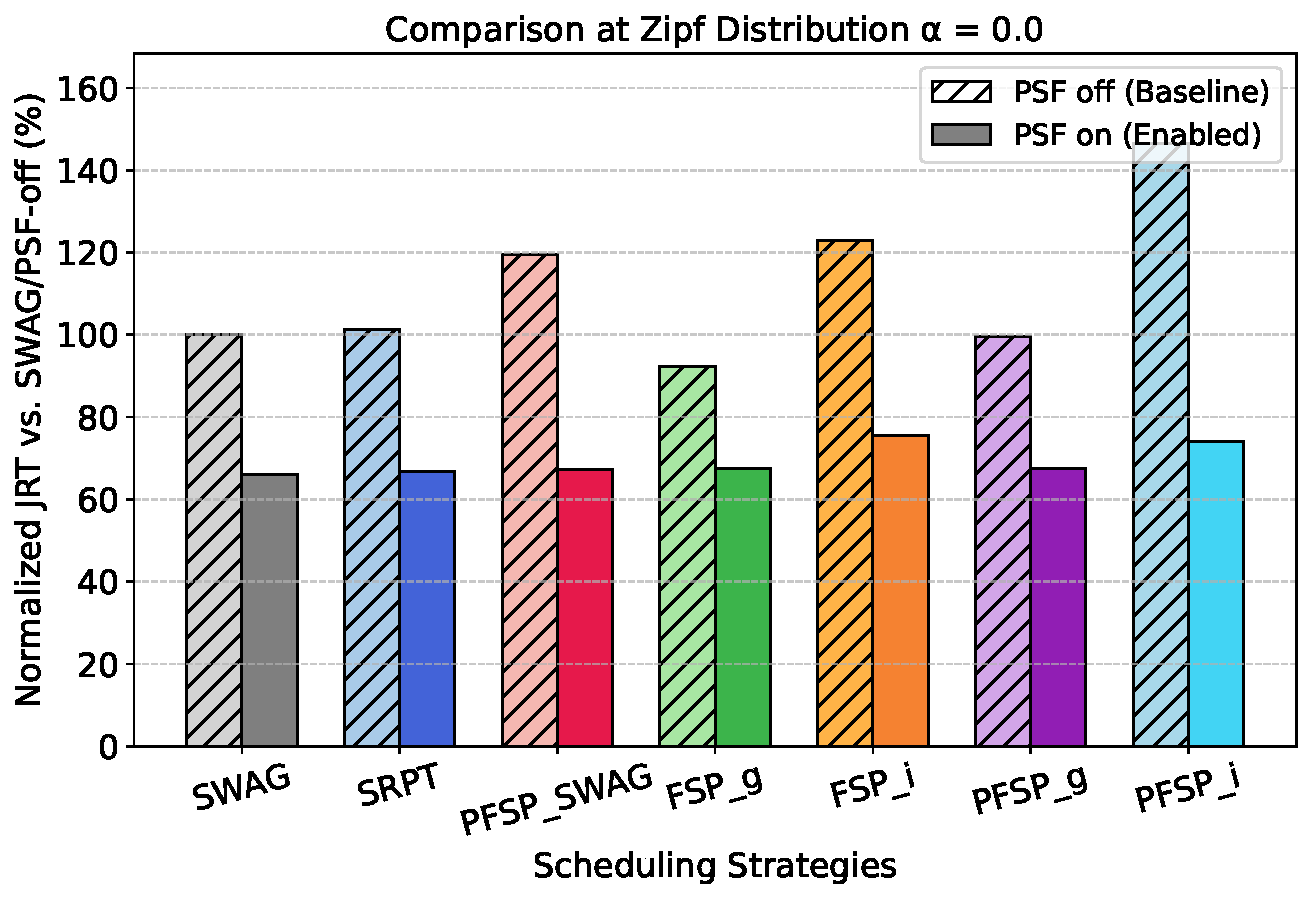
\includegraphics[width=\textwidth]{Image3/PSF_Bar_Ali2018_4_70_alpha=0.0_dev=0.4.pdf}
        \caption{$\alpha = 0.0$}
    \end{subfigure}
    \hfill
    \begin{subfigure}[b]{0.4\textwidth}
        \centering
        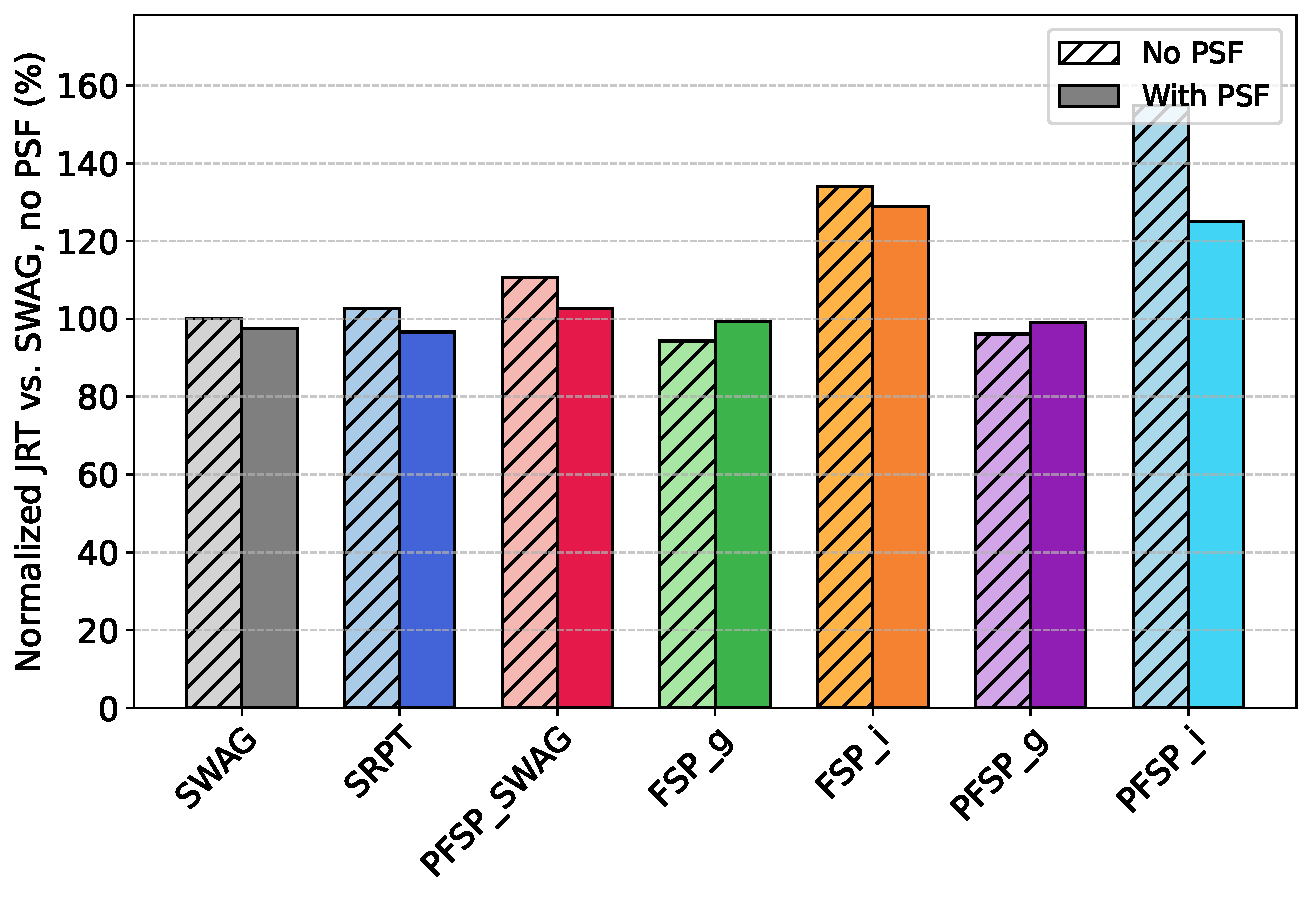
\includegraphics[width=\textwidth]{Image3/PSF_Bar_Ali2018_4_70_alpha=0.5_dev=0.4.pdf}
        \caption{$\alpha = 0.5$}
    \end{subfigure}
    \vspace{0.8em}
    \begin{subfigure}[b]{0.4\textwidth}
        \centering
        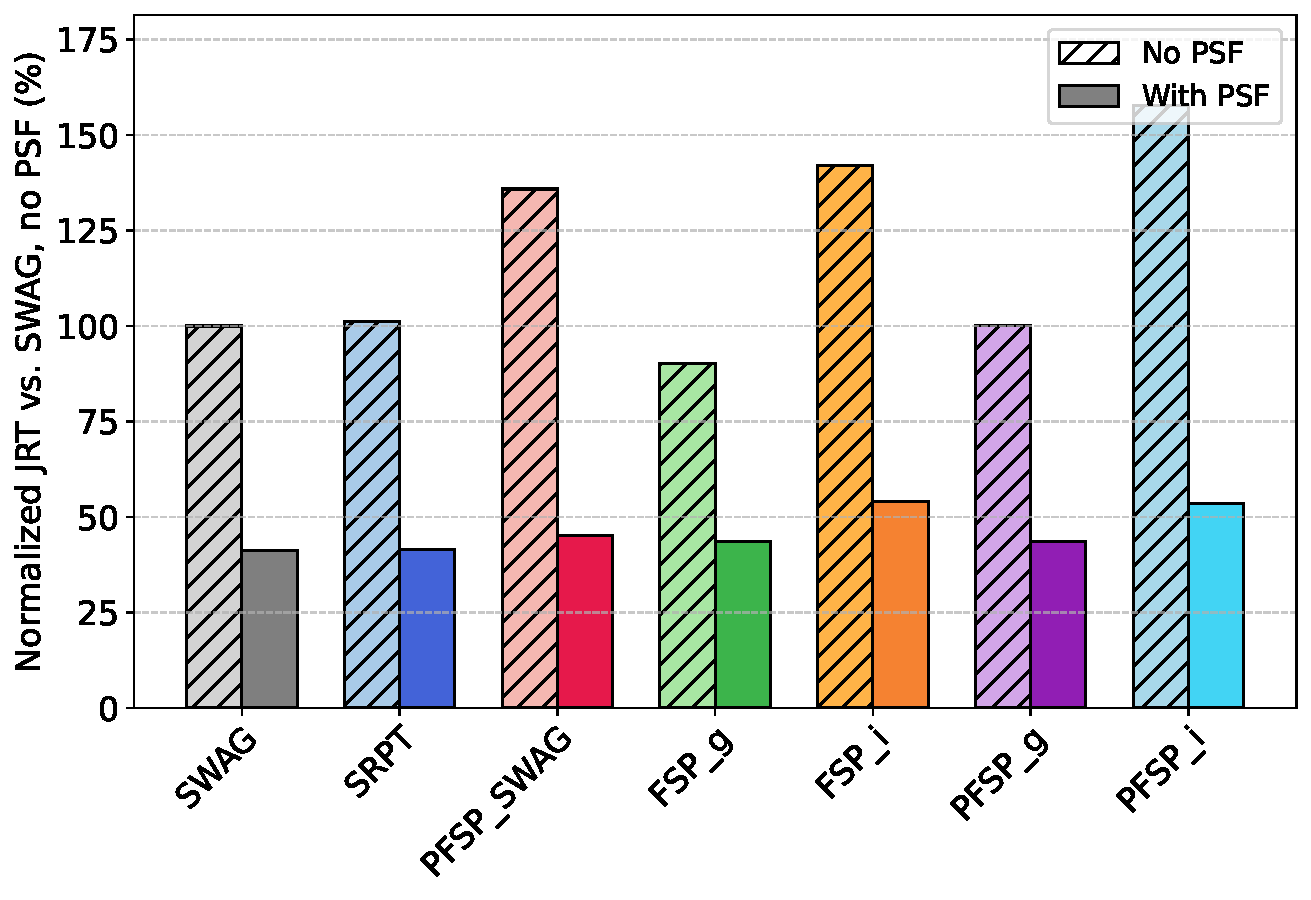
\includegraphics[width=\textwidth]{Image3/PSF_Bar_Ali2018_4_70_alpha=1.0_dev=0.4.pdf}
        \caption{$\alpha = 1.0$}
    \end{subfigure}
    \hfill
    \begin{subfigure}[b]{0.4\textwidth}
        \centering
        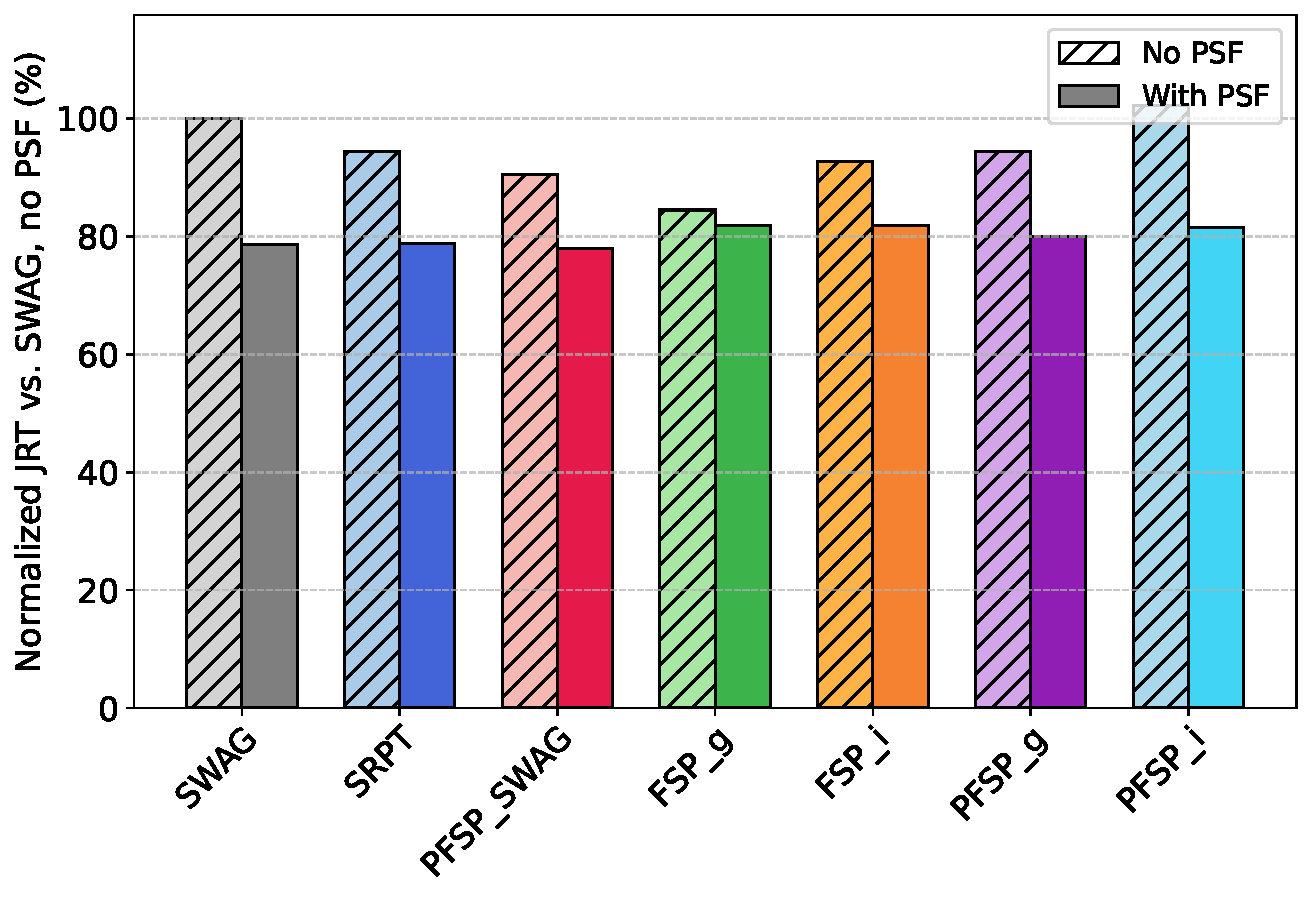
\includegraphics[width=\textwidth]{Image3/PSF_Bar_Ali2018_4_70_alpha=2.0_dev=0.4.pdf}
        \caption{$\alpha = 2.0$}
    \end{subfigure}

    \caption{Average job response time with/without PSF, 40\% deviation, 70\% utilization, Alibaba 2018}
    \label{fig:JRT_Ali2018_err=0.4}
\end{figure*}

Figures \ref{fig:JRT_Ali2017_err=0.1} through \ref{fig:JRT_Ali2018_err=0.4} illustrate the average job response time  under different deviations of job load estimations for both datasets. To facilitate comparison, the response time of the baseline SWAG policy—without the PSF mechanism—is normalized to $100\%$, with all other policies expressed relative to this baseline. Overall, the performance difference between policies with and without the PSF mechanism remains minor across most scenarios. However, in certain cases (e.g., Figure \ref{fig:JRT_Ali2017_err=0.4}), integrating the PSF mechanism yields a substantial reduction in average job response time across all evaluated scheduling policies. In conclusion, incorporating the PSF mechanism into the evaluated scheduling policies significantly mitigates PS deadline violations while maintaining comparable or superior average job response times. 


\section{Summary}
\label{sec:conclusion3}

In this chapter, we investigated how to achieve the dual objective between efficiency and long-term fairness in distributed job execution by extending the theory of protective scheduling in the single-site case. We established the distributed slack system to help judge the system protectiveness using two perspectives: the Global Slack ($GS$) scheme and the Independent Slack ($IS$) scheme. Through theoretical analysis, we proved that dynamic job arrivals inherently prevent global order-based policies from guaranteeing strict protectiveness under the $GS$ scheme. To overcome this dilemma, we proposed PFSP\_x, a novel heuristic scheduling framework that adopts the $IS$ scheme to ensure protectiveness while approximating a hint job order derived by any efficiency-targeted policies. We also developed a series of extension policies based on the single-site policies FSP, PFSP and OFSP as the baselines. Extensive trace-driven simulations using Alibaba cluster datasets demonstrated that our proposed PFSP\_SWAG policy achieves the highest job processing efficiency among all strictly protective policies evaluated. Furthermore, the extension policy PFSP\_g under the $GS$ scheme is shown capable of delivering average job response times comparable to efficiency-targeted policies with negligible fairness violations. Ultimately, these complementary strategies equip distributed systems to flexibly navigate the delicate trade-off between job processing efficiency and long-term fairness.
%In conclusion, we present two primary scheduling policies, by which the distributed system is empowered to flexibly adapt to different system requirements, effectively balancing the delicate trade-off between job processing efficiency and long-term job fairness.



%----------------------------------------------------------------------------------------
%	THESIS CONTENT - APPENDICES
%----------------------------------------------------------------------------------------

\addtocontents{toc}{\vspace{0.8em}} % Add a gap in the Contents, for aesthetics

% \appendix % Cue to tell LaTeX that the following 'chapters' are Appendices

% Include the appendices of the thesis as separate files from the Appendices folder
% Uncomment the lines as you write the Appendices

%!TEX root=../mythesis.tex
% Appendix A

\chapter{Number of violations to PS deadline with/without PSF} % Main appendix title

\label{AppendixA} % For referencing this appendix elsewhere, use \ref{AppendixA}

\begin{table}[t]
\centering
\caption{Number of violations to PS deadline with/without PSF, 10\% deviation, 70\% utilization, Alibaba 2018}
\label{tab:PSF_comparison1}
\resizebox{\textwidth}{!}{\begin{tabular}{l cccc c cccc}
\toprule
& \multicolumn{4}{c}{\textbf{Without PSF}} & & \multicolumn{4}{c}{\textbf{With PSF}} \\
\cmidrule{2-5} \cmidrule{7-10}
\textbf{Policy} & $\alpha=0.0$ & $\alpha=0.5$ & $\alpha=1.0$ & $\alpha=2.0$ & & $\alpha=0.0$ & $\alpha=0.5$ & $\alpha=1.0$ & $\alpha=2.0$ \\
\midrule
SWAG & 92  & 98 & 188 & 178 & & 44 & 47 & 62 & 76 \\
SRPT & 108 & 91 & 200 & 183 & & 55 & 52 & 69 & 81 \\
PFSP\_g & 81 & 40 & 133 & 149 & & 30 & 19 & 27 & 62 \\
FSP\_g & 53 & 27 & 37 & 30 & & 29 & 20 & 25 & 65 \\
PFSP\_SWAG & 394 & 247 & 461 & 276 & & 39 & 41 & 31 & 37 \\
PFSP\_i & 423 & 350 & 513 & 307 & &  41 & 37 & 37 & 42 \\
FSP\_i & 196 & 102 & 258 & 137 & & 36 & 34 & 31 & 36 \\
\bottomrule
\end{tabular}}
\end{table}

\begin{table}[t]
\centering
\caption{Number of violations to PS deadline with/without PSF, 20\% deviation, 70\% utilization, Alibaba 2018}
\label{tab:PSF_comparison2}
\resizebox{\textwidth}{!}{
\begin{tabular}{l cccc c cccc}
\toprule
& \multicolumn{4}{c}{\textbf{Without PSF}} & & \multicolumn{4}{c}{\textbf{With PSF}} \\
\cmidrule{2-5} \cmidrule{7-10}
\textbf{Policy} & $\alpha=0.0$ & $\alpha=0.5$ & $\alpha=1.0$ & $\alpha=2.0$ & & $\alpha=0.0$ & $\alpha=0.5$ & $\alpha=1.0$ & $\alpha=2.0$ \\
\midrule
SWAG & 145  & 209 & 425 & 398 & & 38 & 63 & 65 & 90 \\
SRPT & 163 & 209 & 394 & 408 & & 48 & 64 & 67 & 84 \\
PFSP\_g & 144 & 216 & 315 & 346 & & 34 & 33 & 45 & 70 \\
FSP\_g & 70 & 52 & 99 & 94 & & 33 & 32 & 44 & 73 \\
PFSP\_SWAG & 450 & 564 & 745 & 541 & & 45 & 55 & 53 & 51 \\
PFSP\_i & 498 & 625 & 774 & 536 & &  46 & 58 & 51 & 49 \\
FSP\_i & 185 & 293 & 355 & 281 & & 44 & 53 & 50 & 48 \\
\bottomrule
\end{tabular}}
\end{table}

\begin{table}[t]
\centering
\caption{Number of violations to PS deadline with/without PSF, 30\% deviation, 70\% utilization, Alibaba 2018}
\label{tab:PSF_comparison3}
\resizebox{\textwidth}{!}{
\begin{tabular}{l cccc c cccc}
\toprule
& \multicolumn{4}{c}{\textbf{Without PSF}} & & \multicolumn{4}{c}{\textbf{With PSF}} \\
\cmidrule{2-5} \cmidrule{7-10}
\textbf{Policy} & $\alpha=0.0$ & $\alpha=0.5$ & $\alpha=1.0$ & $\alpha=2.0$ & & $\alpha=0.0$ & $\alpha=0.5$ & $\alpha=1.0$ & $\alpha=2.0$ \\
\midrule
SWAG & 880  & 386 & 801 & 746 & & 106 & 80 & 161 & 176 \\
SRPT & 884 & 362 & 761 & 760 & & 113 & 88 & 150 & 180 \\
PFSP\_g & 947 & 290 & 597 & 638 & & 101 & 59 & 156 & 156 \\
FSP\_g & 243 & 87 & 89 & 218 & & 99 & 56 & 153 & 165 \\
PFSP\_SWAG & 1666 & 1078 & 1785 & 946 & & 135 & 75 & 121 & 88 \\
PFSP\_i & 2009 & 1426 & 2012 & 1103 & &  140 & 80 & 131 & 93 \\
FSP\_i & 767 & 423 & 935 & 514 & & 143 & 71 & 126 & 88 \\
\bottomrule
\end{tabular}}
\end{table}

\begin{table}[t]
\centering
\caption{Number of violations to PS deadline with/without PSF, 40\% deviation, 70\% utilization, Alibaba 2018}
\label{tab:PSF_comparison4}
\resizebox{\textwidth}{!}{
\begin{tabular}{l cccc c cccc}
\toprule
& \multicolumn{4}{c}{\textbf{Without PSF}} & & \multicolumn{4}{c}{\textbf{With PSF}} \\
\cmidrule{2-5} \cmidrule{7-10}
\textbf{Policy} & $\alpha=0.0$ & $\alpha=0.5$ & $\alpha=1.0$ & $\alpha=2.0$ & & $\alpha=0.0$ & $\alpha=0.5$ & $\alpha=1.0$ & $\alpha=2.0$ \\
\midrule
SWAG & 778  & 369 & 927 & 779 & & 134 & 123 & 199 & 151 \\
SRPT & 801 & 408 & 964 & 751 & & 142 & 127 & 198 & 152 \\
PFSP\_g & 727 & 327 & 817 & 624 & & 126 & 95 & 176 & 130 \\
FSP\_g & 446 & 191 & 386 & 263 & & 123 & 95 & 177 & 139 \\
PFSP\_SWAG & 1229 & 903 & 2053 & 940 & & 180 & 124 & 167 & 106 \\
PFSP\_i & 1325 & 1074 & 2085 & 980 & &  173 & 133 & 171 & 107 \\
FSP\_i & 779 & 507 & 1452 & 419 & & 170 & 129 & 166 & 110 \\
\bottomrule
\end{tabular}}
\end{table}




%\lhead{Appendix A. \emph{Appendix Title Here}} % This is for the header on each page - perhaps a shortened title
% \section{Proof of Lemma}
% \label{pf:ApprGradSys}

% $$\psi^{av}(\theta)=\frac{1}{T}\int^{T}_0[\psi(\theta+\mu(\tau))+C]\otimes\frac{\mu(\tau)}{a}d\tau$$ 



% \section{Proof of another Lemma}
% \begin{equation}
% \begin{aligned}
% \gamma_1(\left\|x\right\|)\leq W(t,x)\leq \gamma_2(\left\|x\right\|)\\
% \frac{\partial{W}}{\partial{t}}+\frac{\partial{W}}{\partial{x}}\phi(t,x,0)\leq-\gamma_3(\left\|x\right\|)
% \end{aligned}
% \end{equation}

%\input{./Appendices/AppendixB}

\cleardoublepage    % start a new page

%----------------------------------------------------------------------------------------
%	AUTHOR'S PUBLICATIONS
%----------------------------------------------------------------------------------------

\authorpublications{

\section*{Awards}

\begin{itemize}
	\item \textbf{Best Paper Awards}, ``A Great System,'' \emph{Nature}.
\end{itemize}

\section*{Patents}
\begin{itemize}
	\item \textbf{A Great System}, ``A Great System,'' \emph{Nature}.
\end{itemize}

\section*{Journal Articles}

\begin{itemize}
    \item \textbf{My name} and My colleague, ``A Great System,'' \emph{Nature}.
\end{itemize}

\section*{Conference Proceedings}

\begin{itemize}
  \item \textbf{My name}, My colleague 1, My colleague 3 and My colleague 3, ``Greater System,'' in \emph{Conference of Vision, 2018}.
\end{itemize}

}

\backmatter

%----------------------------------------------------------------------------------------
%	BIBLIOGRAPHY
%----------------------------------------------------------------------------------------

\label{Bibliography}
\setstretch{1}
\bibliographystyle{unsrtnat}
\bibliography{References/Reference}

\end{document}
